\documentclass[twoside]{book}

% Packages required by doxygen
\usepackage{calc}
\usepackage{doxygen}
\usepackage{graphicx}
\usepackage[utf8]{inputenc}
\usepackage{makeidx}
\usepackage{multicol}
\usepackage{multirow}
\usepackage{textcomp}
\usepackage[table]{xcolor}

% Font selection
\usepackage[T1]{fontenc}
\usepackage{mathptmx}
\usepackage[scaled=.90]{helvet}
\usepackage{courier}
\usepackage{amssymb}
\usepackage{sectsty}
\renewcommand{\familydefault}{\sfdefault}
\allsectionsfont{%
  \fontseries{bc}\selectfont%
  \color{darkgray}%
}
\renewcommand{\DoxyLabelFont}{%
  \fontseries{bc}\selectfont%
  \color{darkgray}%
}

% Page & text layout
\usepackage{geometry}
\geometry{%
  a4paper,%
  top=2.5cm,%
  bottom=2.5cm,%
  left=2.5cm,%
  right=2.5cm%
}
\tolerance=750
\hfuzz=15pt
\hbadness=750
\setlength{\emergencystretch}{15pt}
\setlength{\parindent}{0cm}
\setlength{\parskip}{0.2cm}
\makeatletter
\renewcommand{\paragraph}{%
  \@startsection{paragraph}{4}{0ex}{-1.0ex}{1.0ex}{%
    \normalfont\normalsize\bfseries\SS@parafont%
  }%
}
\renewcommand{\subparagraph}{%
  \@startsection{subparagraph}{5}{0ex}{-1.0ex}{1.0ex}{%
    \normalfont\normalsize\bfseries\SS@subparafont%
  }%
}
\makeatother

% Headers & footers
\usepackage{fancyhdr}
\pagestyle{fancyplain}
\fancyhead[LE]{\fancyplain{}{\bfseries\thepage}}
\fancyhead[CE]{\fancyplain{}{}}
\fancyhead[RE]{\fancyplain{}{\bfseries\leftmark}}
\fancyhead[LO]{\fancyplain{}{\bfseries\rightmark}}
\fancyhead[CO]{\fancyplain{}{}}
\fancyhead[RO]{\fancyplain{}{\bfseries\thepage}}
\fancyfoot[LE]{\fancyplain{}{}}
\fancyfoot[CE]{\fancyplain{}{}}
\fancyfoot[RE]{\fancyplain{}{\bfseries\scriptsize Generated on Sun Jan 4 2015 06\-:28\-:52 for Gestão de uma App\-Store by Doxygen }}
\fancyfoot[LO]{\fancyplain{}{\bfseries\scriptsize Generated on Sun Jan 4 2015 06\-:28\-:52 for Gestão de uma App\-Store by Doxygen }}
\fancyfoot[CO]{\fancyplain{}{}}
\fancyfoot[RO]{\fancyplain{}{}}
\renewcommand{\footrulewidth}{0.4pt}
\renewcommand{\chaptermark}[1]{%
  \markboth{#1}{}%
}
\renewcommand{\sectionmark}[1]{%
  \markright{\thesection\ #1}%
}

% Indices & bibliography
\usepackage{natbib}
\usepackage[titles]{tocloft}
\setcounter{tocdepth}{3}
\setcounter{secnumdepth}{5}
\makeindex

% Hyperlinks (required, but should be loaded last)
\usepackage{ifpdf}
\ifpdf
  \usepackage[pdftex,pagebackref=true]{hyperref}
\else
  \usepackage[ps2pdf,pagebackref=true]{hyperref}
\fi
\hypersetup{%
  colorlinks=true,%
  linkcolor=blue,%
  citecolor=blue,%
  unicode%
}

% Custom commands
\newcommand{\clearemptydoublepage}{%
  \newpage{\pagestyle{empty}\cleardoublepage}%
}


%===== C O N T E N T S =====

\begin{document}

% Titlepage & ToC
\hypersetup{pageanchor=false}
\pagenumbering{roman}
\begin{titlepage}
\vspace*{7cm}
\begin{center}%
{\Large Gestão de uma App\-Store \\[1ex]\large 2.\-0 }\\
\vspace*{1cm}
{\large Generated by Doxygen 1.8.6}\\
\vspace*{0.5cm}
{\small Sun Jan 4 2015 06:28:52}\\
\end{center}
\end{titlepage}
\clearemptydoublepage
\tableofcontents
\clearemptydoublepage
\pagenumbering{arabic}
\hypersetup{pageanchor=true}

%--- Begin generated contents ---
\chapter{Module Index}
\section{Modules}
Here is a list of all modules\-:\begin{DoxyCompactList}
\item \contentsline{section}{aeda\-Project}{\pageref{group__aeda_project}}{}
\item \contentsline{section}{app\-Store}{\pageref{group__app_store}}{}
\end{DoxyCompactList}

\chapter{Hierarchical Index}
\section{Class Hierarchy}
This inheritance list is sorted roughly, but not completely, alphabetically\-:\begin{DoxyCompactList}
\item \contentsline{section}{App\-For\-Submission}{\pageref{class_app_for_submission}}{}
\item \contentsline{section}{App\-Not\-Found}{\pageref{class_app_not_found}}{}
\item \contentsline{section}{App\-Store}{\pageref{class_app_store}}{}
\begin{DoxyCompactList}
\item \contentsline{section}{App}{\pageref{class_app}}{}
\item \contentsline{section}{Client}{\pageref{class_client}}{}
\item \contentsline{section}{Developer}{\pageref{class_developer}}{}
\begin{DoxyCompactList}
\item \contentsline{section}{Company}{\pageref{class_company}}{}
\end{DoxyCompactList}
\item \contentsline{section}{Sale}{\pageref{class_sale}}{}
\end{DoxyCompactList}
\item \contentsline{section}{App\-To\-Bst}{\pageref{class_app_to_bst}}{}
\item \contentsline{section}{Binary\-Node$<$ Comparable $>$}{\pageref{class_binary_node}}{}
\item \contentsline{section}{Binary\-Node$<$ App\-To\-Bst $>$}{\pageref{class_binary_node}}{}
\item \contentsline{section}{B\-S\-T$<$ Comparable $>$}{\pageref{class_b_s_t}}{}
\item \contentsline{section}{B\-S\-T$<$ App\-To\-Bst $>$}{\pageref{class_b_s_t}}{}
\item \contentsline{section}{B\-S\-T\-Itr\-In$<$ Comparable $>$}{\pageref{class_b_s_t_itr_in}}{}
\item \contentsline{section}{B\-S\-T\-Itr\-Level$<$ Comparable $>$}{\pageref{class_b_s_t_itr_level}}{}
\item \contentsline{section}{B\-S\-T\-Itr\-Post$<$ Comparable $>$}{\pageref{class_b_s_t_itr_post}}{}
\item \contentsline{section}{B\-S\-T\-Itr\-Pre$<$ Comparable $>$}{\pageref{class_b_s_t_itr_pre}}{}
\item \contentsline{section}{classification}{\pageref{structclassification}}{}
\item \contentsline{section}{Client\-Not\-Found}{\pageref{class_client_not_found}}{}
\item \contentsline{section}{Date}{\pageref{struct_date}}{}
\item \contentsline{section}{Developer\-Or\-Company\-Not\-Found}{\pageref{class_developer_or_company_not_found}}{}
\item \contentsline{section}{file\-Not\-Opened}{\pageref{classfile_not_opened}}{}
\item \contentsline{section}{Not\-An\-App}{\pageref{class_not_an_app}}{}
\item \contentsline{section}{Out\-Of\-Bool\-Range}{\pageref{class_out_of_bool_range}}{}
\item \contentsline{section}{User}{\pageref{class_user}}{}
\end{DoxyCompactList}

\chapter{Class Index}
\section{Class List}
Here are the classes, structs, unions and interfaces with brief descriptions\-:\begin{DoxyCompactList}
\item\contentsline{section}{\hyperlink{class_app}{App} }{\pageref{class_app}}{}
\item\contentsline{section}{\hyperlink{class_app_for_submission}{App\-For\-Submission} }{\pageref{class_app_for_submission}}{}
\item\contentsline{section}{\hyperlink{class_app_not_found}{App\-Not\-Found} }{\pageref{class_app_not_found}}{}
\item\contentsline{section}{\hyperlink{class_app_store}{App\-Store} }{\pageref{class_app_store}}{}
\item\contentsline{section}{\hyperlink{class_app_to_bst}{App\-To\-Bst} }{\pageref{class_app_to_bst}}{}
\item\contentsline{section}{\hyperlink{class_binary_node}{Binary\-Node$<$ Comparable $>$} }{\pageref{class_binary_node}}{}
\item\contentsline{section}{\hyperlink{class_b_s_t}{B\-S\-T$<$ Comparable $>$} }{\pageref{class_b_s_t}}{}
\item\contentsline{section}{\hyperlink{class_b_s_t_itr_in}{B\-S\-T\-Itr\-In$<$ Comparable $>$} }{\pageref{class_b_s_t_itr_in}}{}
\item\contentsline{section}{\hyperlink{class_b_s_t_itr_level}{B\-S\-T\-Itr\-Level$<$ Comparable $>$} }{\pageref{class_b_s_t_itr_level}}{}
\item\contentsline{section}{\hyperlink{class_b_s_t_itr_post}{B\-S\-T\-Itr\-Post$<$ Comparable $>$} }{\pageref{class_b_s_t_itr_post}}{}
\item\contentsline{section}{\hyperlink{class_b_s_t_itr_pre}{B\-S\-T\-Itr\-Pre$<$ Comparable $>$} }{\pageref{class_b_s_t_itr_pre}}{}
\item\contentsline{section}{\hyperlink{structclassification}{classification} }{\pageref{structclassification}}{}
\item\contentsline{section}{\hyperlink{class_client}{Client} }{\pageref{class_client}}{}
\item\contentsline{section}{\hyperlink{class_client_not_found}{Client\-Not\-Found} }{\pageref{class_client_not_found}}{}
\item\contentsline{section}{\hyperlink{class_company}{Company} }{\pageref{class_company}}{}
\item\contentsline{section}{\hyperlink{struct_date}{Date} }{\pageref{struct_date}}{}
\item\contentsline{section}{\hyperlink{class_developer}{Developer} }{\pageref{class_developer}}{}
\item\contentsline{section}{\hyperlink{class_developer_or_company_not_found}{Developer\-Or\-Company\-Not\-Found} }{\pageref{class_developer_or_company_not_found}}{}
\item\contentsline{section}{\hyperlink{classfile_not_opened}{file\-Not\-Opened} }{\pageref{classfile_not_opened}}{}
\item\contentsline{section}{\hyperlink{class_not_an_app}{Not\-An\-App} }{\pageref{class_not_an_app}}{}
\item\contentsline{section}{\hyperlink{class_out_of_bool_range}{Out\-Of\-Bool\-Range} }{\pageref{class_out_of_bool_range}}{}
\item\contentsline{section}{\hyperlink{class_sale}{Sale} }{\pageref{class_sale}}{}
\item\contentsline{section}{\hyperlink{class_user}{User} }{\pageref{class_user}}{}
\end{DoxyCompactList}

\chapter{File Index}
\section{File List}
Here is a list of all files with brief descriptions\-:\begin{DoxyCompactList}
\item\contentsline{section}{src/\hyperlink{aeda_project_8cpp}{aeda\-Project.\-cpp} }{\pageref{aeda_project_8cpp}}{}
\item\contentsline{section}{src/\hyperlink{app_store_8cpp}{app\-Store.\-cpp} }{\pageref{app_store_8cpp}}{}
\item\contentsline{section}{src/\hyperlink{app_store_8h}{app\-Store.\-h} }{\pageref{app_store_8h}}{}
\item\contentsline{section}{src/\hyperlink{_b_s_t_8h}{B\-S\-T.\-h} }{\pageref{_b_s_t_8h}}{}
\item\contentsline{section}{src/\hyperlink{menus_8cpp}{menus.\-cpp} }{\pageref{menus_8cpp}}{}
\item\contentsline{section}{src/\hyperlink{menus_8h}{menus.\-h} }{\pageref{menus_8h}}{}
\end{DoxyCompactList}

\chapter{Module Documentation}
\hypertarget{group__aeda_project}{\section{aeda\-Project}
\label{group__aeda_project}\index{aeda\-Project@{aeda\-Project}}
}
\subsection*{Functions}
\begin{DoxyCompactItemize}
\item 
void \hyperlink{group__aeda_project_ga18a538ccf84de6af3a63e5361de9ab74}{read\-All} (\hyperlink{class_app_store}{App\-Store} \&apps)
\begin{DoxyCompactList}\small\item\em Reads the info from the files in the begining of the program. \end{DoxyCompactList}\item 
void \hyperlink{group__aeda_project_gab8680cb0ec55bb1c599f68575e2804a0}{write\-All} (\hyperlink{class_app_store}{App\-Store} \&apps)
\begin{DoxyCompactList}\small\item\em Wrights the info from the files in the begining of the program. \end{DoxyCompactList}\item 
void \hyperlink{group__aeda_project_ga14cbc22ec0707dc2867f5610ce4914dd}{load\-Hash} (\hyperlink{class_app_store}{App\-Store} \&apps)
\begin{DoxyCompactList}\small\item\em loads the hashtable \end{DoxyCompactList}\item 
int \hyperlink{group__aeda_project_gae66f6b31b5ad750f1fe042a706a4e3d4}{main} ()
\begin{DoxyCompactList}\small\item\em Creates \hyperlink{class_app_store}{App\-Store} and initializes the program. \end{DoxyCompactList}\end{DoxyCompactItemize}


\subsection{Detailed Description}
Initial function -\/ Reads and Writes 

\subsection{Function Documentation}
\hypertarget{group__aeda_project_ga14cbc22ec0707dc2867f5610ce4914dd}{\index{aeda\-Project@{aeda\-Project}!load\-Hash@{load\-Hash}}
\index{load\-Hash@{load\-Hash}!aedaProject@{aeda\-Project}}
\subsubsection[{load\-Hash}]{\setlength{\rightskip}{0pt plus 5cm}void load\-Hash (
\begin{DoxyParamCaption}
\item[{{\bf App\-Store} \&}]{apps}
\end{DoxyParamCaption}
)}}\label{group__aeda_project_ga14cbc22ec0707dc2867f5610ce4914dd}


loads the hashtable 


\begin{DoxyParams}{Parameters}
{\em apps} & \hyperlink{class_app_store}{App\-Store} \\
\hline
\end{DoxyParams}


Definition at line 108 of file aeda\-Project.\-cpp.

\hypertarget{group__aeda_project_gae66f6b31b5ad750f1fe042a706a4e3d4}{\index{aeda\-Project@{aeda\-Project}!main@{main}}
\index{main@{main}!aedaProject@{aeda\-Project}}
\subsubsection[{main}]{\setlength{\rightskip}{0pt plus 5cm}int main (
\begin{DoxyParamCaption}
{}
\end{DoxyParamCaption}
)}}\label{group__aeda_project_gae66f6b31b5ad750f1fe042a706a4e3d4}


Creates \hyperlink{class_app_store}{App\-Store} and initializes the program. 

\begin{DoxyReturn}{Returns}
0 upon success 
\end{DoxyReturn}


Definition at line 123 of file aeda\-Project.\-cpp.

\hypertarget{group__aeda_project_ga18a538ccf84de6af3a63e5361de9ab74}{\index{aeda\-Project@{aeda\-Project}!read\-All@{read\-All}}
\index{read\-All@{read\-All}!aedaProject@{aeda\-Project}}
\subsubsection[{read\-All}]{\setlength{\rightskip}{0pt plus 5cm}void read\-All (
\begin{DoxyParamCaption}
\item[{{\bf App\-Store} \&}]{apps}
\end{DoxyParamCaption}
)}}\label{group__aeda_project_ga18a538ccf84de6af3a63e5361de9ab74}


Reads the info from the files in the begining of the program. 


\begin{DoxyParams}{Parameters}
{\em apps} & Appstore \\
\hline
\end{DoxyParams}


Definition at line 15 of file aeda\-Project.\-cpp.

\hypertarget{group__aeda_project_gab8680cb0ec55bb1c599f68575e2804a0}{\index{aeda\-Project@{aeda\-Project}!write\-All@{write\-All}}
\index{write\-All@{write\-All}!aedaProject@{aeda\-Project}}
\subsubsection[{write\-All}]{\setlength{\rightskip}{0pt plus 5cm}void write\-All (
\begin{DoxyParamCaption}
\item[{{\bf App\-Store} \&}]{apps}
\end{DoxyParamCaption}
)}}\label{group__aeda_project_gab8680cb0ec55bb1c599f68575e2804a0}


Wrights the info from the files in the begining of the program. 


\begin{DoxyParams}{Parameters}
{\em apps} & Appstore \\
\hline
\end{DoxyParams}


Definition at line 63 of file aeda\-Project.\-cpp.


\hypertarget{group__app_store}{\section{app\-Store}
\label{group__app_store}\index{app\-Store@{app\-Store}}
}
\subsection*{Classes}
\begin{DoxyCompactItemize}
\item 
class \hyperlink{class_app_to_bst}{App\-To\-Bst}
\item 
class \hyperlink{class_user}{User}
\item 
class \hyperlink{class_app_store}{App\-Store}
\item 
struct \hyperlink{structclassification}{classification}
\item 
struct \hyperlink{struct_date}{Date}
\item 
class \hyperlink{class_app}{App}
\item 
class \hyperlink{class_app_for_submission}{App\-For\-Submission}
\item 
class \hyperlink{class_client}{Client}
\item 
class \hyperlink{class_developer}{Developer}
\item 
class \hyperlink{class_company}{Company}
\item 
class \hyperlink{class_sale}{Sale}
\item 
class \hyperlink{class_client_not_found}{Client\-Not\-Found}
\item 
class \hyperlink{class_app_not_found}{App\-Not\-Found}
\item 
class \hyperlink{class_out_of_bool_range}{Out\-Of\-Bool\-Range}
\item 
class \hyperlink{class_developer_or_company_not_found}{Developer\-Or\-Company\-Not\-Found}
\item 
class \hyperlink{classfile_not_opened}{file\-Not\-Opened}
\item 
class \hyperlink{class_not_an_app}{Not\-An\-App}
\end{DoxyCompactItemize}
\subsection*{Functions}
\begin{DoxyCompactItemize}
\item 
void \hyperlink{group__app_store_ga6fba59196281e80b93a79f7941f55cb8}{set\-App\-Id} (int id)
\begin{DoxyCompactList}\small\item\em Changes the global variable to the value given. \end{DoxyCompactList}\end{DoxyCompactItemize}


\subsection{Detailed Description}
Main functions controlling the app\-Store 

\subsection{Function Documentation}
\hypertarget{group__app_store_ga6fba59196281e80b93a79f7941f55cb8}{\index{app\-Store@{app\-Store}!set\-App\-Id@{set\-App\-Id}}
\index{set\-App\-Id@{set\-App\-Id}!appStore@{app\-Store}}
\subsubsection[{set\-App\-Id}]{\setlength{\rightskip}{0pt plus 5cm}void set\-App\-Id (
\begin{DoxyParamCaption}
\item[{int}]{id}
\end{DoxyParamCaption}
)}}\label{group__app_store_ga6fba59196281e80b93a79f7941f55cb8}


Changes the global variable to the value given. 


\begin{DoxyParams}{Parameters}
{\em id} & value of destiny \\
\hline
\end{DoxyParams}


Definition at line 9 of file app\-Store.\-cpp.


\chapter{Class Documentation}
\hypertarget{class_app}{\section{App Class Reference}
\label{class_app}\index{App@{App}}
}


{\ttfamily \#include $<$app\-Store.\-h$>$}



Inheritance diagram for App\-:
\nopagebreak
\begin{figure}[H]
\begin{center}
\leavevmode
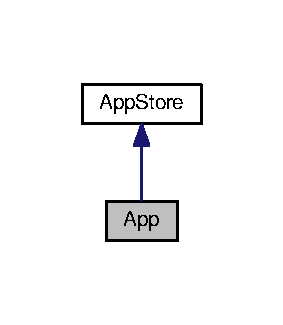
\includegraphics[width=136pt]{class_app__inherit__graph}
\end{center}
\end{figure}


Collaboration diagram for App\-:
\nopagebreak
\begin{figure}[H]
\begin{center}
\leavevmode
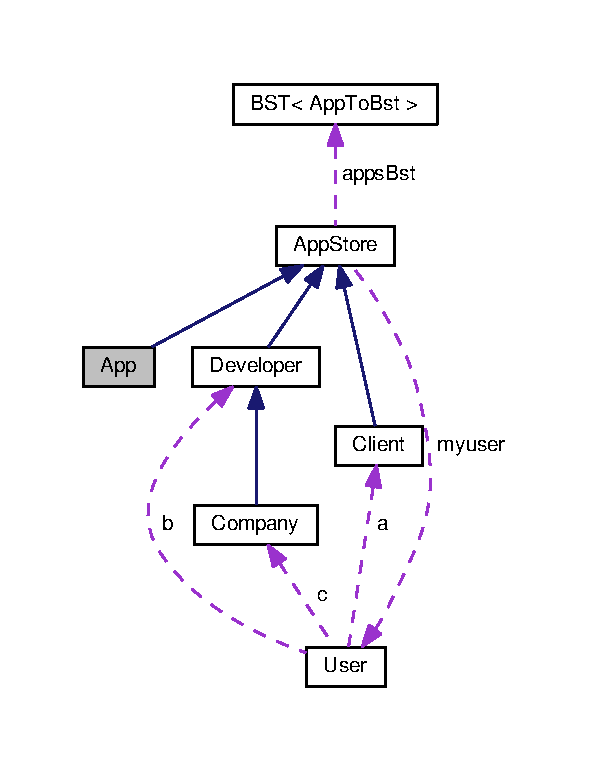
\includegraphics[width=283pt]{class_app__coll__graph}
\end{center}
\end{figure}
\subsection*{Public Member Functions}
\begin{DoxyCompactItemize}
\item 
\hyperlink{class_app_acb8cbf3e285b91d0170ffe87df5989c5}{App} ()
\begin{DoxyCompactList}\small\item\em Creates an object of \hyperlink{class_app}{App} class. \end{DoxyCompactList}\item 
\hyperlink{class_app_aa3731a04a7b0acb38a20babef71be4b2}{App} (string n, float co, string ca, string di, bool b, float classific=0)
\begin{DoxyCompactList}\small\item\em Creates an object of \hyperlink{class_app}{App} class. \end{DoxyCompactList}\item 
float \hyperlink{class_app_a9ca40e442fead18c4912c043bb3eec0c}{get\-Classification} () const 
\begin{DoxyCompactList}\small\item\em Gets classification. \end{DoxyCompactList}\item 
void \hyperlink{class_app_a175d65b6341257216b3b366d12623f40}{set\-Classification} (float a)
\begin{DoxyCompactList}\small\item\em Sets Classification. \end{DoxyCompactList}\item 
string \hyperlink{class_app_a32eb5fb345735dd5545e31e540b00969}{get\-Name} () const 
\begin{DoxyCompactList}\small\item\em gets the name of the app \end{DoxyCompactList}\item 
void \hyperlink{class_app_a960a18b2a0582166cff18b11e6572607}{set\-Name} (string n)
\begin{DoxyCompactList}\small\item\em Sets the name of the \hyperlink{class_app}{App}. \end{DoxyCompactList}\item 
float \hyperlink{class_app_a59d402c9a9f578f0c031bbee0c029d8a}{get\-Cost} () const 
\begin{DoxyCompactList}\small\item\em Gets the cost of the \hyperlink{class_app}{App}. \end{DoxyCompactList}\item 
void \hyperlink{class_app_a388b33b55bfb1c44ddaf8142f6164477}{set\-Cost} (float c)
\begin{DoxyCompactList}\small\item\em Sets the cost of the \hyperlink{class_app}{App}. \end{DoxyCompactList}\item 
string \hyperlink{class_app_aaca45decd05fd41da9317b5e9f5add7b}{get\-Category} () const 
\begin{DoxyCompactList}\small\item\em Gets the \hyperlink{class_app}{App} category. \end{DoxyCompactList}\item 
void \hyperlink{class_app_a361a6aa87af3a81d500a3d8f67b6940c}{set\-Category} (string cat)
\begin{DoxyCompactList}\small\item\em Sets the category. \end{DoxyCompactList}\item 
string \hyperlink{class_app_acbd6cc03ee6fe958227ea45344e078b0}{get\-Description} () const 
\begin{DoxyCompactList}\small\item\em Gets the description of the \hyperlink{class_app}{App}. \end{DoxyCompactList}\item 
void \hyperlink{class_app_a24d1eb228d32fef3d98e92a66970cfa2}{set\-Description} (string desc)
\begin{DoxyCompactList}\small\item\em Sets the Apps description. \end{DoxyCompactList}\item 
int \hyperlink{class_app_a3c036f3037aa6a9eac6d2bcdbffdb0c2}{get\-Id} () const 
\begin{DoxyCompactList}\small\item\em Gets the Apps Id. \end{DoxyCompactList}\item 
bool \hyperlink{class_app_a865521e2beed7cd13d036af5ac29a703}{get\-For\-Sale} () const 
\begin{DoxyCompactList}\small\item\em Gets the sale status of the \hyperlink{class_app}{App}. \end{DoxyCompactList}\item 
void \hyperlink{class_app_a63a422b19431fe206619be2090d6180a}{set\-For\-Sale} (bool b)
\begin{DoxyCompactList}\small\item\em Sets the sale status of the \hyperlink{class_app}{App}. \end{DoxyCompactList}\item 
void \hyperlink{class_app_ae33d2eaf0ec742aa21d0e7bd47f074e0}{set\-Id} (int nid)
\begin{DoxyCompactList}\small\item\em Sets the Apps Id. \end{DoxyCompactList}\item 
int \hyperlink{class_app_ae79cb31ae791c1a066d311e5886107e0}{operator()} (const \hyperlink{class_app}{App} \&ap) const 
\begin{DoxyCompactList}\small\item\em gets the \%10 of the Apps Id \end{DoxyCompactList}\item 
bool \hyperlink{class_app_ae9b1238991da3af350ae40401582cfce}{operator()} (const \hyperlink{class_app}{App} \&ap1, const \hyperlink{class_app}{App} \&ap2) const 
\begin{DoxyCompactList}\small\item\em compares two Apps Id \end{DoxyCompactList}\item 
bool \hyperlink{class_app_af7034136954c95011efc0640c85e85a6}{operator$<$} (const \hyperlink{class_app}{App} a) const 
\begin{DoxyCompactList}\small\item\em Operator $<$ overload. \end{DoxyCompactList}\item 
bool \hyperlink{class_app_a90e591665075584afc0018403c7eabe8}{operator==} (const \hyperlink{class_app}{App} a) const 
\begin{DoxyCompactList}\small\item\em Operator == overload. \end{DoxyCompactList}\end{DoxyCompactItemize}
\subsection*{Additional Inherited Members}


\subsection{Detailed Description}


Definition at line 489 of file app\-Store.\-h.



\subsection{Constructor \& Destructor Documentation}
\hypertarget{class_app_acb8cbf3e285b91d0170ffe87df5989c5}{\index{App@{App}!App@{App}}
\index{App@{App}!App@{App}}
\subsubsection[{App}]{\setlength{\rightskip}{0pt plus 5cm}App\-::\-App (
\begin{DoxyParamCaption}
{}
\end{DoxyParamCaption}
)}}\label{class_app_acb8cbf3e285b91d0170ffe87df5989c5}


Creates an object of \hyperlink{class_app}{App} class. 



Definition at line 136 of file app\-Store.\-cpp.

\hypertarget{class_app_aa3731a04a7b0acb38a20babef71be4b2}{\index{App@{App}!App@{App}}
\index{App@{App}!App@{App}}
\subsubsection[{App}]{\setlength{\rightskip}{0pt plus 5cm}App\-::\-App (
\begin{DoxyParamCaption}
\item[{string}]{n, }
\item[{float}]{co, }
\item[{string}]{ca, }
\item[{string}]{di, }
\item[{bool}]{b, }
\item[{float}]{classific = {\ttfamily 0}}
\end{DoxyParamCaption}
)}}\label{class_app_aa3731a04a7b0acb38a20babef71be4b2}


Creates an object of \hyperlink{class_app}{App} class. 


\begin{DoxyParams}{Parameters}
{\em n} & Name \\
\hline
{\em co} & cost \\
\hline
{\em ca} & category \\
\hline
{\em di} & discription \\
\hline
{\em b} & bool \\
\hline
{\em classif} & 0 \\
\hline
\end{DoxyParams}


Definition at line 145 of file app\-Store.\-cpp.



\subsection{Member Function Documentation}
\hypertarget{class_app_aaca45decd05fd41da9317b5e9f5add7b}{\index{App@{App}!get\-Category@{get\-Category}}
\index{get\-Category@{get\-Category}!App@{App}}
\subsubsection[{get\-Category}]{\setlength{\rightskip}{0pt plus 5cm}string App\-::get\-Category (
\begin{DoxyParamCaption}
{}
\end{DoxyParamCaption}
) const}}\label{class_app_aaca45decd05fd41da9317b5e9f5add7b}


Gets the \hyperlink{class_app}{App} category. 

\begin{DoxyReturn}{Returns}
Returns the Apps category 
\end{DoxyReturn}


Definition at line 172 of file app\-Store.\-cpp.

\hypertarget{class_app_a9ca40e442fead18c4912c043bb3eec0c}{\index{App@{App}!get\-Classification@{get\-Classification}}
\index{get\-Classification@{get\-Classification}!App@{App}}
\subsubsection[{get\-Classification}]{\setlength{\rightskip}{0pt plus 5cm}float App\-::get\-Classification (
\begin{DoxyParamCaption}
{}
\end{DoxyParamCaption}
) const\hspace{0.3cm}{\ttfamily [inline]}}}\label{class_app_a9ca40e442fead18c4912c043bb3eec0c}


Gets classification. 

\begin{DoxyReturn}{Returns}
classification 
\end{DoxyReturn}


Definition at line 518 of file app\-Store.\-h.

\hypertarget{class_app_a59d402c9a9f578f0c031bbee0c029d8a}{\index{App@{App}!get\-Cost@{get\-Cost}}
\index{get\-Cost@{get\-Cost}!App@{App}}
\subsubsection[{get\-Cost}]{\setlength{\rightskip}{0pt plus 5cm}float App\-::get\-Cost (
\begin{DoxyParamCaption}
{}
\end{DoxyParamCaption}
) const}}\label{class_app_a59d402c9a9f578f0c031bbee0c029d8a}


Gets the cost of the \hyperlink{class_app}{App}. 



Definition at line 164 of file app\-Store.\-cpp.

\hypertarget{class_app_acbd6cc03ee6fe958227ea45344e078b0}{\index{App@{App}!get\-Description@{get\-Description}}
\index{get\-Description@{get\-Description}!App@{App}}
\subsubsection[{get\-Description}]{\setlength{\rightskip}{0pt plus 5cm}string App\-::get\-Description (
\begin{DoxyParamCaption}
{}
\end{DoxyParamCaption}
) const}}\label{class_app_acbd6cc03ee6fe958227ea45344e078b0}


Gets the description of the \hyperlink{class_app}{App}. 

\begin{DoxyReturn}{Returns}
Returns the Apps description 
\end{DoxyReturn}


Definition at line 180 of file app\-Store.\-cpp.

\hypertarget{class_app_a865521e2beed7cd13d036af5ac29a703}{\index{App@{App}!get\-For\-Sale@{get\-For\-Sale}}
\index{get\-For\-Sale@{get\-For\-Sale}!App@{App}}
\subsubsection[{get\-For\-Sale}]{\setlength{\rightskip}{0pt plus 5cm}bool App\-::get\-For\-Sale (
\begin{DoxyParamCaption}
{}
\end{DoxyParamCaption}
) const}}\label{class_app_a865521e2beed7cd13d036af5ac29a703}


Gets the sale status of the \hyperlink{class_app}{App}. 

\begin{DoxyReturn}{Returns}
Returns true if for sale 
\end{DoxyReturn}


Definition at line 192 of file app\-Store.\-cpp.

\hypertarget{class_app_a3c036f3037aa6a9eac6d2bcdbffdb0c2}{\index{App@{App}!get\-Id@{get\-Id}}
\index{get\-Id@{get\-Id}!App@{App}}
\subsubsection[{get\-Id}]{\setlength{\rightskip}{0pt plus 5cm}int App\-::get\-Id (
\begin{DoxyParamCaption}
{}
\end{DoxyParamCaption}
) const}}\label{class_app_a3c036f3037aa6a9eac6d2bcdbffdb0c2}


Gets the Apps Id. 

\begin{DoxyReturn}{Returns}
Returns the Apps Id 
\end{DoxyReturn}


Definition at line 188 of file app\-Store.\-cpp.

\hypertarget{class_app_a32eb5fb345735dd5545e31e540b00969}{\index{App@{App}!get\-Name@{get\-Name}}
\index{get\-Name@{get\-Name}!App@{App}}
\subsubsection[{get\-Name}]{\setlength{\rightskip}{0pt plus 5cm}string App\-::get\-Name (
\begin{DoxyParamCaption}
{}
\end{DoxyParamCaption}
) const}}\label{class_app_a32eb5fb345735dd5545e31e540b00969}


gets the name of the app 

\begin{DoxyReturn}{Returns}
Returns the name of the \hyperlink{class_app}{App} 
\end{DoxyReturn}


Definition at line 156 of file app\-Store.\-cpp.

\hypertarget{class_app_ae79cb31ae791c1a066d311e5886107e0}{\index{App@{App}!operator()@{operator()}}
\index{operator()@{operator()}!App@{App}}
\subsubsection[{operator()}]{\setlength{\rightskip}{0pt plus 5cm}int App\-::operator() (
\begin{DoxyParamCaption}
\item[{const {\bf App} \&}]{ap}
\end{DoxyParamCaption}
) const\hspace{0.3cm}{\ttfamily [inline]}}}\label{class_app_ae79cb31ae791c1a066d311e5886107e0}


gets the \%10 of the Apps Id 

\begin{DoxyReturn}{Returns}
Returns the \%10 of the Apps Id 
\end{DoxyReturn}


Definition at line 602 of file app\-Store.\-h.

\hypertarget{class_app_ae9b1238991da3af350ae40401582cfce}{\index{App@{App}!operator()@{operator()}}
\index{operator()@{operator()}!App@{App}}
\subsubsection[{operator()}]{\setlength{\rightskip}{0pt plus 5cm}bool App\-::operator() (
\begin{DoxyParamCaption}
\item[{const {\bf App} \&}]{ap1, }
\item[{const {\bf App} \&}]{ap2}
\end{DoxyParamCaption}
) const\hspace{0.3cm}{\ttfamily [inline]}}}\label{class_app_ae9b1238991da3af350ae40401582cfce}


compares two Apps Id 

\begin{DoxyReturn}{Returns}
Returns true if Id1 == Id2 
\end{DoxyReturn}


Definition at line 611 of file app\-Store.\-h.

\hypertarget{class_app_af7034136954c95011efc0640c85e85a6}{\index{App@{App}!operator$<$@{operator$<$}}
\index{operator$<$@{operator$<$}!App@{App}}
\subsubsection[{operator$<$}]{\setlength{\rightskip}{0pt plus 5cm}bool App\-::operator$<$ (
\begin{DoxyParamCaption}
\item[{const {\bf App}}]{a}
\end{DoxyParamCaption}
) const}}\label{class_app_af7034136954c95011efc0640c85e85a6}


Operator $<$ overload. 


\begin{DoxyParams}{Parameters}
{\em a} & \hyperlink{class_app}{App}\\
\hline
\end{DoxyParams}
\begin{DoxyReturn}{Returns}
Returns true if first $<$ second 
\end{DoxyReturn}


Definition at line 1689 of file app\-Store.\-cpp.

\hypertarget{class_app_a90e591665075584afc0018403c7eabe8}{\index{App@{App}!operator==@{operator==}}
\index{operator==@{operator==}!App@{App}}
\subsubsection[{operator==}]{\setlength{\rightskip}{0pt plus 5cm}bool App\-::operator== (
\begin{DoxyParamCaption}
\item[{const {\bf App}}]{a}
\end{DoxyParamCaption}
) const}}\label{class_app_a90e591665075584afc0018403c7eabe8}


Operator == overload. 


\begin{DoxyParams}{Parameters}
{\em a} & \hyperlink{class_app}{App}\\
\hline
\end{DoxyParams}
\begin{DoxyReturn}{Returns}
Returns true if first == second 
\end{DoxyReturn}


Definition at line 1685 of file app\-Store.\-cpp.

\hypertarget{class_app_a361a6aa87af3a81d500a3d8f67b6940c}{\index{App@{App}!set\-Category@{set\-Category}}
\index{set\-Category@{set\-Category}!App@{App}}
\subsubsection[{set\-Category}]{\setlength{\rightskip}{0pt plus 5cm}void App\-::set\-Category (
\begin{DoxyParamCaption}
\item[{string}]{cat}
\end{DoxyParamCaption}
)}}\label{class_app_a361a6aa87af3a81d500a3d8f67b6940c}


Sets the category. 


\begin{DoxyParams}{Parameters}
{\em cat} & category to set \\
\hline
\end{DoxyParams}


Definition at line 176 of file app\-Store.\-cpp.

\hypertarget{class_app_a175d65b6341257216b3b366d12623f40}{\index{App@{App}!set\-Classification@{set\-Classification}}
\index{set\-Classification@{set\-Classification}!App@{App}}
\subsubsection[{set\-Classification}]{\setlength{\rightskip}{0pt plus 5cm}void App\-::set\-Classification (
\begin{DoxyParamCaption}
\item[{float}]{a}
\end{DoxyParamCaption}
)\hspace{0.3cm}{\ttfamily [inline]}}}\label{class_app_a175d65b6341257216b3b366d12623f40}


Sets Classification. 


\begin{DoxyParams}{Parameters}
{\em a} & classification \\
\hline
\end{DoxyParams}


Definition at line 524 of file app\-Store.\-h.

\hypertarget{class_app_a388b33b55bfb1c44ddaf8142f6164477}{\index{App@{App}!set\-Cost@{set\-Cost}}
\index{set\-Cost@{set\-Cost}!App@{App}}
\subsubsection[{set\-Cost}]{\setlength{\rightskip}{0pt plus 5cm}void App\-::set\-Cost (
\begin{DoxyParamCaption}
\item[{float}]{c}
\end{DoxyParamCaption}
)}}\label{class_app_a388b33b55bfb1c44ddaf8142f6164477}


Sets the cost of the \hyperlink{class_app}{App}. 


\begin{DoxyParams}{Parameters}
{\em c} & cost of the \hyperlink{class_app}{App} to set \\
\hline
\end{DoxyParams}


Definition at line 168 of file app\-Store.\-cpp.

\hypertarget{class_app_a24d1eb228d32fef3d98e92a66970cfa2}{\index{App@{App}!set\-Description@{set\-Description}}
\index{set\-Description@{set\-Description}!App@{App}}
\subsubsection[{set\-Description}]{\setlength{\rightskip}{0pt plus 5cm}void App\-::set\-Description (
\begin{DoxyParamCaption}
\item[{string}]{desc}
\end{DoxyParamCaption}
)}}\label{class_app_a24d1eb228d32fef3d98e92a66970cfa2}


Sets the Apps description. 

\begin{DoxyReturn}{Returns}
Returns the Apps description 
\end{DoxyReturn}


Definition at line 184 of file app\-Store.\-cpp.

\hypertarget{class_app_a63a422b19431fe206619be2090d6180a}{\index{App@{App}!set\-For\-Sale@{set\-For\-Sale}}
\index{set\-For\-Sale@{set\-For\-Sale}!App@{App}}
\subsubsection[{set\-For\-Sale}]{\setlength{\rightskip}{0pt plus 5cm}void App\-::set\-For\-Sale (
\begin{DoxyParamCaption}
\item[{bool}]{b}
\end{DoxyParamCaption}
)}}\label{class_app_a63a422b19431fe206619be2090d6180a}


Sets the sale status of the \hyperlink{class_app}{App}. 


\begin{DoxyParams}{Parameters}
{\em b} & the status to set \\
\hline
\end{DoxyParams}


Definition at line 196 of file app\-Store.\-cpp.

\hypertarget{class_app_ae33d2eaf0ec742aa21d0e7bd47f074e0}{\index{App@{App}!set\-Id@{set\-Id}}
\index{set\-Id@{set\-Id}!App@{App}}
\subsubsection[{set\-Id}]{\setlength{\rightskip}{0pt plus 5cm}void App\-::set\-Id (
\begin{DoxyParamCaption}
\item[{int}]{nid}
\end{DoxyParamCaption}
)\hspace{0.3cm}{\ttfamily [inline]}}}\label{class_app_ae33d2eaf0ec742aa21d0e7bd47f074e0}


Sets the Apps Id. 


\begin{DoxyParams}{Parameters}
{\em nid} & Id to set \\
\hline
\end{DoxyParams}


Definition at line 594 of file app\-Store.\-h.

\hypertarget{class_app_a960a18b2a0582166cff18b11e6572607}{\index{App@{App}!set\-Name@{set\-Name}}
\index{set\-Name@{set\-Name}!App@{App}}
\subsubsection[{set\-Name}]{\setlength{\rightskip}{0pt plus 5cm}void App\-::set\-Name (
\begin{DoxyParamCaption}
\item[{string}]{n}
\end{DoxyParamCaption}
)}}\label{class_app_a960a18b2a0582166cff18b11e6572607}


Sets the name of the \hyperlink{class_app}{App}. 


\begin{DoxyParams}{Parameters}
{\em n} & name to set \\
\hline
\end{DoxyParams}


Definition at line 160 of file app\-Store.\-cpp.



The documentation for this class was generated from the following files\-:\begin{DoxyCompactItemize}
\item 
src/\hyperlink{app_store_8h}{app\-Store.\-h}\item 
src/\hyperlink{app_store_8cpp}{app\-Store.\-cpp}\end{DoxyCompactItemize}

\hypertarget{class_app_for_submission}{\section{App\-For\-Submission Class Reference}
\label{class_app_for_submission}\index{App\-For\-Submission@{App\-For\-Submission}}
}


{\ttfamily \#include $<$app\-Store.\-h$>$}

\subsection*{Public Member Functions}
\begin{DoxyCompactItemize}
\item 
\hyperlink{class_app_for_submission_a5fae87af61b79da9e893ccf656af8e6b}{App\-For\-Submission} ()
\begin{DoxyCompactList}\small\item\em Creates an object of \hyperlink{class_app_for_submission}{App\-For\-Submission} class. \end{DoxyCompactList}\item 
\hyperlink{class_app_for_submission_a473949659cefa64245784f9a9d15ee9a}{App\-For\-Submission} (\hyperlink{class_app}{App} a, \hyperlink{struct_date}{Date} sd, string u\-Name)
\begin{DoxyCompactList}\small\item\em Creates an object of \hyperlink{class_app_for_submission}{App\-For\-Submission} class. \end{DoxyCompactList}\item 
bool \hyperlink{class_app_for_submission_aeec3c2f36afaad540b518f720083b946}{operator$<$} (\hyperlink{class_app_for_submission}{App\-For\-Submission} const \&b) const 
\begin{DoxyCompactList}\small\item\em Operator $<$ overload. \end{DoxyCompactList}\item 
\hyperlink{class_app}{App} \hyperlink{class_app_for_submission_a28d8e59fa04846c4418b2320f25c5bb7}{get\-App} () const 
\begin{DoxyCompactList}\small\item\em Gets the \hyperlink{class_app}{App}. \end{DoxyCompactList}\item 
\hyperlink{struct_date}{Date} \hyperlink{class_app_for_submission_ac58170a02a427f2e26273bbec0f6b5c3}{get\-Sub\-Date} () const 
\begin{DoxyCompactList}\small\item\em Gets sub date. \end{DoxyCompactList}\item 
string \hyperlink{class_app_for_submission_a0779d0ae71facc527bac4ed5552023b7}{get\-Username} () const 
\begin{DoxyCompactList}\small\item\em Get the users name. \end{DoxyCompactList}\item 
void \hyperlink{class_app_for_submission_a58d658f2182d568c330d0535eb8aab42}{set\-App} (string appname, float cost, string cat, string desc)
\begin{DoxyCompactList}\small\item\em Sets the \hyperlink{class_app}{App}. \end{DoxyCompactList}\end{DoxyCompactItemize}


\subsection{Detailed Description}


Definition at line 635 of file app\-Store.\-h.



\subsection{Constructor \& Destructor Documentation}
\hypertarget{class_app_for_submission_a5fae87af61b79da9e893ccf656af8e6b}{\index{App\-For\-Submission@{App\-For\-Submission}!App\-For\-Submission@{App\-For\-Submission}}
\index{App\-For\-Submission@{App\-For\-Submission}!AppForSubmission@{App\-For\-Submission}}
\subsubsection[{App\-For\-Submission}]{\setlength{\rightskip}{0pt plus 5cm}App\-For\-Submission\-::\-App\-For\-Submission (
\begin{DoxyParamCaption}
{}
\end{DoxyParamCaption}
)\hspace{0.3cm}{\ttfamily [inline]}}}\label{class_app_for_submission_a5fae87af61b79da9e893ccf656af8e6b}


Creates an object of \hyperlink{class_app_for_submission}{App\-For\-Submission} class. 



Definition at line 643 of file app\-Store.\-h.

\hypertarget{class_app_for_submission_a473949659cefa64245784f9a9d15ee9a}{\index{App\-For\-Submission@{App\-For\-Submission}!App\-For\-Submission@{App\-For\-Submission}}
\index{App\-For\-Submission@{App\-For\-Submission}!AppForSubmission@{App\-For\-Submission}}
\subsubsection[{App\-For\-Submission}]{\setlength{\rightskip}{0pt plus 5cm}App\-For\-Submission\-::\-App\-For\-Submission (
\begin{DoxyParamCaption}
\item[{{\bf App}}]{a, }
\item[{{\bf Date}}]{sd, }
\item[{string}]{u\-Name}
\end{DoxyParamCaption}
)}}\label{class_app_for_submission_a473949659cefa64245784f9a9d15ee9a}


Creates an object of \hyperlink{class_app_for_submission}{App\-For\-Submission} class. 


\begin{DoxyParams}{Parameters}
{\em a} & \hyperlink{class_app}{App} \\
\hline
{\em sd} & date of insertion \\
\hline
{\em u\-Name} & user name \\
\hline
\end{DoxyParams}


Definition at line 202 of file app\-Store.\-cpp.



\subsection{Member Function Documentation}
\hypertarget{class_app_for_submission_a28d8e59fa04846c4418b2320f25c5bb7}{\index{App\-For\-Submission@{App\-For\-Submission}!get\-App@{get\-App}}
\index{get\-App@{get\-App}!AppForSubmission@{App\-For\-Submission}}
\subsubsection[{get\-App}]{\setlength{\rightskip}{0pt plus 5cm}{\bf App} App\-For\-Submission\-::get\-App (
\begin{DoxyParamCaption}
{}
\end{DoxyParamCaption}
) const\hspace{0.3cm}{\ttfamily [inline]}}}\label{class_app_for_submission_a28d8e59fa04846c4418b2320f25c5bb7}


Gets the \hyperlink{class_app}{App}. 

\begin{DoxyReturn}{Returns}
Returns an \hyperlink{class_app}{App} 
\end{DoxyReturn}


Definition at line 669 of file app\-Store.\-h.

\hypertarget{class_app_for_submission_ac58170a02a427f2e26273bbec0f6b5c3}{\index{App\-For\-Submission@{App\-For\-Submission}!get\-Sub\-Date@{get\-Sub\-Date}}
\index{get\-Sub\-Date@{get\-Sub\-Date}!AppForSubmission@{App\-For\-Submission}}
\subsubsection[{get\-Sub\-Date}]{\setlength{\rightskip}{0pt plus 5cm}{\bf Date} App\-For\-Submission\-::get\-Sub\-Date (
\begin{DoxyParamCaption}
{}
\end{DoxyParamCaption}
) const\hspace{0.3cm}{\ttfamily [inline]}}}\label{class_app_for_submission_ac58170a02a427f2e26273bbec0f6b5c3}


Gets sub date. 

\begin{DoxyReturn}{Returns}
Returns the submission date 
\end{DoxyReturn}


Definition at line 675 of file app\-Store.\-h.

\hypertarget{class_app_for_submission_a0779d0ae71facc527bac4ed5552023b7}{\index{App\-For\-Submission@{App\-For\-Submission}!get\-Username@{get\-Username}}
\index{get\-Username@{get\-Username}!AppForSubmission@{App\-For\-Submission}}
\subsubsection[{get\-Username}]{\setlength{\rightskip}{0pt plus 5cm}string App\-For\-Submission\-::get\-Username (
\begin{DoxyParamCaption}
{}
\end{DoxyParamCaption}
) const\hspace{0.3cm}{\ttfamily [inline]}}}\label{class_app_for_submission_a0779d0ae71facc527bac4ed5552023b7}


Get the users name. 

\begin{DoxyReturn}{Returns}
Returns the users name 
\end{DoxyReturn}


Definition at line 681 of file app\-Store.\-h.

\hypertarget{class_app_for_submission_aeec3c2f36afaad540b518f720083b946}{\index{App\-For\-Submission@{App\-For\-Submission}!operator$<$@{operator$<$}}
\index{operator$<$@{operator$<$}!AppForSubmission@{App\-For\-Submission}}
\subsubsection[{operator$<$}]{\setlength{\rightskip}{0pt plus 5cm}bool App\-For\-Submission\-::operator$<$ (
\begin{DoxyParamCaption}
\item[{{\bf App\-For\-Submission} const \&}]{b}
\end{DoxyParamCaption}
) const}}\label{class_app_for_submission_aeec3c2f36afaad540b518f720083b946}


Operator $<$ overload. 


\begin{DoxyParams}{Parameters}
{\em b} & \hyperlink{class_app_for_submission}{App\-For\-Submission}\\
\hline
\end{DoxyParams}
\begin{DoxyReturn}{Returns}
Returnstrue if first $<$ sencond 
\end{DoxyReturn}


Definition at line 204 of file app\-Store.\-cpp.

\hypertarget{class_app_for_submission_a58d658f2182d568c330d0535eb8aab42}{\index{App\-For\-Submission@{App\-For\-Submission}!set\-App@{set\-App}}
\index{set\-App@{set\-App}!AppForSubmission@{App\-For\-Submission}}
\subsubsection[{set\-App}]{\setlength{\rightskip}{0pt plus 5cm}void App\-For\-Submission\-::set\-App (
\begin{DoxyParamCaption}
\item[{string}]{appname, }
\item[{float}]{cost, }
\item[{string}]{cat, }
\item[{string}]{desc}
\end{DoxyParamCaption}
)\hspace{0.3cm}{\ttfamily [inline]}}}\label{class_app_for_submission_a58d658f2182d568c330d0535eb8aab42}


Sets the \hyperlink{class_app}{App}. 


\begin{DoxyParams}{Parameters}
{\em appname} & Apps name \\
\hline
{\em cost} & Apps cost \\
\hline
{\em cat} & Apps category \\
\hline
{\em desc} & Apps description \\
\hline
\end{DoxyParams}


Definition at line 690 of file app\-Store.\-h.



The documentation for this class was generated from the following files\-:\begin{DoxyCompactItemize}
\item 
src/\hyperlink{app_store_8h}{app\-Store.\-h}\item 
src/\hyperlink{app_store_8cpp}{app\-Store.\-cpp}\end{DoxyCompactItemize}

\hypertarget{class_app_not_found}{\section{App\-Not\-Found Class Reference}
\label{class_app_not_found}\index{App\-Not\-Found@{App\-Not\-Found}}
}


{\ttfamily \#include $<$app\-Store.\-h$>$}

\subsection*{Public Member Functions}
\begin{DoxyCompactItemize}
\item 
\hyperlink{class_app_not_found_ad3acd5d6a5e9b510d085557b4d9d4284}{App\-Not\-Found} (string dev)
\begin{DoxyCompactList}\small\item\em Creates an objecto (exception) of class \hyperlink{class_app_not_found}{App\-Not\-Found}. \end{DoxyCompactList}\end{DoxyCompactItemize}
\subsection*{Public Attributes}
\begin{DoxyCompactItemize}
\item 
string \hyperlink{class_app_not_found_aa6c5acb8dbaf037e57aed9f0e0870af5}{name}
\end{DoxyCompactItemize}


\subsection{Detailed Description}


Definition at line 1117 of file app\-Store.\-h.



\subsection{Constructor \& Destructor Documentation}
\hypertarget{class_app_not_found_ad3acd5d6a5e9b510d085557b4d9d4284}{\index{App\-Not\-Found@{App\-Not\-Found}!App\-Not\-Found@{App\-Not\-Found}}
\index{App\-Not\-Found@{App\-Not\-Found}!AppNotFound@{App\-Not\-Found}}
\subsubsection[{App\-Not\-Found}]{\setlength{\rightskip}{0pt plus 5cm}App\-Not\-Found\-::\-App\-Not\-Found (
\begin{DoxyParamCaption}
\item[{string}]{dev}
\end{DoxyParamCaption}
)\hspace{0.3cm}{\ttfamily [inline]}}}\label{class_app_not_found_ad3acd5d6a5e9b510d085557b4d9d4284}


Creates an objecto (exception) of class \hyperlink{class_app_not_found}{App\-Not\-Found}. 


\begin{DoxyParams}{Parameters}
{\em n} & developer \\
\hline
\end{DoxyParams}


Definition at line 1125 of file app\-Store.\-h.



\subsection{Member Data Documentation}
\hypertarget{class_app_not_found_aa6c5acb8dbaf037e57aed9f0e0870af5}{\index{App\-Not\-Found@{App\-Not\-Found}!name@{name}}
\index{name@{name}!AppNotFound@{App\-Not\-Found}}
\subsubsection[{name}]{\setlength{\rightskip}{0pt plus 5cm}string App\-Not\-Found\-::name}}\label{class_app_not_found_aa6c5acb8dbaf037e57aed9f0e0870af5}


Definition at line 1119 of file app\-Store.\-h.



The documentation for this class was generated from the following file\-:\begin{DoxyCompactItemize}
\item 
src/\hyperlink{app_store_8h}{app\-Store.\-h}\end{DoxyCompactItemize}

\hypertarget{class_app_store}{\section{App\-Store Class Reference}
\label{class_app_store}\index{App\-Store@{App\-Store}}
}


{\ttfamily \#include $<$app\-Store.\-h$>$}



Inheritance diagram for App\-Store\-:
\nopagebreak
\begin{figure}[H]
\begin{center}
\leavevmode
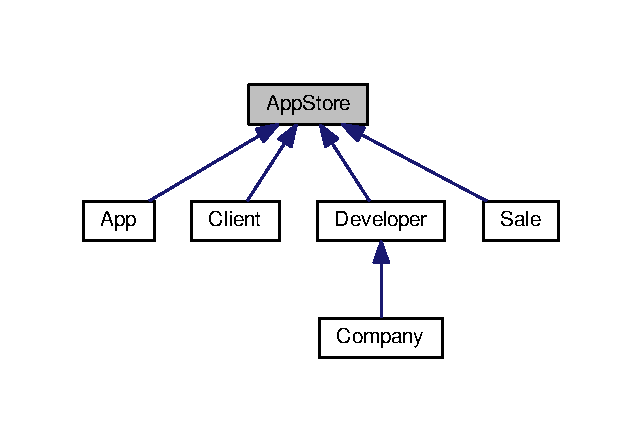
\includegraphics[width=308pt]{class_app_store__inherit__graph}
\end{center}
\end{figure}


Collaboration diagram for App\-Store\-:
\nopagebreak
\begin{figure}[H]
\begin{center}
\leavevmode
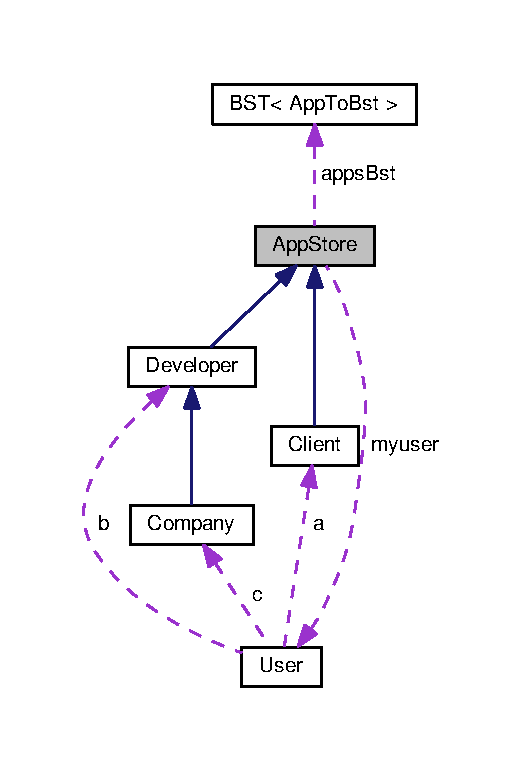
\includegraphics[width=251pt]{class_app_store__coll__graph}
\end{center}
\end{figure}
\subsection*{Public Member Functions}
\begin{DoxyCompactItemize}
\item 
\hyperlink{class_app_store_ac94669ac551c6862db7f3636fc86ae8e}{App\-Store} ()
\begin{DoxyCompactList}\small\item\em creates an \hyperlink{class_app}{App} \end{DoxyCompactList}\item 
bool \hyperlink{class_app_store_acf9313158ff9ebf261d92b51248d5929}{create\-App} ()
\begin{DoxyCompactList}\small\item\em Creates an \hyperlink{class_app}{App} asking for its atributes. \end{DoxyCompactList}\item 
void \hyperlink{class_app_store_a7e8ba8e462d02b31196055aff69b3eba}{read\-App} ()
\begin{DoxyCompactList}\small\item\em Reads the info of an \hyperlink{class_app}{App}. \end{DoxyCompactList}\item 
bool \hyperlink{class_app_store_ae2993b78d05d2418d76d22f9ced7330f}{update\-App} ()
\item 
bool \hyperlink{class_app_store_ae36a7cf8a9304a1119164bc634c7dd07}{delete\-App} ()
\item 
void \hyperlink{class_app_store_a45df3300374af488440ee24302da6186}{show\-All\-Apps} () const 
\begin{DoxyCompactList}\small\item\em Shows all Apps. \end{DoxyCompactList}\item 
void \hyperlink{class_app_store_a2de414f5e07ece6a35b71c2118355da5}{validate\-App} ()
\item 
void \hyperlink{class_app_store_ad699f59e9ebb9d187463453c21c4fa90}{read\-App\-Waiting\-Approval} ()
\begin{DoxyCompactList}\small\item\em Display info on 1 \hyperlink{class_app}{App} waiting to be aproved. \end{DoxyCompactList}\item 
void \hyperlink{class_app_store_af35d08900aea40cdf7f50949cfc0edd0}{delete\-App\-Waiting\-Approval} ()
\begin{DoxyCompactList}\small\item\em Deletes an \hyperlink{class_app}{App} that is waiting for Aproval. \end{DoxyCompactList}\item 
void \hyperlink{class_app_store_aa3dcdac081b1e94a59ea9c03a93f9a72}{show\-All\-Apps\-Waiting\-Approval} () const 
\begin{DoxyCompactList}\small\item\em Displays the list of all Apps waiting for approval. \end{DoxyCompactList}\item 
void \hyperlink{class_app_store_a8a1bd45c8da47c28c573fee0ceb3720a}{update\-App\-Waiting\-Approval} ()
\begin{DoxyCompactList}\small\item\em Updates one of the Apps waiting for approval. \end{DoxyCompactList}\item 
bool \hyperlink{class_app_store_ab9ae4acba7e7bf74e92e9dfb083acd4b}{create\-Client} ()
\begin{DoxyCompactList}\small\item\em Creates a \hyperlink{class_client}{Client} -\/ C\-R\-U\-D. \end{DoxyCompactList}\item 
void \hyperlink{class_app_store_aecb3bdf89a8b5d772c6677816731763d}{read\-Client} ()
\begin{DoxyCompactList}\small\item\em Reads intel on a \hyperlink{class_client}{Client} -\/ C\-R\-U\-D. \end{DoxyCompactList}\item 
bool \hyperlink{class_app_store_a2c03b4be04c9b3e8ff063b3372941b5c}{update\-Client} ()
\begin{DoxyCompactList}\small\item\em Updates a \hyperlink{class_client}{Client} -\/ C\-R\-U\-D. \end{DoxyCompactList}\item 
bool \hyperlink{class_app_store_a45233b575b02d5337bf8837844e771b5}{delete\-Client} ()
\begin{DoxyCompactList}\small\item\em Deletes a \hyperlink{class_client}{Client} -\/ C\-R\-U\-D. \end{DoxyCompactList}\item 
void \hyperlink{class_app_store_ad8d1df5f575e231df889328b501d836d}{show\-All\-Clients} () const 
\begin{DoxyCompactList}\small\item\em Shows the list of all Clients -\/ C\-R\-U\-D. \end{DoxyCompactList}\item 
bool \hyperlink{class_app_store_ab378b7986b83da52f332ac5a2799a6e5}{create\-Developer} ()
\begin{DoxyCompactList}\small\item\em Creates a \hyperlink{class_developer}{Developer} -\/ C\-R\-U\-D. \end{DoxyCompactList}\item 
void \hyperlink{class_app_store_a99fac835be3628e1731240269bc89210}{read\-Developer} ()
\begin{DoxyCompactList}\small\item\em Reads intel on a \hyperlink{class_developer}{Developer} -\/ C\-R\-U\-D. \end{DoxyCompactList}\item 
bool \hyperlink{class_app_store_aadd55aac42b87dc5ff85b8aec545e40d}{update\-Developer} ()
\begin{DoxyCompactList}\small\item\em Updates a Development -\/ C\-R\-U\-D. \end{DoxyCompactList}\item 
bool \hyperlink{class_app_store_ab23c0791d05005afb59b35aa2b0524ff}{delete\-Developer} ()
\begin{DoxyCompactList}\small\item\em Deletes a \hyperlink{class_developer}{Developer} -\/ C\-R\-U\-D. \end{DoxyCompactList}\item 
void \hyperlink{class_app_store_ad033cdc08a36cd98bfbfa2017990ef97}{show\-All\-Developers} () const 
\begin{DoxyCompactList}\small\item\em Shows all Developers -\/ C\-R\-U\-D. \end{DoxyCompactList}\item 
bool \hyperlink{class_app_store_aedcb4195dc5918718d628417e6b97b95}{create\-Company} ()
\begin{DoxyCompactList}\small\item\em Creates a \hyperlink{class_company}{Company} -\/ C\-R\-U\-D. \end{DoxyCompactList}\item 
void \hyperlink{class_app_store_a04f506638e8e949ce3a325cb5a6663ae}{read\-Company} ()
\begin{DoxyCompactList}\small\item\em Reads intel of a \hyperlink{class_company}{Company} -\/ C\-R\-U\-D. \end{DoxyCompactList}\item 
bool \hyperlink{class_app_store_a121e2731fa450585a9bf32cf97ede37b}{update\-Company} ()
\begin{DoxyCompactList}\small\item\em Updates a \hyperlink{class_company}{Company} -\/ C\-R\-U\-D. \end{DoxyCompactList}\item 
bool \hyperlink{class_app_store_a570764c37cc75a230f9c1efced300bc7}{delete\-Company} ()
\begin{DoxyCompactList}\small\item\em Deletes a \hyperlink{class_company}{Company} -\/ C\-R\-U\-D. \end{DoxyCompactList}\item 
void \hyperlink{class_app_store_ade086a2b1b96e6febb1bbe27d09311fc}{show\-All\-Companies} () const 
\begin{DoxyCompactList}\small\item\em Shows the list of all Companies -\/ C\-R\-U\-D. \end{DoxyCompactList}\item 
void \hyperlink{class_app_store_a1eab2532969e746083c95bf9343a88e2}{show\-All\-Sales} () const 
\begin{DoxyCompactList}\small\item\em Shows the list of all Sales -\/ C\-R\-U\-D. \end{DoxyCompactList}\item 
int \hyperlink{class_app_store_a2d33aa41da255cd2ad4732b5a908a71f}{find\-Index\-Client} (string n)
\begin{DoxyCompactList}\small\item\em Finds the index of the client in the respective vector. \end{DoxyCompactList}\item 
int \hyperlink{class_app_store_af2866f0d914b6ca1f0eddcfb427b3115}{find\-Index\-Developer} (string n)
\begin{DoxyCompactList}\small\item\em Finds the index of the \hyperlink{class_developer}{Developer} in the respective vector. \end{DoxyCompactList}\item 
int \hyperlink{class_app_store_a566fa7131765af151e3246e99f83593b}{find\-Index\-Dev\-User} (string n)
\begin{DoxyCompactList}\small\item\em Finds the index of the user in the respective vector. \end{DoxyCompactList}\item 
int \hyperlink{class_app_store_a6079f5467d811db32ecb60fac8e8aeaa}{find\-Index\-Company} (string n)
\begin{DoxyCompactList}\small\item\em Finds the index of the company in the respective vector. \end{DoxyCompactList}\item 
int \hyperlink{class_app_store_a872607cf250dd86d8566f8ed60a0b074}{find\-Index\-Comp\-User} (string n)
\begin{DoxyCompactList}\small\item\em Finds the index of the user in the respective vector. \end{DoxyCompactList}\item 
int \hyperlink{class_app_store_a20ab97effcf3ec46466b2e1cd08ab22f}{find\-Index\-App} (string n)
\begin{DoxyCompactList}\small\item\em Finds the index of the app in the respective vector. \end{DoxyCompactList}\item 
void \hyperlink{class_app_store_ad2da0413449f62341ab662b877c2a0dd}{erase\-App\-Developer} (int id)
\begin{DoxyCompactList}\small\item\em Deletes an app of the developers vector. \end{DoxyCompactList}\item 
void \hyperlink{class_app_store_a4e231329bc5d40d61ebb356bb9157213}{set\-App\-Classifications} ()
\begin{DoxyCompactList}\small\item\em Calculates the average of classification of each app. \end{DoxyCompactList}\item 
void \hyperlink{class_app_store_a759b4aab67d3d70a2458cce8b7c67347}{hash\-Insert} (\hyperlink{class_app}{App} $\ast$a)
\begin{DoxyCompactList}\small\item\em Inserts a in the hash. \end{DoxyCompactList}\item 
void \hyperlink{class_app_store_aa9a916366ddeb52170198c8d5ed3c1f8}{hash\-Remove} (\hyperlink{class_app}{App} $\ast$a)
\begin{DoxyCompactList}\small\item\em Removes a in the hash. \end{DoxyCompactList}\item 
priority\-\_\-queue$<$ \hyperlink{class_app_for_submission}{App\-For\-Submission} $>$ \hyperlink{class_app_store_a9b8feaee60fbbbf83535eb64f1aabcb5}{get\-Validation} ()
\begin{DoxyCompactList}\small\item\em Gets the queue of apps waiting validation. \end{DoxyCompactList}\item 
void \hyperlink{class_app_store_a405cb336f26ae96307f0d4a4d950930c}{show\-Top} ()
\begin{DoxyCompactList}\small\item\em Shows the top 10 Apps. \end{DoxyCompactList}\item 
void \hyperlink{class_app_store_abe0bf19e7ef9e84ae724ce3df2eca117}{apps\-To\-Bst} ()
\begin{DoxyCompactList}\small\item\em Frees the $\ast$\-App \hyperlink{class_b_s_t}{B\-S\-T} and replaces all Apps. \end{DoxyCompactList}\item 
void \hyperlink{class_app_store_aa9e324faa5f15af0f2ac3227607716be}{set\-Validation} (const priority\-\_\-queue$<$ \hyperlink{class_app_for_submission}{App\-For\-Submission} $>$ \&\hyperlink{class_app_store_a5aac74886d1170f360838aaa8428652b}{validation})
\begin{DoxyCompactList}\small\item\em Sets the validation status. \end{DoxyCompactList}\item 
void \hyperlink{class_app_store_aadcc50b226aa1a04b2fcc3f6ad07b3fc}{show\-Hash\-Apps} ()
\begin{DoxyCompactList}\small\item\em List apps from Hash Table. \end{DoxyCompactList}\item 
string \hyperlink{class_app_store_ad1d0983b2b3fba66a2876bf7df7b9cd5}{get\-Dev\-From\-App} (string name)
\begin{DoxyCompactList}\small\item\em Returns a Dev name giving dev app. \end{DoxyCompactList}\item 
void \hyperlink{class_app_store_a2e5f4c42b55c2dcb4e7e42f3cd45900c}{del\-Hash\-Apps} ()
\begin{DoxyCompactList}\small\item\em Deletes apps from hash tables. \end{DoxyCompactList}\item 
void \hyperlink{class_app_store_aec000285f1094e63b86a3d6753016d41}{update\-Hash\-Apps} ()
\begin{DoxyCompactList}\small\item\em Update Apps from Hash tables. \end{DoxyCompactList}\item 
bool \hyperlink{class_app_store_a8a1192683d74e8f4c9611adc6e0ca664}{exist} (string name)
\begin{DoxyCompactList}\small\item\em Checks if an \hyperlink{class_app}{App} exist. \end{DoxyCompactList}\item 
bool \hyperlink{class_app_store_a3f9e2b8cd4f0654cdb176250ee827b93}{dev\-Exist} (string name)
\begin{DoxyCompactList}\small\item\em Checks if a Dev exist. \end{DoxyCompactList}\item 
int \hyperlink{class_app_store_abbe21a1e0ad0bbeee3bdd0a280c1b72e}{create\-Hash\-Apps} ()
\begin{DoxyCompactList}\small\item\em Create apps to insert on the hash table and other data structure. \end{DoxyCompactList}\item 
void \hyperlink{class_app_store_a273c4ffa66b4b11ca90aaa392b08efb6}{Bst\-Reorganize} ()
\begin{DoxyCompactList}\small\item\em All arguments are inserted with correct order on \hyperlink{class_b_s_t}{B\-S\-T}. \end{DoxyCompactList}\item 
void \hyperlink{class_app_store_ad426df493048edf5d564a7a34cf38247}{Bst\-Remove} (int id)
\begin{DoxyCompactList}\small\item\em Remove an \hyperlink{class_app}{App} from \hyperlink{class_b_s_t}{B\-S\-T}. \end{DoxyCompactList}\item 
void \hyperlink{class_app_store_a4188dc3c042576ef220d7d26c0f55a35}{show\-Top10} ()
\begin{DoxyCompactList}\small\item\em Shows top 10 Apps from \hyperlink{class_b_s_t}{B\-S\-T}. \end{DoxyCompactList}\item 
\hyperlink{class_app}{App} \hyperlink{class_app_store_a39196e235f6f3c22808489d5ef1d516d}{get\-App} (int id)
\begin{DoxyCompactList}\small\item\em returns an \hyperlink{class_app}{App} from a giving I\-D \end{DoxyCompactList}\item 
void \hyperlink{class_app_store_aae1dc16347736d0021eade0569413ebe}{add\-To\-Bst} ()
\begin{DoxyCompactList}\small\item\em Add an \hyperlink{class_app}{App} to the \hyperlink{class_b_s_t}{B\-S\-T}. \end{DoxyCompactList}\item 
void \hyperlink{class_app_store_a0fdb4b829a446323909e0bfb61ec777b}{read\-Bst} ()
\begin{DoxyCompactList}\small\item\em Read from \hyperlink{class_b_s_t}{B\-S\-T}. \end{DoxyCompactList}\item 
void \hyperlink{class_app_store_a4218351acb8e17bb360f12e6415a557b}{remove\-From\-Bst} ()
\begin{DoxyCompactList}\small\item\em Remove an \hyperlink{class_app}{App} from \hyperlink{class_b_s_t}{B\-S\-T}. \end{DoxyCompactList}\end{DoxyCompactItemize}
\subsection*{Public Attributes}
\begin{DoxyCompactItemize}
\item 
vector$<$ \hyperlink{class_app}{App} $>$ \hyperlink{class_app_store_a4c7200eb18f1154bbe578840b89ad023}{All\-Time\-Apps}
\item 
vector$<$ \hyperlink{class_client}{Client} $>$ \hyperlink{class_app_store_adf4a143f08087c4b33b6e8de35c4c281}{clients}
\item 
vector$<$ \hyperlink{class_developer}{Developer} $>$ \hyperlink{class_app_store_addb4d854b56405d689398083b231bd19}{developers}
\item 
vector$<$ \hyperlink{class_company}{Company} $>$ \hyperlink{class_app_store_a2e342453fb8f51b822020b21f040f042}{companies}
\item 
vector$<$ \hyperlink{class_sale}{Sale} $>$ \hyperlink{class_app_store_ab159be3e4379016bfdf1a236580253dd}{sales}
\item 
vector$<$ string $>$ \hyperlink{class_app_store_abf1964222fb315f15c29b9011e457109}{codes}
\item 
\hyperlink{class_b_s_t}{B\-S\-T}$<$ \hyperlink{class_app_to_bst}{App\-To\-Bst} $>$ \hyperlink{class_app_store_a7f44ee43df1c309a54e3e66cb6b492ab}{apps\-Bst}
\item 
tr1\-::unordered\-\_\-set$<$ \hyperlink{class_app}{App} $\ast$ $>$ \hyperlink{class_app_store_ab0e270b58da8babb2fddc417ab6c31ef}{hash}
\item 
priority\-\_\-queue$<$ \hyperlink{class_app_for_submission}{App\-For\-Submission} $>$ \hyperlink{class_app_store_a5aac74886d1170f360838aaa8428652b}{validation}
\item 
\hyperlink{class_user}{User} \hyperlink{class_app_store_ad8dcc91d53669a6881a4b5569615d7c4}{myuser}
\end{DoxyCompactItemize}


\subsection{Detailed Description}


Definition at line 93 of file app\-Store.\-h.



\subsection{Constructor \& Destructor Documentation}
\hypertarget{class_app_store_ac94669ac551c6862db7f3636fc86ae8e}{\index{App\-Store@{App\-Store}!App\-Store@{App\-Store}}
\index{App\-Store@{App\-Store}!AppStore@{App\-Store}}
\subsubsection[{App\-Store}]{\setlength{\rightskip}{0pt plus 5cm}App\-Store\-::\-App\-Store (
\begin{DoxyParamCaption}
{}
\end{DoxyParamCaption}
)}}\label{class_app_store_ac94669ac551c6862db7f3636fc86ae8e}


creates an \hyperlink{class_app}{App} 



Definition at line 469 of file app\-Store.\-cpp.



\subsection{Member Function Documentation}
\hypertarget{class_app_store_aae1dc16347736d0021eade0569413ebe}{\index{App\-Store@{App\-Store}!add\-To\-Bst@{add\-To\-Bst}}
\index{add\-To\-Bst@{add\-To\-Bst}!AppStore@{App\-Store}}
\subsubsection[{add\-To\-Bst}]{\setlength{\rightskip}{0pt plus 5cm}void App\-Store\-::add\-To\-Bst (
\begin{DoxyParamCaption}
{}
\end{DoxyParamCaption}
)}}\label{class_app_store_aae1dc16347736d0021eade0569413ebe}


Add an \hyperlink{class_app}{App} to the \hyperlink{class_b_s_t}{B\-S\-T}. 



Definition at line 1770 of file app\-Store.\-cpp.

\hypertarget{class_app_store_abe0bf19e7ef9e84ae724ce3df2eca117}{\index{App\-Store@{App\-Store}!apps\-To\-Bst@{apps\-To\-Bst}}
\index{apps\-To\-Bst@{apps\-To\-Bst}!AppStore@{App\-Store}}
\subsubsection[{apps\-To\-Bst}]{\setlength{\rightskip}{0pt plus 5cm}void App\-Store\-::apps\-To\-Bst (
\begin{DoxyParamCaption}
{}
\end{DoxyParamCaption}
)}}\label{class_app_store_abe0bf19e7ef9e84ae724ce3df2eca117}


Frees the $\ast$\-App \hyperlink{class_b_s_t}{B\-S\-T} and replaces all Apps. 

\hypertarget{class_app_store_ad426df493048edf5d564a7a34cf38247}{\index{App\-Store@{App\-Store}!Bst\-Remove@{Bst\-Remove}}
\index{Bst\-Remove@{Bst\-Remove}!AppStore@{App\-Store}}
\subsubsection[{Bst\-Remove}]{\setlength{\rightskip}{0pt plus 5cm}void App\-Store\-::\-Bst\-Remove (
\begin{DoxyParamCaption}
\item[{int}]{id}
\end{DoxyParamCaption}
)}}\label{class_app_store_ad426df493048edf5d564a7a34cf38247}


Remove an \hyperlink{class_app}{App} from \hyperlink{class_b_s_t}{B\-S\-T}. 



Definition at line 1729 of file app\-Store.\-cpp.

\hypertarget{class_app_store_a273c4ffa66b4b11ca90aaa392b08efb6}{\index{App\-Store@{App\-Store}!Bst\-Reorganize@{Bst\-Reorganize}}
\index{Bst\-Reorganize@{Bst\-Reorganize}!AppStore@{App\-Store}}
\subsubsection[{Bst\-Reorganize}]{\setlength{\rightskip}{0pt plus 5cm}void App\-Store\-::\-Bst\-Reorganize (
\begin{DoxyParamCaption}
{}
\end{DoxyParamCaption}
)}}\label{class_app_store_a273c4ffa66b4b11ca90aaa392b08efb6}


All arguments are inserted with correct order on \hyperlink{class_b_s_t}{B\-S\-T}. 



Definition at line 1717 of file app\-Store.\-cpp.

\hypertarget{class_app_store_acf9313158ff9ebf261d92b51248d5929}{\index{App\-Store@{App\-Store}!create\-App@{create\-App}}
\index{create\-App@{create\-App}!AppStore@{App\-Store}}
\subsubsection[{create\-App}]{\setlength{\rightskip}{0pt plus 5cm}bool App\-Store\-::create\-App (
\begin{DoxyParamCaption}
{}
\end{DoxyParamCaption}
)}}\label{class_app_store_acf9313158ff9ebf261d92b51248d5929}


Creates an \hyperlink{class_app}{App} asking for its atributes. 



Definition at line 726 of file app\-Store.\-cpp.

\hypertarget{class_app_store_ab9ae4acba7e7bf74e92e9dfb083acd4b}{\index{App\-Store@{App\-Store}!create\-Client@{create\-Client}}
\index{create\-Client@{create\-Client}!AppStore@{App\-Store}}
\subsubsection[{create\-Client}]{\setlength{\rightskip}{0pt plus 5cm}bool App\-Store\-::create\-Client (
\begin{DoxyParamCaption}
{}
\end{DoxyParamCaption}
)}}\label{class_app_store_ab9ae4acba7e7bf74e92e9dfb083acd4b}


Creates a \hyperlink{class_client}{Client} -\/ C\-R\-U\-D. 

\begin{DoxyReturn}{Returns}
Returns true upon success 
\end{DoxyReturn}


Definition at line 534 of file app\-Store.\-cpp.

\hypertarget{class_app_store_aedcb4195dc5918718d628417e6b97b95}{\index{App\-Store@{App\-Store}!create\-Company@{create\-Company}}
\index{create\-Company@{create\-Company}!AppStore@{App\-Store}}
\subsubsection[{create\-Company}]{\setlength{\rightskip}{0pt plus 5cm}bool App\-Store\-::create\-Company (
\begin{DoxyParamCaption}
{}
\end{DoxyParamCaption}
)}}\label{class_app_store_aedcb4195dc5918718d628417e6b97b95}


Creates a \hyperlink{class_company}{Company} -\/ C\-R\-U\-D. 

\begin{DoxyReturn}{Returns}
Returns true upon success 
\end{DoxyReturn}


Definition at line 1398 of file app\-Store.\-cpp.

\hypertarget{class_app_store_ab378b7986b83da52f332ac5a2799a6e5}{\index{App\-Store@{App\-Store}!create\-Developer@{create\-Developer}}
\index{create\-Developer@{create\-Developer}!AppStore@{App\-Store}}
\subsubsection[{create\-Developer}]{\setlength{\rightskip}{0pt plus 5cm}bool App\-Store\-::create\-Developer (
\begin{DoxyParamCaption}
{}
\end{DoxyParamCaption}
)}}\label{class_app_store_ab378b7986b83da52f332ac5a2799a6e5}


Creates a \hyperlink{class_developer}{Developer} -\/ C\-R\-U\-D. 

\begin{DoxyReturn}{Returns}
Returns true upon success 
\end{DoxyReturn}


Definition at line 1511 of file app\-Store.\-cpp.

\hypertarget{class_app_store_abbe21a1e0ad0bbeee3bdd0a280c1b72e}{\index{App\-Store@{App\-Store}!create\-Hash\-Apps@{create\-Hash\-Apps}}
\index{create\-Hash\-Apps@{create\-Hash\-Apps}!AppStore@{App\-Store}}
\subsubsection[{create\-Hash\-Apps}]{\setlength{\rightskip}{0pt plus 5cm}int App\-Store\-::create\-Hash\-Apps (
\begin{DoxyParamCaption}
{}
\end{DoxyParamCaption}
)}}\label{class_app_store_abbe21a1e0ad0bbeee3bdd0a280c1b72e}


Create apps to insert on the hash table and other data structure. 



Definition at line 1226 of file app\-Store.\-cpp.

\hypertarget{class_app_store_ae36a7cf8a9304a1119164bc634c7dd07}{\index{App\-Store@{App\-Store}!delete\-App@{delete\-App}}
\index{delete\-App@{delete\-App}!AppStore@{App\-Store}}
\subsubsection[{delete\-App}]{\setlength{\rightskip}{0pt plus 5cm}bool App\-Store\-::delete\-App (
\begin{DoxyParamCaption}
{}
\end{DoxyParamCaption}
)}}\label{class_app_store_ae36a7cf8a9304a1119164bc634c7dd07}
@ brief Deletes an \hyperlink{class_app}{App}

\begin{DoxyReturn}{Returns}
Returns true upon success 
\end{DoxyReturn}


Definition at line 909 of file app\-Store.\-cpp.

\hypertarget{class_app_store_af35d08900aea40cdf7f50949cfc0edd0}{\index{App\-Store@{App\-Store}!delete\-App\-Waiting\-Approval@{delete\-App\-Waiting\-Approval}}
\index{delete\-App\-Waiting\-Approval@{delete\-App\-Waiting\-Approval}!AppStore@{App\-Store}}
\subsubsection[{delete\-App\-Waiting\-Approval}]{\setlength{\rightskip}{0pt plus 5cm}void App\-Store\-::delete\-App\-Waiting\-Approval (
\begin{DoxyParamCaption}
{}
\end{DoxyParamCaption}
)}}\label{class_app_store_af35d08900aea40cdf7f50949cfc0edd0}


Deletes an \hyperlink{class_app}{App} that is waiting for Aproval. 



Definition at line 1140 of file app\-Store.\-cpp.

\hypertarget{class_app_store_a45233b575b02d5337bf8837844e771b5}{\index{App\-Store@{App\-Store}!delete\-Client@{delete\-Client}}
\index{delete\-Client@{delete\-Client}!AppStore@{App\-Store}}
\subsubsection[{delete\-Client}]{\setlength{\rightskip}{0pt plus 5cm}bool App\-Store\-::delete\-Client (
\begin{DoxyParamCaption}
{}
\end{DoxyParamCaption}
)}}\label{class_app_store_a45233b575b02d5337bf8837844e771b5}


Deletes a \hyperlink{class_client}{Client} -\/ C\-R\-U\-D. 

\begin{DoxyReturn}{Returns}
Returns true upon success 
\end{DoxyReturn}


Definition at line 633 of file app\-Store.\-cpp.

\hypertarget{class_app_store_a570764c37cc75a230f9c1efced300bc7}{\index{App\-Store@{App\-Store}!delete\-Company@{delete\-Company}}
\index{delete\-Company@{delete\-Company}!AppStore@{App\-Store}}
\subsubsection[{delete\-Company}]{\setlength{\rightskip}{0pt plus 5cm}bool App\-Store\-::delete\-Company (
\begin{DoxyParamCaption}
{}
\end{DoxyParamCaption}
)}}\label{class_app_store_a570764c37cc75a230f9c1efced300bc7}


Deletes a \hyperlink{class_company}{Company} -\/ C\-R\-U\-D. 

\begin{DoxyReturn}{Returns}
Returns true upon success 
\end{DoxyReturn}


Definition at line 1495 of file app\-Store.\-cpp.

\hypertarget{class_app_store_ab23c0791d05005afb59b35aa2b0524ff}{\index{App\-Store@{App\-Store}!delete\-Developer@{delete\-Developer}}
\index{delete\-Developer@{delete\-Developer}!AppStore@{App\-Store}}
\subsubsection[{delete\-Developer}]{\setlength{\rightskip}{0pt plus 5cm}bool App\-Store\-::delete\-Developer (
\begin{DoxyParamCaption}
{}
\end{DoxyParamCaption}
)}}\label{class_app_store_ab23c0791d05005afb59b35aa2b0524ff}


Deletes a \hyperlink{class_developer}{Developer} -\/ C\-R\-U\-D. 

\begin{DoxyReturn}{Returns}
Returns true upon success 
\end{DoxyReturn}


Definition at line 1592 of file app\-Store.\-cpp.

\hypertarget{class_app_store_a2e5f4c42b55c2dcb4e7e42f3cd45900c}{\index{App\-Store@{App\-Store}!del\-Hash\-Apps@{del\-Hash\-Apps}}
\index{del\-Hash\-Apps@{del\-Hash\-Apps}!AppStore@{App\-Store}}
\subsubsection[{del\-Hash\-Apps}]{\setlength{\rightskip}{0pt plus 5cm}void App\-Store\-::del\-Hash\-Apps (
\begin{DoxyParamCaption}
{}
\end{DoxyParamCaption}
)}}\label{class_app_store_a2e5f4c42b55c2dcb4e7e42f3cd45900c}


Deletes apps from hash tables. 



Definition at line 1340 of file app\-Store.\-cpp.

\hypertarget{class_app_store_a3f9e2b8cd4f0654cdb176250ee827b93}{\index{App\-Store@{App\-Store}!dev\-Exist@{dev\-Exist}}
\index{dev\-Exist@{dev\-Exist}!AppStore@{App\-Store}}
\subsubsection[{dev\-Exist}]{\setlength{\rightskip}{0pt plus 5cm}bool App\-Store\-::dev\-Exist (
\begin{DoxyParamCaption}
\item[{string}]{name}
\end{DoxyParamCaption}
)}}\label{class_app_store_a3f9e2b8cd4f0654cdb176250ee827b93}


Checks if a Dev exist. 


\begin{DoxyParams}{Parameters}
{\em name} & Dev name \\
\hline
\end{DoxyParams}
\begin{DoxyReturn}{Returns}
true if it exists, false if not 
\end{DoxyReturn}


Definition at line 1211 of file app\-Store.\-cpp.

\hypertarget{class_app_store_ad2da0413449f62341ab662b877c2a0dd}{\index{App\-Store@{App\-Store}!erase\-App\-Developer@{erase\-App\-Developer}}
\index{erase\-App\-Developer@{erase\-App\-Developer}!AppStore@{App\-Store}}
\subsubsection[{erase\-App\-Developer}]{\setlength{\rightskip}{0pt plus 5cm}void App\-Store\-::erase\-App\-Developer (
\begin{DoxyParamCaption}
\item[{int}]{id}
\end{DoxyParamCaption}
)}}\label{class_app_store_ad2da0413449f62341ab662b877c2a0dd}


Deletes an app of the developers vector. 


\begin{DoxyParams}{Parameters}
{\em n} & The id of the app \\
\hline
\end{DoxyParams}


Definition at line 516 of file app\-Store.\-cpp.

\hypertarget{class_app_store_a8a1192683d74e8f4c9611adc6e0ca664}{\index{App\-Store@{App\-Store}!exist@{exist}}
\index{exist@{exist}!AppStore@{App\-Store}}
\subsubsection[{exist}]{\setlength{\rightskip}{0pt plus 5cm}bool App\-Store\-::exist (
\begin{DoxyParamCaption}
\item[{string}]{name}
\end{DoxyParamCaption}
)}}\label{class_app_store_a8a1192683d74e8f4c9611adc6e0ca664}


Checks if an \hyperlink{class_app}{App} exist. 


\begin{DoxyParams}{Parameters}
{\em name} & \hyperlink{class_app}{App} name \\
\hline
\end{DoxyParams}
\begin{DoxyReturn}{Returns}
true if it exists, false if not 
\end{DoxyReturn}


Definition at line 1195 of file app\-Store.\-cpp.

\hypertarget{class_app_store_a20ab97effcf3ec46466b2e1cd08ab22f}{\index{App\-Store@{App\-Store}!find\-Index\-App@{find\-Index\-App}}
\index{find\-Index\-App@{find\-Index\-App}!AppStore@{App\-Store}}
\subsubsection[{find\-Index\-App}]{\setlength{\rightskip}{0pt plus 5cm}int App\-Store\-::find\-Index\-App (
\begin{DoxyParamCaption}
\item[{string}]{n}
\end{DoxyParamCaption}
)}}\label{class_app_store_a20ab97effcf3ec46466b2e1cd08ab22f}


Finds the index of the app in the respective vector. 


\begin{DoxyParams}{Parameters}
{\em n} & The name of the app\\
\hline
\end{DoxyParams}
\begin{DoxyReturn}{Returns}
Returns the index. Returns -\/1 when not successful 
\end{DoxyReturn}


Definition at line 502 of file app\-Store.\-cpp.

\hypertarget{class_app_store_a2d33aa41da255cd2ad4732b5a908a71f}{\index{App\-Store@{App\-Store}!find\-Index\-Client@{find\-Index\-Client}}
\index{find\-Index\-Client@{find\-Index\-Client}!AppStore@{App\-Store}}
\subsubsection[{find\-Index\-Client}]{\setlength{\rightskip}{0pt plus 5cm}int App\-Store\-::find\-Index\-Client (
\begin{DoxyParamCaption}
\item[{string}]{n}
\end{DoxyParamCaption}
)}}\label{class_app_store_a2d33aa41da255cd2ad4732b5a908a71f}


Finds the index of the client in the respective vector. 


\begin{DoxyParams}{Parameters}
{\em n} & The name of the client\\
\hline
\end{DoxyParams}
\begin{DoxyReturn}{Returns}
Returns the index. Returns -\/1 when not successful 
\end{DoxyReturn}


Definition at line 509 of file app\-Store.\-cpp.

\hypertarget{class_app_store_a6079f5467d811db32ecb60fac8e8aeaa}{\index{App\-Store@{App\-Store}!find\-Index\-Company@{find\-Index\-Company}}
\index{find\-Index\-Company@{find\-Index\-Company}!AppStore@{App\-Store}}
\subsubsection[{find\-Index\-Company}]{\setlength{\rightskip}{0pt plus 5cm}int App\-Store\-::find\-Index\-Company (
\begin{DoxyParamCaption}
\item[{string}]{n}
\end{DoxyParamCaption}
)}}\label{class_app_store_a6079f5467d811db32ecb60fac8e8aeaa}


Finds the index of the company in the respective vector. 


\begin{DoxyParams}{Parameters}
{\em n} & The name of the company\\
\hline
\end{DoxyParams}
\begin{DoxyReturn}{Returns}
Returns the index. Returns -\/1 when not successful 
\end{DoxyReturn}


Definition at line 488 of file app\-Store.\-cpp.

\hypertarget{class_app_store_a872607cf250dd86d8566f8ed60a0b074}{\index{App\-Store@{App\-Store}!find\-Index\-Comp\-User@{find\-Index\-Comp\-User}}
\index{find\-Index\-Comp\-User@{find\-Index\-Comp\-User}!AppStore@{App\-Store}}
\subsubsection[{find\-Index\-Comp\-User}]{\setlength{\rightskip}{0pt plus 5cm}int App\-Store\-::find\-Index\-Comp\-User (
\begin{DoxyParamCaption}
\item[{string}]{n}
\end{DoxyParamCaption}
)}}\label{class_app_store_a872607cf250dd86d8566f8ed60a0b074}


Finds the index of the user in the respective vector. 


\begin{DoxyParams}{Parameters}
{\em n} & The name of the user\\
\hline
\end{DoxyParams}
\begin{DoxyReturn}{Returns}
Returns the index. Returns -\/1 when not successful 
\end{DoxyReturn}


Definition at line 495 of file app\-Store.\-cpp.

\hypertarget{class_app_store_af2866f0d914b6ca1f0eddcfb427b3115}{\index{App\-Store@{App\-Store}!find\-Index\-Developer@{find\-Index\-Developer}}
\index{find\-Index\-Developer@{find\-Index\-Developer}!AppStore@{App\-Store}}
\subsubsection[{find\-Index\-Developer}]{\setlength{\rightskip}{0pt plus 5cm}int App\-Store\-::find\-Index\-Developer (
\begin{DoxyParamCaption}
\item[{string}]{n}
\end{DoxyParamCaption}
)}}\label{class_app_store_af2866f0d914b6ca1f0eddcfb427b3115}


Finds the index of the \hyperlink{class_developer}{Developer} in the respective vector. 


\begin{DoxyParams}{Parameters}
{\em n} & The name of the developer\\
\hline
\end{DoxyParams}
\begin{DoxyReturn}{Returns}
Returns the index. Returns -\/1 when not successful 
\end{DoxyReturn}


Definition at line 474 of file app\-Store.\-cpp.

\hypertarget{class_app_store_a566fa7131765af151e3246e99f83593b}{\index{App\-Store@{App\-Store}!find\-Index\-Dev\-User@{find\-Index\-Dev\-User}}
\index{find\-Index\-Dev\-User@{find\-Index\-Dev\-User}!AppStore@{App\-Store}}
\subsubsection[{find\-Index\-Dev\-User}]{\setlength{\rightskip}{0pt plus 5cm}int App\-Store\-::find\-Index\-Dev\-User (
\begin{DoxyParamCaption}
\item[{string}]{n}
\end{DoxyParamCaption}
)}}\label{class_app_store_a566fa7131765af151e3246e99f83593b}


Finds the index of the user in the respective vector. 


\begin{DoxyParams}{Parameters}
{\em n} & The name of the user\\
\hline
\end{DoxyParams}
\begin{DoxyReturn}{Returns}
Returns the index. Returns -\/1 when not successful 
\end{DoxyReturn}


Definition at line 481 of file app\-Store.\-cpp.

\hypertarget{class_app_store_a39196e235f6f3c22808489d5ef1d516d}{\index{App\-Store@{App\-Store}!get\-App@{get\-App}}
\index{get\-App@{get\-App}!AppStore@{App\-Store}}
\subsubsection[{get\-App}]{\setlength{\rightskip}{0pt plus 5cm}{\bf App} App\-Store\-::get\-App (
\begin{DoxyParamCaption}
\item[{int}]{id}
\end{DoxyParamCaption}
)}}\label{class_app_store_a39196e235f6f3c22808489d5ef1d516d}


returns an \hyperlink{class_app}{App} from a giving I\-D 


\begin{DoxyParams}{Parameters}
{\em id} & giving Id \\
\hline
\end{DoxyParams}
\begin{DoxyReturn}{Returns}
Returns an \hyperlink{class_app}{App} 
\end{DoxyReturn}


Definition at line 1741 of file app\-Store.\-cpp.

\hypertarget{class_app_store_ad1d0983b2b3fba66a2876bf7df7b9cd5}{\index{App\-Store@{App\-Store}!get\-Dev\-From\-App@{get\-Dev\-From\-App}}
\index{get\-Dev\-From\-App@{get\-Dev\-From\-App}!AppStore@{App\-Store}}
\subsubsection[{get\-Dev\-From\-App}]{\setlength{\rightskip}{0pt plus 5cm}string App\-Store\-::get\-Dev\-From\-App (
\begin{DoxyParamCaption}
\item[{string}]{name}
\end{DoxyParamCaption}
)}}\label{class_app_store_ad1d0983b2b3fba66a2876bf7df7b9cd5}


Returns a Dev name giving dev app. 


\begin{DoxyParams}{Parameters}
{\em name} & \hyperlink{class_app}{App} name \\
\hline
\end{DoxyParams}
\begin{DoxyReturn}{Returns}
Dev Name 
\end{DoxyReturn}


Definition at line 1164 of file app\-Store.\-cpp.

\hypertarget{class_app_store_a9b8feaee60fbbbf83535eb64f1aabcb5}{\index{App\-Store@{App\-Store}!get\-Validation@{get\-Validation}}
\index{get\-Validation@{get\-Validation}!AppStore@{App\-Store}}
\subsubsection[{get\-Validation}]{\setlength{\rightskip}{0pt plus 5cm}priority\-\_\-queue$<${\bf App\-For\-Submission}$>$ App\-Store\-::get\-Validation (
\begin{DoxyParamCaption}
{}
\end{DoxyParamCaption}
)\hspace{0.3cm}{\ttfamily [inline]}}}\label{class_app_store_a9b8feaee60fbbbf83535eb64f1aabcb5}


Gets the queue of apps waiting validation. 

\begin{DoxyReturn}{Returns}
Returns queue of apps waiting validation 
\end{DoxyReturn}


Definition at line 326 of file app\-Store.\-h.

\hypertarget{class_app_store_a759b4aab67d3d70a2458cce8b7c67347}{\index{App\-Store@{App\-Store}!hash\-Insert@{hash\-Insert}}
\index{hash\-Insert@{hash\-Insert}!AppStore@{App\-Store}}
\subsubsection[{hash\-Insert}]{\setlength{\rightskip}{0pt plus 5cm}void App\-Store\-::hash\-Insert (
\begin{DoxyParamCaption}
\item[{{\bf App} $\ast$}]{a}
\end{DoxyParamCaption}
)\hspace{0.3cm}{\ttfamily [inline]}}}\label{class_app_store_a759b4aab67d3d70a2458cce8b7c67347}


Inserts a in the hash. 


\begin{DoxyParams}{Parameters}
{\em $\ast$a} & \hyperlink{class_app}{App} to insert on hash \\
\hline
\end{DoxyParams}


Definition at line 309 of file app\-Store.\-h.

\hypertarget{class_app_store_aa9a916366ddeb52170198c8d5ed3c1f8}{\index{App\-Store@{App\-Store}!hash\-Remove@{hash\-Remove}}
\index{hash\-Remove@{hash\-Remove}!AppStore@{App\-Store}}
\subsubsection[{hash\-Remove}]{\setlength{\rightskip}{0pt plus 5cm}void App\-Store\-::hash\-Remove (
\begin{DoxyParamCaption}
\item[{{\bf App} $\ast$}]{a}
\end{DoxyParamCaption}
)\hspace{0.3cm}{\ttfamily [inline]}}}\label{class_app_store_aa9a916366ddeb52170198c8d5ed3c1f8}


Removes a in the hash. 


\begin{DoxyParams}{Parameters}
{\em $\ast$a} & \hyperlink{class_app}{App} to removes on hash \\
\hline
\end{DoxyParams}


Definition at line 317 of file app\-Store.\-h.

\hypertarget{class_app_store_a7e8ba8e462d02b31196055aff69b3eba}{\index{App\-Store@{App\-Store}!read\-App@{read\-App}}
\index{read\-App@{read\-App}!AppStore@{App\-Store}}
\subsubsection[{read\-App}]{\setlength{\rightskip}{0pt plus 5cm}void App\-Store\-::read\-App (
\begin{DoxyParamCaption}
{}
\end{DoxyParamCaption}
)}}\label{class_app_store_a7e8ba8e462d02b31196055aff69b3eba}


Reads the info of an \hyperlink{class_app}{App}. 



Definition at line 787 of file app\-Store.\-cpp.

\hypertarget{class_app_store_ad699f59e9ebb9d187463453c21c4fa90}{\index{App\-Store@{App\-Store}!read\-App\-Waiting\-Approval@{read\-App\-Waiting\-Approval}}
\index{read\-App\-Waiting\-Approval@{read\-App\-Waiting\-Approval}!AppStore@{App\-Store}}
\subsubsection[{read\-App\-Waiting\-Approval}]{\setlength{\rightskip}{0pt plus 5cm}void App\-Store\-::read\-App\-Waiting\-Approval (
\begin{DoxyParamCaption}
{}
\end{DoxyParamCaption}
)}}\label{class_app_store_ad699f59e9ebb9d187463453c21c4fa90}


Display info on 1 \hyperlink{class_app}{App} waiting to be aproved. 



Definition at line 1010 of file app\-Store.\-cpp.

\hypertarget{class_app_store_a0fdb4b829a446323909e0bfb61ec777b}{\index{App\-Store@{App\-Store}!read\-Bst@{read\-Bst}}
\index{read\-Bst@{read\-Bst}!AppStore@{App\-Store}}
\subsubsection[{read\-Bst}]{\setlength{\rightskip}{0pt plus 5cm}void App\-Store\-::read\-Bst (
\begin{DoxyParamCaption}
{}
\end{DoxyParamCaption}
)}}\label{class_app_store_a0fdb4b829a446323909e0bfb61ec777b}


Read from \hyperlink{class_b_s_t}{B\-S\-T}. 



Definition at line 1823 of file app\-Store.\-cpp.

\hypertarget{class_app_store_aecb3bdf89a8b5d772c6677816731763d}{\index{App\-Store@{App\-Store}!read\-Client@{read\-Client}}
\index{read\-Client@{read\-Client}!AppStore@{App\-Store}}
\subsubsection[{read\-Client}]{\setlength{\rightskip}{0pt plus 5cm}void App\-Store\-::read\-Client (
\begin{DoxyParamCaption}
{}
\end{DoxyParamCaption}
)}}\label{class_app_store_aecb3bdf89a8b5d772c6677816731763d}


Reads intel on a \hyperlink{class_client}{Client} -\/ C\-R\-U\-D. 



Definition at line 556 of file app\-Store.\-cpp.

\hypertarget{class_app_store_a04f506638e8e949ce3a325cb5a6663ae}{\index{App\-Store@{App\-Store}!read\-Company@{read\-Company}}
\index{read\-Company@{read\-Company}!AppStore@{App\-Store}}
\subsubsection[{read\-Company}]{\setlength{\rightskip}{0pt plus 5cm}void App\-Store\-::read\-Company (
\begin{DoxyParamCaption}
{}
\end{DoxyParamCaption}
)}}\label{class_app_store_a04f506638e8e949ce3a325cb5a6663ae}


Reads intel of a \hyperlink{class_company}{Company} -\/ C\-R\-U\-D. 



Definition at line 1420 of file app\-Store.\-cpp.

\hypertarget{class_app_store_a99fac835be3628e1731240269bc89210}{\index{App\-Store@{App\-Store}!read\-Developer@{read\-Developer}}
\index{read\-Developer@{read\-Developer}!AppStore@{App\-Store}}
\subsubsection[{read\-Developer}]{\setlength{\rightskip}{0pt plus 5cm}void App\-Store\-::read\-Developer (
\begin{DoxyParamCaption}
{}
\end{DoxyParamCaption}
)}}\label{class_app_store_a99fac835be3628e1731240269bc89210}


Reads intel on a \hyperlink{class_developer}{Developer} -\/ C\-R\-U\-D. 



Definition at line 1528 of file app\-Store.\-cpp.

\hypertarget{class_app_store_a4218351acb8e17bb360f12e6415a557b}{\index{App\-Store@{App\-Store}!remove\-From\-Bst@{remove\-From\-Bst}}
\index{remove\-From\-Bst@{remove\-From\-Bst}!AppStore@{App\-Store}}
\subsubsection[{remove\-From\-Bst}]{\setlength{\rightskip}{0pt plus 5cm}void App\-Store\-::remove\-From\-Bst (
\begin{DoxyParamCaption}
{}
\end{DoxyParamCaption}
)}}\label{class_app_store_a4218351acb8e17bb360f12e6415a557b}


Remove an \hyperlink{class_app}{App} from \hyperlink{class_b_s_t}{B\-S\-T}. 



Definition at line 1843 of file app\-Store.\-cpp.

\hypertarget{class_app_store_a4e231329bc5d40d61ebb356bb9157213}{\index{App\-Store@{App\-Store}!set\-App\-Classifications@{set\-App\-Classifications}}
\index{set\-App\-Classifications@{set\-App\-Classifications}!AppStore@{App\-Store}}
\subsubsection[{set\-App\-Classifications}]{\setlength{\rightskip}{0pt plus 5cm}void App\-Store\-::set\-App\-Classifications (
\begin{DoxyParamCaption}
{}
\end{DoxyParamCaption}
)}}\label{class_app_store_a4e231329bc5d40d61ebb356bb9157213}


Calculates the average of classification of each app. 



Definition at line 1679 of file app\-Store.\-cpp.

\hypertarget{class_app_store_aa9e324faa5f15af0f2ac3227607716be}{\index{App\-Store@{App\-Store}!set\-Validation@{set\-Validation}}
\index{set\-Validation@{set\-Validation}!AppStore@{App\-Store}}
\subsubsection[{set\-Validation}]{\setlength{\rightskip}{0pt plus 5cm}void App\-Store\-::set\-Validation (
\begin{DoxyParamCaption}
\item[{const priority\-\_\-queue$<$ {\bf App\-For\-Submission} $>$ \&}]{validation}
\end{DoxyParamCaption}
)\hspace{0.3cm}{\ttfamily [inline]}}}\label{class_app_store_aa9e324faa5f15af0f2ac3227607716be}


Sets the validation status. 


\begin{DoxyParams}{Parameters}
{\em validation} & queue of apps for submission \\
\hline
\end{DoxyParams}


Definition at line 342 of file app\-Store.\-h.

\hypertarget{class_app_store_a45df3300374af488440ee24302da6186}{\index{App\-Store@{App\-Store}!show\-All\-Apps@{show\-All\-Apps}}
\index{show\-All\-Apps@{show\-All\-Apps}!AppStore@{App\-Store}}
\subsubsection[{show\-All\-Apps}]{\setlength{\rightskip}{0pt plus 5cm}void App\-Store\-::show\-All\-Apps (
\begin{DoxyParamCaption}
{}
\end{DoxyParamCaption}
) const}}\label{class_app_store_a45df3300374af488440ee24302da6186}


Shows all Apps. 



Definition at line 679 of file app\-Store.\-cpp.

\hypertarget{class_app_store_aa3dcdac081b1e94a59ea9c03a93f9a72}{\index{App\-Store@{App\-Store}!show\-All\-Apps\-Waiting\-Approval@{show\-All\-Apps\-Waiting\-Approval}}
\index{show\-All\-Apps\-Waiting\-Approval@{show\-All\-Apps\-Waiting\-Approval}!AppStore@{App\-Store}}
\subsubsection[{show\-All\-Apps\-Waiting\-Approval}]{\setlength{\rightskip}{0pt plus 5cm}void App\-Store\-::show\-All\-Apps\-Waiting\-Approval (
\begin{DoxyParamCaption}
{}
\end{DoxyParamCaption}
) const}}\label{class_app_store_aa3dcdac081b1e94a59ea9c03a93f9a72}


Displays the list of all Apps waiting for approval. 



Definition at line 1374 of file app\-Store.\-cpp.

\hypertarget{class_app_store_ad8d1df5f575e231df889328b501d836d}{\index{App\-Store@{App\-Store}!show\-All\-Clients@{show\-All\-Clients}}
\index{show\-All\-Clients@{show\-All\-Clients}!AppStore@{App\-Store}}
\subsubsection[{show\-All\-Clients}]{\setlength{\rightskip}{0pt plus 5cm}void App\-Store\-::show\-All\-Clients (
\begin{DoxyParamCaption}
{}
\end{DoxyParamCaption}
) const}}\label{class_app_store_ad8d1df5f575e231df889328b501d836d}


Shows the list of all Clients -\/ C\-R\-U\-D. 



Definition at line 665 of file app\-Store.\-cpp.

\hypertarget{class_app_store_ade086a2b1b96e6febb1bbe27d09311fc}{\index{App\-Store@{App\-Store}!show\-All\-Companies@{show\-All\-Companies}}
\index{show\-All\-Companies@{show\-All\-Companies}!AppStore@{App\-Store}}
\subsubsection[{show\-All\-Companies}]{\setlength{\rightskip}{0pt plus 5cm}void App\-Store\-::show\-All\-Companies (
\begin{DoxyParamCaption}
{}
\end{DoxyParamCaption}
) const}}\label{class_app_store_ade086a2b1b96e6febb1bbe27d09311fc}


Shows the list of all Companies -\/ C\-R\-U\-D. 



Definition at line 709 of file app\-Store.\-cpp.

\hypertarget{class_app_store_ad033cdc08a36cd98bfbfa2017990ef97}{\index{App\-Store@{App\-Store}!show\-All\-Developers@{show\-All\-Developers}}
\index{show\-All\-Developers@{show\-All\-Developers}!AppStore@{App\-Store}}
\subsubsection[{show\-All\-Developers}]{\setlength{\rightskip}{0pt plus 5cm}void App\-Store\-::show\-All\-Developers (
\begin{DoxyParamCaption}
{}
\end{DoxyParamCaption}
) const}}\label{class_app_store_ad033cdc08a36cd98bfbfa2017990ef97}


Shows all Developers -\/ C\-R\-U\-D. 



Definition at line 694 of file app\-Store.\-cpp.

\hypertarget{class_app_store_a1eab2532969e746083c95bf9343a88e2}{\index{App\-Store@{App\-Store}!show\-All\-Sales@{show\-All\-Sales}}
\index{show\-All\-Sales@{show\-All\-Sales}!AppStore@{App\-Store}}
\subsubsection[{show\-All\-Sales}]{\setlength{\rightskip}{0pt plus 5cm}void App\-Store\-::show\-All\-Sales (
\begin{DoxyParamCaption}
{}
\end{DoxyParamCaption}
) const}}\label{class_app_store_a1eab2532969e746083c95bf9343a88e2}


Shows the list of all Sales -\/ C\-R\-U\-D. 



Definition at line 649 of file app\-Store.\-cpp.

\hypertarget{class_app_store_aadcc50b226aa1a04b2fcc3f6ad07b3fc}{\index{App\-Store@{App\-Store}!show\-Hash\-Apps@{show\-Hash\-Apps}}
\index{show\-Hash\-Apps@{show\-Hash\-Apps}!AppStore@{App\-Store}}
\subsubsection[{show\-Hash\-Apps}]{\setlength{\rightskip}{0pt plus 5cm}void App\-Store\-::show\-Hash\-Apps (
\begin{DoxyParamCaption}
{}
\end{DoxyParamCaption}
)}}\label{class_app_store_aadcc50b226aa1a04b2fcc3f6ad07b3fc}


List apps from Hash Table. 



Definition at line 1182 of file app\-Store.\-cpp.

\hypertarget{class_app_store_a405cb336f26ae96307f0d4a4d950930c}{\index{App\-Store@{App\-Store}!show\-Top@{show\-Top}}
\index{show\-Top@{show\-Top}!AppStore@{App\-Store}}
\subsubsection[{show\-Top}]{\setlength{\rightskip}{0pt plus 5cm}void App\-Store\-::show\-Top (
\begin{DoxyParamCaption}
{}
\end{DoxyParamCaption}
)}}\label{class_app_store_a405cb336f26ae96307f0d4a4d950930c}


Shows the top 10 Apps. 

\hypertarget{class_app_store_a4188dc3c042576ef220d7d26c0f55a35}{\index{App\-Store@{App\-Store}!show\-Top10@{show\-Top10}}
\index{show\-Top10@{show\-Top10}!AppStore@{App\-Store}}
\subsubsection[{show\-Top10}]{\setlength{\rightskip}{0pt plus 5cm}void App\-Store\-::show\-Top10 (
\begin{DoxyParamCaption}
{}
\end{DoxyParamCaption}
)}}\label{class_app_store_a4188dc3c042576ef220d7d26c0f55a35}


Shows top 10 Apps from \hyperlink{class_b_s_t}{B\-S\-T}. 



Definition at line 1749 of file app\-Store.\-cpp.

\hypertarget{class_app_store_ae2993b78d05d2418d76d22f9ced7330f}{\index{App\-Store@{App\-Store}!update\-App@{update\-App}}
\index{update\-App@{update\-App}!AppStore@{App\-Store}}
\subsubsection[{update\-App}]{\setlength{\rightskip}{0pt plus 5cm}bool App\-Store\-::update\-App (
\begin{DoxyParamCaption}
{}
\end{DoxyParamCaption}
)}}\label{class_app_store_ae2993b78d05d2418d76d22f9ced7330f}
@ brief Updates an \hyperlink{class_app}{App} asking for its atributtes

\begin{DoxyReturn}{Returns}
Returns true upon success 
\end{DoxyReturn}


Definition at line 811 of file app\-Store.\-cpp.

\hypertarget{class_app_store_a8a1bd45c8da47c28c573fee0ceb3720a}{\index{App\-Store@{App\-Store}!update\-App\-Waiting\-Approval@{update\-App\-Waiting\-Approval}}
\index{update\-App\-Waiting\-Approval@{update\-App\-Waiting\-Approval}!AppStore@{App\-Store}}
\subsubsection[{update\-App\-Waiting\-Approval}]{\setlength{\rightskip}{0pt plus 5cm}void App\-Store\-::update\-App\-Waiting\-Approval (
\begin{DoxyParamCaption}
{}
\end{DoxyParamCaption}
)}}\label{class_app_store_a8a1bd45c8da47c28c573fee0ceb3720a}


Updates one of the Apps waiting for approval. 



Definition at line 1034 of file app\-Store.\-cpp.

\hypertarget{class_app_store_a2c03b4be04c9b3e8ff063b3372941b5c}{\index{App\-Store@{App\-Store}!update\-Client@{update\-Client}}
\index{update\-Client@{update\-Client}!AppStore@{App\-Store}}
\subsubsection[{update\-Client}]{\setlength{\rightskip}{0pt plus 5cm}bool App\-Store\-::update\-Client (
\begin{DoxyParamCaption}
{}
\end{DoxyParamCaption}
)}}\label{class_app_store_a2c03b4be04c9b3e8ff063b3372941b5c}


Updates a \hyperlink{class_client}{Client} -\/ C\-R\-U\-D. 

\begin{DoxyReturn}{Returns}
Returns true upon success 
\end{DoxyReturn}


Definition at line 578 of file app\-Store.\-cpp.

\hypertarget{class_app_store_a121e2731fa450585a9bf32cf97ede37b}{\index{App\-Store@{App\-Store}!update\-Company@{update\-Company}}
\index{update\-Company@{update\-Company}!AppStore@{App\-Store}}
\subsubsection[{update\-Company}]{\setlength{\rightskip}{0pt plus 5cm}bool App\-Store\-::update\-Company (
\begin{DoxyParamCaption}
{}
\end{DoxyParamCaption}
)}}\label{class_app_store_a121e2731fa450585a9bf32cf97ede37b}


Updates a \hyperlink{class_company}{Company} -\/ C\-R\-U\-D. 

\begin{DoxyReturn}{Returns}
Returns true upon success 
\end{DoxyReturn}


Definition at line 1439 of file app\-Store.\-cpp.

\hypertarget{class_app_store_aadd55aac42b87dc5ff85b8aec545e40d}{\index{App\-Store@{App\-Store}!update\-Developer@{update\-Developer}}
\index{update\-Developer@{update\-Developer}!AppStore@{App\-Store}}
\subsubsection[{update\-Developer}]{\setlength{\rightskip}{0pt plus 5cm}bool App\-Store\-::update\-Developer (
\begin{DoxyParamCaption}
{}
\end{DoxyParamCaption}
)}}\label{class_app_store_aadd55aac42b87dc5ff85b8aec545e40d}


Updates a Development -\/ C\-R\-U\-D. 

\begin{DoxyReturn}{Returns}
Returns true upon success 
\end{DoxyReturn}


Definition at line 1546 of file app\-Store.\-cpp.

\hypertarget{class_app_store_aec000285f1094e63b86a3d6753016d41}{\index{App\-Store@{App\-Store}!update\-Hash\-Apps@{update\-Hash\-Apps}}
\index{update\-Hash\-Apps@{update\-Hash\-Apps}!AppStore@{App\-Store}}
\subsubsection[{update\-Hash\-Apps}]{\setlength{\rightskip}{0pt plus 5cm}void App\-Store\-::update\-Hash\-Apps (
\begin{DoxyParamCaption}
{}
\end{DoxyParamCaption}
)}}\label{class_app_store_aec000285f1094e63b86a3d6753016d41}


Update Apps from Hash tables. 



Definition at line 1272 of file app\-Store.\-cpp.

\hypertarget{class_app_store_a2de414f5e07ece6a35b71c2118355da5}{\index{App\-Store@{App\-Store}!validate\-App@{validate\-App}}
\index{validate\-App@{validate\-App}!AppStore@{App\-Store}}
\subsubsection[{validate\-App}]{\setlength{\rightskip}{0pt plus 5cm}void App\-Store\-::validate\-App (
\begin{DoxyParamCaption}
{}
\end{DoxyParamCaption}
)}}\label{class_app_store_a2de414f5e07ece6a35b71c2118355da5}
@ brief Validates the apps created and waiting for validation and puts it, or not in the vector os All\-Time\-Apps 

Definition at line 935 of file app\-Store.\-cpp.



\subsection{Member Data Documentation}
\hypertarget{class_app_store_a4c7200eb18f1154bbe578840b89ad023}{\index{App\-Store@{App\-Store}!All\-Time\-Apps@{All\-Time\-Apps}}
\index{All\-Time\-Apps@{All\-Time\-Apps}!AppStore@{App\-Store}}
\subsubsection[{All\-Time\-Apps}]{\setlength{\rightskip}{0pt plus 5cm}vector$<${\bf App}$>$ App\-Store\-::\-All\-Time\-Apps}}\label{class_app_store_a4c7200eb18f1154bbe578840b89ad023}


Definition at line 95 of file app\-Store.\-h.

\hypertarget{class_app_store_a7f44ee43df1c309a54e3e66cb6b492ab}{\index{App\-Store@{App\-Store}!apps\-Bst@{apps\-Bst}}
\index{apps\-Bst@{apps\-Bst}!AppStore@{App\-Store}}
\subsubsection[{apps\-Bst}]{\setlength{\rightskip}{0pt plus 5cm}{\bf B\-S\-T}$<${\bf App\-To\-Bst}$>$ App\-Store\-::apps\-Bst}}\label{class_app_store_a7f44ee43df1c309a54e3e66cb6b492ab}


Definition at line 101 of file app\-Store.\-h.

\hypertarget{class_app_store_adf4a143f08087c4b33b6e8de35c4c281}{\index{App\-Store@{App\-Store}!clients@{clients}}
\index{clients@{clients}!AppStore@{App\-Store}}
\subsubsection[{clients}]{\setlength{\rightskip}{0pt plus 5cm}vector$<${\bf Client}$>$ App\-Store\-::clients}}\label{class_app_store_adf4a143f08087c4b33b6e8de35c4c281}


Definition at line 96 of file app\-Store.\-h.

\hypertarget{class_app_store_abf1964222fb315f15c29b9011e457109}{\index{App\-Store@{App\-Store}!codes@{codes}}
\index{codes@{codes}!AppStore@{App\-Store}}
\subsubsection[{codes}]{\setlength{\rightskip}{0pt plus 5cm}vector$<$string$>$ App\-Store\-::codes}}\label{class_app_store_abf1964222fb315f15c29b9011e457109}


Definition at line 100 of file app\-Store.\-h.

\hypertarget{class_app_store_a2e342453fb8f51b822020b21f040f042}{\index{App\-Store@{App\-Store}!companies@{companies}}
\index{companies@{companies}!AppStore@{App\-Store}}
\subsubsection[{companies}]{\setlength{\rightskip}{0pt plus 5cm}vector$<${\bf Company}$>$ App\-Store\-::companies}}\label{class_app_store_a2e342453fb8f51b822020b21f040f042}


Definition at line 98 of file app\-Store.\-h.

\hypertarget{class_app_store_addb4d854b56405d689398083b231bd19}{\index{App\-Store@{App\-Store}!developers@{developers}}
\index{developers@{developers}!AppStore@{App\-Store}}
\subsubsection[{developers}]{\setlength{\rightskip}{0pt plus 5cm}vector$<${\bf Developer}$>$ App\-Store\-::developers}}\label{class_app_store_addb4d854b56405d689398083b231bd19}


Definition at line 97 of file app\-Store.\-h.

\hypertarget{class_app_store_ab0e270b58da8babb2fddc417ab6c31ef}{\index{App\-Store@{App\-Store}!hash@{hash}}
\index{hash@{hash}!AppStore@{App\-Store}}
\subsubsection[{hash}]{\setlength{\rightskip}{0pt plus 5cm}tr1\-::unordered\-\_\-set$<${\bf App}$\ast$$>$ App\-Store\-::hash}}\label{class_app_store_ab0e270b58da8babb2fddc417ab6c31ef}


Definition at line 102 of file app\-Store.\-h.

\hypertarget{class_app_store_ad8dcc91d53669a6881a4b5569615d7c4}{\index{App\-Store@{App\-Store}!myuser@{myuser}}
\index{myuser@{myuser}!AppStore@{App\-Store}}
\subsubsection[{myuser}]{\setlength{\rightskip}{0pt plus 5cm}{\bf User} App\-Store\-::myuser}}\label{class_app_store_ad8dcc91d53669a6881a4b5569615d7c4}


Definition at line 104 of file app\-Store.\-h.

\hypertarget{class_app_store_ab159be3e4379016bfdf1a236580253dd}{\index{App\-Store@{App\-Store}!sales@{sales}}
\index{sales@{sales}!AppStore@{App\-Store}}
\subsubsection[{sales}]{\setlength{\rightskip}{0pt plus 5cm}vector$<${\bf Sale}$>$ App\-Store\-::sales}}\label{class_app_store_ab159be3e4379016bfdf1a236580253dd}


Definition at line 99 of file app\-Store.\-h.

\hypertarget{class_app_store_a5aac74886d1170f360838aaa8428652b}{\index{App\-Store@{App\-Store}!validation@{validation}}
\index{validation@{validation}!AppStore@{App\-Store}}
\subsubsection[{validation}]{\setlength{\rightskip}{0pt plus 5cm}priority\-\_\-queue$<${\bf App\-For\-Submission}$>$ App\-Store\-::validation}}\label{class_app_store_a5aac74886d1170f360838aaa8428652b}


Definition at line 103 of file app\-Store.\-h.



The documentation for this class was generated from the following files\-:\begin{DoxyCompactItemize}
\item 
src/\hyperlink{app_store_8h}{app\-Store.\-h}\item 
src/\hyperlink{app_store_8cpp}{app\-Store.\-cpp}\end{DoxyCompactItemize}

\hypertarget{class_app_to_bst}{\section{App\-To\-Bst Class Reference}
\label{class_app_to_bst}\index{App\-To\-Bst@{App\-To\-Bst}}
}


{\ttfamily \#include $<$app\-Store.\-h$>$}

\subsection*{Public Member Functions}
\begin{DoxyCompactItemize}
\item 
\hyperlink{class_app_to_bst_a7f6079c856670e0ca7df024ac6a71498}{App\-To\-Bst} ()
\begin{DoxyCompactList}\small\item\em Creates an object of \hyperlink{class_app_to_bst}{App\-To\-Bst} class. \end{DoxyCompactList}\item 
\hyperlink{class_app_to_bst_a4f5b56ef82453a2d665422275d96ee5d}{App\-To\-Bst} (int i, int classi, float c, string ca)
\begin{DoxyCompactList}\small\item\em Creates an object of \hyperlink{class_app_to_bst}{App\-To\-Bst} class. \end{DoxyCompactList}\item 
bool \hyperlink{class_app_to_bst_aa32a8bb02c4cef7ecd7877622a0278b2}{operator$<$} (const \hyperlink{class_app_to_bst}{App\-To\-Bst} a) const 
\begin{DoxyCompactList}\small\item\em operator $<$ overload \end{DoxyCompactList}\end{DoxyCompactItemize}
\subsection*{Public Attributes}
\begin{DoxyCompactItemize}
\item 
int \hyperlink{class_app_to_bst_af25693604a7f39c2848d750f76408587}{id}
\item 
int \hyperlink{class_app_to_bst_aae9b4fdc3556455b039841b11be18841}{classif}
\item 
float \hyperlink{class_app_to_bst_a96aa8eb927a45e1cb3b704e7d6769ed7}{cost}
\item 
string \hyperlink{class_app_to_bst_a1e5b433948581d83d1506d8e22279620}{categ}
\end{DoxyCompactItemize}


\subsection{Detailed Description}


Definition at line 32 of file app\-Store.\-h.



\subsection{Constructor \& Destructor Documentation}
\hypertarget{class_app_to_bst_a7f6079c856670e0ca7df024ac6a71498}{\index{App\-To\-Bst@{App\-To\-Bst}!App\-To\-Bst@{App\-To\-Bst}}
\index{App\-To\-Bst@{App\-To\-Bst}!AppToBst@{App\-To\-Bst}}
\subsubsection[{App\-To\-Bst}]{\setlength{\rightskip}{0pt plus 5cm}App\-To\-Bst\-::\-App\-To\-Bst (
\begin{DoxyParamCaption}
{}
\end{DoxyParamCaption}
)\hspace{0.3cm}{\ttfamily [inline]}}}\label{class_app_to_bst_a7f6079c856670e0ca7df024ac6a71498}


Creates an object of \hyperlink{class_app_to_bst}{App\-To\-Bst} class. 



Definition at line 41 of file app\-Store.\-h.

\hypertarget{class_app_to_bst_a4f5b56ef82453a2d665422275d96ee5d}{\index{App\-To\-Bst@{App\-To\-Bst}!App\-To\-Bst@{App\-To\-Bst}}
\index{App\-To\-Bst@{App\-To\-Bst}!AppToBst@{App\-To\-Bst}}
\subsubsection[{App\-To\-Bst}]{\setlength{\rightskip}{0pt plus 5cm}App\-To\-Bst\-::\-App\-To\-Bst (
\begin{DoxyParamCaption}
\item[{int}]{i, }
\item[{int}]{classi, }
\item[{float}]{c, }
\item[{string}]{ca}
\end{DoxyParamCaption}
)\hspace{0.3cm}{\ttfamily [inline]}}}\label{class_app_to_bst_a4f5b56ef82453a2d665422275d96ee5d}


Creates an object of \hyperlink{class_app_to_bst}{App\-To\-Bst} class. 


\begin{DoxyParams}{Parameters}
{\em i} & I\-D \\
\hline
{\em classi} & Classification \\
\hline
{\em c} & Cost \\
\hline
{\em ca} & Category \\
\hline
\end{DoxyParams}


Definition at line 55 of file app\-Store.\-h.



\subsection{Member Function Documentation}
\hypertarget{class_app_to_bst_aa32a8bb02c4cef7ecd7877622a0278b2}{\index{App\-To\-Bst@{App\-To\-Bst}!operator$<$@{operator$<$}}
\index{operator$<$@{operator$<$}!AppToBst@{App\-To\-Bst}}
\subsubsection[{operator$<$}]{\setlength{\rightskip}{0pt plus 5cm}bool App\-To\-Bst\-::operator$<$ (
\begin{DoxyParamCaption}
\item[{const {\bf App\-To\-Bst}}]{a}
\end{DoxyParamCaption}
) const}}\label{class_app_to_bst_aa32a8bb02c4cef7ecd7877622a0278b2}


operator $<$ overload 


\begin{DoxyParams}{Parameters}
{\em a} & \hyperlink{class_app_to_bst}{App\-To\-Bst} class object \\
\hline
\end{DoxyParams}


Definition at line 1703 of file app\-Store.\-cpp.



\subsection{Member Data Documentation}
\hypertarget{class_app_to_bst_a1e5b433948581d83d1506d8e22279620}{\index{App\-To\-Bst@{App\-To\-Bst}!categ@{categ}}
\index{categ@{categ}!AppToBst@{App\-To\-Bst}}
\subsubsection[{categ}]{\setlength{\rightskip}{0pt plus 5cm}string App\-To\-Bst\-::categ}}\label{class_app_to_bst_a1e5b433948581d83d1506d8e22279620}


Definition at line 37 of file app\-Store.\-h.

\hypertarget{class_app_to_bst_aae9b4fdc3556455b039841b11be18841}{\index{App\-To\-Bst@{App\-To\-Bst}!classif@{classif}}
\index{classif@{classif}!AppToBst@{App\-To\-Bst}}
\subsubsection[{classif}]{\setlength{\rightskip}{0pt plus 5cm}int App\-To\-Bst\-::classif}}\label{class_app_to_bst_aae9b4fdc3556455b039841b11be18841}


Definition at line 35 of file app\-Store.\-h.

\hypertarget{class_app_to_bst_a96aa8eb927a45e1cb3b704e7d6769ed7}{\index{App\-To\-Bst@{App\-To\-Bst}!cost@{cost}}
\index{cost@{cost}!AppToBst@{App\-To\-Bst}}
\subsubsection[{cost}]{\setlength{\rightskip}{0pt plus 5cm}float App\-To\-Bst\-::cost}}\label{class_app_to_bst_a96aa8eb927a45e1cb3b704e7d6769ed7}


Definition at line 36 of file app\-Store.\-h.

\hypertarget{class_app_to_bst_af25693604a7f39c2848d750f76408587}{\index{App\-To\-Bst@{App\-To\-Bst}!id@{id}}
\index{id@{id}!AppToBst@{App\-To\-Bst}}
\subsubsection[{id}]{\setlength{\rightskip}{0pt plus 5cm}int App\-To\-Bst\-::id}}\label{class_app_to_bst_af25693604a7f39c2848d750f76408587}


Definition at line 34 of file app\-Store.\-h.



The documentation for this class was generated from the following files\-:\begin{DoxyCompactItemize}
\item 
src/\hyperlink{app_store_8h}{app\-Store.\-h}\item 
src/\hyperlink{app_store_8cpp}{app\-Store.\-cpp}\end{DoxyCompactItemize}

\hypertarget{class_binary_node}{\section{Binary\-Node$<$ Comparable $>$ Class Template Reference}
\label{class_binary_node}\index{Binary\-Node$<$ Comparable $>$@{Binary\-Node$<$ Comparable $>$}}
}


{\ttfamily \#include $<$B\-S\-T.\-h$>$}

\subsection*{Friends}
\begin{DoxyCompactItemize}
\item 
class \hyperlink{class_binary_node_a28a1adb9906f3ff7e12c2cb6fa2bd54e}{B\-S\-T$<$ Comparable $>$}
\item 
class \hyperlink{class_binary_node_aab3993acac2ab24a0b59edb0c3acc775}{B\-S\-T\-Itr\-In$<$ Comparable $>$}
\item 
class \hyperlink{class_binary_node_a45a55df6f11541416d4ea7684c575c1a}{B\-S\-T\-Itr\-Pre$<$ Comparable $>$}
\item 
class \hyperlink{class_binary_node_a5dc153694be266f6e772659486219da7}{B\-S\-T\-Itr\-Post$<$ Comparable $>$}
\item 
class \hyperlink{class_binary_node_a26ff00bc0d87069aed877f10fd3c80a8}{B\-S\-T\-Itr\-Level$<$ Comparable $>$}
\end{DoxyCompactItemize}


\subsection{Detailed Description}
\subsubsection*{template$<$class Comparable$>$class Binary\-Node$<$ Comparable $>$}



Definition at line 28 of file B\-S\-T.\-h.



\subsection{Friends And Related Function Documentation}
\hypertarget{class_binary_node_a28a1adb9906f3ff7e12c2cb6fa2bd54e}{\index{Binary\-Node@{Binary\-Node}!B\-S\-T$<$ Comparable $>$@{B\-S\-T$<$ Comparable $>$}}
\index{B\-S\-T$<$ Comparable $>$@{B\-S\-T$<$ Comparable $>$}!BinaryNode@{Binary\-Node}}
\subsubsection[{B\-S\-T$<$ Comparable $>$}]{\setlength{\rightskip}{0pt plus 5cm}template$<$class Comparable$>$ friend class {\bf B\-S\-T}$<$ Comparable $>$\hspace{0.3cm}{\ttfamily [friend]}}}\label{class_binary_node_a28a1adb9906f3ff7e12c2cb6fa2bd54e}


Definition at line 37 of file B\-S\-T.\-h.

\hypertarget{class_binary_node_aab3993acac2ab24a0b59edb0c3acc775}{\index{Binary\-Node@{Binary\-Node}!B\-S\-T\-Itr\-In$<$ Comparable $>$@{B\-S\-T\-Itr\-In$<$ Comparable $>$}}
\index{B\-S\-T\-Itr\-In$<$ Comparable $>$@{B\-S\-T\-Itr\-In$<$ Comparable $>$}!BinaryNode@{Binary\-Node}}
\subsubsection[{B\-S\-T\-Itr\-In$<$ Comparable $>$}]{\setlength{\rightskip}{0pt plus 5cm}template$<$class Comparable$>$ friend class {\bf B\-S\-T\-Itr\-In}$<$ Comparable $>$\hspace{0.3cm}{\ttfamily [friend]}}}\label{class_binary_node_aab3993acac2ab24a0b59edb0c3acc775}


Definition at line 38 of file B\-S\-T.\-h.

\hypertarget{class_binary_node_a26ff00bc0d87069aed877f10fd3c80a8}{\index{Binary\-Node@{Binary\-Node}!B\-S\-T\-Itr\-Level$<$ Comparable $>$@{B\-S\-T\-Itr\-Level$<$ Comparable $>$}}
\index{B\-S\-T\-Itr\-Level$<$ Comparable $>$@{B\-S\-T\-Itr\-Level$<$ Comparable $>$}!BinaryNode@{Binary\-Node}}
\subsubsection[{B\-S\-T\-Itr\-Level$<$ Comparable $>$}]{\setlength{\rightskip}{0pt plus 5cm}template$<$class Comparable$>$ friend class {\bf B\-S\-T\-Itr\-Level}$<$ Comparable $>$\hspace{0.3cm}{\ttfamily [friend]}}}\label{class_binary_node_a26ff00bc0d87069aed877f10fd3c80a8}


Definition at line 41 of file B\-S\-T.\-h.

\hypertarget{class_binary_node_a5dc153694be266f6e772659486219da7}{\index{Binary\-Node@{Binary\-Node}!B\-S\-T\-Itr\-Post$<$ Comparable $>$@{B\-S\-T\-Itr\-Post$<$ Comparable $>$}}
\index{B\-S\-T\-Itr\-Post$<$ Comparable $>$@{B\-S\-T\-Itr\-Post$<$ Comparable $>$}!BinaryNode@{Binary\-Node}}
\subsubsection[{B\-S\-T\-Itr\-Post$<$ Comparable $>$}]{\setlength{\rightskip}{0pt plus 5cm}template$<$class Comparable$>$ friend class {\bf B\-S\-T\-Itr\-Post}$<$ Comparable $>$\hspace{0.3cm}{\ttfamily [friend]}}}\label{class_binary_node_a5dc153694be266f6e772659486219da7}


Definition at line 40 of file B\-S\-T.\-h.

\hypertarget{class_binary_node_a45a55df6f11541416d4ea7684c575c1a}{\index{Binary\-Node@{Binary\-Node}!B\-S\-T\-Itr\-Pre$<$ Comparable $>$@{B\-S\-T\-Itr\-Pre$<$ Comparable $>$}}
\index{B\-S\-T\-Itr\-Pre$<$ Comparable $>$@{B\-S\-T\-Itr\-Pre$<$ Comparable $>$}!BinaryNode@{Binary\-Node}}
\subsubsection[{B\-S\-T\-Itr\-Pre$<$ Comparable $>$}]{\setlength{\rightskip}{0pt plus 5cm}template$<$class Comparable$>$ friend class {\bf B\-S\-T\-Itr\-Pre}$<$ Comparable $>$\hspace{0.3cm}{\ttfamily [friend]}}}\label{class_binary_node_a45a55df6f11541416d4ea7684c575c1a}


Definition at line 39 of file B\-S\-T.\-h.



The documentation for this class was generated from the following file\-:\begin{DoxyCompactItemize}
\item 
src/\hyperlink{_b_s_t_8h}{B\-S\-T.\-h}\end{DoxyCompactItemize}

\hypertarget{class_b_s_t}{\section{B\-S\-T$<$ Comparable $>$ Class Template Reference}
\label{class_b_s_t}\index{B\-S\-T$<$ Comparable $>$@{B\-S\-T$<$ Comparable $>$}}
}


{\ttfamily \#include $<$B\-S\-T.\-h$>$}

\subsection*{Public Member Functions}
\begin{DoxyCompactItemize}
\item 
\hyperlink{class_b_s_t_a3185a79cf472271f122a97d0f59022d1}{B\-S\-T} (const Comparable \&not\-Found)
\item 
\hyperlink{class_b_s_t_a163232cc6ffcbd1a51707efcc3fa36ca}{B\-S\-T} (const \hyperlink{class_b_s_t}{B\-S\-T} \&rhs)
\item 
\hyperlink{class_b_s_t_abf3125f968641c8726101c5dd18f36be}{$\sim$\-B\-S\-T} ()
\item 
const Comparable \& \hyperlink{class_b_s_t_a34fd17be76f49a77573185f29dede6be}{find\-Min} () const 
\item 
const Comparable \& \hyperlink{class_b_s_t_aee725fe273c0b3641070883b50eee271}{find\-Max} () const 
\item 
const Comparable \& \hyperlink{class_b_s_t_a337dce7f94a881e253635cbf3ac7eacf}{find} (const Comparable \&x) const 
\item 
bool \hyperlink{class_b_s_t_a8018fc7d6c15b2564c10ddcc4316c64d}{is\-Empty} () const 
\item 
void \hyperlink{class_b_s_t_a5270473db9e17e1737b92dd0d6cd0ee5}{print\-Tree} () const 
\item 
void \hyperlink{class_b_s_t_a050d829503a88714c4ad0773cf6d3af6}{make\-Empty} ()
\item 
void \hyperlink{class_b_s_t_a2b117df6521c7d61dac75ff2c938bae7}{insert} (const Comparable \&x)
\item 
void \hyperlink{class_b_s_t_a6f01a0b44daf82a42022b6eb4c0df7a2}{remove} (const Comparable \&x)
\item 
const \hyperlink{class_b_s_t}{B\-S\-T} \& \hyperlink{class_b_s_t_aa80c39f454c89d4a202be3d1445823f3}{operator=} (const \hyperlink{class_b_s_t}{B\-S\-T} \&rhs)
\end{DoxyCompactItemize}
\subsection*{Friends}
\begin{DoxyCompactItemize}
\item 
class \hyperlink{class_b_s_t_aab3993acac2ab24a0b59edb0c3acc775}{B\-S\-T\-Itr\-In$<$ Comparable $>$}
\item 
class \hyperlink{class_b_s_t_a45a55df6f11541416d4ea7684c575c1a}{B\-S\-T\-Itr\-Pre$<$ Comparable $>$}
\item 
class \hyperlink{class_b_s_t_a5dc153694be266f6e772659486219da7}{B\-S\-T\-Itr\-Post$<$ Comparable $>$}
\item 
class \hyperlink{class_b_s_t_a26ff00bc0d87069aed877f10fd3c80a8}{B\-S\-T\-Itr\-Level$<$ Comparable $>$}
\end{DoxyCompactItemize}


\subsection{Detailed Description}
\subsubsection*{template$<$class Comparable$>$class B\-S\-T$<$ Comparable $>$}



Definition at line 25 of file B\-S\-T.\-h.



\subsection{Constructor \& Destructor Documentation}
\hypertarget{class_b_s_t_a3185a79cf472271f122a97d0f59022d1}{\index{B\-S\-T@{B\-S\-T}!B\-S\-T@{B\-S\-T}}
\index{B\-S\-T@{B\-S\-T}!BST@{B\-S\-T}}
\subsubsection[{B\-S\-T}]{\setlength{\rightskip}{0pt plus 5cm}template$<$class Comparable$>$ {\bf B\-S\-T}$<$ Comparable $>$\-::{\bf B\-S\-T} (
\begin{DoxyParamCaption}
\item[{const Comparable \&}]{not\-Found}
\end{DoxyParamCaption}
)\hspace{0.3cm}{\ttfamily [explicit]}}}\label{class_b_s_t_a3185a79cf472271f122a97d0f59022d1}


Definition at line 88 of file B\-S\-T.\-h.

\hypertarget{class_b_s_t_a163232cc6ffcbd1a51707efcc3fa36ca}{\index{B\-S\-T@{B\-S\-T}!B\-S\-T@{B\-S\-T}}
\index{B\-S\-T@{B\-S\-T}!BST@{B\-S\-T}}
\subsubsection[{B\-S\-T}]{\setlength{\rightskip}{0pt plus 5cm}template$<$class Comparable$>$ {\bf B\-S\-T}$<$ Comparable $>$\-::{\bf B\-S\-T} (
\begin{DoxyParamCaption}
\item[{const {\bf B\-S\-T}$<$ Comparable $>$ \&}]{rhs}
\end{DoxyParamCaption}
)}}\label{class_b_s_t_a163232cc6ffcbd1a51707efcc3fa36ca}


Definition at line 93 of file B\-S\-T.\-h.

\hypertarget{class_b_s_t_abf3125f968641c8726101c5dd18f36be}{\index{B\-S\-T@{B\-S\-T}!$\sim$\-B\-S\-T@{$\sim$\-B\-S\-T}}
\index{$\sim$\-B\-S\-T@{$\sim$\-B\-S\-T}!BST@{B\-S\-T}}
\subsubsection[{$\sim$\-B\-S\-T}]{\setlength{\rightskip}{0pt plus 5cm}template$<$class Comparable $>$ {\bf B\-S\-T}$<$ Comparable $>$\-::$\sim${\bf B\-S\-T} (
\begin{DoxyParamCaption}
{}
\end{DoxyParamCaption}
)}}\label{class_b_s_t_abf3125f968641c8726101c5dd18f36be}


Definition at line 100 of file B\-S\-T.\-h.



\subsection{Member Function Documentation}
\hypertarget{class_b_s_t_a337dce7f94a881e253635cbf3ac7eacf}{\index{B\-S\-T@{B\-S\-T}!find@{find}}
\index{find@{find}!BST@{B\-S\-T}}
\subsubsection[{find}]{\setlength{\rightskip}{0pt plus 5cm}template$<$class Comparable$>$ const Comparable \& {\bf B\-S\-T}$<$ Comparable $>$\-::find (
\begin{DoxyParamCaption}
\item[{const Comparable \&}]{x}
\end{DoxyParamCaption}
) const}}\label{class_b_s_t_a337dce7f94a881e253635cbf3ac7eacf}


Definition at line 131 of file B\-S\-T.\-h.

\hypertarget{class_b_s_t_aee725fe273c0b3641070883b50eee271}{\index{B\-S\-T@{B\-S\-T}!find\-Max@{find\-Max}}
\index{find\-Max@{find\-Max}!BST@{B\-S\-T}}
\subsubsection[{find\-Max}]{\setlength{\rightskip}{0pt plus 5cm}template$<$class Comparable $>$ const Comparable \& {\bf B\-S\-T}$<$ Comparable $>$\-::find\-Max (
\begin{DoxyParamCaption}
{}
\end{DoxyParamCaption}
) const}}\label{class_b_s_t_aee725fe273c0b3641070883b50eee271}


Definition at line 124 of file B\-S\-T.\-h.

\hypertarget{class_b_s_t_a34fd17be76f49a77573185f29dede6be}{\index{B\-S\-T@{B\-S\-T}!find\-Min@{find\-Min}}
\index{find\-Min@{find\-Min}!BST@{B\-S\-T}}
\subsubsection[{find\-Min}]{\setlength{\rightskip}{0pt plus 5cm}template$<$class Comparable $>$ const Comparable \& {\bf B\-S\-T}$<$ Comparable $>$\-::find\-Min (
\begin{DoxyParamCaption}
{}
\end{DoxyParamCaption}
) const}}\label{class_b_s_t_a34fd17be76f49a77573185f29dede6be}


Definition at line 118 of file B\-S\-T.\-h.

\hypertarget{class_b_s_t_a2b117df6521c7d61dac75ff2c938bae7}{\index{B\-S\-T@{B\-S\-T}!insert@{insert}}
\index{insert@{insert}!BST@{B\-S\-T}}
\subsubsection[{insert}]{\setlength{\rightskip}{0pt plus 5cm}template$<$class Comparable$>$ void {\bf B\-S\-T}$<$ Comparable $>$\-::insert (
\begin{DoxyParamCaption}
\item[{const Comparable \&}]{x}
\end{DoxyParamCaption}
)}}\label{class_b_s_t_a2b117df6521c7d61dac75ff2c938bae7}


Definition at line 106 of file B\-S\-T.\-h.

\hypertarget{class_b_s_t_a8018fc7d6c15b2564c10ddcc4316c64d}{\index{B\-S\-T@{B\-S\-T}!is\-Empty@{is\-Empty}}
\index{is\-Empty@{is\-Empty}!BST@{B\-S\-T}}
\subsubsection[{is\-Empty}]{\setlength{\rightskip}{0pt plus 5cm}template$<$class Comparable $>$ bool {\bf B\-S\-T}$<$ Comparable $>$\-::is\-Empty (
\begin{DoxyParamCaption}
{}
\end{DoxyParamCaption}
) const}}\label{class_b_s_t_a8018fc7d6c15b2564c10ddcc4316c64d}


Definition at line 143 of file B\-S\-T.\-h.

\hypertarget{class_b_s_t_a050d829503a88714c4ad0773cf6d3af6}{\index{B\-S\-T@{B\-S\-T}!make\-Empty@{make\-Empty}}
\index{make\-Empty@{make\-Empty}!BST@{B\-S\-T}}
\subsubsection[{make\-Empty}]{\setlength{\rightskip}{0pt plus 5cm}template$<$class Comparable $>$ void {\bf B\-S\-T}$<$ Comparable $>$\-::make\-Empty (
\begin{DoxyParamCaption}
{}
\end{DoxyParamCaption}
)}}\label{class_b_s_t_a050d829503a88714c4ad0773cf6d3af6}


Definition at line 137 of file B\-S\-T.\-h.

\hypertarget{class_b_s_t_aa80c39f454c89d4a202be3d1445823f3}{\index{B\-S\-T@{B\-S\-T}!operator=@{operator=}}
\index{operator=@{operator=}!BST@{B\-S\-T}}
\subsubsection[{operator=}]{\setlength{\rightskip}{0pt plus 5cm}template$<$class Comparable $>$ const {\bf B\-S\-T}$<$ Comparable $>$ \& {\bf B\-S\-T}$<$ Comparable $>$\-::operator= (
\begin{DoxyParamCaption}
\item[{const {\bf B\-S\-T}$<$ Comparable $>$ \&}]{rhs}
\end{DoxyParamCaption}
)}}\label{class_b_s_t_aa80c39f454c89d4a202be3d1445823f3}


Definition at line 161 of file B\-S\-T.\-h.

\hypertarget{class_b_s_t_a5270473db9e17e1737b92dd0d6cd0ee5}{\index{B\-S\-T@{B\-S\-T}!print\-Tree@{print\-Tree}}
\index{print\-Tree@{print\-Tree}!BST@{B\-S\-T}}
\subsubsection[{print\-Tree}]{\setlength{\rightskip}{0pt plus 5cm}template$<$class Comparable $>$ void {\bf B\-S\-T}$<$ Comparable $>$\-::print\-Tree (
\begin{DoxyParamCaption}
{}
\end{DoxyParamCaption}
) const}}\label{class_b_s_t_a5270473db9e17e1737b92dd0d6cd0ee5}


Definition at line 150 of file B\-S\-T.\-h.

\hypertarget{class_b_s_t_a6f01a0b44daf82a42022b6eb4c0df7a2}{\index{B\-S\-T@{B\-S\-T}!remove@{remove}}
\index{remove@{remove}!BST@{B\-S\-T}}
\subsubsection[{remove}]{\setlength{\rightskip}{0pt plus 5cm}template$<$class Comparable$>$ void {\bf B\-S\-T}$<$ Comparable $>$\-::remove (
\begin{DoxyParamCaption}
\item[{const Comparable \&}]{x}
\end{DoxyParamCaption}
)}}\label{class_b_s_t_a6f01a0b44daf82a42022b6eb4c0df7a2}


Definition at line 112 of file B\-S\-T.\-h.



\subsection{Friends And Related Function Documentation}
\hypertarget{class_b_s_t_aab3993acac2ab24a0b59edb0c3acc775}{\index{B\-S\-T@{B\-S\-T}!B\-S\-T\-Itr\-In$<$ Comparable $>$@{B\-S\-T\-Itr\-In$<$ Comparable $>$}}
\index{B\-S\-T\-Itr\-In$<$ Comparable $>$@{B\-S\-T\-Itr\-In$<$ Comparable $>$}!BST@{B\-S\-T}}
\subsubsection[{B\-S\-T\-Itr\-In$<$ Comparable $>$}]{\setlength{\rightskip}{0pt plus 5cm}template$<$class Comparable$>$ friend class {\bf B\-S\-T\-Itr\-In}$<$ Comparable $>$\hspace{0.3cm}{\ttfamily [friend]}}}\label{class_b_s_t_aab3993acac2ab24a0b59edb0c3acc775}


Definition at line 79 of file B\-S\-T.\-h.

\hypertarget{class_b_s_t_a26ff00bc0d87069aed877f10fd3c80a8}{\index{B\-S\-T@{B\-S\-T}!B\-S\-T\-Itr\-Level$<$ Comparable $>$@{B\-S\-T\-Itr\-Level$<$ Comparable $>$}}
\index{B\-S\-T\-Itr\-Level$<$ Comparable $>$@{B\-S\-T\-Itr\-Level$<$ Comparable $>$}!BST@{B\-S\-T}}
\subsubsection[{B\-S\-T\-Itr\-Level$<$ Comparable $>$}]{\setlength{\rightskip}{0pt plus 5cm}template$<$class Comparable$>$ friend class {\bf B\-S\-T\-Itr\-Level}$<$ Comparable $>$\hspace{0.3cm}{\ttfamily [friend]}}}\label{class_b_s_t_a26ff00bc0d87069aed877f10fd3c80a8}


Definition at line 82 of file B\-S\-T.\-h.

\hypertarget{class_b_s_t_a5dc153694be266f6e772659486219da7}{\index{B\-S\-T@{B\-S\-T}!B\-S\-T\-Itr\-Post$<$ Comparable $>$@{B\-S\-T\-Itr\-Post$<$ Comparable $>$}}
\index{B\-S\-T\-Itr\-Post$<$ Comparable $>$@{B\-S\-T\-Itr\-Post$<$ Comparable $>$}!BST@{B\-S\-T}}
\subsubsection[{B\-S\-T\-Itr\-Post$<$ Comparable $>$}]{\setlength{\rightskip}{0pt plus 5cm}template$<$class Comparable$>$ friend class {\bf B\-S\-T\-Itr\-Post}$<$ Comparable $>$\hspace{0.3cm}{\ttfamily [friend]}}}\label{class_b_s_t_a5dc153694be266f6e772659486219da7}


Definition at line 81 of file B\-S\-T.\-h.

\hypertarget{class_b_s_t_a45a55df6f11541416d4ea7684c575c1a}{\index{B\-S\-T@{B\-S\-T}!B\-S\-T\-Itr\-Pre$<$ Comparable $>$@{B\-S\-T\-Itr\-Pre$<$ Comparable $>$}}
\index{B\-S\-T\-Itr\-Pre$<$ Comparable $>$@{B\-S\-T\-Itr\-Pre$<$ Comparable $>$}!BST@{B\-S\-T}}
\subsubsection[{B\-S\-T\-Itr\-Pre$<$ Comparable $>$}]{\setlength{\rightskip}{0pt plus 5cm}template$<$class Comparable$>$ friend class {\bf B\-S\-T\-Itr\-Pre}$<$ Comparable $>$\hspace{0.3cm}{\ttfamily [friend]}}}\label{class_b_s_t_a45a55df6f11541416d4ea7684c575c1a}


Definition at line 80 of file B\-S\-T.\-h.



The documentation for this class was generated from the following file\-:\begin{DoxyCompactItemize}
\item 
src/\hyperlink{_b_s_t_8h}{B\-S\-T.\-h}\end{DoxyCompactItemize}

\hypertarget{class_b_s_t_itr_in}{\section{B\-S\-T\-Itr\-In$<$ Comparable $>$ Class Template Reference}
\label{class_b_s_t_itr_in}\index{B\-S\-T\-Itr\-In$<$ Comparable $>$@{B\-S\-T\-Itr\-In$<$ Comparable $>$}}
}


{\ttfamily \#include $<$B\-S\-T.\-h$>$}

\subsection*{Public Member Functions}
\begin{DoxyCompactItemize}
\item 
\hyperlink{class_b_s_t_itr_in_ac836e2f560fed9cc7ef8e5431a2836cc}{B\-S\-T\-Itr\-In} (const \hyperlink{class_b_s_t}{B\-S\-T}$<$ Comparable $>$ \&bt)
\item 
void \hyperlink{class_b_s_t_itr_in_ac772d3ebbac748c5f8cf9bc659f2e32c}{advance} ()
\item 
Comparable \& \hyperlink{class_b_s_t_itr_in_ac7ac215c1247bd25fc1fdb8053826a32}{retrieve} ()
\item 
bool \hyperlink{class_b_s_t_itr_in_a6f9a43217862c263a9bf15b9a08b889a}{is\-At\-End} ()
\end{DoxyCompactItemize}


\subsection{Detailed Description}
\subsubsection*{template$<$class Comparable$>$class B\-S\-T\-Itr\-In$<$ Comparable $>$}



Definition at line 13 of file B\-S\-T.\-h.



\subsection{Constructor \& Destructor Documentation}
\hypertarget{class_b_s_t_itr_in_ac836e2f560fed9cc7ef8e5431a2836cc}{\index{B\-S\-T\-Itr\-In@{B\-S\-T\-Itr\-In}!B\-S\-T\-Itr\-In@{B\-S\-T\-Itr\-In}}
\index{B\-S\-T\-Itr\-In@{B\-S\-T\-Itr\-In}!BSTItrIn@{B\-S\-T\-Itr\-In}}
\subsubsection[{B\-S\-T\-Itr\-In}]{\setlength{\rightskip}{0pt plus 5cm}template$<$class Comparable $>$ {\bf B\-S\-T\-Itr\-In}$<$ Comparable $>$\-::{\bf B\-S\-T\-Itr\-In} (
\begin{DoxyParamCaption}
\item[{const {\bf B\-S\-T}$<$ Comparable $>$ \&}]{bt}
\end{DoxyParamCaption}
)}}\label{class_b_s_t_itr_in_ac836e2f560fed9cc7ef8e5431a2836cc}


Definition at line 446 of file B\-S\-T.\-h.



\subsection{Member Function Documentation}
\hypertarget{class_b_s_t_itr_in_ac772d3ebbac748c5f8cf9bc659f2e32c}{\index{B\-S\-T\-Itr\-In@{B\-S\-T\-Itr\-In}!advance@{advance}}
\index{advance@{advance}!BSTItrIn@{B\-S\-T\-Itr\-In}}
\subsubsection[{advance}]{\setlength{\rightskip}{0pt plus 5cm}template$<$class Comparable $>$ void {\bf B\-S\-T\-Itr\-In}$<$ Comparable $>$\-::advance (
\begin{DoxyParamCaption}
{}
\end{DoxyParamCaption}
)}}\label{class_b_s_t_itr_in_ac772d3ebbac748c5f8cf9bc659f2e32c}


Definition at line 462 of file B\-S\-T.\-h.

\hypertarget{class_b_s_t_itr_in_a6f9a43217862c263a9bf15b9a08b889a}{\index{B\-S\-T\-Itr\-In@{B\-S\-T\-Itr\-In}!is\-At\-End@{is\-At\-End}}
\index{is\-At\-End@{is\-At\-End}!BSTItrIn@{B\-S\-T\-Itr\-In}}
\subsubsection[{is\-At\-End}]{\setlength{\rightskip}{0pt plus 5cm}template$<$class Comparable$>$ bool {\bf B\-S\-T\-Itr\-In}$<$ Comparable $>$\-::is\-At\-End (
\begin{DoxyParamCaption}
{}
\end{DoxyParamCaption}
)\hspace{0.3cm}{\ttfamily [inline]}}}\label{class_b_s_t_itr_in_a6f9a43217862c263a9bf15b9a08b889a}


Definition at line 437 of file B\-S\-T.\-h.

\hypertarget{class_b_s_t_itr_in_ac7ac215c1247bd25fc1fdb8053826a32}{\index{B\-S\-T\-Itr\-In@{B\-S\-T\-Itr\-In}!retrieve@{retrieve}}
\index{retrieve@{retrieve}!BSTItrIn@{B\-S\-T\-Itr\-In}}
\subsubsection[{retrieve}]{\setlength{\rightskip}{0pt plus 5cm}template$<$class Comparable$>$ Comparable\& {\bf B\-S\-T\-Itr\-In}$<$ Comparable $>$\-::retrieve (
\begin{DoxyParamCaption}
{}
\end{DoxyParamCaption}
)\hspace{0.3cm}{\ttfamily [inline]}}}\label{class_b_s_t_itr_in_ac7ac215c1247bd25fc1fdb8053826a32}


Definition at line 436 of file B\-S\-T.\-h.



The documentation for this class was generated from the following file\-:\begin{DoxyCompactItemize}
\item 
src/\hyperlink{_b_s_t_8h}{B\-S\-T.\-h}\end{DoxyCompactItemize}

\hypertarget{class_b_s_t_itr_level}{\section{B\-S\-T\-Itr\-Level$<$ Comparable $>$ Class Template Reference}
\label{class_b_s_t_itr_level}\index{B\-S\-T\-Itr\-Level$<$ Comparable $>$@{B\-S\-T\-Itr\-Level$<$ Comparable $>$}}
}


{\ttfamily \#include $<$B\-S\-T.\-h$>$}

\subsection*{Public Member Functions}
\begin{DoxyCompactItemize}
\item 
\hyperlink{class_b_s_t_itr_level_a8fd5cdde93eb182c4cd5cf6b2c5efaeb}{B\-S\-T\-Itr\-Level} (const \hyperlink{class_b_s_t}{B\-S\-T}$<$ Comparable $>$ \&bt)
\item 
void \hyperlink{class_b_s_t_itr_level_ad54a6fa289a59d6050b507abe40d463b}{advance} ()
\item 
Comparable \& \hyperlink{class_b_s_t_itr_level_a0340bd9f21f72ae25348f383e67e7f91}{retrieve} ()
\item 
bool \hyperlink{class_b_s_t_itr_level_a89bc8e81dde255fd6bad917cacc0d489}{is\-At\-End} ()
\end{DoxyCompactItemize}


\subsection{Detailed Description}
\subsubsection*{template$<$class Comparable$>$class B\-S\-T\-Itr\-Level$<$ Comparable $>$}



Definition at line 22 of file B\-S\-T.\-h.



\subsection{Constructor \& Destructor Documentation}
\hypertarget{class_b_s_t_itr_level_a8fd5cdde93eb182c4cd5cf6b2c5efaeb}{\index{B\-S\-T\-Itr\-Level@{B\-S\-T\-Itr\-Level}!B\-S\-T\-Itr\-Level@{B\-S\-T\-Itr\-Level}}
\index{B\-S\-T\-Itr\-Level@{B\-S\-T\-Itr\-Level}!BSTItrLevel@{B\-S\-T\-Itr\-Level}}
\subsubsection[{B\-S\-T\-Itr\-Level}]{\setlength{\rightskip}{0pt plus 5cm}template$<$class Comparable $>$ {\bf B\-S\-T\-Itr\-Level}$<$ Comparable $>$\-::{\bf B\-S\-T\-Itr\-Level} (
\begin{DoxyParamCaption}
\item[{const {\bf B\-S\-T}$<$ Comparable $>$ \&}]{bt}
\end{DoxyParamCaption}
)}}\label{class_b_s_t_itr_level_a8fd5cdde93eb182c4cd5cf6b2c5efaeb}


Definition at line 487 of file B\-S\-T.\-h.



\subsection{Member Function Documentation}
\hypertarget{class_b_s_t_itr_level_ad54a6fa289a59d6050b507abe40d463b}{\index{B\-S\-T\-Itr\-Level@{B\-S\-T\-Itr\-Level}!advance@{advance}}
\index{advance@{advance}!BSTItrLevel@{B\-S\-T\-Itr\-Level}}
\subsubsection[{advance}]{\setlength{\rightskip}{0pt plus 5cm}template$<$class Comparable $>$ void {\bf B\-S\-T\-Itr\-Level}$<$ Comparable $>$\-::advance (
\begin{DoxyParamCaption}
{}
\end{DoxyParamCaption}
)}}\label{class_b_s_t_itr_level_ad54a6fa289a59d6050b507abe40d463b}


Definition at line 494 of file B\-S\-T.\-h.

\hypertarget{class_b_s_t_itr_level_a89bc8e81dde255fd6bad917cacc0d489}{\index{B\-S\-T\-Itr\-Level@{B\-S\-T\-Itr\-Level}!is\-At\-End@{is\-At\-End}}
\index{is\-At\-End@{is\-At\-End}!BSTItrLevel@{B\-S\-T\-Itr\-Level}}
\subsubsection[{is\-At\-End}]{\setlength{\rightskip}{0pt plus 5cm}template$<$class Comparable $>$ bool {\bf B\-S\-T\-Itr\-Level}$<$ Comparable $>$\-::is\-At\-End (
\begin{DoxyParamCaption}
{}
\end{DoxyParamCaption}
)\hspace{0.3cm}{\ttfamily [inline]}}}\label{class_b_s_t_itr_level_a89bc8e81dde255fd6bad917cacc0d489}


Definition at line 479 of file B\-S\-T.\-h.

\hypertarget{class_b_s_t_itr_level_a0340bd9f21f72ae25348f383e67e7f91}{\index{B\-S\-T\-Itr\-Level@{B\-S\-T\-Itr\-Level}!retrieve@{retrieve}}
\index{retrieve@{retrieve}!BSTItrLevel@{B\-S\-T\-Itr\-Level}}
\subsubsection[{retrieve}]{\setlength{\rightskip}{0pt plus 5cm}template$<$class Comparable $>$ Comparable\& {\bf B\-S\-T\-Itr\-Level}$<$ Comparable $>$\-::retrieve (
\begin{DoxyParamCaption}
{}
\end{DoxyParamCaption}
)\hspace{0.3cm}{\ttfamily [inline]}}}\label{class_b_s_t_itr_level_a0340bd9f21f72ae25348f383e67e7f91}


Definition at line 478 of file B\-S\-T.\-h.



The documentation for this class was generated from the following file\-:\begin{DoxyCompactItemize}
\item 
src/\hyperlink{_b_s_t_8h}{B\-S\-T.\-h}\end{DoxyCompactItemize}

\hypertarget{class_b_s_t_itr_post}{\section{B\-S\-T\-Itr\-Post$<$ Comparable $>$ Class Template Reference}
\label{class_b_s_t_itr_post}\index{B\-S\-T\-Itr\-Post$<$ Comparable $>$@{B\-S\-T\-Itr\-Post$<$ Comparable $>$}}
}


{\ttfamily \#include $<$B\-S\-T.\-h$>$}

\subsection*{Public Member Functions}
\begin{DoxyCompactItemize}
\item 
\hyperlink{class_b_s_t_itr_post_acf7e537dea01978f40c40909c55c56c2}{B\-S\-T\-Itr\-Post} (const \hyperlink{class_b_s_t}{B\-S\-T}$<$ Comparable $>$ \&bt)
\item 
void \hyperlink{class_b_s_t_itr_post_a376098e5a82cd02118dd4dcdec49bb26}{advance} ()
\item 
Comparable \& \hyperlink{class_b_s_t_itr_post_a72446e4d0df0bcafc14294a78faeb56e}{retrieve} ()
\item 
bool \hyperlink{class_b_s_t_itr_post_a2f330e73bb817e8bd1c797805e66ddb7}{is\-At\-End} ()
\end{DoxyCompactItemize}


\subsection{Detailed Description}
\subsubsection*{template$<$class Comparable$>$class B\-S\-T\-Itr\-Post$<$ Comparable $>$}



Definition at line 19 of file B\-S\-T.\-h.



\subsection{Constructor \& Destructor Documentation}
\hypertarget{class_b_s_t_itr_post_acf7e537dea01978f40c40909c55c56c2}{\index{B\-S\-T\-Itr\-Post@{B\-S\-T\-Itr\-Post}!B\-S\-T\-Itr\-Post@{B\-S\-T\-Itr\-Post}}
\index{B\-S\-T\-Itr\-Post@{B\-S\-T\-Itr\-Post}!BSTItrPost@{B\-S\-T\-Itr\-Post}}
\subsubsection[{B\-S\-T\-Itr\-Post}]{\setlength{\rightskip}{0pt plus 5cm}template$<$class Comparable $>$ {\bf B\-S\-T\-Itr\-Post}$<$ Comparable $>$\-::{\bf B\-S\-T\-Itr\-Post} (
\begin{DoxyParamCaption}
\item[{const {\bf B\-S\-T}$<$ Comparable $>$ \&}]{bt}
\end{DoxyParamCaption}
)}}\label{class_b_s_t_itr_post_acf7e537dea01978f40c40909c55c56c2}


Definition at line 349 of file B\-S\-T.\-h.



\subsection{Member Function Documentation}
\hypertarget{class_b_s_t_itr_post_a376098e5a82cd02118dd4dcdec49bb26}{\index{B\-S\-T\-Itr\-Post@{B\-S\-T\-Itr\-Post}!advance@{advance}}
\index{advance@{advance}!BSTItrPost@{B\-S\-T\-Itr\-Post}}
\subsubsection[{advance}]{\setlength{\rightskip}{0pt plus 5cm}template$<$class Comparable $>$ void {\bf B\-S\-T\-Itr\-Post}$<$ Comparable $>$\-::advance (
\begin{DoxyParamCaption}
{}
\end{DoxyParamCaption}
)}}\label{class_b_s_t_itr_post_a376098e5a82cd02118dd4dcdec49bb26}


Definition at line 356 of file B\-S\-T.\-h.

\hypertarget{class_b_s_t_itr_post_a2f330e73bb817e8bd1c797805e66ddb7}{\index{B\-S\-T\-Itr\-Post@{B\-S\-T\-Itr\-Post}!is\-At\-End@{is\-At\-End}}
\index{is\-At\-End@{is\-At\-End}!BSTItrPost@{B\-S\-T\-Itr\-Post}}
\subsubsection[{is\-At\-End}]{\setlength{\rightskip}{0pt plus 5cm}template$<$class Comparable $>$ bool {\bf B\-S\-T\-Itr\-Post}$<$ Comparable $>$\-::is\-At\-End (
\begin{DoxyParamCaption}
{}
\end{DoxyParamCaption}
)\hspace{0.3cm}{\ttfamily [inline]}}}\label{class_b_s_t_itr_post_a2f330e73bb817e8bd1c797805e66ddb7}


Definition at line 339 of file B\-S\-T.\-h.

\hypertarget{class_b_s_t_itr_post_a72446e4d0df0bcafc14294a78faeb56e}{\index{B\-S\-T\-Itr\-Post@{B\-S\-T\-Itr\-Post}!retrieve@{retrieve}}
\index{retrieve@{retrieve}!BSTItrPost@{B\-S\-T\-Itr\-Post}}
\subsubsection[{retrieve}]{\setlength{\rightskip}{0pt plus 5cm}template$<$class Comparable $>$ Comparable\& {\bf B\-S\-T\-Itr\-Post}$<$ Comparable $>$\-::retrieve (
\begin{DoxyParamCaption}
{}
\end{DoxyParamCaption}
)\hspace{0.3cm}{\ttfamily [inline]}}}\label{class_b_s_t_itr_post_a72446e4d0df0bcafc14294a78faeb56e}


Definition at line 338 of file B\-S\-T.\-h.



The documentation for this class was generated from the following file\-:\begin{DoxyCompactItemize}
\item 
src/\hyperlink{_b_s_t_8h}{B\-S\-T.\-h}\end{DoxyCompactItemize}

\hypertarget{class_b_s_t_itr_pre}{\section{B\-S\-T\-Itr\-Pre$<$ Comparable $>$ Class Template Reference}
\label{class_b_s_t_itr_pre}\index{B\-S\-T\-Itr\-Pre$<$ Comparable $>$@{B\-S\-T\-Itr\-Pre$<$ Comparable $>$}}
}


{\ttfamily \#include $<$B\-S\-T.\-h$>$}

\subsection*{Public Member Functions}
\begin{DoxyCompactItemize}
\item 
\hyperlink{class_b_s_t_itr_pre_a11b1cd4e783f153b9c1b64ce2ec8077e}{B\-S\-T\-Itr\-Pre} (const \hyperlink{class_b_s_t}{B\-S\-T}$<$ Comparable $>$ \&bt)
\item 
void \hyperlink{class_b_s_t_itr_pre_a7a743d66a842018fd833fb2b0737254d}{advance} ()
\item 
Comparable \& \hyperlink{class_b_s_t_itr_pre_af40033e97f63bf025c2e33a9fdce4c43}{retrieve} ()
\item 
bool \hyperlink{class_b_s_t_itr_pre_ae282a7b9ffa9d250bb0f6a6d79f6e8d0}{is\-At\-End} ()
\end{DoxyCompactItemize}


\subsection{Detailed Description}
\subsubsection*{template$<$class Comparable$>$class B\-S\-T\-Itr\-Pre$<$ Comparable $>$}



Definition at line 16 of file B\-S\-T.\-h.



\subsection{Constructor \& Destructor Documentation}
\hypertarget{class_b_s_t_itr_pre_a11b1cd4e783f153b9c1b64ce2ec8077e}{\index{B\-S\-T\-Itr\-Pre@{B\-S\-T\-Itr\-Pre}!B\-S\-T\-Itr\-Pre@{B\-S\-T\-Itr\-Pre}}
\index{B\-S\-T\-Itr\-Pre@{B\-S\-T\-Itr\-Pre}!BSTItrPre@{B\-S\-T\-Itr\-Pre}}
\subsubsection[{B\-S\-T\-Itr\-Pre}]{\setlength{\rightskip}{0pt plus 5cm}template$<$class Comparable $>$ {\bf B\-S\-T\-Itr\-Pre}$<$ Comparable $>$\-::{\bf B\-S\-T\-Itr\-Pre} (
\begin{DoxyParamCaption}
\item[{const {\bf B\-S\-T}$<$ Comparable $>$ \&}]{bt}
\end{DoxyParamCaption}
)}}\label{class_b_s_t_itr_pre_a11b1cd4e783f153b9c1b64ce2ec8077e}


Definition at line 403 of file B\-S\-T.\-h.



\subsection{Member Function Documentation}
\hypertarget{class_b_s_t_itr_pre_a7a743d66a842018fd833fb2b0737254d}{\index{B\-S\-T\-Itr\-Pre@{B\-S\-T\-Itr\-Pre}!advance@{advance}}
\index{advance@{advance}!BSTItrPre@{B\-S\-T\-Itr\-Pre}}
\subsubsection[{advance}]{\setlength{\rightskip}{0pt plus 5cm}template$<$class Comparable $>$ void {\bf B\-S\-T\-Itr\-Pre}$<$ Comparable $>$\-::advance (
\begin{DoxyParamCaption}
{}
\end{DoxyParamCaption}
)}}\label{class_b_s_t_itr_pre_a7a743d66a842018fd833fb2b0737254d}


Definition at line 410 of file B\-S\-T.\-h.

\hypertarget{class_b_s_t_itr_pre_ae282a7b9ffa9d250bb0f6a6d79f6e8d0}{\index{B\-S\-T\-Itr\-Pre@{B\-S\-T\-Itr\-Pre}!is\-At\-End@{is\-At\-End}}
\index{is\-At\-End@{is\-At\-End}!BSTItrPre@{B\-S\-T\-Itr\-Pre}}
\subsubsection[{is\-At\-End}]{\setlength{\rightskip}{0pt plus 5cm}template$<$class Comparable $>$ bool {\bf B\-S\-T\-Itr\-Pre}$<$ Comparable $>$\-::is\-At\-End (
\begin{DoxyParamCaption}
{}
\end{DoxyParamCaption}
)\hspace{0.3cm}{\ttfamily [inline]}}}\label{class_b_s_t_itr_pre_ae282a7b9ffa9d250bb0f6a6d79f6e8d0}


Definition at line 395 of file B\-S\-T.\-h.

\hypertarget{class_b_s_t_itr_pre_af40033e97f63bf025c2e33a9fdce4c43}{\index{B\-S\-T\-Itr\-Pre@{B\-S\-T\-Itr\-Pre}!retrieve@{retrieve}}
\index{retrieve@{retrieve}!BSTItrPre@{B\-S\-T\-Itr\-Pre}}
\subsubsection[{retrieve}]{\setlength{\rightskip}{0pt plus 5cm}template$<$class Comparable $>$ Comparable\& {\bf B\-S\-T\-Itr\-Pre}$<$ Comparable $>$\-::retrieve (
\begin{DoxyParamCaption}
{}
\end{DoxyParamCaption}
)\hspace{0.3cm}{\ttfamily [inline]}}}\label{class_b_s_t_itr_pre_af40033e97f63bf025c2e33a9fdce4c43}


Definition at line 394 of file B\-S\-T.\-h.



The documentation for this class was generated from the following file\-:\begin{DoxyCompactItemize}
\item 
src/\hyperlink{_b_s_t_8h}{B\-S\-T.\-h}\end{DoxyCompactItemize}

\hypertarget{structclassification}{\section{classification Struct Reference}
\label{structclassification}\index{classification@{classification}}
}


{\ttfamily \#include $<$app\-Store.\-h$>$}

\subsection*{Public Member Functions}
\begin{DoxyCompactItemize}
\item 
\hyperlink{structclassification_a37c9ab07d44dd2848cd56fb295a073cc}{classification} (unsigned int i, int s, string c)
\item 
unsigned int \hyperlink{structclassification_ac697501ad9f9f42fe94f5f7c6cba5bc0}{get\-Id} ()
\item 
string \hyperlink{structclassification_a329928996fee024d2f8b46700006b549}{get\-Cla} ()
\item 
void \hyperlink{structclassification_a218dd647d1c2f6aab44fbf72e3315bc8}{set\-Cla} (string c)
\item 
int \hyperlink{structclassification_a7f1447778e349048384787d144f69b1a}{get\-Stars} ()
\item 
void \hyperlink{structclassification_accd9d95c9b46ae4812819a644acb3cde}{set\-Stars} (int s)
\end{DoxyCompactItemize}
\subsection*{Public Attributes}
\begin{DoxyCompactItemize}
\item 
unsigned int \hyperlink{structclassification_ae462b5f31b8cd7db4f3dc33e6108281e}{id}
\item 
int \hyperlink{structclassification_aa4513b5df07d85abafaf2e4ad1ea05a3}{stars}
\item 
string \hyperlink{structclassification_a59ef7a4350833893b455fe68bf3d338e}{cla}
\end{DoxyCompactItemize}


\subsection{Detailed Description}


Definition at line 429 of file app\-Store.\-h.



\subsection{Constructor \& Destructor Documentation}
\hypertarget{structclassification_a37c9ab07d44dd2848cd56fb295a073cc}{\index{classification@{classification}!classification@{classification}}
\index{classification@{classification}!classification@{classification}}
\subsubsection[{classification}]{\setlength{\rightskip}{0pt plus 5cm}classification\-::classification (
\begin{DoxyParamCaption}
\item[{unsigned int}]{i, }
\item[{int}]{s, }
\item[{string}]{c}
\end{DoxyParamCaption}
)}}\label{structclassification_a37c9ab07d44dd2848cd56fb295a073cc}


Definition at line 1608 of file app\-Store.\-cpp.



\subsection{Member Function Documentation}
\hypertarget{structclassification_a329928996fee024d2f8b46700006b549}{\index{classification@{classification}!get\-Cla@{get\-Cla}}
\index{get\-Cla@{get\-Cla}!classification@{classification}}
\subsubsection[{get\-Cla}]{\setlength{\rightskip}{0pt plus 5cm}string classification\-::get\-Cla (
\begin{DoxyParamCaption}
{}
\end{DoxyParamCaption}
)}}\label{structclassification_a329928996fee024d2f8b46700006b549}


Definition at line 1618 of file app\-Store.\-cpp.

\hypertarget{structclassification_ac697501ad9f9f42fe94f5f7c6cba5bc0}{\index{classification@{classification}!get\-Id@{get\-Id}}
\index{get\-Id@{get\-Id}!classification@{classification}}
\subsubsection[{get\-Id}]{\setlength{\rightskip}{0pt plus 5cm}unsigned int classification\-::get\-Id (
\begin{DoxyParamCaption}
{}
\end{DoxyParamCaption}
)}}\label{structclassification_ac697501ad9f9f42fe94f5f7c6cba5bc0}


Definition at line 1614 of file app\-Store.\-cpp.

\hypertarget{structclassification_a7f1447778e349048384787d144f69b1a}{\index{classification@{classification}!get\-Stars@{get\-Stars}}
\index{get\-Stars@{get\-Stars}!classification@{classification}}
\subsubsection[{get\-Stars}]{\setlength{\rightskip}{0pt plus 5cm}int classification\-::get\-Stars (
\begin{DoxyParamCaption}
{}
\end{DoxyParamCaption}
)}}\label{structclassification_a7f1447778e349048384787d144f69b1a}


Definition at line 1626 of file app\-Store.\-cpp.

\hypertarget{structclassification_a218dd647d1c2f6aab44fbf72e3315bc8}{\index{classification@{classification}!set\-Cla@{set\-Cla}}
\index{set\-Cla@{set\-Cla}!classification@{classification}}
\subsubsection[{set\-Cla}]{\setlength{\rightskip}{0pt plus 5cm}void classification\-::set\-Cla (
\begin{DoxyParamCaption}
\item[{string}]{c}
\end{DoxyParamCaption}
)}}\label{structclassification_a218dd647d1c2f6aab44fbf72e3315bc8}


Definition at line 1622 of file app\-Store.\-cpp.

\hypertarget{structclassification_accd9d95c9b46ae4812819a644acb3cde}{\index{classification@{classification}!set\-Stars@{set\-Stars}}
\index{set\-Stars@{set\-Stars}!classification@{classification}}
\subsubsection[{set\-Stars}]{\setlength{\rightskip}{0pt plus 5cm}void classification\-::set\-Stars (
\begin{DoxyParamCaption}
\item[{int}]{s}
\end{DoxyParamCaption}
)}}\label{structclassification_accd9d95c9b46ae4812819a644acb3cde}


Definition at line 1630 of file app\-Store.\-cpp.



\subsection{Member Data Documentation}
\hypertarget{structclassification_a59ef7a4350833893b455fe68bf3d338e}{\index{classification@{classification}!cla@{cla}}
\index{cla@{cla}!classification@{classification}}
\subsubsection[{cla}]{\setlength{\rightskip}{0pt plus 5cm}string classification\-::cla}}\label{structclassification_a59ef7a4350833893b455fe68bf3d338e}


Definition at line 432 of file app\-Store.\-h.

\hypertarget{structclassification_ae462b5f31b8cd7db4f3dc33e6108281e}{\index{classification@{classification}!id@{id}}
\index{id@{id}!classification@{classification}}
\subsubsection[{id}]{\setlength{\rightskip}{0pt plus 5cm}unsigned int classification\-::id}}\label{structclassification_ae462b5f31b8cd7db4f3dc33e6108281e}


Definition at line 430 of file app\-Store.\-h.

\hypertarget{structclassification_aa4513b5df07d85abafaf2e4ad1ea05a3}{\index{classification@{classification}!stars@{stars}}
\index{stars@{stars}!classification@{classification}}
\subsubsection[{stars}]{\setlength{\rightskip}{0pt plus 5cm}int classification\-::stars}}\label{structclassification_aa4513b5df07d85abafaf2e4ad1ea05a3}


Definition at line 431 of file app\-Store.\-h.



The documentation for this struct was generated from the following files\-:\begin{DoxyCompactItemize}
\item 
src/\hyperlink{app_store_8h}{app\-Store.\-h}\item 
src/\hyperlink{app_store_8cpp}{app\-Store.\-cpp}\end{DoxyCompactItemize}

\hypertarget{class_client}{\section{Client Class Reference}
\label{class_client}\index{Client@{Client}}
}


{\ttfamily \#include $<$app\-Store.\-h$>$}



Inheritance diagram for Client\-:
\nopagebreak
\begin{figure}[H]
\begin{center}
\leavevmode
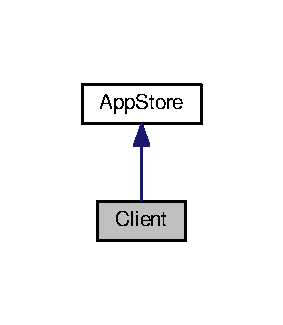
\includegraphics[width=136pt]{class_client__inherit__graph}
\end{center}
\end{figure}


Collaboration diagram for Client\-:
\nopagebreak
\begin{figure}[H]
\begin{center}
\leavevmode
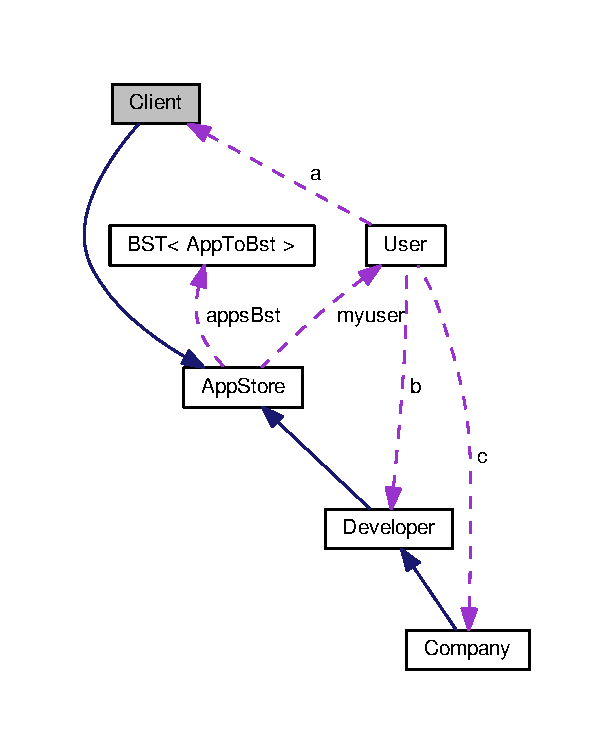
\includegraphics[width=294pt]{class_client__coll__graph}
\end{center}
\end{figure}
\subsection*{Public Member Functions}
\begin{DoxyCompactItemize}
\item 
\hyperlink{class_client_ae51af7aa6b8f591496a8f6a4a87a14bf}{Client} ()
\begin{DoxyCompactList}\small\item\em Creates an object of \hyperlink{class_client}{Client} class. \end{DoxyCompactList}\item 
\hyperlink{class_client_aeb5b0cad9e1c7fa265fa2fc5c8811bb5}{Client} (string n)
\begin{DoxyCompactList}\small\item\em Creates an object of \hyperlink{class_client}{Client} class. \end{DoxyCompactList}\item 
\hyperlink{class_client_a937ad40db78ba6c93e742c593cf63132}{Client} (string u, string p, string n)
\begin{DoxyCompactList}\small\item\em Creates an object of \hyperlink{class_client}{Client} class. \end{DoxyCompactList}\item 
\hyperlink{class_client_a39726efcaba3fa92c1f05aa4b07b6694}{Client} (string user, string pw, string n, float money, vector$<$ \hyperlink{class_app}{App} $\ast$ $>$ v, vector$<$ \hyperlink{structclassification}{classification} $>$ vc)
\begin{DoxyCompactList}\small\item\em Creates an object of \hyperlink{class_client}{Client} class. \end{DoxyCompactList}\item 
string \hyperlink{class_client_a28a677584ad4793b50b31c2e75039e2c}{get\-Name} () const 
\begin{DoxyCompactList}\small\item\em Gets clients name. \end{DoxyCompactList}\item 
string \hyperlink{class_client_a0e00ab51be9a72d8ed059c864fbcc095}{get\-User} () const 
\begin{DoxyCompactList}\small\item\em Gets clients username. \end{DoxyCompactList}\item 
string \hyperlink{class_client_a2a53bedac801f76b39eb2ed3683517a1}{get\-Pw} () const 
\begin{DoxyCompactList}\small\item\em Gets clients password. \end{DoxyCompactList}\item 
void \hyperlink{class_client_ab6e49b98d68f7cf013aaa98076ac04d1}{set\-Username} (string n)
\begin{DoxyCompactList}\small\item\em Sets clients username. \end{DoxyCompactList}\item 
void \hyperlink{class_client_a1feaa7011acc8cb176640e1af2934723}{set\-Name} (string n)
\begin{DoxyCompactList}\small\item\em Sets clients name. \end{DoxyCompactList}\item 
vector$<$ \hyperlink{class_app}{App} $\ast$ $>$ \hyperlink{class_client_a14e9a68136cae4312e98a8330c1d8b7d}{get\-Apps} () const 
\begin{DoxyCompactList}\small\item\em Gets clients apps. \end{DoxyCompactList}\item 
void \hyperlink{class_client_ae23c1978c93d67cfd1b09c94157019eb}{set\-Apps} (vector$<$ \hyperlink{class_app}{App} $\ast$ $>$ v)
\begin{DoxyCompactList}\small\item\em Sets clients apps. \end{DoxyCompactList}\item 
vector$<$ \hyperlink{structclassification}{classification} $>$ \hyperlink{class_client_abd46879af1105932e6363941022f76ce}{get\-Class} () const 
\begin{DoxyCompactList}\small\item\em Gets clients classifications. \end{DoxyCompactList}\item 
void \hyperlink{class_client_a84d1603a7a54058c8c360e2050fc8d10}{set\-Class} (vector$<$ \hyperlink{structclassification}{classification} $>$ c)
\begin{DoxyCompactList}\small\item\em Sets clients classifications. \end{DoxyCompactList}\item 
void \hyperlink{class_client_ae9852558ee40920505015ccf50735e4f}{push\-Back\-App} (\hyperlink{class_app}{App} $\ast$a)
\begin{DoxyCompactList}\small\item\em Puts an \hyperlink{class_app}{App} in the vector. \end{DoxyCompactList}\item 
void \hyperlink{class_client_ac3956ed4b2cc35e3be84ee2e89008108}{add\-To\-Cart} (\hyperlink{class_app}{App} $\ast$a)
\begin{DoxyCompactList}\small\item\em Add to cart. \end{DoxyCompactList}\item 
vector$<$ \hyperlink{class_app}{App} $\ast$ $>$ \hyperlink{class_client_a6f451827c4a1ad44bd80655456fc7b83}{get\-Cart} ()
\begin{DoxyCompactList}\small\item\em Gets clients cart. \end{DoxyCompactList}\item 
int \hyperlink{class_client_aeb4bceecc6d4be3fd53db4d490a0843e}{push\-Back\-Description} (int id, int s, string descripton)
\begin{DoxyCompactList}\small\item\em Puts new description. \end{DoxyCompactList}\item 
void \hyperlink{class_client_ab772fe1ebe3f9782ea8cca34be0adc21}{set\-Pw} (string pw)
\begin{DoxyCompactList}\small\item\em Sets the clients password. \end{DoxyCompactList}\item 
void \hyperlink{class_client_a2538e13b0ef01ecb00a362bb80fdeded}{plus\-Money} (float l)
\begin{DoxyCompactList}\small\item\em Adds money. \end{DoxyCompactList}\item 
float \hyperlink{class_client_ab7273217432f9906a7fd8c50637c6187}{get\-Money} () const 
\begin{DoxyCompactList}\small\item\em Gets the clients money. \end{DoxyCompactList}\item 
void \hyperlink{class_client_a5849a7c952a95fa7d7c941efe4068ade}{set\-Money} (float l)
\begin{DoxyCompactList}\small\item\em Sets clients money. \end{DoxyCompactList}\item 
void \hyperlink{class_client_a9a90dc954556b3f1062900e5df03a201}{erase\-Cart\-App} (int a)
\begin{DoxyCompactList}\small\item\em Erases carts \hyperlink{class_app}{App}. \end{DoxyCompactList}\end{DoxyCompactItemize}
\subsection*{Public Attributes}
\begin{DoxyCompactItemize}
\item 
vector$<$ \hyperlink{class_app}{App} $\ast$ $>$ \hyperlink{class_client_aa3a20b0fa8ebba5e1e7f6826b9b6acff}{cart}
\end{DoxyCompactItemize}


\subsection{Detailed Description}


Definition at line 698 of file app\-Store.\-h.



\subsection{Constructor \& Destructor Documentation}
\hypertarget{class_client_ae51af7aa6b8f591496a8f6a4a87a14bf}{\index{Client@{Client}!Client@{Client}}
\index{Client@{Client}!Client@{Client}}
\subsubsection[{Client}]{\setlength{\rightskip}{0pt plus 5cm}Client\-::\-Client (
\begin{DoxyParamCaption}
{}
\end{DoxyParamCaption}
)}}\label{class_client_ae51af7aa6b8f591496a8f6a4a87a14bf}


Creates an object of \hyperlink{class_client}{Client} class. 



Definition at line 14 of file app\-Store.\-cpp.

\hypertarget{class_client_aeb5b0cad9e1c7fa265fa2fc5c8811bb5}{\index{Client@{Client}!Client@{Client}}
\index{Client@{Client}!Client@{Client}}
\subsubsection[{Client}]{\setlength{\rightskip}{0pt plus 5cm}Client\-::\-Client (
\begin{DoxyParamCaption}
\item[{string}]{n}
\end{DoxyParamCaption}
)}}\label{class_client_aeb5b0cad9e1c7fa265fa2fc5c8811bb5}


Creates an object of \hyperlink{class_client}{Client} class. 


\begin{DoxyParams}{Parameters}
{\em n} & clients name \\
\hline
\end{DoxyParams}


Definition at line 36 of file app\-Store.\-cpp.

\hypertarget{class_client_a937ad40db78ba6c93e742c593cf63132}{\index{Client@{Client}!Client@{Client}}
\index{Client@{Client}!Client@{Client}}
\subsubsection[{Client}]{\setlength{\rightskip}{0pt plus 5cm}Client\-::\-Client (
\begin{DoxyParamCaption}
\item[{string}]{u, }
\item[{string}]{p, }
\item[{string}]{n}
\end{DoxyParamCaption}
)}}\label{class_client_a937ad40db78ba6c93e742c593cf63132}


Creates an object of \hyperlink{class_client}{Client} class. 


\begin{DoxyParams}{Parameters}
{\em u} & username \\
\hline
{\em p} & password \\
\hline
{\em n} & name \\
\hline
\end{DoxyParams}


Definition at line 25 of file app\-Store.\-cpp.

\hypertarget{class_client_a39726efcaba3fa92c1f05aa4b07b6694}{\index{Client@{Client}!Client@{Client}}
\index{Client@{Client}!Client@{Client}}
\subsubsection[{Client}]{\setlength{\rightskip}{0pt plus 5cm}Client\-::\-Client (
\begin{DoxyParamCaption}
\item[{string}]{user, }
\item[{string}]{pw, }
\item[{string}]{n, }
\item[{float}]{money, }
\item[{vector$<$ {\bf App} $\ast$ $>$}]{v, }
\item[{vector$<$ {\bf classification} $>$}]{vc}
\end{DoxyParamCaption}
)}}\label{class_client_a39726efcaba3fa92c1f05aa4b07b6694}


Creates an object of \hyperlink{class_client}{Client} class. 


\begin{DoxyParams}{Parameters}
{\em user} & username of the client \\
\hline
{\em pw} & clients password \\
\hline
{\em n} & clients name \\
\hline
{\em money} & clients actual money \\
\hline
{\em v} & clients apps \\
\hline
{\em vc} & clients classifications \\
\hline
\end{DoxyParams}


Definition at line 47 of file app\-Store.\-cpp.



\subsection{Member Function Documentation}
\hypertarget{class_client_ac3956ed4b2cc35e3be84ee2e89008108}{\index{Client@{Client}!add\-To\-Cart@{add\-To\-Cart}}
\index{add\-To\-Cart@{add\-To\-Cart}!Client@{Client}}
\subsubsection[{add\-To\-Cart}]{\setlength{\rightskip}{0pt plus 5cm}void Client\-::add\-To\-Cart (
\begin{DoxyParamCaption}
\item[{{\bf App} $\ast$}]{a}
\end{DoxyParamCaption}
)}}\label{class_client_ac3956ed4b2cc35e3be84ee2e89008108}


Add to cart. 


\begin{DoxyParams}{Parameters}
{\em $\ast$a} & \hyperlink{class_app}{App} to add \\
\hline
\end{DoxyParams}


Definition at line 128 of file app\-Store.\-cpp.

\hypertarget{class_client_a9a90dc954556b3f1062900e5df03a201}{\index{Client@{Client}!erase\-Cart\-App@{erase\-Cart\-App}}
\index{erase\-Cart\-App@{erase\-Cart\-App}!Client@{Client}}
\subsubsection[{erase\-Cart\-App}]{\setlength{\rightskip}{0pt plus 5cm}void Client\-::erase\-Cart\-App (
\begin{DoxyParamCaption}
\item[{int}]{a}
\end{DoxyParamCaption}
)}}\label{class_client_a9a90dc954556b3f1062900e5df03a201}


Erases carts \hyperlink{class_app}{App}. 


\begin{DoxyParams}{Parameters}
{\em app} & to delete \\
\hline
\end{DoxyParams}


Definition at line 121 of file app\-Store.\-cpp.

\hypertarget{class_client_a14e9a68136cae4312e98a8330c1d8b7d}{\index{Client@{Client}!get\-Apps@{get\-Apps}}
\index{get\-Apps@{get\-Apps}!Client@{Client}}
\subsubsection[{get\-Apps}]{\setlength{\rightskip}{0pt plus 5cm}vector$<$ {\bf App} $\ast$ $>$ Client\-::get\-Apps (
\begin{DoxyParamCaption}
{}
\end{DoxyParamCaption}
) const}}\label{class_client_a14e9a68136cae4312e98a8330c1d8b7d}


Gets clients apps. 

\begin{DoxyReturn}{Returns}
Returns clients apps 
\end{DoxyReturn}


Definition at line 82 of file app\-Store.\-cpp.

\hypertarget{class_client_a6f451827c4a1ad44bd80655456fc7b83}{\index{Client@{Client}!get\-Cart@{get\-Cart}}
\index{get\-Cart@{get\-Cart}!Client@{Client}}
\subsubsection[{get\-Cart}]{\setlength{\rightskip}{0pt plus 5cm}vector$<$ {\bf App} $\ast$ $>$ Client\-::get\-Cart (
\begin{DoxyParamCaption}
{}
\end{DoxyParamCaption}
)}}\label{class_client_a6f451827c4a1ad44bd80655456fc7b83}


Gets clients cart. 

\begin{DoxyReturn}{Returns}
Returns clients cart 
\end{DoxyReturn}


Definition at line 131 of file app\-Store.\-cpp.

\hypertarget{class_client_abd46879af1105932e6363941022f76ce}{\index{Client@{Client}!get\-Class@{get\-Class}}
\index{get\-Class@{get\-Class}!Client@{Client}}
\subsubsection[{get\-Class}]{\setlength{\rightskip}{0pt plus 5cm}vector$<$ {\bf classification} $>$ Client\-::get\-Class (
\begin{DoxyParamCaption}
{}
\end{DoxyParamCaption}
) const}}\label{class_client_abd46879af1105932e6363941022f76ce}


Gets clients classifications. 

\begin{DoxyReturn}{Returns}
Returns clients classifications 
\end{DoxyReturn}


Definition at line 90 of file app\-Store.\-cpp.

\hypertarget{class_client_ab7273217432f9906a7fd8c50637c6187}{\index{Client@{Client}!get\-Money@{get\-Money}}
\index{get\-Money@{get\-Money}!Client@{Client}}
\subsubsection[{get\-Money}]{\setlength{\rightskip}{0pt plus 5cm}float Client\-::get\-Money (
\begin{DoxyParamCaption}
{}
\end{DoxyParamCaption}
) const}}\label{class_client_ab7273217432f9906a7fd8c50637c6187}


Gets the clients money. 

\begin{DoxyReturn}{Returns}
Returns clients money 
\end{DoxyReturn}


Definition at line 74 of file app\-Store.\-cpp.

\hypertarget{class_client_a28a677584ad4793b50b31c2e75039e2c}{\index{Client@{Client}!get\-Name@{get\-Name}}
\index{get\-Name@{get\-Name}!Client@{Client}}
\subsubsection[{get\-Name}]{\setlength{\rightskip}{0pt plus 5cm}string Client\-::get\-Name (
\begin{DoxyParamCaption}
{}
\end{DoxyParamCaption}
) const}}\label{class_client_a28a677584ad4793b50b31c2e75039e2c}


Gets clients name. 

\begin{DoxyReturn}{Returns}
Returns clients name 
\end{DoxyReturn}


Definition at line 58 of file app\-Store.\-cpp.

\hypertarget{class_client_a2a53bedac801f76b39eb2ed3683517a1}{\index{Client@{Client}!get\-Pw@{get\-Pw}}
\index{get\-Pw@{get\-Pw}!Client@{Client}}
\subsubsection[{get\-Pw}]{\setlength{\rightskip}{0pt plus 5cm}string Client\-::get\-Pw (
\begin{DoxyParamCaption}
{}
\end{DoxyParamCaption}
) const}}\label{class_client_a2a53bedac801f76b39eb2ed3683517a1}


Gets clients password. 

\begin{DoxyReturn}{Returns}
Returns clients password 
\end{DoxyReturn}


Definition at line 102 of file app\-Store.\-cpp.

\hypertarget{class_client_a0e00ab51be9a72d8ed059c864fbcc095}{\index{Client@{Client}!get\-User@{get\-User}}
\index{get\-User@{get\-User}!Client@{Client}}
\subsubsection[{get\-User}]{\setlength{\rightskip}{0pt plus 5cm}string Client\-::get\-User (
\begin{DoxyParamCaption}
{}
\end{DoxyParamCaption}
) const}}\label{class_client_a0e00ab51be9a72d8ed059c864fbcc095}


Gets clients username. 

\begin{DoxyReturn}{Returns}
Returns clients username 
\end{DoxyReturn}


Definition at line 98 of file app\-Store.\-cpp.

\hypertarget{class_client_a2538e13b0ef01ecb00a362bb80fdeded}{\index{Client@{Client}!plus\-Money@{plus\-Money}}
\index{plus\-Money@{plus\-Money}!Client@{Client}}
\subsubsection[{plus\-Money}]{\setlength{\rightskip}{0pt plus 5cm}void Client\-::plus\-Money (
\begin{DoxyParamCaption}
\item[{float}]{l}
\end{DoxyParamCaption}
)}}\label{class_client_a2538e13b0ef01ecb00a362bb80fdeded}


Adds money. 


\begin{DoxyParams}{Parameters}
{\em l} & money to add \\
\hline
\end{DoxyParams}


Definition at line 70 of file app\-Store.\-cpp.

\hypertarget{class_client_ae9852558ee40920505015ccf50735e4f}{\index{Client@{Client}!push\-Back\-App@{push\-Back\-App}}
\index{push\-Back\-App@{push\-Back\-App}!Client@{Client}}
\subsubsection[{push\-Back\-App}]{\setlength{\rightskip}{0pt plus 5cm}void Client\-::push\-Back\-App (
\begin{DoxyParamCaption}
\item[{{\bf App} $\ast$}]{a}
\end{DoxyParamCaption}
)}}\label{class_client_ae9852558ee40920505015ccf50735e4f}


Puts an \hyperlink{class_app}{App} in the vector. 


\begin{DoxyParams}{Parameters}
{\em $\ast$a} & \hyperlink{class_app}{App} to insert \\
\hline
\end{DoxyParams}


Definition at line 106 of file app\-Store.\-cpp.

\hypertarget{class_client_aeb4bceecc6d4be3fd53db4d490a0843e}{\index{Client@{Client}!push\-Back\-Description@{push\-Back\-Description}}
\index{push\-Back\-Description@{push\-Back\-Description}!Client@{Client}}
\subsubsection[{push\-Back\-Description}]{\setlength{\rightskip}{0pt plus 5cm}int Client\-::push\-Back\-Description (
\begin{DoxyParamCaption}
\item[{int}]{id, }
\item[{int}]{s, }
\item[{string}]{descripton}
\end{DoxyParamCaption}
)}}\label{class_client_aeb4bceecc6d4be3fd53db4d490a0843e}


Puts new description. 


\begin{DoxyParams}{Parameters}
{\em id} & Id of the app to describe \\
\hline
{\em s} & Stars given by the client \\
\hline
{\em description} & new description of the client\\
\hline
\end{DoxyParams}
\begin{DoxyReturn}{Returns}
1 
\end{DoxyReturn}


Definition at line 110 of file app\-Store.\-cpp.

\hypertarget{class_client_ae23c1978c93d67cfd1b09c94157019eb}{\index{Client@{Client}!set\-Apps@{set\-Apps}}
\index{set\-Apps@{set\-Apps}!Client@{Client}}
\subsubsection[{set\-Apps}]{\setlength{\rightskip}{0pt plus 5cm}void Client\-::set\-Apps (
\begin{DoxyParamCaption}
\item[{vector$<$ {\bf App} $\ast$ $>$}]{v}
\end{DoxyParamCaption}
)}}\label{class_client_ae23c1978c93d67cfd1b09c94157019eb}


Sets clients apps. 


\begin{DoxyParams}{Parameters}
{\em Apps} & to set \\
\hline
\end{DoxyParams}


Definition at line 86 of file app\-Store.\-cpp.

\hypertarget{class_client_a84d1603a7a54058c8c360e2050fc8d10}{\index{Client@{Client}!set\-Class@{set\-Class}}
\index{set\-Class@{set\-Class}!Client@{Client}}
\subsubsection[{set\-Class}]{\setlength{\rightskip}{0pt plus 5cm}void Client\-::set\-Class (
\begin{DoxyParamCaption}
\item[{vector$<$ {\bf classification} $>$}]{c}
\end{DoxyParamCaption}
)}}\label{class_client_a84d1603a7a54058c8c360e2050fc8d10}


Sets clients classifications. 


\begin{DoxyParams}{Parameters}
{\em c} & clients classifications to set \\
\hline
\end{DoxyParams}


Definition at line 94 of file app\-Store.\-cpp.

\hypertarget{class_client_a5849a7c952a95fa7d7c941efe4068ade}{\index{Client@{Client}!set\-Money@{set\-Money}}
\index{set\-Money@{set\-Money}!Client@{Client}}
\subsubsection[{set\-Money}]{\setlength{\rightskip}{0pt plus 5cm}void Client\-::set\-Money (
\begin{DoxyParamCaption}
\item[{float}]{l}
\end{DoxyParamCaption}
)}}\label{class_client_a5849a7c952a95fa7d7c941efe4068ade}


Sets clients money. 


\begin{DoxyParams}{Parameters}
{\em l} & money to be set \\
\hline
\end{DoxyParams}


Definition at line 78 of file app\-Store.\-cpp.

\hypertarget{class_client_a1feaa7011acc8cb176640e1af2934723}{\index{Client@{Client}!set\-Name@{set\-Name}}
\index{set\-Name@{set\-Name}!Client@{Client}}
\subsubsection[{set\-Name}]{\setlength{\rightskip}{0pt plus 5cm}void Client\-::set\-Name (
\begin{DoxyParamCaption}
\item[{string}]{n}
\end{DoxyParamCaption}
)}}\label{class_client_a1feaa7011acc8cb176640e1af2934723}


Sets clients name. 


\begin{DoxyParams}{Parameters}
{\em n} & clients name \\
\hline
\end{DoxyParams}


Definition at line 62 of file app\-Store.\-cpp.

\hypertarget{class_client_ab772fe1ebe3f9782ea8cca34be0adc21}{\index{Client@{Client}!set\-Pw@{set\-Pw}}
\index{set\-Pw@{set\-Pw}!Client@{Client}}
\subsubsection[{set\-Pw}]{\setlength{\rightskip}{0pt plus 5cm}void Client\-::set\-Pw (
\begin{DoxyParamCaption}
\item[{string}]{pw}
\end{DoxyParamCaption}
)}}\label{class_client_ab772fe1ebe3f9782ea8cca34be0adc21}


Sets the clients password. 


\begin{DoxyParams}{Parameters}
{\em Password} & to set \\
\hline
\end{DoxyParams}


Definition at line 124 of file app\-Store.\-cpp.

\hypertarget{class_client_ab6e49b98d68f7cf013aaa98076ac04d1}{\index{Client@{Client}!set\-Username@{set\-Username}}
\index{set\-Username@{set\-Username}!Client@{Client}}
\subsubsection[{set\-Username}]{\setlength{\rightskip}{0pt plus 5cm}void Client\-::set\-Username (
\begin{DoxyParamCaption}
\item[{string}]{n}
\end{DoxyParamCaption}
)}}\label{class_client_ab6e49b98d68f7cf013aaa98076ac04d1}


Sets clients username. 


\begin{DoxyParams}{Parameters}
{\em n} & clients username \\
\hline
\end{DoxyParams}


Definition at line 66 of file app\-Store.\-cpp.



\subsection{Member Data Documentation}
\hypertarget{class_client_aa3a20b0fa8ebba5e1e7f6826b9b6acff}{\index{Client@{Client}!cart@{cart}}
\index{cart@{cart}!Client@{Client}}
\subsubsection[{cart}]{\setlength{\rightskip}{0pt plus 5cm}vector$<${\bf App}$\ast$$>$ Client\-::cart}}\label{class_client_aa3a20b0fa8ebba5e1e7f6826b9b6acff}


Definition at line 706 of file app\-Store.\-h.



The documentation for this class was generated from the following files\-:\begin{DoxyCompactItemize}
\item 
src/\hyperlink{app_store_8h}{app\-Store.\-h}\item 
src/\hyperlink{app_store_8cpp}{app\-Store.\-cpp}\end{DoxyCompactItemize}

\hypertarget{class_client_not_found}{\section{Client\-Not\-Found Class Reference}
\label{class_client_not_found}\index{Client\-Not\-Found@{Client\-Not\-Found}}
}


{\ttfamily \#include $<$app\-Store.\-h$>$}

\subsection*{Public Member Functions}
\begin{DoxyCompactItemize}
\item 
\hyperlink{class_client_not_found_a8d279d0c09d16873ed48a42b4236b649}{Client\-Not\-Found} (string n)
\begin{DoxyCompactList}\small\item\em Creates an objecto (exception) of class \hyperlink{class_client_not_found}{Client\-Not\-Found}. \end{DoxyCompactList}\item 
string \hyperlink{class_client_not_found_a2c58b452f022fa6ecb13000485a79e1e}{retname} ()
\end{DoxyCompactItemize}
\subsection*{Public Attributes}
\begin{DoxyCompactItemize}
\item 
string \hyperlink{class_client_not_found_a1930a4407c0c37ede93d7dcc73552114}{name}
\end{DoxyCompactItemize}


\subsection{Detailed Description}


Definition at line 1103 of file app\-Store.\-h.



\subsection{Constructor \& Destructor Documentation}
\hypertarget{class_client_not_found_a8d279d0c09d16873ed48a42b4236b649}{\index{Client\-Not\-Found@{Client\-Not\-Found}!Client\-Not\-Found@{Client\-Not\-Found}}
\index{Client\-Not\-Found@{Client\-Not\-Found}!ClientNotFound@{Client\-Not\-Found}}
\subsubsection[{Client\-Not\-Found}]{\setlength{\rightskip}{0pt plus 5cm}Client\-Not\-Found\-::\-Client\-Not\-Found (
\begin{DoxyParamCaption}
\item[{string}]{n}
\end{DoxyParamCaption}
)\hspace{0.3cm}{\ttfamily [inline]}}}\label{class_client_not_found_a8d279d0c09d16873ed48a42b4236b649}


Creates an objecto (exception) of class \hyperlink{class_client_not_found}{Client\-Not\-Found}. 


\begin{DoxyParams}{Parameters}
{\em n} & name \\
\hline
\end{DoxyParams}


Definition at line 1111 of file app\-Store.\-h.



\subsection{Member Function Documentation}
\hypertarget{class_client_not_found_a2c58b452f022fa6ecb13000485a79e1e}{\index{Client\-Not\-Found@{Client\-Not\-Found}!retname@{retname}}
\index{retname@{retname}!ClientNotFound@{Client\-Not\-Found}}
\subsubsection[{retname}]{\setlength{\rightskip}{0pt plus 5cm}string Client\-Not\-Found\-::retname (
\begin{DoxyParamCaption}
{}
\end{DoxyParamCaption}
)\hspace{0.3cm}{\ttfamily [inline]}}}\label{class_client_not_found_a2c58b452f022fa6ecb13000485a79e1e}


Definition at line 1114 of file app\-Store.\-h.



\subsection{Member Data Documentation}
\hypertarget{class_client_not_found_a1930a4407c0c37ede93d7dcc73552114}{\index{Client\-Not\-Found@{Client\-Not\-Found}!name@{name}}
\index{name@{name}!ClientNotFound@{Client\-Not\-Found}}
\subsubsection[{name}]{\setlength{\rightskip}{0pt plus 5cm}string Client\-Not\-Found\-::name}}\label{class_client_not_found_a1930a4407c0c37ede93d7dcc73552114}


Definition at line 1105 of file app\-Store.\-h.



The documentation for this class was generated from the following file\-:\begin{DoxyCompactItemize}
\item 
src/\hyperlink{app_store_8h}{app\-Store.\-h}\end{DoxyCompactItemize}

\hypertarget{class_company}{\section{Company Class Reference}
\label{class_company}\index{Company@{Company}}
}


{\ttfamily \#include $<$app\-Store.\-h$>$}



Inheritance diagram for Company\-:
\nopagebreak
\begin{figure}[H]
\begin{center}
\leavevmode
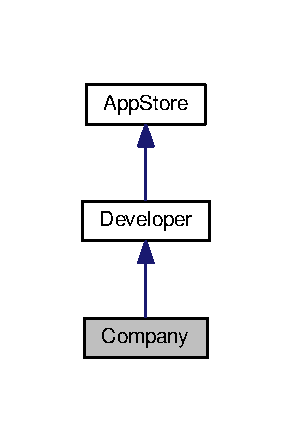
\includegraphics[width=140pt]{class_company__inherit__graph}
\end{center}
\end{figure}


Collaboration diagram for Company\-:
\nopagebreak
\begin{figure}[H]
\begin{center}
\leavevmode
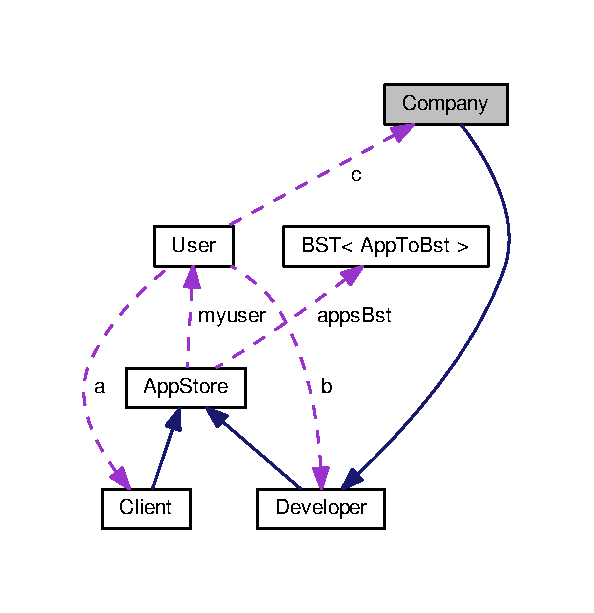
\includegraphics[width=285pt]{class_company__coll__graph}
\end{center}
\end{figure}
\subsection*{Public Member Functions}
\begin{DoxyCompactItemize}
\item 
\hyperlink{class_company_a29937dda711b09df306ae7ca9b3d6b42}{Company} ()
\begin{DoxyCompactList}\small\item\em creates an object of class \hyperlink{class_company}{Company} \end{DoxyCompactList}\item 
\hyperlink{class_company_af668b01e0be2b4472dbc443fb1e39e51}{Company} (string username, string password, string name, string address, int nif)
\begin{DoxyCompactList}\small\item\em creates an object of class \hyperlink{class_company}{Company} \end{DoxyCompactList}\item 
\hyperlink{class_company_a1f0fd388082b43b5779c5119ce5a04f8}{Company} (string username, string password, string n, string a, float m, int nif, vector$<$ \hyperlink{class_app}{App} $\ast$ $>$ v)
\begin{DoxyCompactList}\small\item\em creates an object of class \hyperlink{class_company}{Company} \end{DoxyCompactList}\item 
string \hyperlink{class_company_a9b62ad43569259771a2d4be5fb2c9255}{get\-Official\-Name} () const 
\begin{DoxyCompactList}\small\item\em Gets the official name. \end{DoxyCompactList}\item 
void \hyperlink{class_company_aa0a41e16db04009dea627e148bbb1467}{set\-Official\-Name} (string ofn)
\begin{DoxyCompactList}\small\item\em sets the official name \end{DoxyCompactList}\item 
int \hyperlink{class_company_a9bd541b695636b65637a34b209d6537f}{get\-Nif} () const 
\begin{DoxyCompactList}\small\item\em gets the official name \end{DoxyCompactList}\item 
void \hyperlink{class_company_abec6540c99b8f01ee7a63d229e364868}{set\-Nif} (int n)
\begin{DoxyCompactList}\small\item\em sets the nif \end{DoxyCompactList}\end{DoxyCompactItemize}
\subsection*{Additional Inherited Members}


\subsection{Detailed Description}


Definition at line 965 of file app\-Store.\-h.



\subsection{Constructor \& Destructor Documentation}
\hypertarget{class_company_a29937dda711b09df306ae7ca9b3d6b42}{\index{Company@{Company}!Company@{Company}}
\index{Company@{Company}!Company@{Company}}
\subsubsection[{Company}]{\setlength{\rightskip}{0pt plus 5cm}Company\-::\-Company (
\begin{DoxyParamCaption}
{}
\end{DoxyParamCaption}
)}}\label{class_company_a29937dda711b09df306ae7ca9b3d6b42}


creates an object of class \hyperlink{class_company}{Company} 



Definition at line 310 of file app\-Store.\-cpp.

\hypertarget{class_company_af668b01e0be2b4472dbc443fb1e39e51}{\index{Company@{Company}!Company@{Company}}
\index{Company@{Company}!Company@{Company}}
\subsubsection[{Company}]{\setlength{\rightskip}{0pt plus 5cm}Company\-::\-Company (
\begin{DoxyParamCaption}
\item[{string}]{username, }
\item[{string}]{password, }
\item[{string}]{name, }
\item[{string}]{address, }
\item[{int}]{nif}
\end{DoxyParamCaption}
)}}\label{class_company_af668b01e0be2b4472dbc443fb1e39e51}


creates an object of class \hyperlink{class_company}{Company} 


\begin{DoxyParams}{Parameters}
{\em username} & \\
\hline
{\em password} & \\
\hline
{\em name} & \\
\hline
{\em address} & \\
\hline
{\em nif} & \\
\hline
\end{DoxyParams}


Definition at line 318 of file app\-Store.\-cpp.

\hypertarget{class_company_a1f0fd388082b43b5779c5119ce5a04f8}{\index{Company@{Company}!Company@{Company}}
\index{Company@{Company}!Company@{Company}}
\subsubsection[{Company}]{\setlength{\rightskip}{0pt plus 5cm}Company\-::\-Company (
\begin{DoxyParamCaption}
\item[{string}]{username, }
\item[{string}]{password, }
\item[{string}]{n, }
\item[{string}]{a, }
\item[{float}]{m, }
\item[{int}]{nif, }
\item[{vector$<$ {\bf App} $\ast$ $>$}]{v}
\end{DoxyParamCaption}
)}}\label{class_company_a1f0fd388082b43b5779c5119ce5a04f8}


creates an object of class \hyperlink{class_company}{Company} 


\begin{DoxyParams}{Parameters}
{\em username} & username of the buyer \\
\hline
{\em password} & of the user \\
\hline
{\em n} & name of the user \\
\hline
{\em a} & address of the user \\
\hline
{\em m} & money of the user \\
\hline
{\em nif} & \\
\hline
{\em v} & apps of the user \\
\hline
\end{DoxyParams}


Definition at line 313 of file app\-Store.\-cpp.



\subsection{Member Function Documentation}
\hypertarget{class_company_a9bd541b695636b65637a34b209d6537f}{\index{Company@{Company}!get\-Nif@{get\-Nif}}
\index{get\-Nif@{get\-Nif}!Company@{Company}}
\subsubsection[{get\-Nif}]{\setlength{\rightskip}{0pt plus 5cm}int Company\-::get\-Nif (
\begin{DoxyParamCaption}
{}
\end{DoxyParamCaption}
) const}}\label{class_company_a9bd541b695636b65637a34b209d6537f}


gets the official name 

\begin{DoxyReturn}{Returns}
official name 
\end{DoxyReturn}


Definition at line 323 of file app\-Store.\-cpp.

\hypertarget{class_company_a9b62ad43569259771a2d4be5fb2c9255}{\index{Company@{Company}!get\-Official\-Name@{get\-Official\-Name}}
\index{get\-Official\-Name@{get\-Official\-Name}!Company@{Company}}
\subsubsection[{get\-Official\-Name}]{\setlength{\rightskip}{0pt plus 5cm}string Company\-::get\-Official\-Name (
\begin{DoxyParamCaption}
{}
\end{DoxyParamCaption}
) const}}\label{class_company_a9b62ad43569259771a2d4be5fb2c9255}


Gets the official name. 

\begin{DoxyReturn}{Returns}
returns the official name 
\end{DoxyReturn}
\hypertarget{class_company_abec6540c99b8f01ee7a63d229e364868}{\index{Company@{Company}!set\-Nif@{set\-Nif}}
\index{set\-Nif@{set\-Nif}!Company@{Company}}
\subsubsection[{set\-Nif}]{\setlength{\rightskip}{0pt plus 5cm}void Company\-::set\-Nif (
\begin{DoxyParamCaption}
\item[{int}]{n}
\end{DoxyParamCaption}
)}}\label{class_company_abec6540c99b8f01ee7a63d229e364868}


sets the nif 


\begin{DoxyParams}{Parameters}
{\em nif} & \\
\hline
\end{DoxyParams}


Definition at line 327 of file app\-Store.\-cpp.

\hypertarget{class_company_aa0a41e16db04009dea627e148bbb1467}{\index{Company@{Company}!set\-Official\-Name@{set\-Official\-Name}}
\index{set\-Official\-Name@{set\-Official\-Name}!Company@{Company}}
\subsubsection[{set\-Official\-Name}]{\setlength{\rightskip}{0pt plus 5cm}void Company\-::set\-Official\-Name (
\begin{DoxyParamCaption}
\item[{string}]{ofn}
\end{DoxyParamCaption}
)}}\label{class_company_aa0a41e16db04009dea627e148bbb1467}


sets the official name 


\begin{DoxyParams}{Parameters}
{\em ofn} & official name \\
\hline
\end{DoxyParams}


The documentation for this class was generated from the following files\-:\begin{DoxyCompactItemize}
\item 
src/\hyperlink{app_store_8h}{app\-Store.\-h}\item 
src/\hyperlink{app_store_8cpp}{app\-Store.\-cpp}\end{DoxyCompactItemize}

\hypertarget{struct_date}{\section{Date Struct Reference}
\label{struct_date}\index{Date@{Date}}
}


{\ttfamily \#include $<$app\-Store.\-h$>$}

\subsection*{Public Member Functions}
\begin{DoxyCompactItemize}
\item 
\hyperlink{struct_date_a4e59ed4ba66eec61c27460c5d09fa1bd}{Date} ()
\begin{DoxyCompactList}\small\item\em Creates a date class object. \end{DoxyCompactList}\item 
\hyperlink{struct_date_a6035b37cfccaf63b33f6c0e95b0099ea}{Date} (int h, int mi, int d, int m, int y)
\begin{DoxyCompactList}\small\item\em Creates a date class object. \end{DoxyCompactList}\item 
bool \hyperlink{struct_date_a6ec06696ab11aba7f7b0c3586a13a212}{operator$<$} (\hyperlink{struct_date}{Date} const \&b) const 
\begin{DoxyCompactList}\small\item\em Operator $<$ overload. \end{DoxyCompactList}\item 
bool \hyperlink{struct_date_ad3f9054d9708aa97b237ddf88495d70f}{operator$>$} (\hyperlink{struct_date}{Date} const \&b) const 
\begin{DoxyCompactList}\small\item\em Operator $>$ overload. \end{DoxyCompactList}\item 
bool \hyperlink{struct_date_af7d714167e08de849d2d04b2246cfcfa}{operator==} (\hyperlink{struct_date}{Date} const \&b) const 
\begin{DoxyCompactList}\small\item\em Operator == overload. \end{DoxyCompactList}\end{DoxyCompactItemize}
\subsection*{Public Attributes}
\begin{DoxyCompactItemize}
\item 
int \hyperlink{struct_date_a59f93395dbec8ce9945f2ea091250c42}{hour}
\item 
int \hyperlink{struct_date_a3bd2b03da68ad8995b56a393a0c4f4a0}{minutes}
\item 
int \hyperlink{struct_date_a5b192adcabf2b2871e3f0b76c1ec1601}{day}
\item 
int \hyperlink{struct_date_a533843e07c6ac8d19fee9b16f5336ba2}{month}
\item 
int \hyperlink{struct_date_a3eeced2ed56bc95d56782b9e738db8ea}{year}
\end{DoxyCompactItemize}


\subsection{Detailed Description}


Definition at line 442 of file app\-Store.\-h.



\subsection{Constructor \& Destructor Documentation}
\hypertarget{struct_date_a4e59ed4ba66eec61c27460c5d09fa1bd}{\index{Date@{Date}!Date@{Date}}
\index{Date@{Date}!Date@{Date}}
\subsubsection[{Date}]{\setlength{\rightskip}{0pt plus 5cm}Date\-::\-Date (
\begin{DoxyParamCaption}
{}
\end{DoxyParamCaption}
)}}\label{struct_date_a4e59ed4ba66eec61c27460c5d09fa1bd}


Creates a date class object. 



Definition at line 333 of file app\-Store.\-cpp.

\hypertarget{struct_date_a6035b37cfccaf63b33f6c0e95b0099ea}{\index{Date@{Date}!Date@{Date}}
\index{Date@{Date}!Date@{Date}}
\subsubsection[{Date}]{\setlength{\rightskip}{0pt plus 5cm}Date\-::\-Date (
\begin{DoxyParamCaption}
\item[{int}]{h, }
\item[{int}]{mi, }
\item[{int}]{d, }
\item[{int}]{m, }
\item[{int}]{y}
\end{DoxyParamCaption}
)}}\label{struct_date_a6035b37cfccaf63b33f6c0e95b0099ea}


Creates a date class object. 


\begin{DoxyParams}{Parameters}
{\em h} & hours \\
\hline
{\em mi} & minutes \\
\hline
{\em d} & day \\
\hline
{\em m} & month \\
\hline
{\em y} & year \\
\hline
\end{DoxyParams}


Definition at line 343 of file app\-Store.\-cpp.



\subsection{Member Function Documentation}
\hypertarget{struct_date_a6ec06696ab11aba7f7b0c3586a13a212}{\index{Date@{Date}!operator$<$@{operator$<$}}
\index{operator$<$@{operator$<$}!Date@{Date}}
\subsubsection[{operator$<$}]{\setlength{\rightskip}{0pt plus 5cm}bool Date\-::operator$<$ (
\begin{DoxyParamCaption}
\item[{{\bf Date} const \&}]{b}
\end{DoxyParamCaption}
) const}}\label{struct_date_a6ec06696ab11aba7f7b0c3586a13a212}


Operator $<$ overload. 


\begin{DoxyParams}{Parameters}
{\em \hyperlink{struct_date}{Date}} & structure\\
\hline
\end{DoxyParams}
\begin{DoxyReturn}{Returns}
Returns true if $<$ 
\end{DoxyReturn}


Definition at line 351 of file app\-Store.\-cpp.

\hypertarget{struct_date_af7d714167e08de849d2d04b2246cfcfa}{\index{Date@{Date}!operator==@{operator==}}
\index{operator==@{operator==}!Date@{Date}}
\subsubsection[{operator==}]{\setlength{\rightskip}{0pt plus 5cm}bool Date\-::operator== (
\begin{DoxyParamCaption}
\item[{{\bf Date} const \&}]{b}
\end{DoxyParamCaption}
) const}}\label{struct_date_af7d714167e08de849d2d04b2246cfcfa}


Operator == overload. 


\begin{DoxyParams}{Parameters}
{\em \hyperlink{struct_date}{Date}} & structure\\
\hline
\end{DoxyParams}
\begin{DoxyReturn}{Returns}
Returns true if == 
\end{DoxyReturn}


Definition at line 398 of file app\-Store.\-cpp.

\hypertarget{struct_date_ad3f9054d9708aa97b237ddf88495d70f}{\index{Date@{Date}!operator$>$@{operator$>$}}
\index{operator$>$@{operator$>$}!Date@{Date}}
\subsubsection[{operator$>$}]{\setlength{\rightskip}{0pt plus 5cm}bool Date\-::operator$>$ (
\begin{DoxyParamCaption}
\item[{{\bf Date} const \&}]{b}
\end{DoxyParamCaption}
) const}}\label{struct_date_ad3f9054d9708aa97b237ddf88495d70f}


Operator $>$ overload. 


\begin{DoxyParams}{Parameters}
{\em \hyperlink{struct_date}{Date}} & structure\\
\hline
\end{DoxyParams}
\begin{DoxyReturn}{Returns}
Returns true if $>$ 
\end{DoxyReturn}


Definition at line 374 of file app\-Store.\-cpp.



\subsection{Member Data Documentation}
\hypertarget{struct_date_a5b192adcabf2b2871e3f0b76c1ec1601}{\index{Date@{Date}!day@{day}}
\index{day@{day}!Date@{Date}}
\subsubsection[{day}]{\setlength{\rightskip}{0pt plus 5cm}int Date\-::day}}\label{struct_date_a5b192adcabf2b2871e3f0b76c1ec1601}


Definition at line 445 of file app\-Store.\-h.

\hypertarget{struct_date_a59f93395dbec8ce9945f2ea091250c42}{\index{Date@{Date}!hour@{hour}}
\index{hour@{hour}!Date@{Date}}
\subsubsection[{hour}]{\setlength{\rightskip}{0pt plus 5cm}int Date\-::hour}}\label{struct_date_a59f93395dbec8ce9945f2ea091250c42}


Definition at line 443 of file app\-Store.\-h.

\hypertarget{struct_date_a3bd2b03da68ad8995b56a393a0c4f4a0}{\index{Date@{Date}!minutes@{minutes}}
\index{minutes@{minutes}!Date@{Date}}
\subsubsection[{minutes}]{\setlength{\rightskip}{0pt plus 5cm}int Date\-::minutes}}\label{struct_date_a3bd2b03da68ad8995b56a393a0c4f4a0}


Definition at line 444 of file app\-Store.\-h.

\hypertarget{struct_date_a533843e07c6ac8d19fee9b16f5336ba2}{\index{Date@{Date}!month@{month}}
\index{month@{month}!Date@{Date}}
\subsubsection[{month}]{\setlength{\rightskip}{0pt plus 5cm}int Date\-::month}}\label{struct_date_a533843e07c6ac8d19fee9b16f5336ba2}


Definition at line 446 of file app\-Store.\-h.

\hypertarget{struct_date_a3eeced2ed56bc95d56782b9e738db8ea}{\index{Date@{Date}!year@{year}}
\index{year@{year}!Date@{Date}}
\subsubsection[{year}]{\setlength{\rightskip}{0pt plus 5cm}int Date\-::year}}\label{struct_date_a3eeced2ed56bc95d56782b9e738db8ea}


Definition at line 447 of file app\-Store.\-h.



The documentation for this struct was generated from the following files\-:\begin{DoxyCompactItemize}
\item 
src/\hyperlink{app_store_8h}{app\-Store.\-h}\item 
src/\hyperlink{app_store_8cpp}{app\-Store.\-cpp}\end{DoxyCompactItemize}

\hypertarget{class_developer}{\section{Developer Class Reference}
\label{class_developer}\index{Developer@{Developer}}
}


{\ttfamily \#include $<$app\-Store.\-h$>$}



Inheritance diagram for Developer\-:
\nopagebreak
\begin{figure}[H]
\begin{center}
\leavevmode
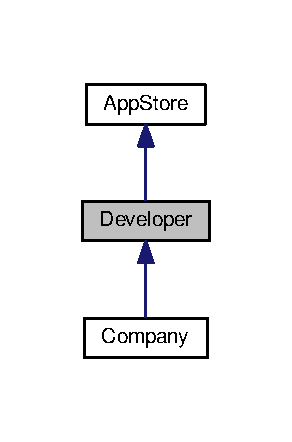
\includegraphics[width=140pt]{class_developer__inherit__graph}
\end{center}
\end{figure}


Collaboration diagram for Developer\-:
\nopagebreak
\begin{figure}[H]
\begin{center}
\leavevmode
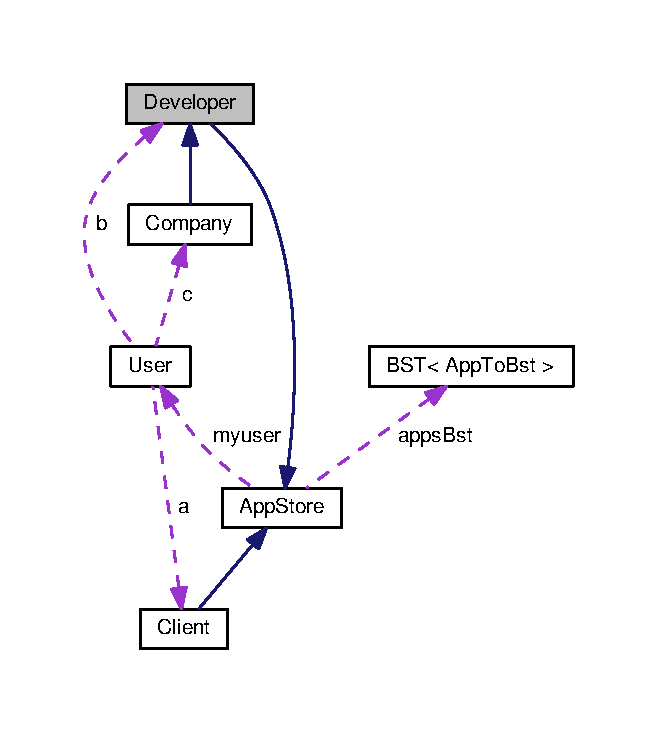
\includegraphics[width=314pt]{class_developer__coll__graph}
\end{center}
\end{figure}
\subsection*{Public Member Functions}
\begin{DoxyCompactItemize}
\item 
\hyperlink{class_developer_a1acf937b03598b68b93c010bfc90f702}{Developer} ()
\begin{DoxyCompactList}\small\item\em Creates an object of class \hyperlink{class_developer}{Developer}. \end{DoxyCompactList}\item 
\hyperlink{class_developer_a9e6851b29e5e3eddb65d3fead20fcc11}{Developer} (string n, string a)
\begin{DoxyCompactList}\small\item\em Creates an object of class \hyperlink{class_developer}{Developer}. \end{DoxyCompactList}\item 
\hyperlink{class_developer_a566bc9559532a39eb343bae605d81dbb}{Developer} (string username, string password, string n, string a, float m, vector$<$ \hyperlink{class_app}{App} $\ast$ $>$ v)
\begin{DoxyCompactList}\small\item\em Creates an object of class \hyperlink{class_developer}{Developer}. \end{DoxyCompactList}\item 
\hyperlink{class_developer_a22955164da669fdfb4e2993031c7ac3b}{Developer} (string username, string password, string n, string a)
\begin{DoxyCompactList}\small\item\em Creates an object of class \hyperlink{class_developer}{Developer}. \end{DoxyCompactList}\item 
string \hyperlink{class_developer_ab596fa3410bc9ec868ae57cf81461ce7}{get\-Name} () const 
\begin{DoxyCompactList}\small\item\em Gets the name of the developer. \end{DoxyCompactList}\item 
void \hyperlink{class_developer_a98717ed7e5e6f72e24ec49d210c2e086}{set\-Name} (string n)
\begin{DoxyCompactList}\small\item\em Sets the name of the developer. \end{DoxyCompactList}\item 
string \hyperlink{class_developer_ab4e0bd9ec4a725ea0074686f624a4dd5}{get\-Address} () const 
\begin{DoxyCompactList}\small\item\em Gets the address of the developer. \end{DoxyCompactList}\item 
void \hyperlink{class_developer_a9c360469be382413d32f4e08b9123bb9}{set\-Address} (string ad)
\begin{DoxyCompactList}\small\item\em Sets the address of the developer. \end{DoxyCompactList}\item 
string \hyperlink{class_developer_a81bc87b5c918165049dcf71f3e4cd883}{get\-User} () const 
\begin{DoxyCompactList}\small\item\em Gets the username of the developer. \end{DoxyCompactList}\item 
string \hyperlink{class_developer_a1b66c4f606291cc4f4d7a5a6aa1c737b}{get\-Pw} () const 
\begin{DoxyCompactList}\small\item\em Gets the password of the developer. \end{DoxyCompactList}\item 
vector$<$ \hyperlink{class_app}{App} $\ast$ $>$ \hyperlink{class_developer_a9a9569dd9320e5a5637ccd3bc870acec}{get\-Apps} () const 
\begin{DoxyCompactList}\small\item\em Gets the Apps of the developer. \end{DoxyCompactList}\item 
void \hyperlink{class_developer_ac2d1dd070fc88aae2e5e86e0be192615}{set\-Apps} (vector$<$ \hyperlink{class_app}{App} $\ast$ $>$ v)
\begin{DoxyCompactList}\small\item\em Sets the Apps of the developer. \end{DoxyCompactList}\item 
void \hyperlink{class_developer_ab121efa005a8a7b878408ad65a269dd6}{set\-Pw} (string pw)
\begin{DoxyCompactList}\small\item\em Sets the password of the developer. \end{DoxyCompactList}\item 
void \hyperlink{class_developer_a41a32e1735afeb1422090fd11f8dd5dd}{set\-Username} (string n)
\begin{DoxyCompactList}\small\item\em Sets the username of the developer. \end{DoxyCompactList}\item 
float \hyperlink{class_developer_aee320cff50fb96e15451a5b2ceb18b99}{get\-Money} () const 
\begin{DoxyCompactList}\small\item\em Gets the Money of the developer. \end{DoxyCompactList}\item 
void \hyperlink{class_developer_a2df607c1f3d79076dbb106e9ff473d7c}{set\-Money} (float m)
\begin{DoxyCompactList}\small\item\em Sets the money of the developer. \end{DoxyCompactList}\end{DoxyCompactItemize}
\subsection*{Public Attributes}
\begin{DoxyCompactItemize}
\item 
vector$<$ \hyperlink{class_app}{App} $\ast$ $>$ \hyperlink{class_developer_a50e16f7d0661b4096420cf84f74609ff}{apps}
\end{DoxyCompactItemize}


\subsection{Detailed Description}


Definition at line 850 of file app\-Store.\-h.



\subsection{Constructor \& Destructor Documentation}
\hypertarget{class_developer_a1acf937b03598b68b93c010bfc90f702}{\index{Developer@{Developer}!Developer@{Developer}}
\index{Developer@{Developer}!Developer@{Developer}}
\subsubsection[{Developer}]{\setlength{\rightskip}{0pt plus 5cm}Developer\-::\-Developer (
\begin{DoxyParamCaption}
{}
\end{DoxyParamCaption}
)}}\label{class_developer_a1acf937b03598b68b93c010bfc90f702}


Creates an object of class \hyperlink{class_developer}{Developer}. 



Definition at line 222 of file app\-Store.\-cpp.

\hypertarget{class_developer_a9e6851b29e5e3eddb65d3fead20fcc11}{\index{Developer@{Developer}!Developer@{Developer}}
\index{Developer@{Developer}!Developer@{Developer}}
\subsubsection[{Developer}]{\setlength{\rightskip}{0pt plus 5cm}Developer\-::\-Developer (
\begin{DoxyParamCaption}
\item[{string}]{n, }
\item[{string}]{a}
\end{DoxyParamCaption}
)}}\label{class_developer_a9e6851b29e5e3eddb65d3fead20fcc11}


Creates an object of class \hyperlink{class_developer}{Developer}. 


\begin{DoxyParams}{Parameters}
{\em n} & name of the developer \\
\hline
{\em a} & adress of the developer \\
\hline
\end{DoxyParams}


Definition at line 235 of file app\-Store.\-cpp.

\hypertarget{class_developer_a566bc9559532a39eb343bae605d81dbb}{\index{Developer@{Developer}!Developer@{Developer}}
\index{Developer@{Developer}!Developer@{Developer}}
\subsubsection[{Developer}]{\setlength{\rightskip}{0pt plus 5cm}Developer\-::\-Developer (
\begin{DoxyParamCaption}
\item[{string}]{username, }
\item[{string}]{password, }
\item[{string}]{n, }
\item[{string}]{a, }
\item[{float}]{m, }
\item[{vector$<$ {\bf App} $\ast$ $>$}]{v}
\end{DoxyParamCaption}
)}}\label{class_developer_a566bc9559532a39eb343bae605d81dbb}


Creates an object of class \hyperlink{class_developer}{Developer}. 


\begin{DoxyParams}{Parameters}
{\em username} & username of the developer \\
\hline
{\em password} & password of the developer \\
\hline
{\em n} & name of the developer \\
\hline
{\em a} & adress of the developer \\
\hline
{\em m} & money of the developer \\
\hline
{\em v} & apps of the developer \\
\hline
\end{DoxyParams}


Definition at line 245 of file app\-Store.\-cpp.

\hypertarget{class_developer_a22955164da669fdfb4e2993031c7ac3b}{\index{Developer@{Developer}!Developer@{Developer}}
\index{Developer@{Developer}!Developer@{Developer}}
\subsubsection[{Developer}]{\setlength{\rightskip}{0pt plus 5cm}Developer\-::\-Developer (
\begin{DoxyParamCaption}
\item[{string}]{username, }
\item[{string}]{password, }
\item[{string}]{n, }
\item[{string}]{a}
\end{DoxyParamCaption}
)}}\label{class_developer_a22955164da669fdfb4e2993031c7ac3b}


Creates an object of class \hyperlink{class_developer}{Developer}. 


\begin{DoxyParams}{Parameters}
{\em username} & username of the developer \\
\hline
{\em password} & password of the developer \\
\hline
{\em n} & name of the developer \\
\hline
{\em a} & adress of the developer \\
\hline
\end{DoxyParams}


Definition at line 254 of file app\-Store.\-cpp.



\subsection{Member Function Documentation}
\hypertarget{class_developer_ab4e0bd9ec4a725ea0074686f624a4dd5}{\index{Developer@{Developer}!get\-Address@{get\-Address}}
\index{get\-Address@{get\-Address}!Developer@{Developer}}
\subsubsection[{get\-Address}]{\setlength{\rightskip}{0pt plus 5cm}string Developer\-::get\-Address (
\begin{DoxyParamCaption}
{}
\end{DoxyParamCaption}
) const}}\label{class_developer_ab4e0bd9ec4a725ea0074686f624a4dd5}


Gets the address of the developer. 

\begin{DoxyReturn}{Returns}
Returns the address of the developer 
\end{DoxyReturn}


Definition at line 276 of file app\-Store.\-cpp.

\hypertarget{class_developer_a9a9569dd9320e5a5637ccd3bc870acec}{\index{Developer@{Developer}!get\-Apps@{get\-Apps}}
\index{get\-Apps@{get\-Apps}!Developer@{Developer}}
\subsubsection[{get\-Apps}]{\setlength{\rightskip}{0pt plus 5cm}vector$<$ {\bf App} $\ast$ $>$ Developer\-::get\-Apps (
\begin{DoxyParamCaption}
{}
\end{DoxyParamCaption}
) const}}\label{class_developer_a9a9569dd9320e5a5637ccd3bc870acec}


Gets the Apps of the developer. 

\begin{DoxyReturn}{Returns}
Returns the Apps of the developer 
\end{DoxyReturn}


Definition at line 284 of file app\-Store.\-cpp.

\hypertarget{class_developer_aee320cff50fb96e15451a5b2ceb18b99}{\index{Developer@{Developer}!get\-Money@{get\-Money}}
\index{get\-Money@{get\-Money}!Developer@{Developer}}
\subsubsection[{get\-Money}]{\setlength{\rightskip}{0pt plus 5cm}float Developer\-::get\-Money (
\begin{DoxyParamCaption}
{}
\end{DoxyParamCaption}
) const}}\label{class_developer_aee320cff50fb96e15451a5b2ceb18b99}


Gets the Money of the developer. 

\begin{DoxyReturn}{Returns}
Returns Money of the developer 
\end{DoxyReturn}


Definition at line 264 of file app\-Store.\-cpp.

\hypertarget{class_developer_ab596fa3410bc9ec868ae57cf81461ce7}{\index{Developer@{Developer}!get\-Name@{get\-Name}}
\index{get\-Name@{get\-Name}!Developer@{Developer}}
\subsubsection[{get\-Name}]{\setlength{\rightskip}{0pt plus 5cm}string Developer\-::get\-Name (
\begin{DoxyParamCaption}
{}
\end{DoxyParamCaption}
) const}}\label{class_developer_ab596fa3410bc9ec868ae57cf81461ce7}


Gets the name of the developer. 

\begin{DoxyReturn}{Returns}
Returns the name of the developer 
\end{DoxyReturn}


Definition at line 268 of file app\-Store.\-cpp.

\hypertarget{class_developer_a1b66c4f606291cc4f4d7a5a6aa1c737b}{\index{Developer@{Developer}!get\-Pw@{get\-Pw}}
\index{get\-Pw@{get\-Pw}!Developer@{Developer}}
\subsubsection[{get\-Pw}]{\setlength{\rightskip}{0pt plus 5cm}string Developer\-::get\-Pw (
\begin{DoxyParamCaption}
{}
\end{DoxyParamCaption}
) const}}\label{class_developer_a1b66c4f606291cc4f4d7a5a6aa1c737b}


Gets the password of the developer. 

\begin{DoxyReturn}{Returns}
Returns the password of the developer 
\end{DoxyReturn}


Definition at line 300 of file app\-Store.\-cpp.

\hypertarget{class_developer_a81bc87b5c918165049dcf71f3e4cd883}{\index{Developer@{Developer}!get\-User@{get\-User}}
\index{get\-User@{get\-User}!Developer@{Developer}}
\subsubsection[{get\-User}]{\setlength{\rightskip}{0pt plus 5cm}string Developer\-::get\-User (
\begin{DoxyParamCaption}
{}
\end{DoxyParamCaption}
) const}}\label{class_developer_a81bc87b5c918165049dcf71f3e4cd883}


Gets the username of the developer. 

\begin{DoxyReturn}{Returns}
Returns the username of the developer 
\end{DoxyReturn}


Definition at line 292 of file app\-Store.\-cpp.

\hypertarget{class_developer_a9c360469be382413d32f4e08b9123bb9}{\index{Developer@{Developer}!set\-Address@{set\-Address}}
\index{set\-Address@{set\-Address}!Developer@{Developer}}
\subsubsection[{set\-Address}]{\setlength{\rightskip}{0pt plus 5cm}void Developer\-::set\-Address (
\begin{DoxyParamCaption}
\item[{string}]{ad}
\end{DoxyParamCaption}
)}}\label{class_developer_a9c360469be382413d32f4e08b9123bb9}


Sets the address of the developer. 


\begin{DoxyParams}{Parameters}
{\em ad} & address of the developer \\
\hline
\end{DoxyParams}


Definition at line 280 of file app\-Store.\-cpp.

\hypertarget{class_developer_ac2d1dd070fc88aae2e5e86e0be192615}{\index{Developer@{Developer}!set\-Apps@{set\-Apps}}
\index{set\-Apps@{set\-Apps}!Developer@{Developer}}
\subsubsection[{set\-Apps}]{\setlength{\rightskip}{0pt plus 5cm}void Developer\-::set\-Apps (
\begin{DoxyParamCaption}
\item[{vector$<$ {\bf App} $\ast$ $>$}]{v}
\end{DoxyParamCaption}
)}}\label{class_developer_ac2d1dd070fc88aae2e5e86e0be192615}


Sets the Apps of the developer. 


\begin{DoxyParams}{Parameters}
{\em Apps} & of the developer \\
\hline
\end{DoxyParams}


Definition at line 288 of file app\-Store.\-cpp.

\hypertarget{class_developer_a2df607c1f3d79076dbb106e9ff473d7c}{\index{Developer@{Developer}!set\-Money@{set\-Money}}
\index{set\-Money@{set\-Money}!Developer@{Developer}}
\subsubsection[{set\-Money}]{\setlength{\rightskip}{0pt plus 5cm}void Developer\-::set\-Money (
\begin{DoxyParamCaption}
\item[{float}]{m}
\end{DoxyParamCaption}
)}}\label{class_developer_a2df607c1f3d79076dbb106e9ff473d7c}


Sets the money of the developer. 


\begin{DoxyParams}{Parameters}
{\em money} & of the developer \\
\hline
\end{DoxyParams}


Definition at line 232 of file app\-Store.\-cpp.

\hypertarget{class_developer_a98717ed7e5e6f72e24ec49d210c2e086}{\index{Developer@{Developer}!set\-Name@{set\-Name}}
\index{set\-Name@{set\-Name}!Developer@{Developer}}
\subsubsection[{set\-Name}]{\setlength{\rightskip}{0pt plus 5cm}void Developer\-::set\-Name (
\begin{DoxyParamCaption}
\item[{string}]{n}
\end{DoxyParamCaption}
)}}\label{class_developer_a98717ed7e5e6f72e24ec49d210c2e086}


Sets the name of the developer. 


\begin{DoxyParams}{Parameters}
{\em n} & developers name \\
\hline
\end{DoxyParams}


Definition at line 272 of file app\-Store.\-cpp.

\hypertarget{class_developer_ab121efa005a8a7b878408ad65a269dd6}{\index{Developer@{Developer}!set\-Pw@{set\-Pw}}
\index{set\-Pw@{set\-Pw}!Developer@{Developer}}
\subsubsection[{set\-Pw}]{\setlength{\rightskip}{0pt plus 5cm}void Developer\-::set\-Pw (
\begin{DoxyParamCaption}
\item[{string}]{pw}
\end{DoxyParamCaption}
)}}\label{class_developer_ab121efa005a8a7b878408ad65a269dd6}


Sets the password of the developer. 


\begin{DoxyParams}{Parameters}
{\em password} & of the developer \\
\hline
\end{DoxyParams}


Definition at line 304 of file app\-Store.\-cpp.

\hypertarget{class_developer_a41a32e1735afeb1422090fd11f8dd5dd}{\index{Developer@{Developer}!set\-Username@{set\-Username}}
\index{set\-Username@{set\-Username}!Developer@{Developer}}
\subsubsection[{set\-Username}]{\setlength{\rightskip}{0pt plus 5cm}void Developer\-::set\-Username (
\begin{DoxyParamCaption}
\item[{string}]{n}
\end{DoxyParamCaption}
)}}\label{class_developer_a41a32e1735afeb1422090fd11f8dd5dd}


Sets the username of the developer. 


\begin{DoxyParams}{Parameters}
{\em username} & of the developer \\
\hline
\end{DoxyParams}


Definition at line 296 of file app\-Store.\-cpp.



\subsection{Member Data Documentation}
\hypertarget{class_developer_a50e16f7d0661b4096420cf84f74609ff}{\index{Developer@{Developer}!apps@{apps}}
\index{apps@{apps}!Developer@{Developer}}
\subsubsection[{apps}]{\setlength{\rightskip}{0pt plus 5cm}vector$<${\bf App}$\ast$$>$ Developer\-::apps}}\label{class_developer_a50e16f7d0661b4096420cf84f74609ff}


Definition at line 857 of file app\-Store.\-h.



The documentation for this class was generated from the following files\-:\begin{DoxyCompactItemize}
\item 
src/\hyperlink{app_store_8h}{app\-Store.\-h}\item 
src/\hyperlink{app_store_8cpp}{app\-Store.\-cpp}\end{DoxyCompactItemize}

\hypertarget{class_developer_or_company_not_found}{\section{Developer\-Or\-Company\-Not\-Found Class Reference}
\label{class_developer_or_company_not_found}\index{Developer\-Or\-Company\-Not\-Found@{Developer\-Or\-Company\-Not\-Found}}
}


{\ttfamily \#include $<$app\-Store.\-h$>$}

\subsection*{Public Member Functions}
\begin{DoxyCompactItemize}
\item 
\hyperlink{class_developer_or_company_not_found_a536f04bc22524004becded3d2892f51c}{Developer\-Or\-Company\-Not\-Found} (string dev)
\begin{DoxyCompactList}\small\item\em Creates an objecto (exception) of class \hyperlink{class_developer_or_company_not_found}{Developer\-Or\-Company\-Not\-Found}. \end{DoxyCompactList}\end{DoxyCompactItemize}
\subsection*{Public Attributes}
\begin{DoxyCompactItemize}
\item 
string \hyperlink{class_developer_or_company_not_found_a40d39b6538dad36a237fbabfb73dea9a}{name}
\end{DoxyCompactItemize}


\subsection{Detailed Description}


Definition at line 1151 of file app\-Store.\-h.



\subsection{Constructor \& Destructor Documentation}
\hypertarget{class_developer_or_company_not_found_a536f04bc22524004becded3d2892f51c}{\index{Developer\-Or\-Company\-Not\-Found@{Developer\-Or\-Company\-Not\-Found}!Developer\-Or\-Company\-Not\-Found@{Developer\-Or\-Company\-Not\-Found}}
\index{Developer\-Or\-Company\-Not\-Found@{Developer\-Or\-Company\-Not\-Found}!DeveloperOrCompanyNotFound@{Developer\-Or\-Company\-Not\-Found}}
\subsubsection[{Developer\-Or\-Company\-Not\-Found}]{\setlength{\rightskip}{0pt plus 5cm}Developer\-Or\-Company\-Not\-Found\-::\-Developer\-Or\-Company\-Not\-Found (
\begin{DoxyParamCaption}
\item[{string}]{dev}
\end{DoxyParamCaption}
)\hspace{0.3cm}{\ttfamily [inline]}}}\label{class_developer_or_company_not_found_a536f04bc22524004becded3d2892f51c}


Creates an objecto (exception) of class \hyperlink{class_developer_or_company_not_found}{Developer\-Or\-Company\-Not\-Found}. 


\begin{DoxyParams}{Parameters}
{\em dev} & developer \\
\hline
\end{DoxyParams}


Definition at line 1159 of file app\-Store.\-h.



\subsection{Member Data Documentation}
\hypertarget{class_developer_or_company_not_found_a40d39b6538dad36a237fbabfb73dea9a}{\index{Developer\-Or\-Company\-Not\-Found@{Developer\-Or\-Company\-Not\-Found}!name@{name}}
\index{name@{name}!DeveloperOrCompanyNotFound@{Developer\-Or\-Company\-Not\-Found}}
\subsubsection[{name}]{\setlength{\rightskip}{0pt plus 5cm}string Developer\-Or\-Company\-Not\-Found\-::name}}\label{class_developer_or_company_not_found_a40d39b6538dad36a237fbabfb73dea9a}


Definition at line 1153 of file app\-Store.\-h.



The documentation for this class was generated from the following file\-:\begin{DoxyCompactItemize}
\item 
src/\hyperlink{app_store_8h}{app\-Store.\-h}\end{DoxyCompactItemize}

\hypertarget{classfile_not_opened}{\section{file\-Not\-Opened Class Reference}
\label{classfile_not_opened}\index{file\-Not\-Opened@{file\-Not\-Opened}}
}


{\ttfamily \#include $<$app\-Store.\-h$>$}

\subsection*{Public Member Functions}
\begin{DoxyCompactItemize}
\item 
\hyperlink{classfile_not_opened_ab04749f60a5b73b91e9fe2627656a8d8}{file\-Not\-Opened} (string n)
\begin{DoxyCompactList}\small\item\em Creates an objecto (exception) of class file\-Not\-Found. \end{DoxyCompactList}\item 
string \hyperlink{classfile_not_opened_a6d3d6a490c98ec642e942967826e1f45}{retname} () const 
\begin{DoxyCompactList}\small\item\em Gets the name. \end{DoxyCompactList}\end{DoxyCompactItemize}
\subsection*{Public Attributes}
\begin{DoxyCompactItemize}
\item 
string \hyperlink{classfile_not_opened_ae8cc2e233be82d6aeb8acb7d24de490d}{name}
\end{DoxyCompactItemize}


\subsection{Detailed Description}


Definition at line 1164 of file app\-Store.\-h.



\subsection{Constructor \& Destructor Documentation}
\hypertarget{classfile_not_opened_ab04749f60a5b73b91e9fe2627656a8d8}{\index{file\-Not\-Opened@{file\-Not\-Opened}!file\-Not\-Opened@{file\-Not\-Opened}}
\index{file\-Not\-Opened@{file\-Not\-Opened}!fileNotOpened@{file\-Not\-Opened}}
\subsubsection[{file\-Not\-Opened}]{\setlength{\rightskip}{0pt plus 5cm}file\-Not\-Opened\-::file\-Not\-Opened (
\begin{DoxyParamCaption}
\item[{string}]{n}
\end{DoxyParamCaption}
)\hspace{0.3cm}{\ttfamily [inline]}}}\label{classfile_not_opened_ab04749f60a5b73b91e9fe2627656a8d8}


Creates an objecto (exception) of class file\-Not\-Found. 


\begin{DoxyParams}{Parameters}
{\em n} & name \\
\hline
\end{DoxyParams}


Definition at line 1172 of file app\-Store.\-h.



\subsection{Member Function Documentation}
\hypertarget{classfile_not_opened_a6d3d6a490c98ec642e942967826e1f45}{\index{file\-Not\-Opened@{file\-Not\-Opened}!retname@{retname}}
\index{retname@{retname}!fileNotOpened@{file\-Not\-Opened}}
\subsubsection[{retname}]{\setlength{\rightskip}{0pt plus 5cm}string file\-Not\-Opened\-::retname (
\begin{DoxyParamCaption}
{}
\end{DoxyParamCaption}
) const\hspace{0.3cm}{\ttfamily [inline]}}}\label{classfile_not_opened_a6d3d6a490c98ec642e942967826e1f45}


Gets the name. 

\begin{DoxyReturn}{Returns}
the name 
\end{DoxyReturn}


Definition at line 1180 of file app\-Store.\-h.



\subsection{Member Data Documentation}
\hypertarget{classfile_not_opened_ae8cc2e233be82d6aeb8acb7d24de490d}{\index{file\-Not\-Opened@{file\-Not\-Opened}!name@{name}}
\index{name@{name}!fileNotOpened@{file\-Not\-Opened}}
\subsubsection[{name}]{\setlength{\rightskip}{0pt plus 5cm}string file\-Not\-Opened\-::name}}\label{classfile_not_opened_ae8cc2e233be82d6aeb8acb7d24de490d}


Definition at line 1166 of file app\-Store.\-h.



The documentation for this class was generated from the following file\-:\begin{DoxyCompactItemize}
\item 
src/\hyperlink{app_store_8h}{app\-Store.\-h}\end{DoxyCompactItemize}

\hypertarget{class_not_an_app}{\section{Not\-An\-App Class Reference}
\label{class_not_an_app}\index{Not\-An\-App@{Not\-An\-App}}
}


{\ttfamily \#include $<$app\-Store.\-h$>$}

\subsection*{Public Member Functions}
\begin{DoxyCompactItemize}
\item 
\hyperlink{class_not_an_app_ac0b0501ee6c907ace8bc063a20c5e970}{Not\-An\-App} (int n)
\begin{DoxyCompactList}\small\item\em Creates an objecto (exception) of class \hyperlink{class_not_an_app}{Not\-An\-App}. \end{DoxyCompactList}\item 
int \hyperlink{class_not_an_app_aec75f81fd6540e6f5c77caa9a8c2882d}{retid} () const 
\begin{DoxyCompactList}\small\item\em Gets the apps id. \end{DoxyCompactList}\end{DoxyCompactItemize}
\subsection*{Public Attributes}
\begin{DoxyCompactItemize}
\item 
int \hyperlink{class_not_an_app_a23dec4968c68b5e70bc46e8cc2f8f3a9}{id}
\end{DoxyCompactItemize}


\subsection{Detailed Description}


Definition at line 1185 of file app\-Store.\-h.



\subsection{Constructor \& Destructor Documentation}
\hypertarget{class_not_an_app_ac0b0501ee6c907ace8bc063a20c5e970}{\index{Not\-An\-App@{Not\-An\-App}!Not\-An\-App@{Not\-An\-App}}
\index{Not\-An\-App@{Not\-An\-App}!NotAnApp@{Not\-An\-App}}
\subsubsection[{Not\-An\-App}]{\setlength{\rightskip}{0pt plus 5cm}Not\-An\-App\-::\-Not\-An\-App (
\begin{DoxyParamCaption}
\item[{int}]{n}
\end{DoxyParamCaption}
)\hspace{0.3cm}{\ttfamily [inline]}}}\label{class_not_an_app_ac0b0501ee6c907ace8bc063a20c5e970}


Creates an objecto (exception) of class \hyperlink{class_not_an_app}{Not\-An\-App}. 


\begin{DoxyParams}{Parameters}
{\em n} & id \\
\hline
\end{DoxyParams}


Definition at line 1193 of file app\-Store.\-h.



\subsection{Member Function Documentation}
\hypertarget{class_not_an_app_aec75f81fd6540e6f5c77caa9a8c2882d}{\index{Not\-An\-App@{Not\-An\-App}!retid@{retid}}
\index{retid@{retid}!NotAnApp@{Not\-An\-App}}
\subsubsection[{retid}]{\setlength{\rightskip}{0pt plus 5cm}int Not\-An\-App\-::retid (
\begin{DoxyParamCaption}
{}
\end{DoxyParamCaption}
) const\hspace{0.3cm}{\ttfamily [inline]}}}\label{class_not_an_app_aec75f81fd6540e6f5c77caa9a8c2882d}


Gets the apps id. 

\begin{DoxyReturn}{Returns}
returns the apps Id 
\end{DoxyReturn}


Definition at line 1201 of file app\-Store.\-h.



\subsection{Member Data Documentation}
\hypertarget{class_not_an_app_a23dec4968c68b5e70bc46e8cc2f8f3a9}{\index{Not\-An\-App@{Not\-An\-App}!id@{id}}
\index{id@{id}!NotAnApp@{Not\-An\-App}}
\subsubsection[{id}]{\setlength{\rightskip}{0pt plus 5cm}int Not\-An\-App\-::id}}\label{class_not_an_app_a23dec4968c68b5e70bc46e8cc2f8f3a9}


Definition at line 1187 of file app\-Store.\-h.



The documentation for this class was generated from the following file\-:\begin{DoxyCompactItemize}
\item 
src/\hyperlink{app_store_8h}{app\-Store.\-h}\end{DoxyCompactItemize}

\hypertarget{class_out_of_bool_range}{\section{Out\-Of\-Bool\-Range Class Reference}
\label{class_out_of_bool_range}\index{Out\-Of\-Bool\-Range@{Out\-Of\-Bool\-Range}}
}


{\ttfamily \#include $<$app\-Store.\-h$>$}

\subsection*{Public Member Functions}
\begin{DoxyCompactItemize}
\item 
\hyperlink{class_out_of_bool_range_a13c804a543fd56d837e0b6d6992a7210}{Out\-Of\-Bool\-Range} (string n)
\begin{DoxyCompactList}\small\item\em Creates an objecto (exception) of class \hyperlink{class_out_of_bool_range}{Out\-Of\-Bool\-Range}. \end{DoxyCompactList}\item 
string \hyperlink{class_out_of_bool_range_a78d63f3771ab33f49c74d936d6034277}{retintro} () const 
\begin{DoxyCompactList}\small\item\em Returns intro. \end{DoxyCompactList}\end{DoxyCompactItemize}
\subsection*{Public Attributes}
\begin{DoxyCompactItemize}
\item 
string \hyperlink{class_out_of_bool_range_a1acf2deb240e2343b8cb317f07ac0f27}{intro}
\end{DoxyCompactItemize}


\subsection{Detailed Description}


Definition at line 1130 of file app\-Store.\-h.



\subsection{Constructor \& Destructor Documentation}
\hypertarget{class_out_of_bool_range_a13c804a543fd56d837e0b6d6992a7210}{\index{Out\-Of\-Bool\-Range@{Out\-Of\-Bool\-Range}!Out\-Of\-Bool\-Range@{Out\-Of\-Bool\-Range}}
\index{Out\-Of\-Bool\-Range@{Out\-Of\-Bool\-Range}!OutOfBoolRange@{Out\-Of\-Bool\-Range}}
\subsubsection[{Out\-Of\-Bool\-Range}]{\setlength{\rightskip}{0pt plus 5cm}Out\-Of\-Bool\-Range\-::\-Out\-Of\-Bool\-Range (
\begin{DoxyParamCaption}
\item[{string}]{n}
\end{DoxyParamCaption}
)\hspace{0.3cm}{\ttfamily [inline]}}}\label{class_out_of_bool_range_a13c804a543fd56d837e0b6d6992a7210}


Creates an objecto (exception) of class \hyperlink{class_out_of_bool_range}{Out\-Of\-Bool\-Range}. 


\begin{DoxyParams}{Parameters}
{\em n} & name \\
\hline
\end{DoxyParams}


Definition at line 1138 of file app\-Store.\-h.



\subsection{Member Function Documentation}
\hypertarget{class_out_of_bool_range_a78d63f3771ab33f49c74d936d6034277}{\index{Out\-Of\-Bool\-Range@{Out\-Of\-Bool\-Range}!retintro@{retintro}}
\index{retintro@{retintro}!OutOfBoolRange@{Out\-Of\-Bool\-Range}}
\subsubsection[{retintro}]{\setlength{\rightskip}{0pt plus 5cm}string Out\-Of\-Bool\-Range\-::retintro (
\begin{DoxyParamCaption}
{}
\end{DoxyParamCaption}
) const\hspace{0.3cm}{\ttfamily [inline]}}}\label{class_out_of_bool_range_a78d63f3771ab33f49c74d936d6034277}


Returns intro. 

\begin{DoxyReturn}{Returns}
returns intro 
\end{DoxyReturn}


Definition at line 1146 of file app\-Store.\-h.



\subsection{Member Data Documentation}
\hypertarget{class_out_of_bool_range_a1acf2deb240e2343b8cb317f07ac0f27}{\index{Out\-Of\-Bool\-Range@{Out\-Of\-Bool\-Range}!intro@{intro}}
\index{intro@{intro}!OutOfBoolRange@{Out\-Of\-Bool\-Range}}
\subsubsection[{intro}]{\setlength{\rightskip}{0pt plus 5cm}string Out\-Of\-Bool\-Range\-::intro}}\label{class_out_of_bool_range_a1acf2deb240e2343b8cb317f07ac0f27}


Definition at line 1132 of file app\-Store.\-h.



The documentation for this class was generated from the following file\-:\begin{DoxyCompactItemize}
\item 
src/\hyperlink{app_store_8h}{app\-Store.\-h}\end{DoxyCompactItemize}

\hypertarget{class_sale}{\section{Sale Class Reference}
\label{class_sale}\index{Sale@{Sale}}
}


{\ttfamily \#include $<$app\-Store.\-h$>$}



Inheritance diagram for Sale\-:
\nopagebreak
\begin{figure}[H]
\begin{center}
\leavevmode
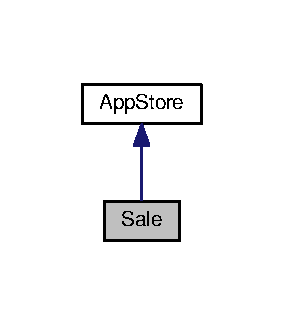
\includegraphics[width=136pt]{class_sale__inherit__graph}
\end{center}
\end{figure}


Collaboration diagram for Sale\-:
\nopagebreak
\begin{figure}[H]
\begin{center}
\leavevmode
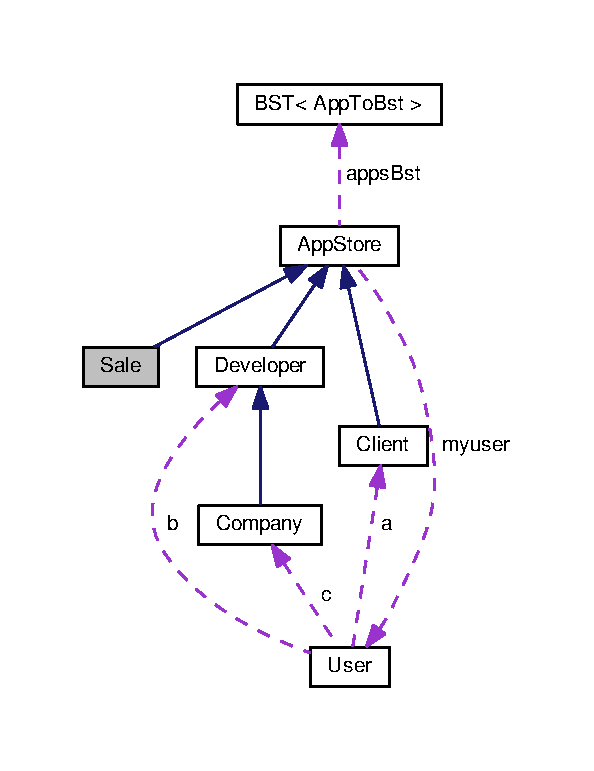
\includegraphics[width=285pt]{class_sale__coll__graph}
\end{center}
\end{figure}
\subsection*{Public Member Functions}
\begin{DoxyCompactItemize}
\item 
\hyperlink{class_sale_a4b941c26295df31d639351b276a11956}{Sale} ()
\begin{DoxyCompactList}\small\item\em Creates an object of type \hyperlink{class_sale}{Sale}. \end{DoxyCompactList}\item 
\hyperlink{class_sale_acb97b345bbd3c7234e84884ac65235e8}{Sale} (\hyperlink{class_app}{App} $\ast$s, \hyperlink{class_client}{Client} $\ast$b)
\begin{DoxyCompactList}\small\item\em Creates an object of type \hyperlink{class_sale}{Sale}. \end{DoxyCompactList}\item 
\hyperlink{struct_date}{Date} \hyperlink{class_sale_a3750d1f83128f3dbe025f2d22f45c19e}{get\-Date} () const 
\begin{DoxyCompactList}\small\item\em gets the date of the sale \end{DoxyCompactList}\item 
void \hyperlink{class_sale_a8b1b584b89a130d854949cc7753ae00f}{set\-Date} (\hyperlink{struct_date}{Date} d)
\begin{DoxyCompactList}\small\item\em sets the date of the sale \end{DoxyCompactList}\item 
int \hyperlink{class_sale_a13124fc8ab466538a0dd3f72f96c466a}{get\-I\-D} () const 
\begin{DoxyCompactList}\small\item\em gets the id of the sale \end{DoxyCompactList}\item 
void \hyperlink{class_sale_abab34b608ead1777ad551932f4f49c7c}{set\-I\-D} (int i)
\begin{DoxyCompactList}\small\item\em sets the id of the sale \end{DoxyCompactList}\item 
int \hyperlink{class_sale_a6c815bb969ece167f3c2b4d3d0dfcd78}{get\-Static\-I\-D} () const 
\begin{DoxyCompactList}\small\item\em gets the static id of the sales \end{DoxyCompactList}\item 
void \hyperlink{class_sale_a5143d0d8e6087109520a535d7a769209}{set\-Static\-I\-D} (int i)
\begin{DoxyCompactList}\small\item\em sets the static id of the sales \end{DoxyCompactList}\item 
\hyperlink{class_app}{App} $\ast$ \hyperlink{class_sale_aefd7c85fd4f0980df644930847550bda}{get\-App\-Sold} () const 
\begin{DoxyCompactList}\small\item\em gets the apps sold \end{DoxyCompactList}\item 
\hyperlink{class_client}{Client} $\ast$ \hyperlink{class_sale_ae1297eab9aa661a5f1b578c7b560faf7}{get\-Buyer} () const 
\begin{DoxyCompactList}\small\item\em gets buyer \end{DoxyCompactList}\item 
void \hyperlink{class_sale_ab058f26afd2ae7f1638f89f8864363bb}{set\-App} (\hyperlink{class_app}{App} $\ast$a)
\begin{DoxyCompactList}\small\item\em sets the app of the sale \end{DoxyCompactList}\item 
void \hyperlink{class_sale_a533bcb3c6d71bb6db576731c5e714b93}{set\-Buyer} (\hyperlink{class_client}{Client} $\ast$b)
\begin{DoxyCompactList}\small\item\em sets the client of the sale \end{DoxyCompactList}\item 
string \hyperlink{class_sale_a8b01a1de2c4c2e5b979eff08db88132a}{get\-User} ()
\begin{DoxyCompactList}\small\item\em gets user \end{DoxyCompactList}\end{DoxyCompactItemize}
\subsection*{Additional Inherited Members}


\subsection{Detailed Description}


Definition at line 1021 of file app\-Store.\-h.



\subsection{Constructor \& Destructor Documentation}
\hypertarget{class_sale_a4b941c26295df31d639351b276a11956}{\index{Sale@{Sale}!Sale@{Sale}}
\index{Sale@{Sale}!Sale@{Sale}}
\subsubsection[{Sale}]{\setlength{\rightskip}{0pt plus 5cm}Sale\-::\-Sale (
\begin{DoxyParamCaption}
{}
\end{DoxyParamCaption}
)}}\label{class_sale_a4b941c26295df31d639351b276a11956}


Creates an object of type \hyperlink{class_sale}{Sale}. 



Definition at line 407 of file app\-Store.\-cpp.

\hypertarget{class_sale_acb97b345bbd3c7234e84884ac65235e8}{\index{Sale@{Sale}!Sale@{Sale}}
\index{Sale@{Sale}!Sale@{Sale}}
\subsubsection[{Sale}]{\setlength{\rightskip}{0pt plus 5cm}Sale\-::\-Sale (
\begin{DoxyParamCaption}
\item[{{\bf App} $\ast$}]{s, }
\item[{{\bf Client} $\ast$}]{b}
\end{DoxyParamCaption}
)}}\label{class_sale_acb97b345bbd3c7234e84884ac65235e8}


Creates an object of type \hyperlink{class_sale}{Sale}. 



Definition at line 421 of file app\-Store.\-cpp.



\subsection{Member Function Documentation}
\hypertarget{class_sale_aefd7c85fd4f0980df644930847550bda}{\index{Sale@{Sale}!get\-App\-Sold@{get\-App\-Sold}}
\index{get\-App\-Sold@{get\-App\-Sold}!Sale@{Sale}}
\subsubsection[{get\-App\-Sold}]{\setlength{\rightskip}{0pt plus 5cm}{\bf App} $\ast$ Sale\-::get\-App\-Sold (
\begin{DoxyParamCaption}
{}
\end{DoxyParamCaption}
) const}}\label{class_sale_aefd7c85fd4f0980df644930847550bda}


gets the apps sold 

\begin{DoxyReturn}{Returns}
the apps sold 
\end{DoxyReturn}


Definition at line 452 of file app\-Store.\-cpp.

\hypertarget{class_sale_ae1297eab9aa661a5f1b578c7b560faf7}{\index{Sale@{Sale}!get\-Buyer@{get\-Buyer}}
\index{get\-Buyer@{get\-Buyer}!Sale@{Sale}}
\subsubsection[{get\-Buyer}]{\setlength{\rightskip}{0pt plus 5cm}{\bf Client} $\ast$ Sale\-::get\-Buyer (
\begin{DoxyParamCaption}
{}
\end{DoxyParamCaption}
) const}}\label{class_sale_ae1297eab9aa661a5f1b578c7b560faf7}


gets buyer 

\begin{DoxyReturn}{Returns}
the $\ast$buyer 
\end{DoxyReturn}


Definition at line 456 of file app\-Store.\-cpp.

\hypertarget{class_sale_a3750d1f83128f3dbe025f2d22f45c19e}{\index{Sale@{Sale}!get\-Date@{get\-Date}}
\index{get\-Date@{get\-Date}!Sale@{Sale}}
\subsubsection[{get\-Date}]{\setlength{\rightskip}{0pt plus 5cm}{\bf Date} Sale\-::get\-Date (
\begin{DoxyParamCaption}
{}
\end{DoxyParamCaption}
) const}}\label{class_sale_a3750d1f83128f3dbe025f2d22f45c19e}


gets the date of the sale 

\begin{DoxyReturn}{Returns}
the date of the sale 
\end{DoxyReturn}


Definition at line 428 of file app\-Store.\-cpp.

\hypertarget{class_sale_a13124fc8ab466538a0dd3f72f96c466a}{\index{Sale@{Sale}!get\-I\-D@{get\-I\-D}}
\index{get\-I\-D@{get\-I\-D}!Sale@{Sale}}
\subsubsection[{get\-I\-D}]{\setlength{\rightskip}{0pt plus 5cm}int Sale\-::get\-I\-D (
\begin{DoxyParamCaption}
{}
\end{DoxyParamCaption}
) const}}\label{class_sale_a13124fc8ab466538a0dd3f72f96c466a}


gets the id of the sale 

\begin{DoxyReturn}{Returns}
the id of the sale 
\end{DoxyReturn}


Definition at line 436 of file app\-Store.\-cpp.

\hypertarget{class_sale_a6c815bb969ece167f3c2b4d3d0dfcd78}{\index{Sale@{Sale}!get\-Static\-I\-D@{get\-Static\-I\-D}}
\index{get\-Static\-I\-D@{get\-Static\-I\-D}!Sale@{Sale}}
\subsubsection[{get\-Static\-I\-D}]{\setlength{\rightskip}{0pt plus 5cm}int Sale\-::get\-Static\-I\-D (
\begin{DoxyParamCaption}
{}
\end{DoxyParamCaption}
) const}}\label{class_sale_a6c815bb969ece167f3c2b4d3d0dfcd78}


gets the static id of the sales 

\begin{DoxyReturn}{Returns}
the static id of the sales 
\end{DoxyReturn}


Definition at line 444 of file app\-Store.\-cpp.

\hypertarget{class_sale_a8b01a1de2c4c2e5b979eff08db88132a}{\index{Sale@{Sale}!get\-User@{get\-User}}
\index{get\-User@{get\-User}!Sale@{Sale}}
\subsubsection[{get\-User}]{\setlength{\rightskip}{0pt plus 5cm}string Sale\-::get\-User (
\begin{DoxyParamCaption}
{}
\end{DoxyParamCaption}
)}}\label{class_sale_a8b01a1de2c4c2e5b979eff08db88132a}


gets user 

\begin{DoxyReturn}{Returns}
the user 
\end{DoxyReturn}


Definition at line 403 of file app\-Store.\-cpp.

\hypertarget{class_sale_ab058f26afd2ae7f1638f89f8864363bb}{\index{Sale@{Sale}!set\-App@{set\-App}}
\index{set\-App@{set\-App}!Sale@{Sale}}
\subsubsection[{set\-App}]{\setlength{\rightskip}{0pt plus 5cm}void Sale\-::set\-App (
\begin{DoxyParamCaption}
\item[{{\bf App} $\ast$}]{a}
\end{DoxyParamCaption}
)}}\label{class_sale_ab058f26afd2ae7f1638f89f8864363bb}


sets the app of the sale 


\begin{DoxyParams}{Parameters}
{\em the} & app of the sale \\
\hline
\end{DoxyParams}


Definition at line 417 of file app\-Store.\-cpp.

\hypertarget{class_sale_a533bcb3c6d71bb6db576731c5e714b93}{\index{Sale@{Sale}!set\-Buyer@{set\-Buyer}}
\index{set\-Buyer@{set\-Buyer}!Sale@{Sale}}
\subsubsection[{set\-Buyer}]{\setlength{\rightskip}{0pt plus 5cm}void Sale\-::set\-Buyer (
\begin{DoxyParamCaption}
\item[{{\bf Client} $\ast$}]{b}
\end{DoxyParamCaption}
)}}\label{class_sale_a533bcb3c6d71bb6db576731c5e714b93}


sets the client of the sale 


\begin{DoxyParams}{Parameters}
{\em the} & buyer of the sale \\
\hline
\end{DoxyParams}


Definition at line 460 of file app\-Store.\-cpp.

\hypertarget{class_sale_a8b1b584b89a130d854949cc7753ae00f}{\index{Sale@{Sale}!set\-Date@{set\-Date}}
\index{set\-Date@{set\-Date}!Sale@{Sale}}
\subsubsection[{set\-Date}]{\setlength{\rightskip}{0pt plus 5cm}void Sale\-::set\-Date (
\begin{DoxyParamCaption}
\item[{{\bf Date}}]{d}
\end{DoxyParamCaption}
)}}\label{class_sale_a8b1b584b89a130d854949cc7753ae00f}


sets the date of the sale 


\begin{DoxyParams}{Parameters}
{\em the} & date of the sale \\
\hline
\end{DoxyParams}


Definition at line 432 of file app\-Store.\-cpp.

\hypertarget{class_sale_abab34b608ead1777ad551932f4f49c7c}{\index{Sale@{Sale}!set\-I\-D@{set\-I\-D}}
\index{set\-I\-D@{set\-I\-D}!Sale@{Sale}}
\subsubsection[{set\-I\-D}]{\setlength{\rightskip}{0pt plus 5cm}void Sale\-::set\-I\-D (
\begin{DoxyParamCaption}
\item[{int}]{i}
\end{DoxyParamCaption}
)}}\label{class_sale_abab34b608ead1777ad551932f4f49c7c}


sets the id of the sale 


\begin{DoxyParams}{Parameters}
{\em the} & id of the sale \\
\hline
\end{DoxyParams}


Definition at line 440 of file app\-Store.\-cpp.

\hypertarget{class_sale_a5143d0d8e6087109520a535d7a769209}{\index{Sale@{Sale}!set\-Static\-I\-D@{set\-Static\-I\-D}}
\index{set\-Static\-I\-D@{set\-Static\-I\-D}!Sale@{Sale}}
\subsubsection[{set\-Static\-I\-D}]{\setlength{\rightskip}{0pt plus 5cm}void Sale\-::set\-Static\-I\-D (
\begin{DoxyParamCaption}
\item[{int}]{i}
\end{DoxyParamCaption}
)}}\label{class_sale_a5143d0d8e6087109520a535d7a769209}


sets the static id of the sales 


\begin{DoxyParams}{Parameters}
{\em the} & static id of the sales \\
\hline
\end{DoxyParams}


Definition at line 448 of file app\-Store.\-cpp.



The documentation for this class was generated from the following files\-:\begin{DoxyCompactItemize}
\item 
src/\hyperlink{app_store_8h}{app\-Store.\-h}\item 
src/\hyperlink{app_store_8cpp}{app\-Store.\-cpp}\end{DoxyCompactItemize}

\hypertarget{class_user}{\section{User Class Reference}
\label{class_user}\index{User@{User}}
}


{\ttfamily \#include $<$app\-Store.\-h$>$}



Collaboration diagram for User\-:
\nopagebreak
\begin{figure}[H]
\begin{center}
\leavevmode
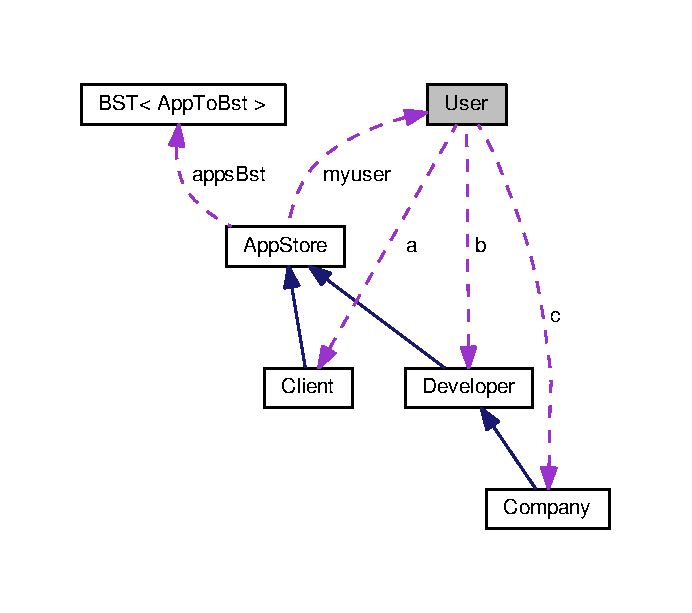
\includegraphics[width=332pt]{class_user__coll__graph}
\end{center}
\end{figure}
\subsection*{Public Member Functions}
\begin{DoxyCompactItemize}
\item 
\hyperlink{class_user_aef527ddb79c49d20a816b6fb47e577e8}{User} (\hyperlink{class_client}{Client} $\ast$\hyperlink{class_user_ac08da4fbb1ade4e24b4a740a0e0e16b3}{a})
\begin{DoxyCompactList}\small\item\em Builds the object. \end{DoxyCompactList}\item 
\hyperlink{class_user_a49e61f50f0af90eb726b48d46d7c95bf}{User} (\hyperlink{class_developer}{Developer} $\ast$\hyperlink{class_user_ac08da4fbb1ade4e24b4a740a0e0e16b3}{a})
\begin{DoxyCompactList}\small\item\em Builds the object. \end{DoxyCompactList}\item 
\hyperlink{class_user_a2d9eef75b371466137c08e6fef58dc18}{User} (\hyperlink{class_company}{Company} $\ast$\hyperlink{class_user_ac08da4fbb1ade4e24b4a740a0e0e16b3}{a})
\begin{DoxyCompactList}\small\item\em Builds the object. \end{DoxyCompactList}\item 
\hyperlink{class_user_a4a0137053e591fbb79d9057dd7d2283d}{User} ()
\begin{DoxyCompactList}\small\item\em Builds the object. \end{DoxyCompactList}\item 
\hyperlink{class_user_ac00b72ad64eb4149f7b21b9f5468c2b2}{$\sim$\-User} ()
\begin{DoxyCompactList}\small\item\em Destroys the object. \end{DoxyCompactList}\end{DoxyCompactItemize}
\subsection*{Public Attributes}
\begin{DoxyCompactItemize}
\item 
\hyperlink{class_client}{Client} $\ast$ \hyperlink{class_user_ac08da4fbb1ade4e24b4a740a0e0e16b3}{a}
\item 
\hyperlink{class_developer}{Developer} $\ast$ \hyperlink{class_user_ac47b21c64dc1d8b02b6ea50a6194dc13}{b}
\item 
\hyperlink{class_company}{Company} $\ast$ \hyperlink{class_user_a98dcb22d99f74e7be130ebfa7ea4ffc1}{c}
\item 
string \hyperlink{class_user_a96c341b10272580def215fcdccfa0d5e}{type}
\end{DoxyCompactItemize}


\subsection{Detailed Description}


Definition at line 65 of file app\-Store.\-h.



\subsection{Constructor \& Destructor Documentation}
\hypertarget{class_user_aef527ddb79c49d20a816b6fb47e577e8}{\index{User@{User}!User@{User}}
\index{User@{User}!User@{User}}
\subsubsection[{User}]{\setlength{\rightskip}{0pt plus 5cm}User\-::\-User (
\begin{DoxyParamCaption}
\item[{{\bf Client} $\ast$}]{a}
\end{DoxyParamCaption}
)}}\label{class_user_aef527ddb79c49d20a816b6fb47e577e8}


Builds the object. 



Definition at line 1638 of file app\-Store.\-cpp.

\hypertarget{class_user_a49e61f50f0af90eb726b48d46d7c95bf}{\index{User@{User}!User@{User}}
\index{User@{User}!User@{User}}
\subsubsection[{User}]{\setlength{\rightskip}{0pt plus 5cm}User\-::\-User (
\begin{DoxyParamCaption}
\item[{{\bf Developer} $\ast$}]{a}
\end{DoxyParamCaption}
)}}\label{class_user_a49e61f50f0af90eb726b48d46d7c95bf}


Builds the object. 



Definition at line 1647 of file app\-Store.\-cpp.

\hypertarget{class_user_a2d9eef75b371466137c08e6fef58dc18}{\index{User@{User}!User@{User}}
\index{User@{User}!User@{User}}
\subsubsection[{User}]{\setlength{\rightskip}{0pt plus 5cm}User\-::\-User (
\begin{DoxyParamCaption}
\item[{{\bf Company} $\ast$}]{a}
\end{DoxyParamCaption}
)}}\label{class_user_a2d9eef75b371466137c08e6fef58dc18}


Builds the object. 



Definition at line 1656 of file app\-Store.\-cpp.

\hypertarget{class_user_a4a0137053e591fbb79d9057dd7d2283d}{\index{User@{User}!User@{User}}
\index{User@{User}!User@{User}}
\subsubsection[{User}]{\setlength{\rightskip}{0pt plus 5cm}User\-::\-User (
\begin{DoxyParamCaption}
{}
\end{DoxyParamCaption}
)}}\label{class_user_a4a0137053e591fbb79d9057dd7d2283d}


Builds the object. 



Definition at line 1665 of file app\-Store.\-cpp.

\hypertarget{class_user_ac00b72ad64eb4149f7b21b9f5468c2b2}{\index{User@{User}!$\sim$\-User@{$\sim$\-User}}
\index{$\sim$\-User@{$\sim$\-User}!User@{User}}
\subsubsection[{$\sim$\-User}]{\setlength{\rightskip}{0pt plus 5cm}User\-::$\sim$\-User (
\begin{DoxyParamCaption}
{}
\end{DoxyParamCaption}
)}}\label{class_user_ac00b72ad64eb4149f7b21b9f5468c2b2}


Destroys the object. 



Definition at line 1675 of file app\-Store.\-cpp.



\subsection{Member Data Documentation}
\hypertarget{class_user_ac08da4fbb1ade4e24b4a740a0e0e16b3}{\index{User@{User}!a@{a}}
\index{a@{a}!User@{User}}
\subsubsection[{a}]{\setlength{\rightskip}{0pt plus 5cm}{\bf Client}$\ast$ User\-::a}}\label{class_user_ac08da4fbb1ade4e24b4a740a0e0e16b3}


Definition at line 67 of file app\-Store.\-h.

\hypertarget{class_user_ac47b21c64dc1d8b02b6ea50a6194dc13}{\index{User@{User}!b@{b}}
\index{b@{b}!User@{User}}
\subsubsection[{b}]{\setlength{\rightskip}{0pt plus 5cm}{\bf Developer}$\ast$ User\-::b}}\label{class_user_ac47b21c64dc1d8b02b6ea50a6194dc13}


Definition at line 68 of file app\-Store.\-h.

\hypertarget{class_user_a98dcb22d99f74e7be130ebfa7ea4ffc1}{\index{User@{User}!c@{c}}
\index{c@{c}!User@{User}}
\subsubsection[{c}]{\setlength{\rightskip}{0pt plus 5cm}{\bf Company}$\ast$ User\-::c}}\label{class_user_a98dcb22d99f74e7be130ebfa7ea4ffc1}


Definition at line 69 of file app\-Store.\-h.

\hypertarget{class_user_a96c341b10272580def215fcdccfa0d5e}{\index{User@{User}!type@{type}}
\index{type@{type}!User@{User}}
\subsubsection[{type}]{\setlength{\rightskip}{0pt plus 5cm}string User\-::type}}\label{class_user_a96c341b10272580def215fcdccfa0d5e}


Definition at line 70 of file app\-Store.\-h.



The documentation for this class was generated from the following files\-:\begin{DoxyCompactItemize}
\item 
src/\hyperlink{app_store_8h}{app\-Store.\-h}\item 
src/\hyperlink{app_store_8cpp}{app\-Store.\-cpp}\end{DoxyCompactItemize}

\chapter{File Documentation}
\hypertarget{aeda_project_8cpp}{\section{src/aeda\-Project.cpp File Reference}
\label{aeda_project_8cpp}\index{src/aeda\-Project.\-cpp@{src/aeda\-Project.\-cpp}}
}
{\ttfamily \#include \char`\"{}menus.\-h\char`\"{}}\\*
Include dependency graph for aeda\-Project.\-cpp\-:
\nopagebreak
\begin{figure}[H]
\begin{center}
\leavevmode
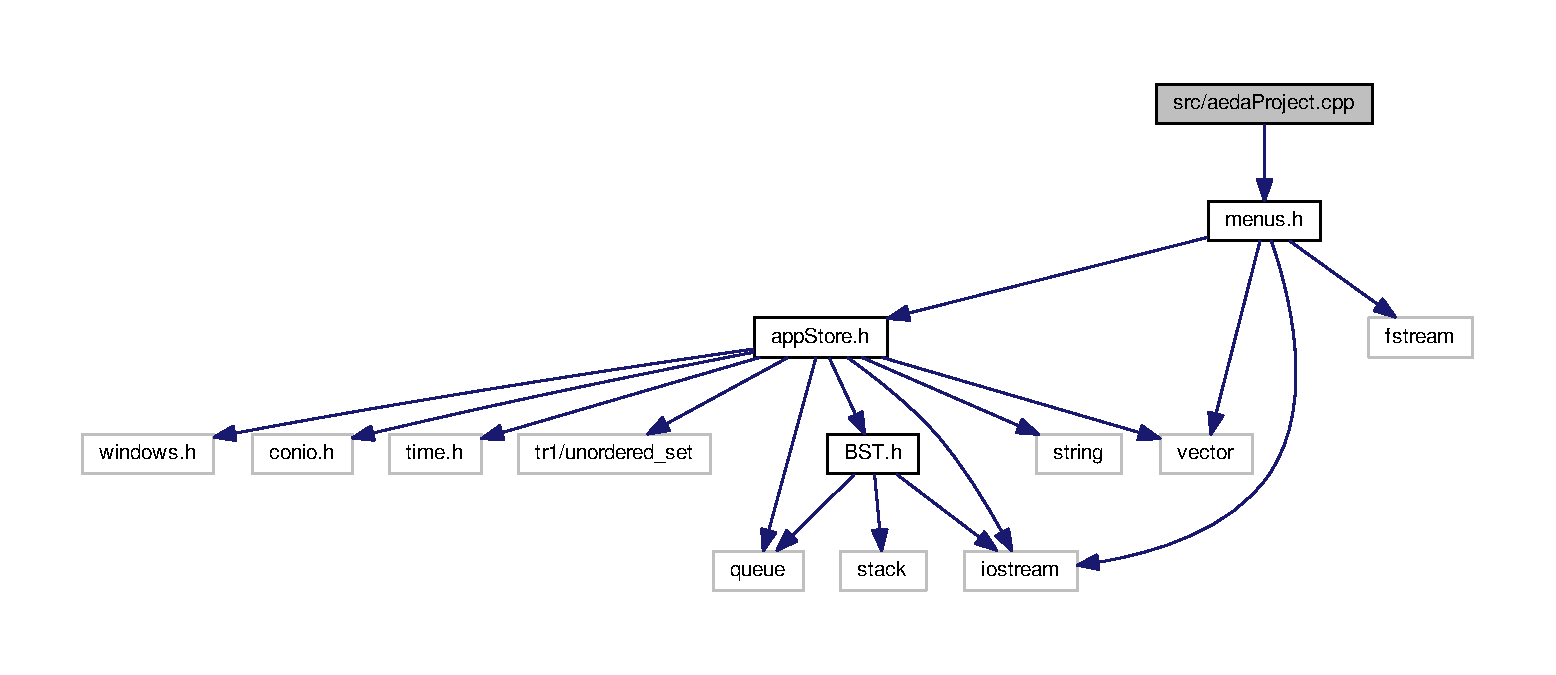
\includegraphics[width=350pt]{aeda_project_8cpp__incl}
\end{center}
\end{figure}
\subsection*{Functions}
\begin{DoxyCompactItemize}
\item 
void \hyperlink{group__aeda_project_ga18a538ccf84de6af3a63e5361de9ab74}{read\-All} (\hyperlink{class_app_store}{App\-Store} \&apps)
\begin{DoxyCompactList}\small\item\em Reads the info from the files in the begining of the program. \end{DoxyCompactList}\item 
void \hyperlink{group__aeda_project_gab8680cb0ec55bb1c599f68575e2804a0}{write\-All} (\hyperlink{class_app_store}{App\-Store} \&apps)
\begin{DoxyCompactList}\small\item\em Wrights the info from the files in the begining of the program. \end{DoxyCompactList}\item 
void \hyperlink{group__aeda_project_ga14cbc22ec0707dc2867f5610ce4914dd}{load\-Hash} (\hyperlink{class_app_store}{App\-Store} \&apps)
\begin{DoxyCompactList}\small\item\em loads the hashtable \end{DoxyCompactList}\item 
int \hyperlink{group__aeda_project_gae66f6b31b5ad750f1fe042a706a4e3d4}{main} ()
\begin{DoxyCompactList}\small\item\em Creates \hyperlink{class_app_store}{App\-Store} and initializes the program. \end{DoxyCompactList}\end{DoxyCompactItemize}

\hypertarget{app_store_8cpp}{\section{src/app\-Store.cpp File Reference}
\label{app_store_8cpp}\index{src/app\-Store.\-cpp@{src/app\-Store.\-cpp}}
}
{\ttfamily \#include \char`\"{}menus.\-h\char`\"{}}\\*
{\ttfamily \#include $<$ctime$>$}\\*
{\ttfamily \#include \char`\"{}B\-S\-T.\-h\char`\"{}}\\*
Include dependency graph for app\-Store.\-cpp\-:
\nopagebreak
\begin{figure}[H]
\begin{center}
\leavevmode
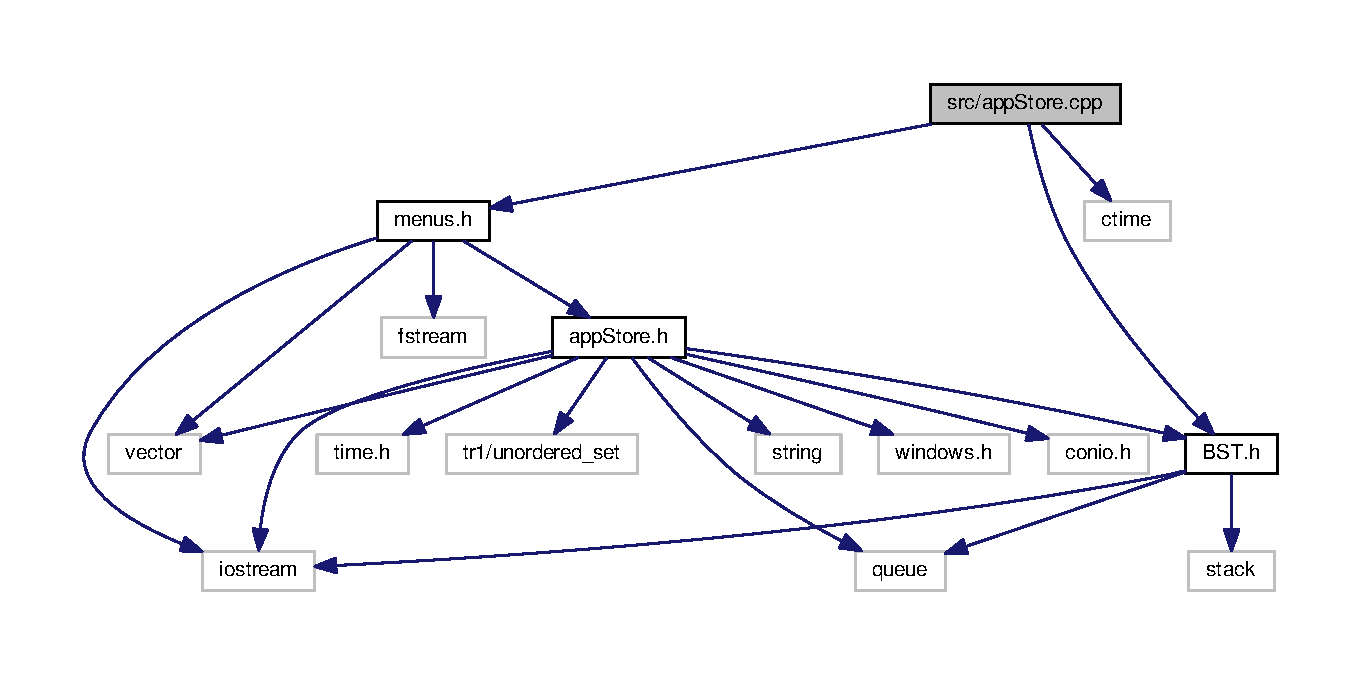
\includegraphics[width=350pt]{app_store_8cpp__incl}
\end{center}
\end{figure}
\subsection*{Functions}
\begin{DoxyCompactItemize}
\item 
void \hyperlink{group__app_store_ga6fba59196281e80b93a79f7941f55cb8}{set\-App\-Id} (int id)
\begin{DoxyCompactList}\small\item\em Changes the global variable to the value given. \end{DoxyCompactList}\item 
void \hyperlink{app_store_8cpp_acc75651fe8b0efccf7399750a63e6259}{set\-Stars} ()
\end{DoxyCompactItemize}
\subsection*{Variables}
\begin{DoxyCompactItemize}
\item 
unsigned int \hyperlink{app_store_8cpp_aef5709c2913265eda10fb983dfd9a1d2}{A\-P\-P\-I\-D} = 0
\item 
unsigned int \hyperlink{app_store_8cpp_a89a3f8c9418ae21771f7074722ca836c}{S\-A\-L\-E\-I\-D} = 0
\item 
\hyperlink{class_app_to_bst}{App\-To\-Bst} \hyperlink{app_store_8cpp_a33e295d1ede1e0f0780ca52b279d2b7a}{initial}
\end{DoxyCompactItemize}


\subsection{Function Documentation}
\hypertarget{app_store_8cpp_acc75651fe8b0efccf7399750a63e6259}{\index{app\-Store.\-cpp@{app\-Store.\-cpp}!set\-Stars@{set\-Stars}}
\index{set\-Stars@{set\-Stars}!appStore.cpp@{app\-Store.\-cpp}}
\subsubsection[{set\-Stars}]{\setlength{\rightskip}{0pt plus 5cm}void set\-Stars (
\begin{DoxyParamCaption}
{}
\end{DoxyParamCaption}
)}}\label{app_store_8cpp_acc75651fe8b0efccf7399750a63e6259}


\subsection{Variable Documentation}
\hypertarget{app_store_8cpp_aef5709c2913265eda10fb983dfd9a1d2}{\index{app\-Store.\-cpp@{app\-Store.\-cpp}!A\-P\-P\-I\-D@{A\-P\-P\-I\-D}}
\index{A\-P\-P\-I\-D@{A\-P\-P\-I\-D}!appStore.cpp@{app\-Store.\-cpp}}
\subsubsection[{A\-P\-P\-I\-D}]{\setlength{\rightskip}{0pt plus 5cm}unsigned int A\-P\-P\-I\-D = 0}}\label{app_store_8cpp_aef5709c2913265eda10fb983dfd9a1d2}


Definition at line 5 of file app\-Store.\-cpp.

\hypertarget{app_store_8cpp_a33e295d1ede1e0f0780ca52b279d2b7a}{\index{app\-Store.\-cpp@{app\-Store.\-cpp}!initial@{initial}}
\index{initial@{initial}!appStore.cpp@{app\-Store.\-cpp}}
\subsubsection[{initial}]{\setlength{\rightskip}{0pt plus 5cm}{\bf App\-To\-Bst} initial}}\label{app_store_8cpp_a33e295d1ede1e0f0780ca52b279d2b7a}


Definition at line 467 of file app\-Store.\-cpp.

\hypertarget{app_store_8cpp_a89a3f8c9418ae21771f7074722ca836c}{\index{app\-Store.\-cpp@{app\-Store.\-cpp}!S\-A\-L\-E\-I\-D@{S\-A\-L\-E\-I\-D}}
\index{S\-A\-L\-E\-I\-D@{S\-A\-L\-E\-I\-D}!appStore.cpp@{app\-Store.\-cpp}}
\subsubsection[{S\-A\-L\-E\-I\-D}]{\setlength{\rightskip}{0pt plus 5cm}unsigned int S\-A\-L\-E\-I\-D = 0}}\label{app_store_8cpp_a89a3f8c9418ae21771f7074722ca836c}


Definition at line 6 of file app\-Store.\-cpp.


\hypertarget{app_store_8h}{\section{src/app\-Store.h File Reference}
\label{app_store_8h}\index{src/app\-Store.\-h@{src/app\-Store.\-h}}
}
{\ttfamily \#include $<$iostream$>$}\\*
{\ttfamily \#include $<$string$>$}\\*
{\ttfamily \#include $<$vector$>$}\\*
{\ttfamily \#include $<$windows.\-h$>$}\\*
{\ttfamily \#include $<$conio.\-h$>$}\\*
{\ttfamily \#include $<$time.\-h$>$}\\*
{\ttfamily \#include $<$tr1/unordered\-\_\-set$>$}\\*
{\ttfamily \#include $<$queue$>$}\\*
{\ttfamily \#include \char`\"{}B\-S\-T.\-h\char`\"{}}\\*
Include dependency graph for app\-Store.\-h\-:
\nopagebreak
\begin{figure}[H]
\begin{center}
\leavevmode
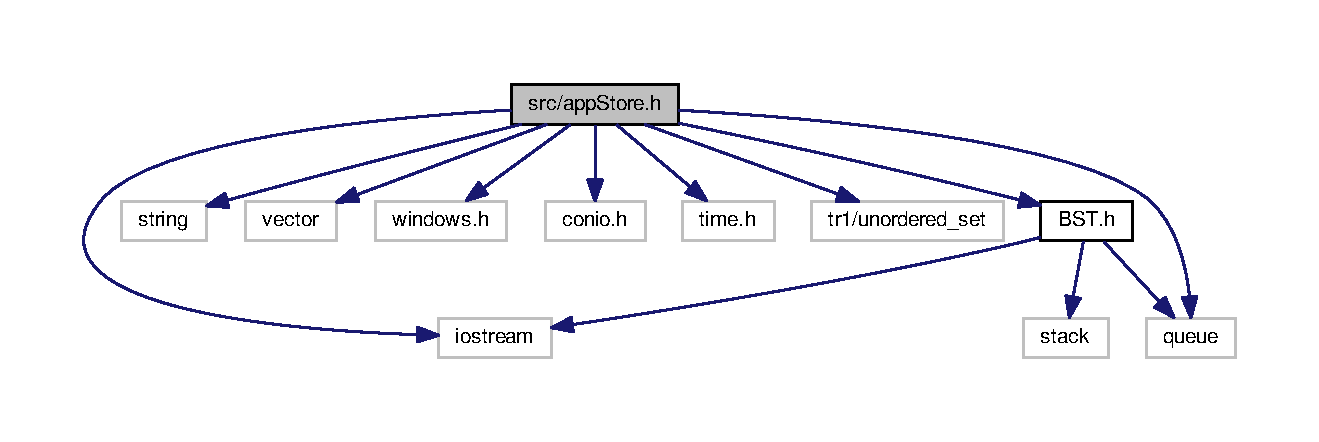
\includegraphics[width=350pt]{app_store_8h__incl}
\end{center}
\end{figure}
This graph shows which files directly or indirectly include this file\-:
\nopagebreak
\begin{figure}[H]
\begin{center}
\leavevmode
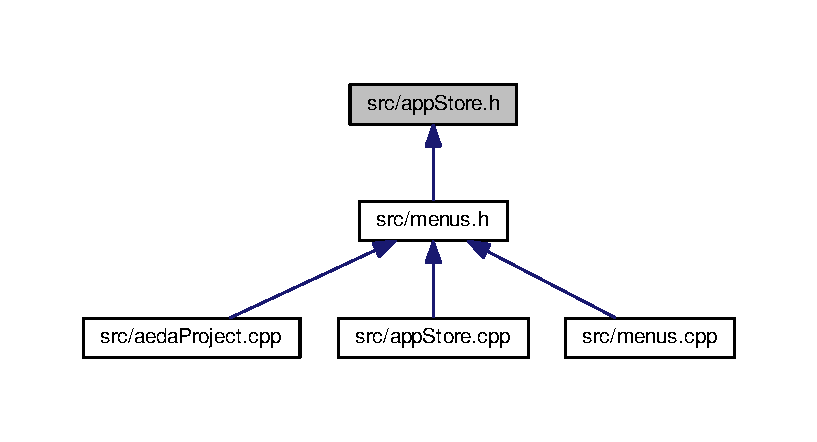
\includegraphics[width=350pt]{app_store_8h__dep__incl}
\end{center}
\end{figure}
\subsection*{Classes}
\begin{DoxyCompactItemize}
\item 
class \hyperlink{class_app_to_bst}{App\-To\-Bst}
\item 
class \hyperlink{class_user}{User}
\item 
class \hyperlink{class_app_store}{App\-Store}
\item 
struct \hyperlink{structclassification}{classification}
\item 
struct \hyperlink{struct_date}{Date}
\item 
class \hyperlink{class_app}{App}
\item 
class \hyperlink{class_app_for_submission}{App\-For\-Submission}
\item 
class \hyperlink{class_client}{Client}
\item 
class \hyperlink{class_developer}{Developer}
\item 
class \hyperlink{class_company}{Company}
\item 
class \hyperlink{class_sale}{Sale}
\item 
class \hyperlink{class_client_not_found}{Client\-Not\-Found}
\item 
class \hyperlink{class_app_not_found}{App\-Not\-Found}
\item 
class \hyperlink{class_out_of_bool_range}{Out\-Of\-Bool\-Range}
\item 
class \hyperlink{class_developer_or_company_not_found}{Developer\-Or\-Company\-Not\-Found}
\item 
class \hyperlink{classfile_not_opened}{file\-Not\-Opened}
\item 
class \hyperlink{class_not_an_app}{Not\-An\-App}
\end{DoxyCompactItemize}
\subsection*{Functions}
\begin{DoxyCompactItemize}
\item 
void \hyperlink{group__app_store_ga6fba59196281e80b93a79f7941f55cb8}{set\-App\-Id} (int id)
\begin{DoxyCompactList}\small\item\em Changes the global variable to the value given. \end{DoxyCompactList}\end{DoxyCompactItemize}

\hypertarget{_b_s_t_8h}{\section{src/\-B\-S\-T.h File Reference}
\label{_b_s_t_8h}\index{src/\-B\-S\-T.\-h@{src/\-B\-S\-T.\-h}}
}
{\ttfamily \#include $<$iostream$>$}\\*
{\ttfamily \#include $<$stack$>$}\\*
{\ttfamily \#include $<$queue$>$}\\*
Include dependency graph for B\-S\-T.\-h\-:
\nopagebreak
\begin{figure}[H]
\begin{center}
\leavevmode
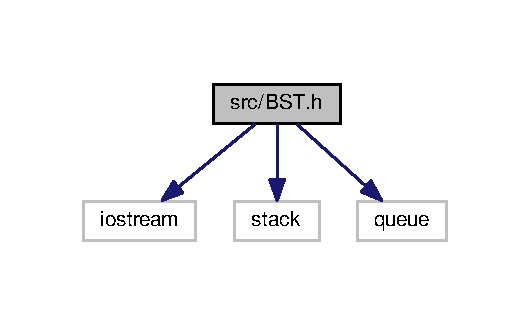
\includegraphics[width=254pt]{_b_s_t_8h__incl}
\end{center}
\end{figure}
This graph shows which files directly or indirectly include this file\-:
\nopagebreak
\begin{figure}[H]
\begin{center}
\leavevmode
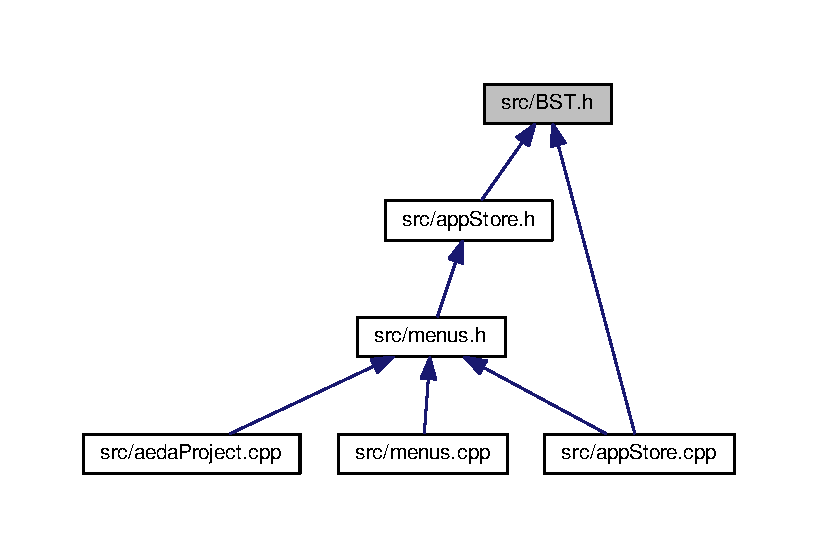
\includegraphics[width=350pt]{_b_s_t_8h__dep__incl}
\end{center}
\end{figure}
\subsection*{Classes}
\begin{DoxyCompactItemize}
\item 
class \hyperlink{class_b_s_t_itr_in}{B\-S\-T\-Itr\-In$<$ Comparable $>$}
\item 
class \hyperlink{class_b_s_t_itr_pre}{B\-S\-T\-Itr\-Pre$<$ Comparable $>$}
\item 
class \hyperlink{class_b_s_t_itr_post}{B\-S\-T\-Itr\-Post$<$ Comparable $>$}
\item 
class \hyperlink{class_b_s_t_itr_level}{B\-S\-T\-Itr\-Level$<$ Comparable $>$}
\item 
class \hyperlink{class_b_s_t}{B\-S\-T$<$ Comparable $>$}
\item 
class \hyperlink{class_binary_node}{Binary\-Node$<$ Comparable $>$}
\item 
class \hyperlink{class_b_s_t}{B\-S\-T$<$ Comparable $>$}
\item 
class \hyperlink{class_b_s_t_itr_post}{B\-S\-T\-Itr\-Post$<$ Comparable $>$}
\item 
class \hyperlink{class_b_s_t_itr_pre}{B\-S\-T\-Itr\-Pre$<$ Comparable $>$}
\item 
class \hyperlink{class_b_s_t_itr_in}{B\-S\-T\-Itr\-In$<$ Comparable $>$}
\item 
class \hyperlink{class_b_s_t_itr_level}{B\-S\-T\-Itr\-Level$<$ Comparable $>$}
\end{DoxyCompactItemize}

\hypertarget{menus_8cpp}{\section{src/menus.cpp File Reference}
\label{menus_8cpp}\index{src/menus.\-cpp@{src/menus.\-cpp}}
}
{\ttfamily \#include \char`\"{}menus.\-h\char`\"{}}\\*
Include dependency graph for menus.\-cpp\-:
\nopagebreak
\begin{figure}[H]
\begin{center}
\leavevmode
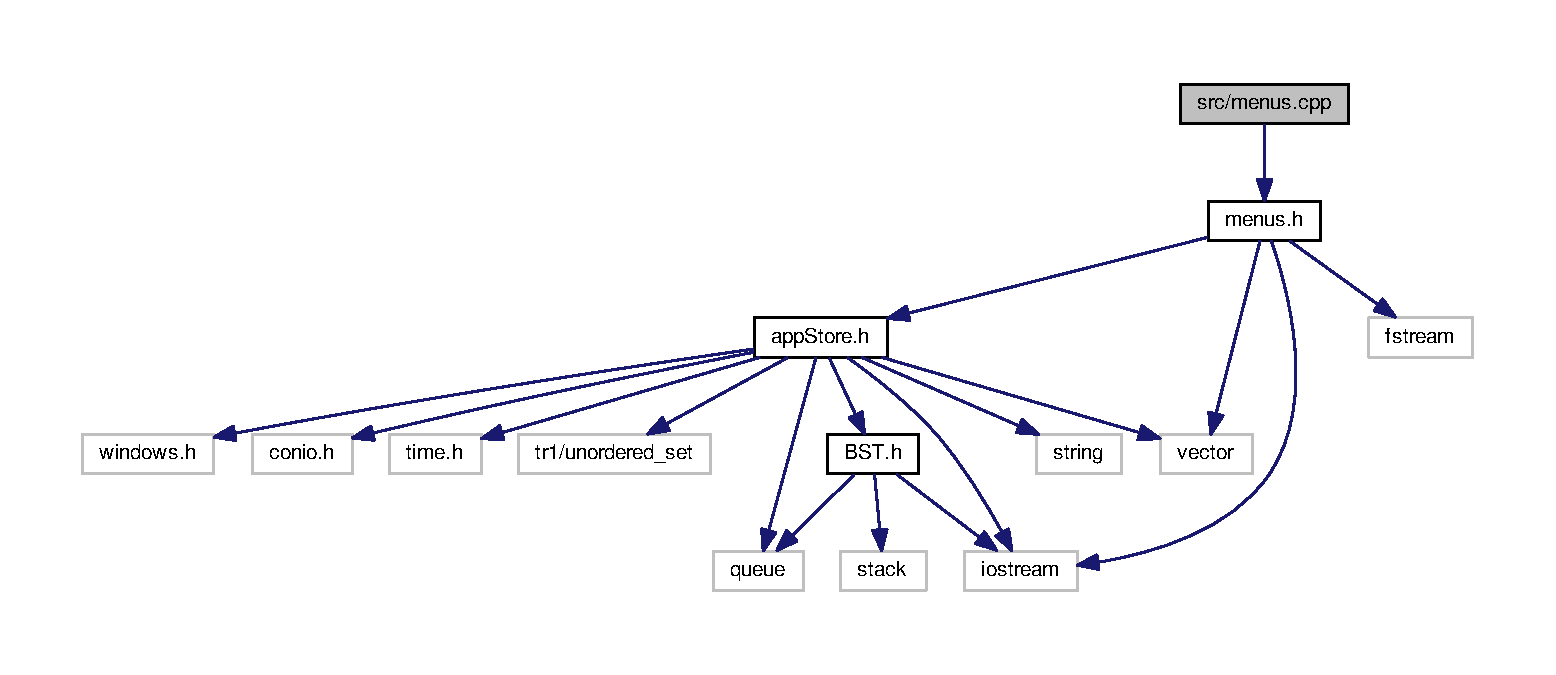
\includegraphics[width=350pt]{menus_8cpp__incl}
\end{center}
\end{figure}
\subsection*{Functions}
{\bf }\par
\begin{DoxyCompactItemize}
\item 
void \hyperlink{menus_8cpp_ac0b822af35be42939c9f4933c3b491bc}{Exit} (void)
\begin{DoxyCompactList}\small\item\em Exit function. \end{DoxyCompactList}\item 
string \hyperlink{menus_8cpp_a7c8229e6d489b26c94512dc5a56510c9}{askpassword} ()
\begin{DoxyCompactList}\small\item\em controls the password access \end{DoxyCompactList}\item 
void \hyperlink{menus_8cpp_aa585ae7d8f5362da92ce8e632e96c1ac}{cs} ()
\begin{DoxyCompactList}\small\item\em clears screen \end{DoxyCompactList}\item 
void \hyperlink{menus_8cpp_a7167f5c196fc5e167bfabde1a730e81d}{pause} ()
\begin{DoxyCompactList}\small\item\em pauses the program \end{DoxyCompactList}\item 
int \hyperlink{menus_8cpp_a00835efb53f4d81f809220267fe4991c}{first\-Screen} ()
\begin{DoxyCompactList}\small\item\em Shows the first screen. \end{DoxyCompactList}\item 
bool \hyperlink{menus_8cpp_a66b2d6899fbd021e387010fec75b91bf}{back} (string a)
\begin{DoxyCompactList}\small\item\em Receives a string and checks if it is equal to $<$-\/. \end{DoxyCompactList}\item 
bool \hyperlink{menus_8cpp_a1ee6cc74c222e723c7fda87574e63f4b}{back} (int a)
\begin{DoxyCompactList}\small\item\em Receives an int and checks if it is equal to $<$-\/. \end{DoxyCompactList}\item 
int \hyperlink{menus_8cpp_a4f88eaae08853208b5bb525d3e03da9d}{sign\-Up\-Menu} (\hyperlink{class_app_store}{App\-Store} \&apps)
\begin{DoxyCompactList}\small\item\em Controls the sign up menu. \end{DoxyCompactList}\item 
int \hyperlink{menus_8cpp_a23a082437ea9566917fc09f1d2ccc7b0}{login\-Menu} (\hyperlink{class_app_store}{App\-Store} \&apps)
\begin{DoxyCompactList}\small\item\em Controls the login menu. \end{DoxyCompactList}\item 
bool \hyperlink{menus_8cpp_a24d0cf281a93649cc324591968b1c64f}{checkusername} (string username, \hyperlink{class_app_store}{App\-Store} \&apps)
\begin{DoxyCompactList}\small\item\em Checks the username. \end{DoxyCompactList}\item 
bool \hyperlink{menus_8cpp_a15ff95b4134182af62dcb4234d47cbe2}{owned} (\hyperlink{class_app}{App} $\ast$myapp, \hyperlink{class_app_store}{App\-Store} $\ast$apps)
\begin{DoxyCompactList}\small\item\em checks if the app is owned \end{DoxyCompactList}\item 
int \hyperlink{menus_8cpp_a17c7e9490a26e40c5d3c6382728b3e36}{check\-User} (string username, string password, \hyperlink{class_app_store}{App\-Store} \&apps)
\begin{DoxyCompactList}\small\item\em Checks user for the right password. \end{DoxyCompactList}\item 
float \hyperlink{menus_8cpp_ab564bbf34f9eacdf62fe5e4bd6fbca9b}{average} (\hyperlink{class_app}{App} $\ast$a, vector$<$ \hyperlink{class_client}{Client} $>$ clients)
\begin{DoxyCompactList}\small\item\em gets the average of an \hyperlink{class_app}{App}'s classification \end{DoxyCompactList}\item 
int \hyperlink{menus_8cpp_a19a2a7e8f371a6a5378668ca4f822960}{app\-Info} (\hyperlink{class_app}{App} $\ast$a, \hyperlink{class_app_store}{App\-Store} \&apps)
\begin{DoxyCompactList}\small\item\em shows somw comments and classifications of the app \end{DoxyCompactList}\item 
int \hyperlink{menus_8cpp_a94b9006ef6c437e3ee9687ac2eeb2f0a}{buy\-Apps} (\hyperlink{class_app_store}{App\-Store} \&apps)
\item 
int \hyperlink{menus_8cpp_ad28464442a48325545db63c47149c9dc}{my\-Apps} (\hyperlink{class_app_store}{App\-Store} \&apps)
\begin{DoxyCompactList}\small\item\em Controls the menu of a clients Inventory. \end{DoxyCompactList}\item 
int \hyperlink{menus_8cpp_acbd29e0ce64bf86be2540f994ccdedf4}{buyall} (\hyperlink{class_app_store}{App\-Store} \&apps)
\begin{DoxyCompactList}\small\item\em Buys all of the items in cart. \end{DoxyCompactList}\item 
int \hyperlink{menus_8cpp_a54946d1d8167333d705a46230f859399}{Client\-Menu} (\hyperlink{class_app_store}{App\-Store} \&apps)
\begin{DoxyCompactList}\small\item\em Controls the Clients Menu. \end{DoxyCompactList}\item 
int \hyperlink{menus_8cpp_ac09423fc4b1ddf2c18f9f9e417092808}{appinfo} (int pos, \hyperlink{class_app_store}{App\-Store} \&apps)
\begin{DoxyCompactList}\small\item\em shows info of an app \end{DoxyCompactList}\item 
int \hyperlink{menus_8cpp_a95e785b125e7e98bc26f847a8533c3d5}{waitingappinfo} (int pos, \hyperlink{class_app_store}{App\-Store} \&apps, \hyperlink{class_app_for_submission}{App\-For\-Submission} a)
\begin{DoxyCompactList}\small\item\em Controls Edition of Apps in queue. \end{DoxyCompactList}\item 
int \hyperlink{menus_8cpp_acd33d00b59cd83fa8ae7f906da6df909}{showapps} (\hyperlink{class_app_store}{App\-Store} \&apps)
\begin{DoxyCompactList}\small\item\em Shows 1 apps info. \end{DoxyCompactList}\item 
int \hyperlink{menus_8cpp_a0e932978a9c7054a1dcc19e706f0ac00}{show\-Apps\-Awating\-Validation} (\hyperlink{class_app_store}{App\-Store} \&apps)
\begin{DoxyCompactList}\small\item\em List Apps Awaiting for Validation on screen. \end{DoxyCompactList}\item 
int \hyperlink{menus_8cpp_a6c744f9403f94a01b85b9e4d77e411d7}{Dev\-Menu} (\hyperlink{class_app_store}{App\-Store} \&apps)
\begin{DoxyCompactList}\small\item\em Dev Menu. \end{DoxyCompactList}\item 
void \hyperlink{menus_8cpp_ace5f8f598c00357636b90d3e674937ec}{Admin\-Client} (\hyperlink{class_app_store}{App\-Store} \&apps)
\begin{DoxyCompactList}\small\item\em C\-R\-U\-D Menu for clients. \end{DoxyCompactList}\item 
void \hyperlink{menus_8cpp_a5a0785ff6e3adff536f33fb89b673290}{Admin\-B\-S\-T} (\hyperlink{class_app_store}{App\-Store} \&apps)
\begin{DoxyCompactList}\small\item\em C\-R\-U\-D Menu for \hyperlink{class_b_s_t}{B\-S\-T}. \end{DoxyCompactList}\item 
void \hyperlink{menus_8cpp_a09fc07852ad9c17d6471e93d07866675}{Admin\-Dev} (\hyperlink{class_app_store}{App\-Store} \&apps)
\begin{DoxyCompactList}\small\item\em C\-R\-U\-D Menu for Devs. \end{DoxyCompactList}\item 
void \hyperlink{menus_8cpp_a648d3f9d841b0b7846a74fff418c11dd}{Admin\-Company} (\hyperlink{class_app_store}{App\-Store} \&apps)
\begin{DoxyCompactList}\small\item\em C\-R\-U\-D Menu for companies. \end{DoxyCompactList}\item 
void \hyperlink{menus_8cpp_a03749b57c45c529b92899e8ef7e7f7d3}{Admin\-Apps} (\hyperlink{class_app_store}{App\-Store} \&apps)
\begin{DoxyCompactList}\small\item\em C\-R\-U\-D Menu for Apps. \end{DoxyCompactList}\item 
void \hyperlink{menus_8cpp_a89dbd52f5f5de893a4ba88975d33b71f}{Admin\-Waiting\-Apps} (\hyperlink{class_app_store}{App\-Store} \&apps)
\begin{DoxyCompactList}\small\item\em C\-R\-U\-D Menu for Apps waiting for validation. \end{DoxyCompactList}\item 
int \hyperlink{menus_8cpp_af1355458d3e1532b79f84ef5e058feaa}{Admin\-Hash\-Apps} (\hyperlink{class_app_store}{App\-Store} \&apps)
\begin{DoxyCompactList}\small\item\em C\-R\-U\-D Menu for Apps out of sales. \end{DoxyCompactList}\item 
int \hyperlink{menus_8cpp_aedbb48a0e8849709ef396ae2e61f3c18}{Admin\-Menu} (\hyperlink{class_app_store}{App\-Store} \&apps)
\begin{DoxyCompactList}\small\item\em C\-R\-U\-D Menus. \end{DoxyCompactList}\item 
int \hyperlink{menus_8cpp_af9720ad08e46ed2f7796588c76d7af21}{Menu} (int a, \hyperlink{class_app_store}{App\-Store} \&apps)
\begin{DoxyCompactList}\small\item\em function to redirect to menu type \end{DoxyCompactList}\item 
\hyperlink{class_app}{App} $\ast$ \hyperlink{menus_8cpp_a3a5f7cc9816336ec914a3f688378ab21}{idtoapp} (int id, \hyperlink{class_app_store}{App\-Store} \&appst)
\begin{DoxyCompactList}\small\item\em Function to get an \hyperlink{class_app}{App} from an I\-D. \end{DoxyCompactList}\item 
vector$<$ \hyperlink{class_client}{Client} $>$ \hyperlink{menus_8cpp_abb046e57ad494277538d50511a16553f}{read\-Clients} (\hyperlink{class_app_store}{App\-Store} \&apps)
\begin{DoxyCompactList}\small\item\em Function to read clients info from text file. \end{DoxyCompactList}\item 
void \hyperlink{menus_8cpp_aced71e1eb6a06c107707665d74d6467f}{write\-Clients} (vector$<$ \hyperlink{class_client}{Client} $>$ vc)
\begin{DoxyCompactList}\small\item\em Function to write clients info to text file. \end{DoxyCompactList}\item 
vector$<$ \hyperlink{class_app}{App} $>$ \hyperlink{menus_8cpp_ab397273ffad40b9e8c08bd27138390e8}{read\-Apps} (\hyperlink{class_app_store}{App\-Store} \&apps)
\begin{DoxyCompactList}\small\item\em Function to read Apps info from text file. \end{DoxyCompactList}\item 
void \hyperlink{menus_8cpp_afcd035b559f35fd9ea1e862a3fd109ea}{read\-Appsto\-Bst} (\hyperlink{class_app_store}{App\-Store} \&apps)
\item 
void \hyperlink{menus_8cpp_ad0841b67a9be8040effd43726dd92267}{write\-Apps\-To\-Bst} (\hyperlink{class_b_s_t}{B\-S\-T}$<$ \hyperlink{class_app_to_bst}{App\-To\-Bst} $>$ app)
\begin{DoxyCompactList}\small\item\em Function to write Apps info to text file. \end{DoxyCompactList}\item 
void \hyperlink{menus_8cpp_a3b6ebfa15859dd53d6926f1886ad5789}{write\-Apps} (vector$<$ \hyperlink{class_app}{App} $>$ \&v)
\item 
vector$<$ \hyperlink{class_developer}{Developer} $>$ \hyperlink{menus_8cpp_af9a05ef922cdb113a8fe7898cf62b8b9}{read\-Devs} (\hyperlink{class_app_store}{App\-Store} \&apps)
\begin{DoxyCompactList}\small\item\em Function to read Devs info from text file. \end{DoxyCompactList}\item 
void \hyperlink{menus_8cpp_aa23062ec4ea8aab93c945f37580c2cbb}{write\-Devs} (\hyperlink{class_app_store}{App\-Store} \&apps)
\begin{DoxyCompactList}\small\item\em Function to write Devs info to text file. \end{DoxyCompactList}\item 
vector$<$ \hyperlink{class_company}{Company} $>$ \hyperlink{menus_8cpp_affb2cadd67c8096436d9a8f06279afe3}{read\-Comp} (\hyperlink{class_app_store}{App\-Store} \&apps)
\begin{DoxyCompactList}\small\item\em Function to read Companies info from text file. \end{DoxyCompactList}\item 
void \hyperlink{menus_8cpp_ac3a783d5fc67b458f098d4866be3160d}{write\-Comp} (vector$<$ \hyperlink{class_company}{Company} $>$ vd)
\begin{DoxyCompactList}\small\item\em Function to write Companies info to text file. \end{DoxyCompactList}\item 
vector$<$ string $>$ \hyperlink{menus_8cpp_a1843c99b6b486725f2f24de1ace88ca0}{read\-Codes} (\hyperlink{class_app_store}{App\-Store} \&apps)
\begin{DoxyCompactList}\small\item\em Function to read Codes from text file. \end{DoxyCompactList}\item 
vector$<$ \hyperlink{class_sale}{Sale} $>$ \hyperlink{menus_8cpp_ae6ced19845f6d11c2269530c97134e6d}{read\-Sales} (\hyperlink{class_app_store}{App\-Store} \&apps)
\begin{DoxyCompactList}\small\item\em Function to read Codes from text file. \end{DoxyCompactList}\item 
void \hyperlink{menus_8cpp_a9d0b2bd4c24cec3b5f6c45068afe44b8}{write\-Sales} (vector$<$ \hyperlink{class_sale}{Sale} $>$ vd)
\begin{DoxyCompactList}\small\item\em Function to write sales to text file. \end{DoxyCompactList}\item 
void \hyperlink{menus_8cpp_a550ef521ba111e4b2bcd7b151b28d991}{top10menu} (\hyperlink{class_app_store}{App\-Store} apps)
\begin{DoxyCompactList}\small\item\em Function to show apps from \hyperlink{class_b_s_t}{B\-S\-T}. \end{DoxyCompactList}\item 
vector$<$ \hyperlink{class_company}{Company} $>$ \hyperlink{menus_8cpp_aea789d7d691da860f926501ae6bc77c1}{read} (\hyperlink{class_app_store}{App\-Store} \&apps)
\begin{DoxyCompactList}\small\item\em Function to read companies info from text file. \end{DoxyCompactList}\item 
void \hyperlink{menus_8cpp_a0dfea7d90f0a83afe03b09acb925ff22}{read\-Vals} (\hyperlink{class_app_store}{App\-Store} \&apps)
\begin{DoxyCompactList}\small\item\em Function read validations from text file. \end{DoxyCompactList}\item 
void \hyperlink{menus_8cpp_a00da6ecf054736e0e2000d32ae1d1d2a}{write\-Vals} (\hyperlink{class_app_store}{App\-Store} \&apps)
\begin{DoxyCompactList}\small\item\em Write Apps waiting for validation info to text file. \end{DoxyCompactList}\end{DoxyCompactItemize}



\subsection{Function Documentation}
\hypertarget{menus_8cpp_a03749b57c45c529b92899e8ef7e7f7d3}{\index{menus.\-cpp@{menus.\-cpp}!Admin\-Apps@{Admin\-Apps}}
\index{Admin\-Apps@{Admin\-Apps}!menus.cpp@{menus.\-cpp}}
\subsubsection[{Admin\-Apps}]{\setlength{\rightskip}{0pt plus 5cm}void Admin\-Apps (
\begin{DoxyParamCaption}
\item[{{\bf App\-Store} \&}]{apps}
\end{DoxyParamCaption}
)}}\label{menus_8cpp_a03749b57c45c529b92899e8ef7e7f7d3}


C\-R\-U\-D Menu for Apps. 


\begin{DoxyParams}{Parameters}
{\em apps} & \hyperlink{class_app_store}{App\-Store} \\
\hline
\end{DoxyParams}


Definition at line 1365 of file menus.\-cpp.

\hypertarget{menus_8cpp_a5a0785ff6e3adff536f33fb89b673290}{\index{menus.\-cpp@{menus.\-cpp}!Admin\-B\-S\-T@{Admin\-B\-S\-T}}
\index{Admin\-B\-S\-T@{Admin\-B\-S\-T}!menus.cpp@{menus.\-cpp}}
\subsubsection[{Admin\-B\-S\-T}]{\setlength{\rightskip}{0pt plus 5cm}void Admin\-B\-S\-T (
\begin{DoxyParamCaption}
\item[{{\bf App\-Store} \&}]{apps}
\end{DoxyParamCaption}
)}}\label{menus_8cpp_a5a0785ff6e3adff536f33fb89b673290}


C\-R\-U\-D Menu for \hyperlink{class_b_s_t}{B\-S\-T}. 


\begin{DoxyParams}{Parameters}
{\em apps} & \hyperlink{class_app_store}{App\-Store} \\
\hline
\end{DoxyParams}


Definition at line 1254 of file menus.\-cpp.

\hypertarget{menus_8cpp_ace5f8f598c00357636b90d3e674937ec}{\index{menus.\-cpp@{menus.\-cpp}!Admin\-Client@{Admin\-Client}}
\index{Admin\-Client@{Admin\-Client}!menus.cpp@{menus.\-cpp}}
\subsubsection[{Admin\-Client}]{\setlength{\rightskip}{0pt plus 5cm}void Admin\-Client (
\begin{DoxyParamCaption}
\item[{{\bf App\-Store} \&}]{apps}
\end{DoxyParamCaption}
)}}\label{menus_8cpp_ace5f8f598c00357636b90d3e674937ec}


C\-R\-U\-D Menu for clients. 


\begin{DoxyParams}{Parameters}
{\em apps} & \hyperlink{class_app_store}{App\-Store} \\
\hline
\end{DoxyParams}


Definition at line 1211 of file menus.\-cpp.

\hypertarget{menus_8cpp_a648d3f9d841b0b7846a74fff418c11dd}{\index{menus.\-cpp@{menus.\-cpp}!Admin\-Company@{Admin\-Company}}
\index{Admin\-Company@{Admin\-Company}!menus.cpp@{menus.\-cpp}}
\subsubsection[{Admin\-Company}]{\setlength{\rightskip}{0pt plus 5cm}void Admin\-Company (
\begin{DoxyParamCaption}
\item[{{\bf App\-Store} \&}]{apps}
\end{DoxyParamCaption}
)}}\label{menus_8cpp_a648d3f9d841b0b7846a74fff418c11dd}


C\-R\-U\-D Menu for companies. 


\begin{DoxyParams}{Parameters}
{\em apps} & \hyperlink{class_app_store}{App\-Store} \\
\hline
\end{DoxyParams}


Definition at line 1329 of file menus.\-cpp.

\hypertarget{menus_8cpp_a09fc07852ad9c17d6471e93d07866675}{\index{menus.\-cpp@{menus.\-cpp}!Admin\-Dev@{Admin\-Dev}}
\index{Admin\-Dev@{Admin\-Dev}!menus.cpp@{menus.\-cpp}}
\subsubsection[{Admin\-Dev}]{\setlength{\rightskip}{0pt plus 5cm}void Admin\-Dev (
\begin{DoxyParamCaption}
\item[{{\bf App\-Store} \&}]{apps}
\end{DoxyParamCaption}
)}}\label{menus_8cpp_a09fc07852ad9c17d6471e93d07866675}


C\-R\-U\-D Menu for Devs. 


\begin{DoxyParams}{Parameters}
{\em apps} & \hyperlink{class_app_store}{App\-Store} \\
\hline
\end{DoxyParams}


Definition at line 1293 of file menus.\-cpp.

\hypertarget{menus_8cpp_af1355458d3e1532b79f84ef5e058feaa}{\index{menus.\-cpp@{menus.\-cpp}!Admin\-Hash\-Apps@{Admin\-Hash\-Apps}}
\index{Admin\-Hash\-Apps@{Admin\-Hash\-Apps}!menus.cpp@{menus.\-cpp}}
\subsubsection[{Admin\-Hash\-Apps}]{\setlength{\rightskip}{0pt plus 5cm}int Admin\-Hash\-Apps (
\begin{DoxyParamCaption}
\item[{{\bf App\-Store} \&}]{apps}
\end{DoxyParamCaption}
)}}\label{menus_8cpp_af1355458d3e1532b79f84ef5e058feaa}


C\-R\-U\-D Menu for Apps out of sales. 


\begin{DoxyParams}{Parameters}
{\em apps} & \hyperlink{class_app_store}{App\-Store} \\
\hline
\end{DoxyParams}


Definition at line 1462 of file menus.\-cpp.

\hypertarget{menus_8cpp_aedbb48a0e8849709ef396ae2e61f3c18}{\index{menus.\-cpp@{menus.\-cpp}!Admin\-Menu@{Admin\-Menu}}
\index{Admin\-Menu@{Admin\-Menu}!menus.cpp@{menus.\-cpp}}
\subsubsection[{Admin\-Menu}]{\setlength{\rightskip}{0pt plus 5cm}int Admin\-Menu (
\begin{DoxyParamCaption}
\item[{{\bf App\-Store} \&}]{apps}
\end{DoxyParamCaption}
)}}\label{menus_8cpp_aedbb48a0e8849709ef396ae2e61f3c18}


C\-R\-U\-D Menus. 


\begin{DoxyParams}{Parameters}
{\em apps} & \hyperlink{class_app_store}{App\-Store} \\
\hline
\end{DoxyParams}


Definition at line 1498 of file menus.\-cpp.

\hypertarget{menus_8cpp_a89dbd52f5f5de893a4ba88975d33b71f}{\index{menus.\-cpp@{menus.\-cpp}!Admin\-Waiting\-Apps@{Admin\-Waiting\-Apps}}
\index{Admin\-Waiting\-Apps@{Admin\-Waiting\-Apps}!menus.cpp@{menus.\-cpp}}
\subsubsection[{Admin\-Waiting\-Apps}]{\setlength{\rightskip}{0pt plus 5cm}void Admin\-Waiting\-Apps (
\begin{DoxyParamCaption}
\item[{{\bf App\-Store} \&}]{apps}
\end{DoxyParamCaption}
)}}\label{menus_8cpp_a89dbd52f5f5de893a4ba88975d33b71f}


C\-R\-U\-D Menu for Apps waiting for validation. 


\begin{DoxyParams}{Parameters}
{\em apps} & \hyperlink{class_app_store}{App\-Store} \\
\hline
\end{DoxyParams}


Definition at line 1419 of file menus.\-cpp.

\hypertarget{menus_8cpp_a19a2a7e8f371a6a5378668ca4f822960}{\index{menus.\-cpp@{menus.\-cpp}!app\-Info@{app\-Info}}
\index{app\-Info@{app\-Info}!menus.cpp@{menus.\-cpp}}
\subsubsection[{app\-Info}]{\setlength{\rightskip}{0pt plus 5cm}int app\-Info (
\begin{DoxyParamCaption}
\item[{{\bf App} $\ast$}]{a, }
\item[{{\bf App\-Store} \&}]{apps}
\end{DoxyParamCaption}
)}}\label{menus_8cpp_a19a2a7e8f371a6a5378668ca4f822960}


shows somw comments and classifications of the app 


\begin{DoxyParams}{Parameters}
{\em $\ast$a} & \hyperlink{class_app}{App} \\
\hline
{\em apps} & \hyperlink{class_app_store}{App\-Store}\\
\hline
\end{DoxyParams}
\begin{DoxyReturn}{Returns}
Returns 0 
\end{DoxyReturn}


Definition at line 362 of file menus.\-cpp.

\hypertarget{menus_8cpp_ac09423fc4b1ddf2c18f9f9e417092808}{\index{menus.\-cpp@{menus.\-cpp}!appinfo@{appinfo}}
\index{appinfo@{appinfo}!menus.cpp@{menus.\-cpp}}
\subsubsection[{appinfo}]{\setlength{\rightskip}{0pt plus 5cm}int appinfo (
\begin{DoxyParamCaption}
\item[{int}]{pos, }
\item[{{\bf App\-Store} \&}]{apps}
\end{DoxyParamCaption}
)}}\label{menus_8cpp_ac09423fc4b1ddf2c18f9f9e417092808}


shows info of an app 


\begin{DoxyParams}{Parameters}
{\em pos} & position \\
\hline
{\em apps} & \hyperlink{class_app_store}{App\-Store}\\
\hline
\end{DoxyParams}
\begin{DoxyReturn}{Returns}
returns 0 
\end{DoxyReturn}


Definition at line 771 of file menus.\-cpp.

\hypertarget{menus_8cpp_a7c8229e6d489b26c94512dc5a56510c9}{\index{menus.\-cpp@{menus.\-cpp}!askpassword@{askpassword}}
\index{askpassword@{askpassword}!menus.cpp@{menus.\-cpp}}
\subsubsection[{askpassword}]{\setlength{\rightskip}{0pt plus 5cm}string askpassword (
\begin{DoxyParamCaption}
{}
\end{DoxyParamCaption}
)}}\label{menus_8cpp_a7c8229e6d489b26c94512dc5a56510c9}


controls the password access 

\begin{DoxyReturn}{Returns}
password 
\end{DoxyReturn}


Definition at line 22 of file menus.\-cpp.

\hypertarget{menus_8cpp_ab564bbf34f9eacdf62fe5e4bd6fbca9b}{\index{menus.\-cpp@{menus.\-cpp}!average@{average}}
\index{average@{average}!menus.cpp@{menus.\-cpp}}
\subsubsection[{average}]{\setlength{\rightskip}{0pt plus 5cm}float average (
\begin{DoxyParamCaption}
\item[{{\bf App} $\ast$}]{a, }
\item[{vector$<$ {\bf Client} $>$}]{clients}
\end{DoxyParamCaption}
)}}\label{menus_8cpp_ab564bbf34f9eacdf62fe5e4bd6fbca9b}


gets the average of an \hyperlink{class_app}{App}'s classification 


\begin{DoxyParams}{Parameters}
{\em $\ast$a} & \hyperlink{class_app}{App} \\
\hline
{\em clients} & vector of the clients\\
\hline
\end{DoxyParams}
\begin{DoxyReturn}{Returns}
returns the average classification 
\end{DoxyReturn}


Definition at line 329 of file menus.\-cpp.

\hypertarget{menus_8cpp_a66b2d6899fbd021e387010fec75b91bf}{\index{menus.\-cpp@{menus.\-cpp}!back@{back}}
\index{back@{back}!menus.cpp@{menus.\-cpp}}
\subsubsection[{back}]{\setlength{\rightskip}{0pt plus 5cm}bool back (
\begin{DoxyParamCaption}
\item[{string}]{a}
\end{DoxyParamCaption}
)}}\label{menus_8cpp_a66b2d6899fbd021e387010fec75b91bf}


Receives a string and checks if it is equal to $<$-\/. 


\begin{DoxyParams}{Parameters}
{\em a} & string to check\\
\hline
\end{DoxyParams}
\begin{DoxyReturn}{Returns}
Returns true if equal and false otherwise 
\end{DoxyReturn}


Definition at line 91 of file menus.\-cpp.

\hypertarget{menus_8cpp_a1ee6cc74c222e723c7fda87574e63f4b}{\index{menus.\-cpp@{menus.\-cpp}!back@{back}}
\index{back@{back}!menus.cpp@{menus.\-cpp}}
\subsubsection[{back}]{\setlength{\rightskip}{0pt plus 5cm}bool back (
\begin{DoxyParamCaption}
\item[{int}]{a}
\end{DoxyParamCaption}
)}}\label{menus_8cpp_a1ee6cc74c222e723c7fda87574e63f4b}


Receives an int and checks if it is equal to $<$-\/. 


\begin{DoxyParams}{Parameters}
{\em a} & int to check\\
\hline
\end{DoxyParams}
\begin{DoxyReturn}{Returns}
Returns true if equal and false otherwise 
\end{DoxyReturn}


Definition at line 108 of file menus.\-cpp.

\hypertarget{menus_8cpp_acbd29e0ce64bf86be2540f994ccdedf4}{\index{menus.\-cpp@{menus.\-cpp}!buyall@{buyall}}
\index{buyall@{buyall}!menus.cpp@{menus.\-cpp}}
\subsubsection[{buyall}]{\setlength{\rightskip}{0pt plus 5cm}int buyall (
\begin{DoxyParamCaption}
\item[{{\bf App\-Store} \&}]{apps}
\end{DoxyParamCaption}
)}}\label{menus_8cpp_acbd29e0ce64bf86be2540f994ccdedf4}


Buys all of the items in cart. 


\begin{DoxyParams}{Parameters}
{\em \hyperlink{class_app_store}{App\-Store}} & \\
\hline
\end{DoxyParams}
\begin{DoxyReturn}{Returns}
Returns 
\end{DoxyReturn}


Definition at line 553 of file menus.\-cpp.

\hypertarget{menus_8cpp_a94b9006ef6c437e3ee9687ac2eeb2f0a}{\index{menus.\-cpp@{menus.\-cpp}!buy\-Apps@{buy\-Apps}}
\index{buy\-Apps@{buy\-Apps}!menus.cpp@{menus.\-cpp}}
\subsubsection[{buy\-Apps}]{\setlength{\rightskip}{0pt plus 5cm}int buy\-Apps (
\begin{DoxyParamCaption}
\item[{{\bf App\-Store} \&}]{apps}
\end{DoxyParamCaption}
)}}\label{menus_8cpp_a94b9006ef6c437e3ee9687ac2eeb2f0a}
shows and controls the menu of the clients purchase


\begin{DoxyParams}{Parameters}
{\em apps} & \hyperlink{class_app_store}{App\-Store}\\
\hline
\end{DoxyParams}
\begin{DoxyReturn}{Returns}
Returns 1 
\end{DoxyReturn}


Definition at line 451 of file menus.\-cpp.

\hypertarget{menus_8cpp_a17c7e9490a26e40c5d3c6382728b3e36}{\index{menus.\-cpp@{menus.\-cpp}!check\-User@{check\-User}}
\index{check\-User@{check\-User}!menus.cpp@{menus.\-cpp}}
\subsubsection[{check\-User}]{\setlength{\rightskip}{0pt plus 5cm}int check\-User (
\begin{DoxyParamCaption}
\item[{string}]{username, }
\item[{string}]{password, }
\item[{{\bf App\-Store} \&}]{apps}
\end{DoxyParamCaption}
)}}\label{menus_8cpp_a17c7e9490a26e40c5d3c6382728b3e36}


Checks user for the right password. 


\begin{DoxyParams}{Parameters}
{\em username} & name of the user \\
\hline
{\em password} & password of theuser \\
\hline
{\em apps} & Apps\\
\hline
\end{DoxyParams}
\begin{DoxyReturn}{Returns}
returns 0-\/2 
\end{DoxyReturn}


Definition at line 292 of file menus.\-cpp.

\hypertarget{menus_8cpp_a24d0cf281a93649cc324591968b1c64f}{\index{menus.\-cpp@{menus.\-cpp}!checkusername@{checkusername}}
\index{checkusername@{checkusername}!menus.cpp@{menus.\-cpp}}
\subsubsection[{checkusername}]{\setlength{\rightskip}{0pt plus 5cm}bool checkusername (
\begin{DoxyParamCaption}
\item[{string}]{username, }
\item[{{\bf App\-Store} \&}]{apps}
\end{DoxyParamCaption}
)}}\label{menus_8cpp_a24d0cf281a93649cc324591968b1c64f}


Checks the username. 


\begin{DoxyParams}{Parameters}
{\em username} & the username to check \\
\hline
{\em apps} & with the info\\
\hline
\end{DoxyParams}
\begin{DoxyReturn}{Returns}
returns true/false depending on que check of the username 
\end{DoxyReturn}


Definition at line 244 of file menus.\-cpp.

\hypertarget{menus_8cpp_a54946d1d8167333d705a46230f859399}{\index{menus.\-cpp@{menus.\-cpp}!Client\-Menu@{Client\-Menu}}
\index{Client\-Menu@{Client\-Menu}!menus.cpp@{menus.\-cpp}}
\subsubsection[{Client\-Menu}]{\setlength{\rightskip}{0pt plus 5cm}int Client\-Menu (
\begin{DoxyParamCaption}
\item[{{\bf App\-Store} \&}]{apps}
\end{DoxyParamCaption}
)}}\label{menus_8cpp_a54946d1d8167333d705a46230f859399}


Controls the Clients Menu. 


\begin{DoxyParams}{Parameters}
{\em apps} & \hyperlink{class_app_store}{App\-Store}\\
\hline
\end{DoxyParams}
\begin{DoxyReturn}{Returns}
returns 0 
\end{DoxyReturn}


Definition at line 660 of file menus.\-cpp.

\hypertarget{menus_8cpp_aa585ae7d8f5362da92ce8e632e96c1ac}{\index{menus.\-cpp@{menus.\-cpp}!cs@{cs}}
\index{cs@{cs}!menus.cpp@{menus.\-cpp}}
\subsubsection[{cs}]{\setlength{\rightskip}{0pt plus 5cm}void cs (
\begin{DoxyParamCaption}
{}
\end{DoxyParamCaption}
)}}\label{menus_8cpp_aa585ae7d8f5362da92ce8e632e96c1ac}


clears screen 



Definition at line 62 of file menus.\-cpp.

\hypertarget{menus_8cpp_a6c744f9403f94a01b85b9e4d77e411d7}{\index{menus.\-cpp@{menus.\-cpp}!Dev\-Menu@{Dev\-Menu}}
\index{Dev\-Menu@{Dev\-Menu}!menus.cpp@{menus.\-cpp}}
\subsubsection[{Dev\-Menu}]{\setlength{\rightskip}{0pt plus 5cm}int Dev\-Menu (
\begin{DoxyParamCaption}
\item[{{\bf App\-Store} \&}]{apps}
\end{DoxyParamCaption}
)}}\label{menus_8cpp_a6c744f9403f94a01b85b9e4d77e411d7}


Dev Menu. 


\begin{DoxyParams}{Parameters}
{\em apps} & \hyperlink{class_app_store}{App\-Store} \\
\hline
\end{DoxyParams}


Definition at line 1072 of file menus.\-cpp.

\hypertarget{menus_8cpp_ac0b822af35be42939c9f4933c3b491bc}{\index{menus.\-cpp@{menus.\-cpp}!Exit@{Exit}}
\index{Exit@{Exit}!menus.cpp@{menus.\-cpp}}
\subsubsection[{Exit}]{\setlength{\rightskip}{0pt plus 5cm}void Exit (
\begin{DoxyParamCaption}
\item[{void}]{}
\end{DoxyParamCaption}
)}}\label{menus_8cpp_ac0b822af35be42939c9f4933c3b491bc}


Exit function. 

defgroup Menus Menus

Controls the menus and the interface 

Definition at line 11 of file menus.\-cpp.

\hypertarget{menus_8cpp_a00835efb53f4d81f809220267fe4991c}{\index{menus.\-cpp@{menus.\-cpp}!first\-Screen@{first\-Screen}}
\index{first\-Screen@{first\-Screen}!menus.cpp@{menus.\-cpp}}
\subsubsection[{first\-Screen}]{\setlength{\rightskip}{0pt plus 5cm}int first\-Screen (
\begin{DoxyParamCaption}
{}
\end{DoxyParamCaption}
)}}\label{menus_8cpp_a00835efb53f4d81f809220267fe4991c}


Shows the first screen. 



Definition at line 75 of file menus.\-cpp.

\hypertarget{menus_8cpp_a3a5f7cc9816336ec914a3f688378ab21}{\index{menus.\-cpp@{menus.\-cpp}!idtoapp@{idtoapp}}
\index{idtoapp@{idtoapp}!menus.cpp@{menus.\-cpp}}
\subsubsection[{idtoapp}]{\setlength{\rightskip}{0pt plus 5cm}{\bf App}$\ast$ idtoapp (
\begin{DoxyParamCaption}
\item[{int}]{id, }
\item[{{\bf App\-Store} \&}]{appst}
\end{DoxyParamCaption}
)}}\label{menus_8cpp_a3a5f7cc9816336ec914a3f688378ab21}


Function to get an \hyperlink{class_app}{App} from an I\-D. 


\begin{DoxyParams}{Parameters}
{\em apps} & \hyperlink{class_app_store}{App\-Store} \\
\hline
\end{DoxyParams}
\begin{DoxyReturn}{Returns}
Returns an app Pointer with that I\-D 
\end{DoxyReturn}


Definition at line 1573 of file menus.\-cpp.

\hypertarget{menus_8cpp_a23a082437ea9566917fc09f1d2ccc7b0}{\index{menus.\-cpp@{menus.\-cpp}!login\-Menu@{login\-Menu}}
\index{login\-Menu@{login\-Menu}!menus.cpp@{menus.\-cpp}}
\subsubsection[{login\-Menu}]{\setlength{\rightskip}{0pt plus 5cm}int login\-Menu (
\begin{DoxyParamCaption}
\item[{{\bf App\-Store} \&}]{apps}
\end{DoxyParamCaption}
)}}\label{menus_8cpp_a23a082437ea9566917fc09f1d2ccc7b0}


Controls the login menu. 


\begin{DoxyParams}{Parameters}
{\em apps} & \hyperlink{class_app_store}{App\-Store}\\
\hline
\end{DoxyParams}
\begin{DoxyReturn}{Returns}
returns 0 
\end{DoxyReturn}


Definition at line 209 of file menus.\-cpp.

\hypertarget{menus_8cpp_af9720ad08e46ed2f7796588c76d7af21}{\index{menus.\-cpp@{menus.\-cpp}!Menu@{Menu}}
\index{Menu@{Menu}!menus.cpp@{menus.\-cpp}}
\subsubsection[{Menu}]{\setlength{\rightskip}{0pt plus 5cm}int Menu (
\begin{DoxyParamCaption}
\item[{int}]{a, }
\item[{{\bf App\-Store} \&}]{apps}
\end{DoxyParamCaption}
)}}\label{menus_8cpp_af9720ad08e46ed2f7796588c76d7af21}


function to redirect to menu type 


\begin{DoxyParams}{Parameters}
{\em apps} & \hyperlink{class_app_store}{App\-Store} \\
\hline
{\em a} & type of menun (from 1 to 3) \\
\hline
\end{DoxyParams}


Definition at line 1543 of file menus.\-cpp.

\hypertarget{menus_8cpp_ad28464442a48325545db63c47149c9dc}{\index{menus.\-cpp@{menus.\-cpp}!my\-Apps@{my\-Apps}}
\index{my\-Apps@{my\-Apps}!menus.cpp@{menus.\-cpp}}
\subsubsection[{my\-Apps}]{\setlength{\rightskip}{0pt plus 5cm}int my\-Apps (
\begin{DoxyParamCaption}
\item[{{\bf App\-Store} \&}]{apps}
\end{DoxyParamCaption}
)}}\label{menus_8cpp_ad28464442a48325545db63c47149c9dc}


Controls the menu of a clients Inventory. 


\begin{DoxyParams}{Parameters}
{\em apps} & \hyperlink{class_app_store}{App\-Store}\\
\hline
\end{DoxyParams}
\begin{DoxyReturn}{Returns}
Returns 
\end{DoxyReturn}


Definition at line 491 of file menus.\-cpp.

\hypertarget{menus_8cpp_a15ff95b4134182af62dcb4234d47cbe2}{\index{menus.\-cpp@{menus.\-cpp}!owned@{owned}}
\index{owned@{owned}!menus.cpp@{menus.\-cpp}}
\subsubsection[{owned}]{\setlength{\rightskip}{0pt plus 5cm}bool owned (
\begin{DoxyParamCaption}
\item[{{\bf App} $\ast$}]{myapp, }
\item[{{\bf App\-Store} $\ast$}]{apps}
\end{DoxyParamCaption}
)}}\label{menus_8cpp_a15ff95b4134182af62dcb4234d47cbe2}


checks if the app is owned 


\begin{DoxyParams}{Parameters}
{\em App$\ast$} & myapp \\
\hline
{\em apps} & \hyperlink{class_app_store}{App\-Store}\\
\hline
\end{DoxyParams}
\begin{DoxyReturn}{Returns}
Returns true or false depending on if it is owned 
\end{DoxyReturn}


Definition at line 273 of file menus.\-cpp.

\hypertarget{menus_8cpp_a7167f5c196fc5e167bfabde1a730e81d}{\index{menus.\-cpp@{menus.\-cpp}!pause@{pause}}
\index{pause@{pause}!menus.cpp@{menus.\-cpp}}
\subsubsection[{pause}]{\setlength{\rightskip}{0pt plus 5cm}void pause (
\begin{DoxyParamCaption}
{}
\end{DoxyParamCaption}
)}}\label{menus_8cpp_a7167f5c196fc5e167bfabde1a730e81d}


pauses the program 



Definition at line 67 of file menus.\-cpp.

\hypertarget{menus_8cpp_aea789d7d691da860f926501ae6bc77c1}{\index{menus.\-cpp@{menus.\-cpp}!read@{read}}
\index{read@{read}!menus.cpp@{menus.\-cpp}}
\subsubsection[{read}]{\setlength{\rightskip}{0pt plus 5cm}vector$<${\bf Company}$>$ read (
\begin{DoxyParamCaption}
\item[{{\bf App\-Store} \&}]{apps}
\end{DoxyParamCaption}
)}}\label{menus_8cpp_aea789d7d691da860f926501ae6bc77c1}


Function to read companies info from text file. 


\begin{DoxyParams}{Parameters}
{\em apps} & \hyperlink{class_app_store}{App\-Store} data structure \\
\hline
\end{DoxyParams}
\begin{DoxyReturn}{Returns}
vector of companies 
\end{DoxyReturn}


Definition at line 2105 of file menus.\-cpp.

\hypertarget{menus_8cpp_ab397273ffad40b9e8c08bd27138390e8}{\index{menus.\-cpp@{menus.\-cpp}!read\-Apps@{read\-Apps}}
\index{read\-Apps@{read\-Apps}!menus.cpp@{menus.\-cpp}}
\subsubsection[{read\-Apps}]{\setlength{\rightskip}{0pt plus 5cm}vector$<${\bf App}$>$ read\-Apps (
\begin{DoxyParamCaption}
\item[{{\bf App\-Store} \&}]{apps}
\end{DoxyParamCaption}
)}}\label{menus_8cpp_ab397273ffad40b9e8c08bd27138390e8}


Function to read Apps info from text file. 


\begin{DoxyParams}{Parameters}
{\em apps} & \hyperlink{class_app_store}{App\-Store} \\
\hline
\end{DoxyParams}
\begin{DoxyReturn}{Returns}
vector of apps 
\end{DoxyReturn}


Definition at line 1685 of file menus.\-cpp.

\hypertarget{menus_8cpp_afcd035b559f35fd9ea1e862a3fd109ea}{\index{menus.\-cpp@{menus.\-cpp}!read\-Appsto\-Bst@{read\-Appsto\-Bst}}
\index{read\-Appsto\-Bst@{read\-Appsto\-Bst}!menus.cpp@{menus.\-cpp}}
\subsubsection[{read\-Appsto\-Bst}]{\setlength{\rightskip}{0pt plus 5cm}void read\-Appsto\-Bst (
\begin{DoxyParamCaption}
\item[{{\bf App\-Store} \&}]{apps}
\end{DoxyParamCaption}
)}}\label{menus_8cpp_afcd035b559f35fd9ea1e862a3fd109ea}


Definition at line 1720 of file menus.\-cpp.

\hypertarget{menus_8cpp_abb046e57ad494277538d50511a16553f}{\index{menus.\-cpp@{menus.\-cpp}!read\-Clients@{read\-Clients}}
\index{read\-Clients@{read\-Clients}!menus.cpp@{menus.\-cpp}}
\subsubsection[{read\-Clients}]{\setlength{\rightskip}{0pt plus 5cm}vector$<${\bf Client}$>$ read\-Clients (
\begin{DoxyParamCaption}
\item[{{\bf App\-Store} \&}]{apps}
\end{DoxyParamCaption}
)}}\label{menus_8cpp_abb046e57ad494277538d50511a16553f}


Function to read clients info from text file. 


\begin{DoxyParams}{Parameters}
{\em apps} & \hyperlink{class_app_store}{App\-Store} \\
\hline
\end{DoxyParams}


Definition at line 1590 of file menus.\-cpp.

\hypertarget{menus_8cpp_a1843c99b6b486725f2f24de1ace88ca0}{\index{menus.\-cpp@{menus.\-cpp}!read\-Codes@{read\-Codes}}
\index{read\-Codes@{read\-Codes}!menus.cpp@{menus.\-cpp}}
\subsubsection[{read\-Codes}]{\setlength{\rightskip}{0pt plus 5cm}vector$<$string$>$ read\-Codes (
\begin{DoxyParamCaption}
\item[{{\bf App\-Store} \&}]{apps}
\end{DoxyParamCaption}
)}}\label{menus_8cpp_a1843c99b6b486725f2f24de1ace88ca0}


Function to read Codes from text file. 


\begin{DoxyParams}{Parameters}
{\em apps} & \hyperlink{class_app_store}{App\-Store} \\
\hline
\end{DoxyParams}
\begin{DoxyReturn}{Returns}
vector of strings with codes 
\end{DoxyReturn}


Definition at line 1984 of file menus.\-cpp.

\hypertarget{menus_8cpp_affb2cadd67c8096436d9a8f06279afe3}{\index{menus.\-cpp@{menus.\-cpp}!read\-Comp@{read\-Comp}}
\index{read\-Comp@{read\-Comp}!menus.cpp@{menus.\-cpp}}
\subsubsection[{read\-Comp}]{\setlength{\rightskip}{0pt plus 5cm}vector$<${\bf Company}$>$ read\-Comp (
\begin{DoxyParamCaption}
\item[{{\bf App\-Store} \&}]{apps}
\end{DoxyParamCaption}
)}}\label{menus_8cpp_affb2cadd67c8096436d9a8f06279afe3}


Function to read Companies info from text file. 


\begin{DoxyParams}{Parameters}
{\em apps} & \hyperlink{class_app_store}{App\-Store} \\
\hline
\end{DoxyParams}
\begin{DoxyReturn}{Returns}
vector of companies 
\end{DoxyReturn}


Definition at line 1896 of file menus.\-cpp.

\hypertarget{menus_8cpp_af9a05ef922cdb113a8fe7898cf62b8b9}{\index{menus.\-cpp@{menus.\-cpp}!read\-Devs@{read\-Devs}}
\index{read\-Devs@{read\-Devs}!menus.cpp@{menus.\-cpp}}
\subsubsection[{read\-Devs}]{\setlength{\rightskip}{0pt plus 5cm}vector$<${\bf Developer}$>$ read\-Devs (
\begin{DoxyParamCaption}
\item[{{\bf App\-Store} \&}]{apps}
\end{DoxyParamCaption}
)}}\label{menus_8cpp_af9a05ef922cdb113a8fe7898cf62b8b9}


Function to read Devs info from text file. 


\begin{DoxyParams}{Parameters}
{\em apps} & \hyperlink{class_app_store}{App\-Store} \\
\hline
\end{DoxyParams}
\begin{DoxyReturn}{Returns}
vector of Devs 
\end{DoxyReturn}


Definition at line 1802 of file menus.\-cpp.

\hypertarget{menus_8cpp_ae6ced19845f6d11c2269530c97134e6d}{\index{menus.\-cpp@{menus.\-cpp}!read\-Sales@{read\-Sales}}
\index{read\-Sales@{read\-Sales}!menus.cpp@{menus.\-cpp}}
\subsubsection[{read\-Sales}]{\setlength{\rightskip}{0pt plus 5cm}vector$<${\bf Sale}$>$ read\-Sales (
\begin{DoxyParamCaption}
\item[{{\bf App\-Store} \&}]{apps}
\end{DoxyParamCaption}
)}}\label{menus_8cpp_ae6ced19845f6d11c2269530c97134e6d}


Function to read Codes from text file. 


\begin{DoxyParams}{Parameters}
{\em apps} & \hyperlink{class_app_store}{App\-Store} \\
\hline
\end{DoxyParams}
\begin{DoxyReturn}{Returns}
vector of strings with codes 
\end{DoxyReturn}


Definition at line 2009 of file menus.\-cpp.

\hypertarget{menus_8cpp_a0dfea7d90f0a83afe03b09acb925ff22}{\index{menus.\-cpp@{menus.\-cpp}!read\-Vals@{read\-Vals}}
\index{read\-Vals@{read\-Vals}!menus.cpp@{menus.\-cpp}}
\subsubsection[{read\-Vals}]{\setlength{\rightskip}{0pt plus 5cm}void read\-Vals (
\begin{DoxyParamCaption}
\item[{{\bf App\-Store} \&}]{apps}
\end{DoxyParamCaption}
)}}\label{menus_8cpp_a0dfea7d90f0a83afe03b09acb925ff22}


Function read validations from text file. 


\begin{DoxyParams}{Parameters}
{\em apps} & \hyperlink{class_app_store}{App\-Store} Data Structure \\
\hline
\end{DoxyParams}


Definition at line 2157 of file menus.\-cpp.

\hypertarget{menus_8cpp_acd33d00b59cd83fa8ae7f906da6df909}{\index{menus.\-cpp@{menus.\-cpp}!showapps@{showapps}}
\index{showapps@{showapps}!menus.cpp@{menus.\-cpp}}
\subsubsection[{showapps}]{\setlength{\rightskip}{0pt plus 5cm}int showapps (
\begin{DoxyParamCaption}
\item[{{\bf App\-Store} \&}]{apps}
\end{DoxyParamCaption}
)}}\label{menus_8cpp_acd33d00b59cd83fa8ae7f906da6df909}


Shows 1 apps info. 


\begin{DoxyParams}{Parameters}
{\em apps} & \hyperlink{class_app_store}{App\-Store}\\
\hline
\end{DoxyParams}
\begin{DoxyReturn}{Returns}
returns 1 
\end{DoxyReturn}


Definition at line 984 of file menus.\-cpp.

\hypertarget{menus_8cpp_a0e932978a9c7054a1dcc19e706f0ac00}{\index{menus.\-cpp@{menus.\-cpp}!show\-Apps\-Awating\-Validation@{show\-Apps\-Awating\-Validation}}
\index{show\-Apps\-Awating\-Validation@{show\-Apps\-Awating\-Validation}!menus.cpp@{menus.\-cpp}}
\subsubsection[{show\-Apps\-Awating\-Validation}]{\setlength{\rightskip}{0pt plus 5cm}int show\-Apps\-Awating\-Validation (
\begin{DoxyParamCaption}
\item[{{\bf App\-Store} \&}]{apps}
\end{DoxyParamCaption}
)}}\label{menus_8cpp_a0e932978a9c7054a1dcc19e706f0ac00}


List Apps Awaiting for Validation on screen. 


\begin{DoxyParams}{Parameters}
{\em apps} & \hyperlink{class_app_store}{App\-Store} \\
\hline
\end{DoxyParams}


Definition at line 1025 of file menus.\-cpp.

\hypertarget{menus_8cpp_a4f88eaae08853208b5bb525d3e03da9d}{\index{menus.\-cpp@{menus.\-cpp}!sign\-Up\-Menu@{sign\-Up\-Menu}}
\index{sign\-Up\-Menu@{sign\-Up\-Menu}!menus.cpp@{menus.\-cpp}}
\subsubsection[{sign\-Up\-Menu}]{\setlength{\rightskip}{0pt plus 5cm}int sign\-Up\-Menu (
\begin{DoxyParamCaption}
\item[{{\bf App\-Store} \&}]{apps}
\end{DoxyParamCaption}
)}}\label{menus_8cpp_a4f88eaae08853208b5bb525d3e03da9d}


Controls the sign up menu. 


\begin{DoxyParams}{Parameters}
{\em apps} & \hyperlink{class_app_store}{App\-Store}\\
\hline
\end{DoxyParams}
\begin{DoxyReturn}{Returns}
Returns 1 
\end{DoxyReturn}


Definition at line 125 of file menus.\-cpp.

\hypertarget{menus_8cpp_a550ef521ba111e4b2bcd7b151b28d991}{\index{menus.\-cpp@{menus.\-cpp}!top10menu@{top10menu}}
\index{top10menu@{top10menu}!menus.cpp@{menus.\-cpp}}
\subsubsection[{top10menu}]{\setlength{\rightskip}{0pt plus 5cm}void top10menu (
\begin{DoxyParamCaption}
\item[{{\bf App\-Store}}]{apps}
\end{DoxyParamCaption}
)}}\label{menus_8cpp_a550ef521ba111e4b2bcd7b151b28d991}


Function to show apps from \hyperlink{class_b_s_t}{B\-S\-T}. 


\begin{DoxyParams}{Parameters}
{\em apps} & \hyperlink{class_app_store}{App\-Store} \\
\hline
\end{DoxyParams}


Definition at line 2085 of file menus.\-cpp.

\hypertarget{menus_8cpp_a95e785b125e7e98bc26f847a8533c3d5}{\index{menus.\-cpp@{menus.\-cpp}!waitingappinfo@{waitingappinfo}}
\index{waitingappinfo@{waitingappinfo}!menus.cpp@{menus.\-cpp}}
\subsubsection[{waitingappinfo}]{\setlength{\rightskip}{0pt plus 5cm}int waitingappinfo (
\begin{DoxyParamCaption}
\item[{int}]{pos, }
\item[{{\bf App\-Store} \&}]{apps, }
\item[{{\bf App\-For\-Submission}}]{a}
\end{DoxyParamCaption}
)}}\label{menus_8cpp_a95e785b125e7e98bc26f847a8533c3d5}


Controls Edition of Apps in queue. 


\begin{DoxyParams}{Parameters}
{\em pos} & position \\
\hline
{\em apps} & \hyperlink{class_app_store}{App\-Store} \\
\hline
{\em a} & \hyperlink{class_app}{App} For Submission\\
\hline
\end{DoxyParams}
\begin{DoxyReturn}{Returns}
returns 0 
\end{DoxyReturn}


Definition at line 906 of file menus.\-cpp.

\hypertarget{menus_8cpp_a3b6ebfa15859dd53d6926f1886ad5789}{\index{menus.\-cpp@{menus.\-cpp}!write\-Apps@{write\-Apps}}
\index{write\-Apps@{write\-Apps}!menus.cpp@{menus.\-cpp}}
\subsubsection[{write\-Apps}]{\setlength{\rightskip}{0pt plus 5cm}void write\-Apps (
\begin{DoxyParamCaption}
\item[{vector$<$ {\bf App} $>$ \&}]{v}
\end{DoxyParamCaption}
)}}\label{menus_8cpp_a3b6ebfa15859dd53d6926f1886ad5789}


Definition at line 1770 of file menus.\-cpp.

\hypertarget{menus_8cpp_ad0841b67a9be8040effd43726dd92267}{\index{menus.\-cpp@{menus.\-cpp}!write\-Apps\-To\-Bst@{write\-Apps\-To\-Bst}}
\index{write\-Apps\-To\-Bst@{write\-Apps\-To\-Bst}!menus.cpp@{menus.\-cpp}}
\subsubsection[{write\-Apps\-To\-Bst}]{\setlength{\rightskip}{0pt plus 5cm}void write\-Apps\-To\-Bst (
\begin{DoxyParamCaption}
\item[{{\bf B\-S\-T}$<$ {\bf App\-To\-Bst} $>$}]{app}
\end{DoxyParamCaption}
)}}\label{menus_8cpp_ad0841b67a9be8040effd43726dd92267}


Function to write Apps info to text file. 


\begin{DoxyParams}{Parameters}
{\em apps} & \hyperlink{class_app_store}{App\-Store} \\
\hline
\end{DoxyParams}


Definition at line 1749 of file menus.\-cpp.

\hypertarget{menus_8cpp_aced71e1eb6a06c107707665d74d6467f}{\index{menus.\-cpp@{menus.\-cpp}!write\-Clients@{write\-Clients}}
\index{write\-Clients@{write\-Clients}!menus.cpp@{menus.\-cpp}}
\subsubsection[{write\-Clients}]{\setlength{\rightskip}{0pt plus 5cm}void write\-Clients (
\begin{DoxyParamCaption}
\item[{vector$<$ {\bf Client} $>$}]{vc}
\end{DoxyParamCaption}
)}}\label{menus_8cpp_aced71e1eb6a06c107707665d74d6467f}


Function to write clients info to text file. 


\begin{DoxyParams}{Parameters}
{\em apps} & \hyperlink{class_app_store}{App\-Store} \\
\hline
\end{DoxyParams}


Definition at line 1648 of file menus.\-cpp.

\hypertarget{menus_8cpp_ac3a783d5fc67b458f098d4866be3160d}{\index{menus.\-cpp@{menus.\-cpp}!write\-Comp@{write\-Comp}}
\index{write\-Comp@{write\-Comp}!menus.cpp@{menus.\-cpp}}
\subsubsection[{write\-Comp}]{\setlength{\rightskip}{0pt plus 5cm}void write\-Comp (
\begin{DoxyParamCaption}
\item[{vector$<$ {\bf Company} $>$}]{vd}
\end{DoxyParamCaption}
)}}\label{menus_8cpp_ac3a783d5fc67b458f098d4866be3160d}


Function to write Companies info to text file. 


\begin{DoxyParams}{Parameters}
{\em apps} & \hyperlink{class_app_store}{App\-Store} \\
\hline
\end{DoxyParams}


Definition at line 1948 of file menus.\-cpp.

\hypertarget{menus_8cpp_aa23062ec4ea8aab93c945f37580c2cbb}{\index{menus.\-cpp@{menus.\-cpp}!write\-Devs@{write\-Devs}}
\index{write\-Devs@{write\-Devs}!menus.cpp@{menus.\-cpp}}
\subsubsection[{write\-Devs}]{\setlength{\rightskip}{0pt plus 5cm}void write\-Devs (
\begin{DoxyParamCaption}
\item[{{\bf App\-Store} \&}]{apps}
\end{DoxyParamCaption}
)}}\label{menus_8cpp_aa23062ec4ea8aab93c945f37580c2cbb}


Function to write Devs info to text file. 


\begin{DoxyParams}{Parameters}
{\em apps} & \hyperlink{class_app_store}{App\-Store} \\
\hline
\end{DoxyParams}


Definition at line 1861 of file menus.\-cpp.

\hypertarget{menus_8cpp_a9d0b2bd4c24cec3b5f6c45068afe44b8}{\index{menus.\-cpp@{menus.\-cpp}!write\-Sales@{write\-Sales}}
\index{write\-Sales@{write\-Sales}!menus.cpp@{menus.\-cpp}}
\subsubsection[{write\-Sales}]{\setlength{\rightskip}{0pt plus 5cm}void write\-Sales (
\begin{DoxyParamCaption}
\item[{vector$<$ {\bf Sale} $>$}]{vd}
\end{DoxyParamCaption}
)}}\label{menus_8cpp_a9d0b2bd4c24cec3b5f6c45068afe44b8}


Function to write sales to text file. 


\begin{DoxyParams}{Parameters}
{\em vd} & Vector of sales \\
\hline
\end{DoxyParams}


Definition at line 2056 of file menus.\-cpp.

\hypertarget{menus_8cpp_a00da6ecf054736e0e2000d32ae1d1d2a}{\index{menus.\-cpp@{menus.\-cpp}!write\-Vals@{write\-Vals}}
\index{write\-Vals@{write\-Vals}!menus.cpp@{menus.\-cpp}}
\subsubsection[{write\-Vals}]{\setlength{\rightskip}{0pt plus 5cm}void write\-Vals (
\begin{DoxyParamCaption}
\item[{{\bf App\-Store} \&}]{apps}
\end{DoxyParamCaption}
)}}\label{menus_8cpp_a00da6ecf054736e0e2000d32ae1d1d2a}


Write Apps waiting for validation info to text file. 


\begin{DoxyParams}{Parameters}
{\em apps} & \hyperlink{class_app_store}{App\-Store} Data structure \\
\hline
\end{DoxyParams}


Definition at line 2207 of file menus.\-cpp.


\hypertarget{menus_8h}{\section{src/menus.h File Reference}
\label{menus_8h}\index{src/menus.\-h@{src/menus.\-h}}
}
{\ttfamily \#include \char`\"{}app\-Store.\-h\char`\"{}}\\*
{\ttfamily \#include $<$iostream$>$}\\*
{\ttfamily \#include $<$fstream$>$}\\*
{\ttfamily \#include $<$vector$>$}\\*
Include dependency graph for menus.\-h\-:
\nopagebreak
\begin{figure}[H]
\begin{center}
\leavevmode
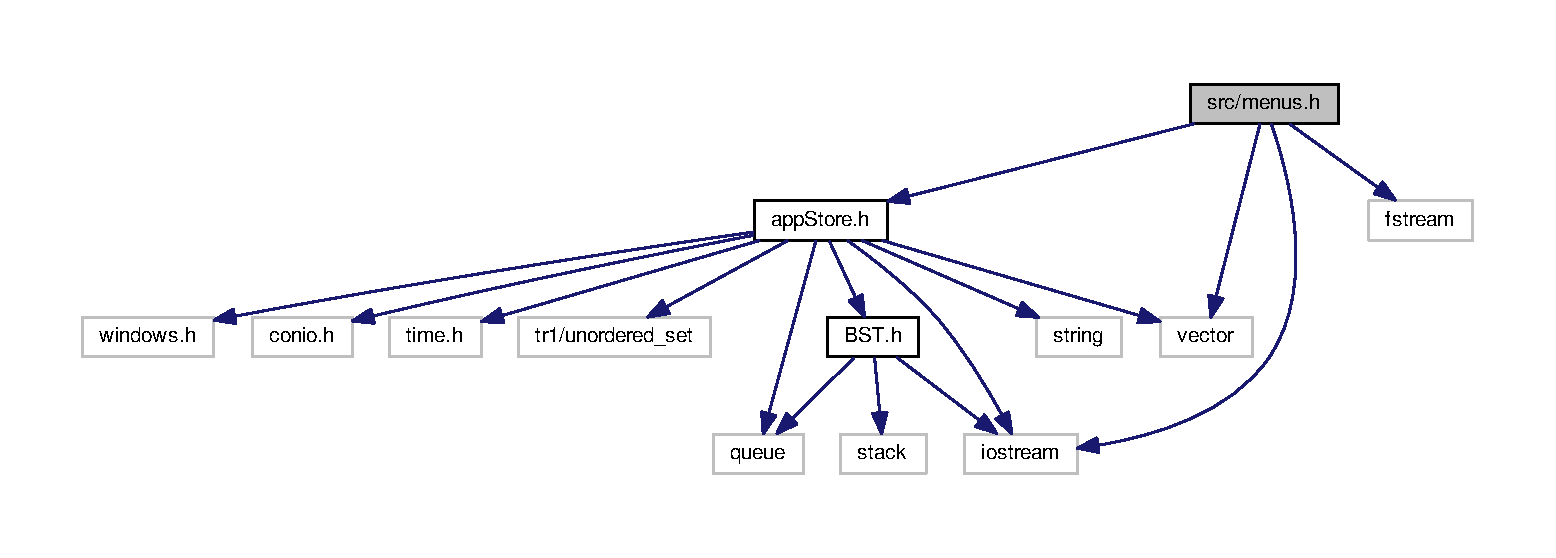
\includegraphics[width=350pt]{menus_8h__incl}
\end{center}
\end{figure}
This graph shows which files directly or indirectly include this file\-:
\nopagebreak
\begin{figure}[H]
\begin{center}
\leavevmode
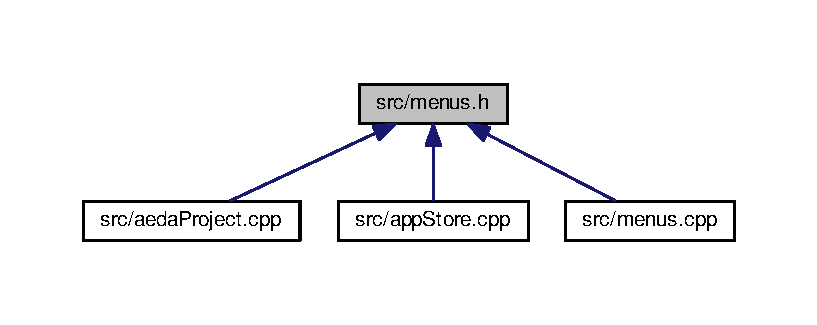
\includegraphics[width=350pt]{menus_8h__dep__incl}
\end{center}
\end{figure}
\subsection*{Functions}
\begin{DoxyCompactItemize}
\item 
void \hyperlink{menus_8h_aa585ae7d8f5362da92ce8e632e96c1ac}{cs} ()
\begin{DoxyCompactList}\small\item\em clears screen \end{DoxyCompactList}\item 
void \hyperlink{menus_8h_a7167f5c196fc5e167bfabde1a730e81d}{pause} ()
\begin{DoxyCompactList}\small\item\em pauses the program \end{DoxyCompactList}\item 
void \hyperlink{menus_8h_a1a6a7739e9cc01ba888b57d1f9457f4c}{Exit} ()
\begin{DoxyCompactList}\small\item\em Exit function. \end{DoxyCompactList}\item 
int \hyperlink{menus_8h_a00835efb53f4d81f809220267fe4991c}{first\-Screen} ()
\begin{DoxyCompactList}\small\item\em Shows the first screen. \end{DoxyCompactList}\item 
int \hyperlink{menus_8h_a4f88eaae08853208b5bb525d3e03da9d}{sign\-Up\-Menu} (\hyperlink{class_app_store}{App\-Store} \&apps)
\begin{DoxyCompactList}\small\item\em Controls the sign up menu. \end{DoxyCompactList}\item 
bool \hyperlink{menus_8h_a44b193a809749f66e7928ef86f50f7d9}{checkusername} (string u, \hyperlink{class_app_store}{App\-Store} \&app)
\begin{DoxyCompactList}\small\item\em Checks the username. \end{DoxyCompactList}\item 
int \hyperlink{menus_8h_acc8e8a27a849a306e1dbfa836c5a07b4}{Menu} (int a, \hyperlink{class_app_store}{App\-Store} \&appstore)
\begin{DoxyCompactList}\small\item\em function to redirect to menu type \end{DoxyCompactList}\item 
int \hyperlink{menus_8h_a23a082437ea9566917fc09f1d2ccc7b0}{login\-Menu} (\hyperlink{class_app_store}{App\-Store} \&apps)
\begin{DoxyCompactList}\small\item\em Controls the login menu. \end{DoxyCompactList}\item 
int \hyperlink{menus_8h_a17c7e9490a26e40c5d3c6382728b3e36}{check\-User} (string username, string password, \hyperlink{class_app_store}{App\-Store} \&apps)
\begin{DoxyCompactList}\small\item\em Checks user for the right password. \end{DoxyCompactList}\item 
vector$<$ \hyperlink{class_app}{App} $>$ \hyperlink{menus_8h_ab397273ffad40b9e8c08bd27138390e8}{read\-Apps} (\hyperlink{class_app_store}{App\-Store} \&apps)
\begin{DoxyCompactList}\small\item\em Function to read Apps info from text file. \end{DoxyCompactList}\item 
vector$<$ \hyperlink{class_client}{Client} $>$ \hyperlink{menus_8h_abb046e57ad494277538d50511a16553f}{read\-Clients} (\hyperlink{class_app_store}{App\-Store} \&apps)
\begin{DoxyCompactList}\small\item\em Function to read clients info from text file. \end{DoxyCompactList}\item 
vector$<$ \hyperlink{class_developer}{Developer} $>$ \hyperlink{menus_8h_af9a05ef922cdb113a8fe7898cf62b8b9}{read\-Devs} (\hyperlink{class_app_store}{App\-Store} \&apps)
\begin{DoxyCompactList}\small\item\em Function to read Devs info from text file. \end{DoxyCompactList}\item 
vector$<$ \hyperlink{class_company}{Company} $>$ \hyperlink{menus_8h_affb2cadd67c8096436d9a8f06279afe3}{read\-Comp} (\hyperlink{class_app_store}{App\-Store} \&apps)
\begin{DoxyCompactList}\small\item\em Function to read Companies info from text file. \end{DoxyCompactList}\item 
void \hyperlink{menus_8h_afcd035b559f35fd9ea1e862a3fd109ea}{read\-Appsto\-Bst} (\hyperlink{class_app_store}{App\-Store} \&apps)
\item 
void \hyperlink{menus_8h_ad0841b67a9be8040effd43726dd92267}{write\-Apps\-To\-Bst} (\hyperlink{class_b_s_t}{B\-S\-T}$<$ \hyperlink{class_app_to_bst}{App\-To\-Bst} $>$ app)
\begin{DoxyCompactList}\small\item\em Function to write Apps info to text file. \end{DoxyCompactList}\item 
void \hyperlink{menus_8h_a3b6ebfa15859dd53d6926f1886ad5789}{write\-Apps} (vector$<$ \hyperlink{class_app}{App} $>$ \&v)
\item 
void \hyperlink{menus_8h_a9a14a4f6d31bbdb53e01979851e5c2ba}{write\-Clients} (vector$<$ \hyperlink{class_client}{Client} $>$ c)
\begin{DoxyCompactList}\small\item\em Function to write clients info to text file. \end{DoxyCompactList}\item 
void \hyperlink{menus_8h_aa23062ec4ea8aab93c945f37580c2cbb}{write\-Devs} (\hyperlink{class_app_store}{App\-Store} \&apps)
\begin{DoxyCompactList}\small\item\em Function to write Devs info to text file. \end{DoxyCompactList}\item 
void \hyperlink{menus_8h_ac3a783d5fc67b458f098d4866be3160d}{write\-Comp} (vector$<$ \hyperlink{class_company}{Company} $>$ vd)
\begin{DoxyCompactList}\small\item\em Function to write Companies info to text file. \end{DoxyCompactList}\item 
int \hyperlink{menus_8h_a94b9006ef6c437e3ee9687ac2eeb2f0a}{buy\-Apps} (\hyperlink{class_app_store}{App\-Store} \&apps)
\item 
vector$<$ string $>$ \hyperlink{menus_8h_a1843c99b6b486725f2f24de1ace88ca0}{read\-Codes} (\hyperlink{class_app_store}{App\-Store} \&apps)
\begin{DoxyCompactList}\small\item\em Function to read Codes from text file. \end{DoxyCompactList}\item 
vector$<$ \hyperlink{class_sale}{Sale} $>$ \hyperlink{menus_8h_ae6ced19845f6d11c2269530c97134e6d}{read\-Sales} (\hyperlink{class_app_store}{App\-Store} \&apps)
\begin{DoxyCompactList}\small\item\em Function to read Codes from text file. \end{DoxyCompactList}\item 
void \hyperlink{menus_8h_a9d0b2bd4c24cec3b5f6c45068afe44b8}{write\-Sales} (vector$<$ \hyperlink{class_sale}{Sale} $>$ vd)
\begin{DoxyCompactList}\small\item\em Function to write sales to text file. \end{DoxyCompactList}\item 
float \hyperlink{menus_8h_ab564bbf34f9eacdf62fe5e4bd6fbca9b}{average} (\hyperlink{class_app}{App} $\ast$a, vector$<$ \hyperlink{class_client}{Client} $>$ clients)
\begin{DoxyCompactList}\small\item\em gets the average of an \hyperlink{class_app}{App}'s classification \end{DoxyCompactList}\item 
void \hyperlink{menus_8h_a550ef521ba111e4b2bcd7b151b28d991}{top10menu} (\hyperlink{class_app_store}{App\-Store} apps)
\begin{DoxyCompactList}\small\item\em Function to show apps from \hyperlink{class_b_s_t}{B\-S\-T}. \end{DoxyCompactList}\item 
void \hyperlink{menus_8h_a00da6ecf054736e0e2000d32ae1d1d2a}{write\-Vals} (\hyperlink{class_app_store}{App\-Store} \&apps)
\begin{DoxyCompactList}\small\item\em Write Apps waiting for validation info to text file. \end{DoxyCompactList}\item 
void \hyperlink{menus_8h_a0dfea7d90f0a83afe03b09acb925ff22}{read\-Vals} (\hyperlink{class_app_store}{App\-Store} \&apps)
\begin{DoxyCompactList}\small\item\em Function read validations from text file. \end{DoxyCompactList}\item 
void \hyperlink{menus_8h_a5a0785ff6e3adff536f33fb89b673290}{Admin\-B\-S\-T} (\hyperlink{class_app_store}{App\-Store} \&apps)
\begin{DoxyCompactList}\small\item\em C\-R\-U\-D Menu for \hyperlink{class_b_s_t}{B\-S\-T}. \end{DoxyCompactList}\end{DoxyCompactItemize}


\subsection{Function Documentation}
\hypertarget{menus_8h_a5a0785ff6e3adff536f33fb89b673290}{\index{menus.\-h@{menus.\-h}!Admin\-B\-S\-T@{Admin\-B\-S\-T}}
\index{Admin\-B\-S\-T@{Admin\-B\-S\-T}!menus.h@{menus.\-h}}
\subsubsection[{Admin\-B\-S\-T}]{\setlength{\rightskip}{0pt plus 5cm}void Admin\-B\-S\-T (
\begin{DoxyParamCaption}
\item[{{\bf App\-Store} \&}]{apps}
\end{DoxyParamCaption}
)}}\label{menus_8h_a5a0785ff6e3adff536f33fb89b673290}


C\-R\-U\-D Menu for \hyperlink{class_b_s_t}{B\-S\-T}. 


\begin{DoxyParams}{Parameters}
{\em apps} & \hyperlink{class_app_store}{App\-Store} \\
\hline
\end{DoxyParams}


Definition at line 1254 of file menus.\-cpp.

\hypertarget{menus_8h_ab564bbf34f9eacdf62fe5e4bd6fbca9b}{\index{menus.\-h@{menus.\-h}!average@{average}}
\index{average@{average}!menus.h@{menus.\-h}}
\subsubsection[{average}]{\setlength{\rightskip}{0pt plus 5cm}float average (
\begin{DoxyParamCaption}
\item[{{\bf App} $\ast$}]{a, }
\item[{vector$<$ {\bf Client} $>$}]{clients}
\end{DoxyParamCaption}
)}}\label{menus_8h_ab564bbf34f9eacdf62fe5e4bd6fbca9b}


gets the average of an \hyperlink{class_app}{App}'s classification 


\begin{DoxyParams}{Parameters}
{\em $\ast$a} & \hyperlink{class_app}{App} \\
\hline
{\em clients} & vector of the clients\\
\hline
\end{DoxyParams}
\begin{DoxyReturn}{Returns}
returns the average classification 
\end{DoxyReturn}


Definition at line 329 of file menus.\-cpp.

\hypertarget{menus_8h_a94b9006ef6c437e3ee9687ac2eeb2f0a}{\index{menus.\-h@{menus.\-h}!buy\-Apps@{buy\-Apps}}
\index{buy\-Apps@{buy\-Apps}!menus.h@{menus.\-h}}
\subsubsection[{buy\-Apps}]{\setlength{\rightskip}{0pt plus 5cm}int buy\-Apps (
\begin{DoxyParamCaption}
\item[{{\bf App\-Store} \&}]{apps}
\end{DoxyParamCaption}
)}}\label{menus_8h_a94b9006ef6c437e3ee9687ac2eeb2f0a}
shows and controls the menu of the clients purchase


\begin{DoxyParams}{Parameters}
{\em apps} & \hyperlink{class_app_store}{App\-Store}\\
\hline
\end{DoxyParams}
\begin{DoxyReturn}{Returns}
Returns 1 
\end{DoxyReturn}


Definition at line 451 of file menus.\-cpp.

\hypertarget{menus_8h_a17c7e9490a26e40c5d3c6382728b3e36}{\index{menus.\-h@{menus.\-h}!check\-User@{check\-User}}
\index{check\-User@{check\-User}!menus.h@{menus.\-h}}
\subsubsection[{check\-User}]{\setlength{\rightskip}{0pt plus 5cm}int check\-User (
\begin{DoxyParamCaption}
\item[{string}]{username, }
\item[{string}]{password, }
\item[{{\bf App\-Store} \&}]{apps}
\end{DoxyParamCaption}
)}}\label{menus_8h_a17c7e9490a26e40c5d3c6382728b3e36}


Checks user for the right password. 


\begin{DoxyParams}{Parameters}
{\em username} & name of the user \\
\hline
{\em password} & password of theuser \\
\hline
{\em apps} & Apps\\
\hline
\end{DoxyParams}
\begin{DoxyReturn}{Returns}
returns 0-\/2 
\end{DoxyReturn}


Definition at line 292 of file menus.\-cpp.

\hypertarget{menus_8h_a44b193a809749f66e7928ef86f50f7d9}{\index{menus.\-h@{menus.\-h}!checkusername@{checkusername}}
\index{checkusername@{checkusername}!menus.h@{menus.\-h}}
\subsubsection[{checkusername}]{\setlength{\rightskip}{0pt plus 5cm}bool checkusername (
\begin{DoxyParamCaption}
\item[{string}]{username, }
\item[{{\bf App\-Store} \&}]{apps}
\end{DoxyParamCaption}
)}}\label{menus_8h_a44b193a809749f66e7928ef86f50f7d9}


Checks the username. 


\begin{DoxyParams}{Parameters}
{\em username} & the username to check \\
\hline
{\em apps} & with the info\\
\hline
\end{DoxyParams}
\begin{DoxyReturn}{Returns}
returns true/false depending on que check of the username 
\end{DoxyReturn}


Definition at line 244 of file menus.\-cpp.

\hypertarget{menus_8h_aa585ae7d8f5362da92ce8e632e96c1ac}{\index{menus.\-h@{menus.\-h}!cs@{cs}}
\index{cs@{cs}!menus.h@{menus.\-h}}
\subsubsection[{cs}]{\setlength{\rightskip}{0pt plus 5cm}void cs (
\begin{DoxyParamCaption}
{}
\end{DoxyParamCaption}
)}}\label{menus_8h_aa585ae7d8f5362da92ce8e632e96c1ac}


clears screen 



Definition at line 62 of file menus.\-cpp.

\hypertarget{menus_8h_a1a6a7739e9cc01ba888b57d1f9457f4c}{\index{menus.\-h@{menus.\-h}!Exit@{Exit}}
\index{Exit@{Exit}!menus.h@{menus.\-h}}
\subsubsection[{Exit}]{\setlength{\rightskip}{0pt plus 5cm}void Exit (
\begin{DoxyParamCaption}
\item[{void}]{}
\end{DoxyParamCaption}
)}}\label{menus_8h_a1a6a7739e9cc01ba888b57d1f9457f4c}


Exit function. 

defgroup Menus Menus

Controls the menus and the interface 

Definition at line 11 of file menus.\-cpp.

\hypertarget{menus_8h_a00835efb53f4d81f809220267fe4991c}{\index{menus.\-h@{menus.\-h}!first\-Screen@{first\-Screen}}
\index{first\-Screen@{first\-Screen}!menus.h@{menus.\-h}}
\subsubsection[{first\-Screen}]{\setlength{\rightskip}{0pt plus 5cm}int first\-Screen (
\begin{DoxyParamCaption}
{}
\end{DoxyParamCaption}
)}}\label{menus_8h_a00835efb53f4d81f809220267fe4991c}


Shows the first screen. 



Definition at line 75 of file menus.\-cpp.

\hypertarget{menus_8h_a23a082437ea9566917fc09f1d2ccc7b0}{\index{menus.\-h@{menus.\-h}!login\-Menu@{login\-Menu}}
\index{login\-Menu@{login\-Menu}!menus.h@{menus.\-h}}
\subsubsection[{login\-Menu}]{\setlength{\rightskip}{0pt plus 5cm}int login\-Menu (
\begin{DoxyParamCaption}
\item[{{\bf App\-Store} \&}]{apps}
\end{DoxyParamCaption}
)}}\label{menus_8h_a23a082437ea9566917fc09f1d2ccc7b0}


Controls the login menu. 


\begin{DoxyParams}{Parameters}
{\em apps} & \hyperlink{class_app_store}{App\-Store}\\
\hline
\end{DoxyParams}
\begin{DoxyReturn}{Returns}
returns 0 
\end{DoxyReturn}


Definition at line 209 of file menus.\-cpp.

\hypertarget{menus_8h_acc8e8a27a849a306e1dbfa836c5a07b4}{\index{menus.\-h@{menus.\-h}!Menu@{Menu}}
\index{Menu@{Menu}!menus.h@{menus.\-h}}
\subsubsection[{Menu}]{\setlength{\rightskip}{0pt plus 5cm}int Menu (
\begin{DoxyParamCaption}
\item[{int}]{a, }
\item[{{\bf App\-Store} \&}]{apps}
\end{DoxyParamCaption}
)}}\label{menus_8h_acc8e8a27a849a306e1dbfa836c5a07b4}


function to redirect to menu type 


\begin{DoxyParams}{Parameters}
{\em apps} & \hyperlink{class_app_store}{App\-Store} \\
\hline
{\em a} & type of menun (from 1 to 3) \\
\hline
\end{DoxyParams}


Definition at line 1543 of file menus.\-cpp.

\hypertarget{menus_8h_a7167f5c196fc5e167bfabde1a730e81d}{\index{menus.\-h@{menus.\-h}!pause@{pause}}
\index{pause@{pause}!menus.h@{menus.\-h}}
\subsubsection[{pause}]{\setlength{\rightskip}{0pt plus 5cm}void pause (
\begin{DoxyParamCaption}
{}
\end{DoxyParamCaption}
)}}\label{menus_8h_a7167f5c196fc5e167bfabde1a730e81d}


pauses the program 



Definition at line 67 of file menus.\-cpp.

\hypertarget{menus_8h_ab397273ffad40b9e8c08bd27138390e8}{\index{menus.\-h@{menus.\-h}!read\-Apps@{read\-Apps}}
\index{read\-Apps@{read\-Apps}!menus.h@{menus.\-h}}
\subsubsection[{read\-Apps}]{\setlength{\rightskip}{0pt plus 5cm}vector$<${\bf App}$>$ read\-Apps (
\begin{DoxyParamCaption}
\item[{{\bf App\-Store} \&}]{apps}
\end{DoxyParamCaption}
)}}\label{menus_8h_ab397273ffad40b9e8c08bd27138390e8}


Function to read Apps info from text file. 


\begin{DoxyParams}{Parameters}
{\em apps} & \hyperlink{class_app_store}{App\-Store} \\
\hline
\end{DoxyParams}
\begin{DoxyReturn}{Returns}
vector of apps 
\end{DoxyReturn}


Definition at line 1685 of file menus.\-cpp.

\hypertarget{menus_8h_afcd035b559f35fd9ea1e862a3fd109ea}{\index{menus.\-h@{menus.\-h}!read\-Appsto\-Bst@{read\-Appsto\-Bst}}
\index{read\-Appsto\-Bst@{read\-Appsto\-Bst}!menus.h@{menus.\-h}}
\subsubsection[{read\-Appsto\-Bst}]{\setlength{\rightskip}{0pt plus 5cm}void read\-Appsto\-Bst (
\begin{DoxyParamCaption}
\item[{{\bf App\-Store} \&}]{apps}
\end{DoxyParamCaption}
)}}\label{menus_8h_afcd035b559f35fd9ea1e862a3fd109ea}


Definition at line 1720 of file menus.\-cpp.

\hypertarget{menus_8h_abb046e57ad494277538d50511a16553f}{\index{menus.\-h@{menus.\-h}!read\-Clients@{read\-Clients}}
\index{read\-Clients@{read\-Clients}!menus.h@{menus.\-h}}
\subsubsection[{read\-Clients}]{\setlength{\rightskip}{0pt plus 5cm}vector$<${\bf Client}$>$ read\-Clients (
\begin{DoxyParamCaption}
\item[{{\bf App\-Store} \&}]{apps}
\end{DoxyParamCaption}
)}}\label{menus_8h_abb046e57ad494277538d50511a16553f}


Function to read clients info from text file. 


\begin{DoxyParams}{Parameters}
{\em apps} & \hyperlink{class_app_store}{App\-Store} \\
\hline
\end{DoxyParams}


Definition at line 1590 of file menus.\-cpp.

\hypertarget{menus_8h_a1843c99b6b486725f2f24de1ace88ca0}{\index{menus.\-h@{menus.\-h}!read\-Codes@{read\-Codes}}
\index{read\-Codes@{read\-Codes}!menus.h@{menus.\-h}}
\subsubsection[{read\-Codes}]{\setlength{\rightskip}{0pt plus 5cm}vector$<$string$>$ read\-Codes (
\begin{DoxyParamCaption}
\item[{{\bf App\-Store} \&}]{apps}
\end{DoxyParamCaption}
)}}\label{menus_8h_a1843c99b6b486725f2f24de1ace88ca0}


Function to read Codes from text file. 


\begin{DoxyParams}{Parameters}
{\em apps} & \hyperlink{class_app_store}{App\-Store} \\
\hline
\end{DoxyParams}
\begin{DoxyReturn}{Returns}
vector of strings with codes 
\end{DoxyReturn}


Definition at line 1984 of file menus.\-cpp.

\hypertarget{menus_8h_affb2cadd67c8096436d9a8f06279afe3}{\index{menus.\-h@{menus.\-h}!read\-Comp@{read\-Comp}}
\index{read\-Comp@{read\-Comp}!menus.h@{menus.\-h}}
\subsubsection[{read\-Comp}]{\setlength{\rightskip}{0pt plus 5cm}vector$<${\bf Company}$>$ read\-Comp (
\begin{DoxyParamCaption}
\item[{{\bf App\-Store} \&}]{apps}
\end{DoxyParamCaption}
)}}\label{menus_8h_affb2cadd67c8096436d9a8f06279afe3}


Function to read Companies info from text file. 


\begin{DoxyParams}{Parameters}
{\em apps} & \hyperlink{class_app_store}{App\-Store} \\
\hline
\end{DoxyParams}
\begin{DoxyReturn}{Returns}
vector of companies 
\end{DoxyReturn}


Definition at line 1896 of file menus.\-cpp.

\hypertarget{menus_8h_af9a05ef922cdb113a8fe7898cf62b8b9}{\index{menus.\-h@{menus.\-h}!read\-Devs@{read\-Devs}}
\index{read\-Devs@{read\-Devs}!menus.h@{menus.\-h}}
\subsubsection[{read\-Devs}]{\setlength{\rightskip}{0pt plus 5cm}vector$<${\bf Developer}$>$ read\-Devs (
\begin{DoxyParamCaption}
\item[{{\bf App\-Store} \&}]{apps}
\end{DoxyParamCaption}
)}}\label{menus_8h_af9a05ef922cdb113a8fe7898cf62b8b9}


Function to read Devs info from text file. 


\begin{DoxyParams}{Parameters}
{\em apps} & \hyperlink{class_app_store}{App\-Store} \\
\hline
\end{DoxyParams}
\begin{DoxyReturn}{Returns}
vector of Devs 
\end{DoxyReturn}


Definition at line 1802 of file menus.\-cpp.

\hypertarget{menus_8h_ae6ced19845f6d11c2269530c97134e6d}{\index{menus.\-h@{menus.\-h}!read\-Sales@{read\-Sales}}
\index{read\-Sales@{read\-Sales}!menus.h@{menus.\-h}}
\subsubsection[{read\-Sales}]{\setlength{\rightskip}{0pt plus 5cm}vector$<${\bf Sale}$>$ read\-Sales (
\begin{DoxyParamCaption}
\item[{{\bf App\-Store} \&}]{apps}
\end{DoxyParamCaption}
)}}\label{menus_8h_ae6ced19845f6d11c2269530c97134e6d}


Function to read Codes from text file. 


\begin{DoxyParams}{Parameters}
{\em apps} & \hyperlink{class_app_store}{App\-Store} \\
\hline
\end{DoxyParams}
\begin{DoxyReturn}{Returns}
vector of strings with codes 
\end{DoxyReturn}


Definition at line 2009 of file menus.\-cpp.

\hypertarget{menus_8h_a0dfea7d90f0a83afe03b09acb925ff22}{\index{menus.\-h@{menus.\-h}!read\-Vals@{read\-Vals}}
\index{read\-Vals@{read\-Vals}!menus.h@{menus.\-h}}
\subsubsection[{read\-Vals}]{\setlength{\rightskip}{0pt plus 5cm}void read\-Vals (
\begin{DoxyParamCaption}
\item[{{\bf App\-Store} \&}]{apps}
\end{DoxyParamCaption}
)}}\label{menus_8h_a0dfea7d90f0a83afe03b09acb925ff22}


Function read validations from text file. 


\begin{DoxyParams}{Parameters}
{\em apps} & \hyperlink{class_app_store}{App\-Store} Data Structure \\
\hline
\end{DoxyParams}


Definition at line 2157 of file menus.\-cpp.

\hypertarget{menus_8h_a4f88eaae08853208b5bb525d3e03da9d}{\index{menus.\-h@{menus.\-h}!sign\-Up\-Menu@{sign\-Up\-Menu}}
\index{sign\-Up\-Menu@{sign\-Up\-Menu}!menus.h@{menus.\-h}}
\subsubsection[{sign\-Up\-Menu}]{\setlength{\rightskip}{0pt plus 5cm}int sign\-Up\-Menu (
\begin{DoxyParamCaption}
\item[{{\bf App\-Store} \&}]{apps}
\end{DoxyParamCaption}
)}}\label{menus_8h_a4f88eaae08853208b5bb525d3e03da9d}


Controls the sign up menu. 


\begin{DoxyParams}{Parameters}
{\em apps} & \hyperlink{class_app_store}{App\-Store}\\
\hline
\end{DoxyParams}
\begin{DoxyReturn}{Returns}
Returns 1 
\end{DoxyReturn}


Definition at line 125 of file menus.\-cpp.

\hypertarget{menus_8h_a550ef521ba111e4b2bcd7b151b28d991}{\index{menus.\-h@{menus.\-h}!top10menu@{top10menu}}
\index{top10menu@{top10menu}!menus.h@{menus.\-h}}
\subsubsection[{top10menu}]{\setlength{\rightskip}{0pt plus 5cm}void top10menu (
\begin{DoxyParamCaption}
\item[{{\bf App\-Store}}]{apps}
\end{DoxyParamCaption}
)}}\label{menus_8h_a550ef521ba111e4b2bcd7b151b28d991}


Function to show apps from \hyperlink{class_b_s_t}{B\-S\-T}. 


\begin{DoxyParams}{Parameters}
{\em apps} & \hyperlink{class_app_store}{App\-Store} \\
\hline
\end{DoxyParams}


Definition at line 2085 of file menus.\-cpp.

\hypertarget{menus_8h_a3b6ebfa15859dd53d6926f1886ad5789}{\index{menus.\-h@{menus.\-h}!write\-Apps@{write\-Apps}}
\index{write\-Apps@{write\-Apps}!menus.h@{menus.\-h}}
\subsubsection[{write\-Apps}]{\setlength{\rightskip}{0pt plus 5cm}void write\-Apps (
\begin{DoxyParamCaption}
\item[{vector$<$ {\bf App} $>$ \&}]{v}
\end{DoxyParamCaption}
)}}\label{menus_8h_a3b6ebfa15859dd53d6926f1886ad5789}


Definition at line 1770 of file menus.\-cpp.

\hypertarget{menus_8h_ad0841b67a9be8040effd43726dd92267}{\index{menus.\-h@{menus.\-h}!write\-Apps\-To\-Bst@{write\-Apps\-To\-Bst}}
\index{write\-Apps\-To\-Bst@{write\-Apps\-To\-Bst}!menus.h@{menus.\-h}}
\subsubsection[{write\-Apps\-To\-Bst}]{\setlength{\rightskip}{0pt plus 5cm}void write\-Apps\-To\-Bst (
\begin{DoxyParamCaption}
\item[{{\bf B\-S\-T}$<$ {\bf App\-To\-Bst} $>$}]{app}
\end{DoxyParamCaption}
)}}\label{menus_8h_ad0841b67a9be8040effd43726dd92267}


Function to write Apps info to text file. 


\begin{DoxyParams}{Parameters}
{\em apps} & \hyperlink{class_app_store}{App\-Store} \\
\hline
\end{DoxyParams}


Definition at line 1749 of file menus.\-cpp.

\hypertarget{menus_8h_a9a14a4f6d31bbdb53e01979851e5c2ba}{\index{menus.\-h@{menus.\-h}!write\-Clients@{write\-Clients}}
\index{write\-Clients@{write\-Clients}!menus.h@{menus.\-h}}
\subsubsection[{write\-Clients}]{\setlength{\rightskip}{0pt plus 5cm}void write\-Clients (
\begin{DoxyParamCaption}
\item[{vector$<$ {\bf Client} $>$}]{vc}
\end{DoxyParamCaption}
)}}\label{menus_8h_a9a14a4f6d31bbdb53e01979851e5c2ba}


Function to write clients info to text file. 


\begin{DoxyParams}{Parameters}
{\em apps} & \hyperlink{class_app_store}{App\-Store} \\
\hline
\end{DoxyParams}


Definition at line 1648 of file menus.\-cpp.

\hypertarget{menus_8h_ac3a783d5fc67b458f098d4866be3160d}{\index{menus.\-h@{menus.\-h}!write\-Comp@{write\-Comp}}
\index{write\-Comp@{write\-Comp}!menus.h@{menus.\-h}}
\subsubsection[{write\-Comp}]{\setlength{\rightskip}{0pt plus 5cm}void write\-Comp (
\begin{DoxyParamCaption}
\item[{vector$<$ {\bf Company} $>$}]{vd}
\end{DoxyParamCaption}
)}}\label{menus_8h_ac3a783d5fc67b458f098d4866be3160d}


Function to write Companies info to text file. 


\begin{DoxyParams}{Parameters}
{\em apps} & \hyperlink{class_app_store}{App\-Store} \\
\hline
\end{DoxyParams}


Definition at line 1948 of file menus.\-cpp.

\hypertarget{menus_8h_aa23062ec4ea8aab93c945f37580c2cbb}{\index{menus.\-h@{menus.\-h}!write\-Devs@{write\-Devs}}
\index{write\-Devs@{write\-Devs}!menus.h@{menus.\-h}}
\subsubsection[{write\-Devs}]{\setlength{\rightskip}{0pt plus 5cm}void write\-Devs (
\begin{DoxyParamCaption}
\item[{{\bf App\-Store} \&}]{apps}
\end{DoxyParamCaption}
)}}\label{menus_8h_aa23062ec4ea8aab93c945f37580c2cbb}


Function to write Devs info to text file. 


\begin{DoxyParams}{Parameters}
{\em apps} & \hyperlink{class_app_store}{App\-Store} \\
\hline
\end{DoxyParams}


Definition at line 1861 of file menus.\-cpp.

\hypertarget{menus_8h_a9d0b2bd4c24cec3b5f6c45068afe44b8}{\index{menus.\-h@{menus.\-h}!write\-Sales@{write\-Sales}}
\index{write\-Sales@{write\-Sales}!menus.h@{menus.\-h}}
\subsubsection[{write\-Sales}]{\setlength{\rightskip}{0pt plus 5cm}void write\-Sales (
\begin{DoxyParamCaption}
\item[{vector$<$ {\bf Sale} $>$}]{vd}
\end{DoxyParamCaption}
)}}\label{menus_8h_a9d0b2bd4c24cec3b5f6c45068afe44b8}


Function to write sales to text file. 


\begin{DoxyParams}{Parameters}
{\em vd} & Vector of sales \\
\hline
\end{DoxyParams}


Definition at line 2056 of file menus.\-cpp.

\hypertarget{menus_8h_a00da6ecf054736e0e2000d32ae1d1d2a}{\index{menus.\-h@{menus.\-h}!write\-Vals@{write\-Vals}}
\index{write\-Vals@{write\-Vals}!menus.h@{menus.\-h}}
\subsubsection[{write\-Vals}]{\setlength{\rightskip}{0pt plus 5cm}void write\-Vals (
\begin{DoxyParamCaption}
\item[{{\bf App\-Store} \&}]{apps}
\end{DoxyParamCaption}
)}}\label{menus_8h_a00da6ecf054736e0e2000d32ae1d1d2a}


Write Apps waiting for validation info to text file. 


\begin{DoxyParams}{Parameters}
{\em apps} & \hyperlink{class_app_store}{App\-Store} Data structure \\
\hline
\end{DoxyParams}


Definition at line 2207 of file menus.\-cpp.


%--- End generated contents ---

% Index
\newpage
\phantomsection
\addcontentsline{toc}{chapter}{Index}
\printindex

\end{document}
